\documentclass[a4paper,12pt]{article}

\usepackage[T1]{fontenc}
\usepackage[utf8]{inputenc}
\usepackage{indentfirst}
\usepackage{tgtermes}
\usepackage{geometry}
\geometry{a4paper,top=3cm,left=3cm,right=2cm,bottom=2cm}
\usepackage{setspace}
\usepackage{ragged2e}
\usepackage{microtype}
\usepackage{graphicx}
\usepackage{booktabs}
\usepackage{array}
\usepackage{tabularx}
\usepackage{amsmath}
\usepackage{float}
\usepackage{caption}
\usepackage{subcaption}
\usepackage{titlesec}
\usepackage{tocloft}
\usepackage{xurl}
\usepackage[hidelinks,hypertexnames=false]{hyperref}

\graphicspath{{../Imagens/}{../Imagens/Diagramas/teoricas/}{Imagens/}{Imagens/Diagramas/teoricas/}}

\onehalfspacing
\justifying
\setlength{\parindent}{1.27cm}
\setlength{\parskip}{0pt}
\setlength{\emergencystretch}{3em}
\setcounter{secnumdepth}{4}
\setcounter{tocdepth}{3}
\widowpenalty=10000
\clubpenalty=10000

\titleformat{\section}
  {\normalfont\bfseries\fontsize{12}{14}\selectfont}
  {\thesection}{1em}{\MakeUppercase}
\titleformat{\subsection}
  {\normalfont\fontsize{12}{14}\selectfont}
  {\thesubsection}{1em}{\MakeUppercase}
\titleformat{\subsubsection}
  {\normalfont\bfseries\fontsize{12}{14}\selectfont}
  {\thesubsubsection}{1em}{}
\titleformat{\paragraph}[hang]
  {\normalfont\itshape\fontsize{12}{14}\selectfont}
  {\theparagraph}{1em}{}
\titlespacing*{\section}{0pt}{1.5\baselineskip}{1\baselineskip}
\titlespacing*{\subsection}{0pt}{1.5\baselineskip}{1\baselineskip}
\titlespacing*{\subsubsection}{0pt}{1.25\baselineskip}{0.75\baselineskip}

\renewcommand{\figurename}{Figura}
\renewcommand{\tablename}{Tabela}
\renewcommand{\contentsname}{Sumário}
\renewcommand{\listfigurename}{Lista de figuras}
\renewcommand{\listtablename}{Lista de tabelas}
\DeclareCaptionLabelSeparator{travessao}{ -- }
\captionsetup{
  justification=raggedright,
  singlelinecheck=false,
  labelsep=travessao,
  font=normalsize,
  labelfont=bf,
  skip=6pt
}
\captionsetup[figure]{position=above}
\captionsetup[table]{position=above}
\newfloat{quadro}{htbp}{loq}
\floatname{quadro}{Quadro}
\captionsetup[quadro]{position=above}
\newcommand{\listadequadros}{\listof{quadro}{Lista de quadros}}
\newcommand{\fonteelemento}[1]{%
  \par\smallskip
  {\fontsize{10}{12}\selectfont\raggedright Fonte: #1.\par}%
}

\renewcommand{\cftsecfont}{\normalfont}
\renewcommand{\cftsecpagefont}{\normalfont}
\setlength{\cftbeforesecskip}{0pt}

\begin{document}
\pagenumbering{gobble}

\begin{titlepage}
\thispagestyle{empty}
\begin{center}

\includegraphics[width=0.20\textwidth]{General/ifsc-logo.png}

\vspace{0.8cm}

{\bfseries INSTITUTO FEDERAL DE SANTA CATARINA\par}
{\bfseries CÂMPUS FLORIANÓPOLIS\par}
{\bfseries CURSO DE ENGENHARIA ELETRÔNICA\par}

\vfill

{\bfseries GUILHERME DA COSTA FRANCO\par}

\vfill

{\bfseries DESENVOLVIMENTO DE UMA PLATAFORMA VESTÍVEL MODULAR
MULTISSENSOR BASEADA NO ESP32-C6\par}

\vfill

{\bfseries FLORIANÓPOLIS\par}
{\bfseries 2026\par}
\end{center}
\end{titlepage}

\begin{titlepage}
\thispagestyle{empty}
\begin{center}
{\bfseries GUILHERME DA COSTA FRANCO\par}

\vfill

{\bfseries DESENVOLVIMENTO DE UMA PLATAFORMA VESTÍVEL MODULAR
MULTISSENSOR BASEADA NO ESP32-C6\par}
\end{center}

\vspace{3cm}

\begin{flushright}
\begin{minipage}{0.52\textwidth}
\setlength{\parindent}{0pt}
\justifying
Trabalho de Conclusão de Curso apresentado ao Curso de Engenharia
Eletrônica do Instituto Federal de Santa Catarina, Câmpus
Florianópolis, como requisito parcial para obtenção do título de
Bacharel em Engenharia Eletrônica.

\vspace{0.8cm}

Orientador: Prof. Me. Leandro Schwarz.
\end{minipage}
\end{flushright}

\vfill

\begin{center}
{\bfseries FLORIANÓPOLIS\par}
{\bfseries 2026\par}
\end{center}
\end{titlepage}

\clearpage
\thispagestyle{empty}
\vspace*{\fill}
\begin{center}
\fbox{\begin{minipage}[c][6cm][c]{0.78\textwidth}
\centering
\textbf{FICHA CATALOGRÁFICA}

\vspace{0.7cm}

Campo reservado para a ficha catalográfica a ser fornecida pela
biblioteca do Instituto Federal de Santa Catarina.
\end{minipage}}
\end{center}
\vspace*{\fill}
\clearpage

\begin{titlepage}
\thispagestyle{empty}
\begin{center}
{\bfseries GUILHERME DA COSTA FRANCO\par}

\vspace{2cm}

{\bfseries DESENVOLVIMENTO DE UMA PLATAFORMA VESTÍVEL MODULAR
MULTISSENSOR BASEADA NO ESP32-C6\par}
\end{center}

\vspace{2cm}

\justifying
Este Trabalho de Conclusão de Curso foi julgado adequado para a
obtenção do título de Bacharel em Engenharia Eletrônica e aprovado em
sua forma final pelo Curso de Engenharia Eletrônica do Instituto
Federal de Santa Catarina, Câmpus Florianópolis.

\vspace{1.2cm}

\begin{center}
Florianópolis, \rule{1cm}{0.4pt} de \rule{3cm}{0.4pt} de 2026.

\vspace{1.5cm}

\rule{8cm}{0.4pt}\par
\vspace{0.2cm}
Prof. Me. Leandro Schwarz\par
Orientador\par

\vspace{1.5cm}

\textbf{BANCA EXAMINADORA}

\vspace{1.2cm}

\rule{8cm}{0.4pt}\par
\vspace{0.2cm}
Prof. Dr. Fernando Pedro Henriques de Miranda\par

\vspace{1.2cm}

\rule{8cm}{0.4pt}\par
\vspace{0.2cm}
Prof. Dr. Renan Augusto Starke\par
\end{center}
\end{titlepage}

\pagenumbering{roman}
\setcounter{page}{1}

\clearpage
\thispagestyle{empty}
\vspace*{\fill}
\begin{flushright}
\begin{minipage}{0.60\textwidth}
\setlength{\parindent}{0pt}
\justifying
Dedico este trabalho aos meus pais, pelo incentivo e apoio ao longo de
toda a minha formação acadêmica. Seguimos fazendo o melhor que podemos,
sem olhar para trás com pesar, sabendo que sempre há tempo de escolher
novos caminhos.
\end{minipage}
\end{flushright}
\vspace*{\fill}

\clearpage
\section*{Agradecimentos}
\addcontentsline{toc}{section}{Agradecimentos}

Agradeço, com todo o pudor da ironia, às minhas incontáveis tentativas
fracassadas de desistir da graduação, que tantas vezes circundaram minha
mente em momentos de fragilidade. Vivenciei na pele que o fracasso, por
mais dolorosa que essa experiência tenha sido, também pode servir de
alicerce para grandes fundações, principalmente quando deixamos de nos
guiar por uma ótica pessimista e pela tendência incontrolável de
subestimar a própria capacidade, sem que isso nos leve a diminuir o
outro ou a confundir confiança com soberba.

À minha família, seja ela definida por laços diretos ou por conexões que,
em um grafo afetivo, teriam peso infinitamente maior do que qualquer grau
de parentesco poderia sugerir. Em especial, agradeço à minha tia Zaira
Sinara, pelo acolhimento, pela orientação e pelo apoio nos momentos em
que precisei de firmeza e cuidado.

Agradeço também à minha prima Denise, que carinhosamente sempre chamei
de tia, por ter exercido esse mesmo papel com tanto amor, companheirismo
e risadas soltas. Vocês foram vértices fundamentais nessa trajetória,
conectando afeto, escuta e incentivo quando eu mais precisei, sem que
fosse necessário nenhum algoritmo de Dijkstra rodando ao fundo para me
mostrar o caminho mais curto.

Sou grato também aos meus amigos e colegas de profissão Marcelo
Zampieri, Caio Meira e Rafael Aquino, que foram protagonistas essenciais
em todos os altos e baixos da graduação, com sua camaradagem, parceria e
irreverência nos momentos mais desesperadores, como apresentações de
trabalhos feitos de última hora e torres de chope de vinho que chegavam
ao fim rápido demais.

Agradeço também aos meus amigos Juliana Andrade e Kevin Trovão, por
terem sido verdadeiros guardiões deste trabalho. O destino nos uniu em
um completo acaso e fez com que vocês também se tornassem parte
importante da minha jornada acadêmica. Entre conversas, apoio e
companheirismo, vocês me lembraram que nenhuma missão difícil precisa
ser enfrentada completamente sozinho quando se tem um bom esquadrão ao
lado.

Ao meu orientador, professor Leandro Schwarz, pelos conhecimentos
transmitidos, pela confiança depositada em minhas habilidades e por ter
enxergado em mim a capacidade de desenvolver um projeto do qual eu
pudesse me orgulhar. Agradeço imensamente pela orientação, pelo incentivo
e por ter contribuído para que este trabalho se tornasse não apenas a
conclusão de uma etapa acadêmica, mas também uma importante realização
pessoal.

E, por fim, agradeço ao Instituto Federal de Santa Catarina, instituição
que foi parte fundamental da minha formação acadêmica, profissional e
pessoal. Agradeço também aos professores do Departamento Acadêmico de
Eletrônica, pela excelência didática, pela dedicação ao ensino e pela
forma como conduziram, ao longo do curso, uma formação fortemente
baseada na experimentação, na prática e na construção concreta do
conhecimento.

Essa abordagem foi essencial para transformar conceitos teóricos em
aprendizado real, aproximando a engenharia dos desafios concretos da
prática profissional e despertando em mim maior interesse pela criação,
pela investigação e pela solução de problemas. Levo comigo, além dos
conteúdos aprendidos, a influência de uma formação que valoriza o
pensamento crítico, a autonomia e a capacidade de aprender fazendo.

\clearpage
\thispagestyle{empty}
\vspace*{\fill}
\begin{flushright}
\begin{minipage}{0.50\textwidth}
\setlength{\parindent}{0pt}
\raggedleft
``Kept you waiting, huh?''

\vspace{0.5cm}

--- Snake, \emph{Metal Gear}
\end{minipage}
\end{flushright}
\vspace*{\fill}

\clearpage
\section*{Resumo}
\addcontentsline{toc}{section}{Resumo}

Este trabalho apresenta o desenvolvimento e a avaliação de uma
plataforma vestível modular multissensor baseada no ESP32-C6. A versão
final integrou interface gráfica circular sensível ao toque, relógio de
tempo real, fotopletismografia, temperatura, iluminância, radiação
ultravioleta, bússola e pedômetro em uma mesma aplicação embarcada. O
método combinou testes isolados dos componentes, separação entre
driver, processamento e apresentação, integração incremental e regressão
das funções existentes. A arquitetura resultante emprega contratos de
ciclo de vida, tarefas independentes e serviços compartilhados para
concorrência, persistência e recuperação do barramento I²C. Os ensaios
confirmaram a navegação entre as telas, a aquisição e o tratamento dos
canais sensoriais, a continuidade da inicialização nos ensaios com
sensores ausentes e o funcionamento da leitura de bateria. Os resultados
demonstram o atendimento dos objetivos de integração e
modularidade e confirmam a plataforma como base técnica funcional para
novas extensões. O alcance da avaliação é funcional e arquitetural, sem
pretensão de certificação clínica ou metrológica.

\noindent\textbf{Palavras-chave}: sistemas embarcados; dispositivo
vestível; arquitetura modular; ESP32-C6; sensores; smartwatch;
integração multissensor; Internet das Coisas.

\clearpage
\section*{Abstract}
\addcontentsline{toc}{section}{Abstract}

This work presents the development and evaluation of a modular
multisensor wearable platform based on the ESP32-C6. The final version
integrated a circular touchscreen interface, a real-time clock,
photoplethysmography, temperature, illuminance, ultraviolet radiation,
compass and pedometer functions into a single embedded application. The
method combined standalone component tests, separation among driver,
processing and presentation, incremental integration and regression of
existing functions. The resulting architecture employs lifecycle
contracts, independent tasks and shared services for concurrency,
persistence and I²C bus recovery. The tests confirmed navigation among
screens, acquisition and processing of sensor channels, continued
initialization in tests with missing sensors, and operation of the
battery measurement. The results demonstrate that the integration
and modularity objectives were achieved and confirm the platform as a
functional technical foundation for further extensions. The evaluation
scope is functional and architectural and does not claim clinical or
metrological certification.

\noindent\textbf{Keywords}: embedded systems; wearable device; modular
architecture; ESP32-C6; sensors; smartwatch; multisensor integration;
Internet of Things.

\clearpage
\listoffigures
\addcontentsline{toc}{section}{Lista de figuras}

\clearpage
\listoftables
\addcontentsline{toc}{section}{Lista de tabelas}

\clearpage
\listadequadros
\addcontentsline{toc}{section}{Lista de quadros}

\clearpage
\tableofcontents

\clearpage
\pagenumbering{arabic}
\setcounter{page}{1}

\section{Introdu\c{c}\~ao}

\subsection{Contextualiza\c{c}\~ao}

Os dispositivos vest\'iveis combinam aquisi\c{c}\~ao de dados, processamento embarcado e intera\c{c}\~ao com o usu\'ario em plataformas sujeitas a restri\c{c}\~oes de dimens\~oes, mem\'oria, capacidade computacional e consumo de energia. A disponibilidade de microcontroladores com m\'ultiplos perif\'ericos, sensores miniaturizados e interfaces gr\'aficas tornou vi\'avel a constru\c{c}\~ao de sistemas capazes de reunir fun\c{c}\~oes biom\'etricas, ambientais e inerciais em um \'unico dispositivo. Essa integra\c{c}\~ao, entretanto, n\~ao depende apenas da conex\~ao el\'etrica dos componentes: exige uma organiza\c{c}\~ao de software que coordene diferentes protocolos de comunica\c{c}\~ao, taxas de aquisi\c{c}\~ao, requisitos de processamento e mecanismos de apresenta\c{c}\~ao dos dados (SENEVIRATNE et al., 2017; HESTER et al., 2016).

\`A medida que novos sensores s\~ao incorporados, uma aplica\c{c}\~ao organizada de forma monol\'itica tende a concentrar depend\^encias no n\'ucleo do firmware. Nesse cen\'ario, altera\c{c}\~oes em um subsistema podem repercutir nos demais, dispositivos que compartilham um barramento podem interferir entre si e a falha de um componente pode impedir a inicializa\c{c}\~ao de toda a aplica\c{c}\~ao. Em um sistema embarcado com sistema operacional de tempo real, a integra\c{c}\~ao tamb\'em envolve concorr\^encia entre tarefas, sincroniza\c{c}\~ao de recursos e defini\c{c}\~ao de prioridades, aspectos que precisam ser considerados para preservar a responsividade da interface e o acesso ordenado ao hardware (FREERTOS, 2026c; SHA; RAJKUMAR; LEHOCZKY, 1990).

Esses desafios s\~ao particularmente relevantes em uma plataforma vest\'ivel modular multissensor. Al\'em de acomodar dispositivos com transportes distintos, a plataforma deve permitir a evolu\c{c}\~ao do firmware sem exigir a reestrutura\c{c}\~ao do conjunto a cada nova funcionalidade. Tamb\'em \'e desej\'avel que fun\c{c}\~oes independentes permane\c{c}am dispon\'iveis quando um sensor estiver ausente ou apresentar falha.

\subsection{Defini\c{c}\~ao do problema}

O problema abordado consiste em organizar e integrar sensores heterog\^eneos, interface gr\'afica e servi\c{c}os compartilhados em um dispositivo vest\'ivel com recursos limitados, de modo que a inclus\~ao ou a falha de um m\'odulo n\~ao exija altera\c{c}\~oes disseminadas pelo firmware nem comprometa o funcionamento das fun\c{c}\~oes independentes. A plataforma deve, adicionalmente, coordenar o acesso concorrente ao barramento I$^2$C compartilhado e recuperar sua opera\c{c}\~ao ap\'os falhas de comunica\c{c}\~ao.

Diante desse contexto, formula-se a seguinte quest\~ao de projeto:

\begin{quote}
Como projetar uma plataforma de software modular para um dispositivo vest\'ivel baseado no ESP32-C6, capaz de integrar sensores heterog\^eneos, compartilhar recursos de comunica\c{c}\~ao e permanecer operacional diante da aus\^encia ou falha de m\'odulos?
\end{quote}

A aplica\c{c}\~ao demonstradora re\'une m\'odulos biom\'etricos, ambientais e inerciais, rel\'ogio em tempo real e interface gr\'afica sens\'ivel ao toque. A Figura~\ref{fig:plataforma-aplicacao} diferencia essa instancia\c{c}\~ao da base arquitetural reutiliz\'avel.


\begin{figure}[H]
\centering
\caption{Rela\c{c}\~ao entre a plataforma modular e a aplica\c{c}\~ao demonstradora}
\label{fig:plataforma-aplicacao}
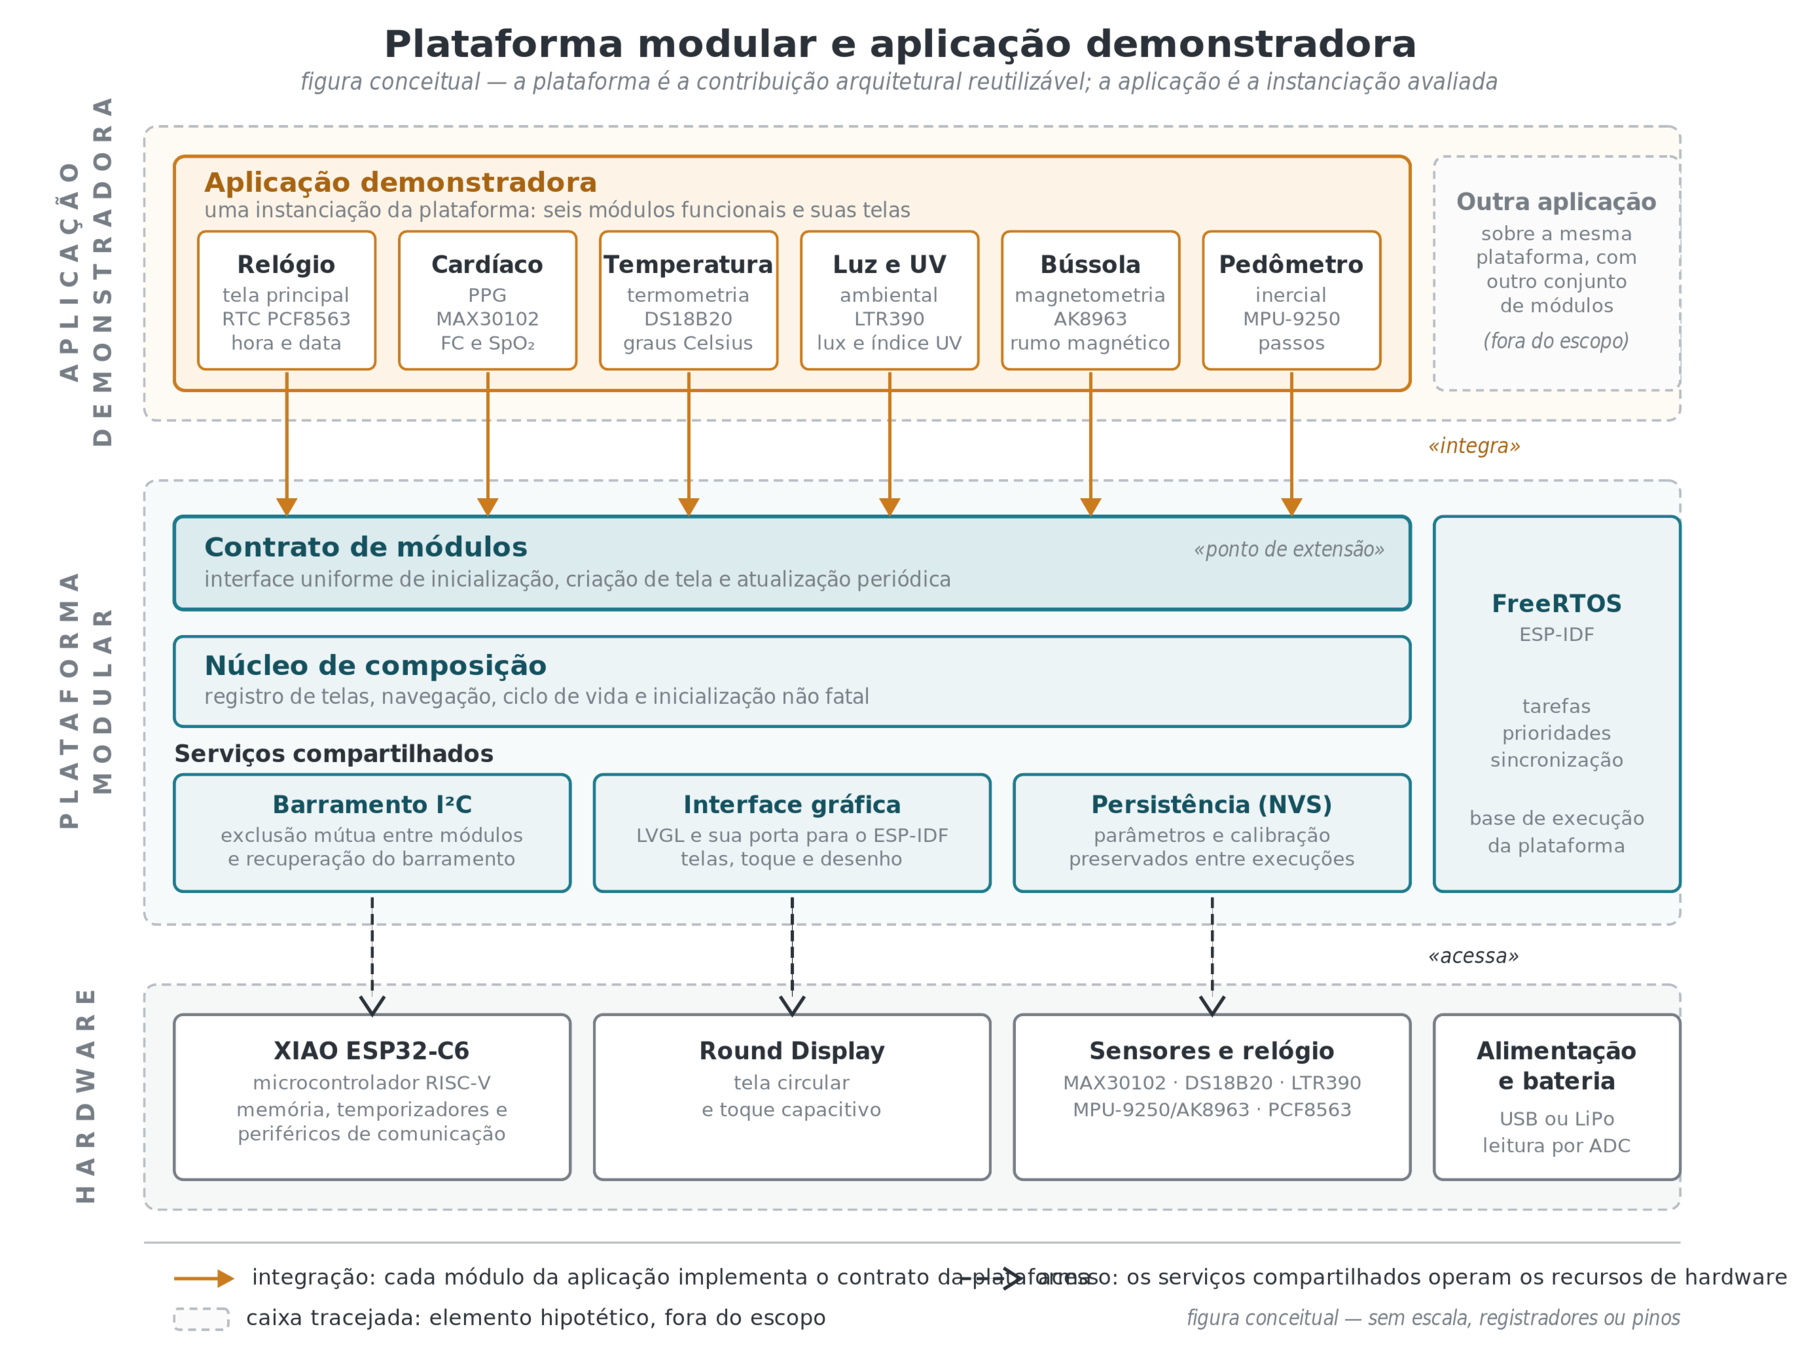
\includegraphics[width=0.96\textwidth]{Diagramas/teoricas/plataforma_aplicacao.png}
\fonteelemento{Elaborado pelo autor}
\end{figure}

\subsection{Objetivo geral}

Projetar e implementar uma plataforma vest\'ivel modular multissensor baseada no XIAO ESP32-C6, capaz de integrar sensores heterog\^eneos, interface gr\'afica e servi\c{c}os compartilhados, verificando estruturalmente sua extensibilidade e observando seu comportamento diante da aus\^encia de m\'odulos.

\subsection{Objetivos espec\'ificos}

Para alcan\c{c}ar o objetivo geral, s\~ao estabelecidos os seguintes objetivos espec\'ificos:

\begin{itemize}
    \item definir uma arquitetura modular para sensores e telas;
    \item estabelecer um contrato uniforme para inicializa\c{c}\~ao dos m\'odulos, cria\c{c}\~ao das telas e acesso \`as funcionalidades;
    \item implementar servi\c{c}os compartilhados de comunica\c{c}\~ao, interface gr\'afica e concorr\^encia;
    \item integrar m\'odulos biom\'etricos, ambientais e inerciais \`a aplica\c{c}\~ao demonstradora;
    \item implementar inicializa\c{c}\~ao n\~ao fatal, de modo que a plataforma possa operar com um subconjunto dos sensores;
    \item coordenar o acesso ao barramento I$^2$C compartilhado e implementar sua recupera\c{c}\~ao ap\'os falhas de comunica\c{c}\~ao;
    \item demonstrar a inclus\~ao de m\'odulos com impacto restrito sobre o n\'ucleo e sobre os m\'odulos existentes;
    \item avaliar o acoplamento, a extensibilidade, o uso est\'atico de mem\'oria e, dentro do escopo experimental, a estabilidade e os mecanismos de robustez da plataforma;
    \item realizar testes funcionais dos m\'odulos integrados; e
    \item produzir documenta\c{c}\~ao t\'ecnica que permita compreender e reproduzir as decis\~oes de arquitetura e integra\c{c}\~ao.
\end{itemize}

\subsection{Justificativa}

A relev\^ancia t\'ecnica do trabalho decorre do tratamento conjunto de problemas que surgem na integra\c{c}\~ao de um sistema embarcado multissensor. A coexist\^encia de dispositivos no mesmo barramento, a execu\c{c}\~ao concorrente de tarefas de aquisi\c{c}\~ao e interface, as diferen\c{c}as entre protocolos e a necessidade de preservar fun\c{c}\~oes independentes diante de falhas exigem decis\~oes que ultrapassam a implementa\c{c}\~ao isolada de drivers. Uma arquitetura com contrato uniforme, servi\c{c}os compartilhados e separa\c{c}\~ao entre n\'ucleo, servi\c{c}os, drivers e m\'odulos oferece uma base para controlar essas depend\^encias e tornar expl\'icitas as responsabilidades de cada parte (PARNAS, 1972; BASS; CLEMENTS; KAZMAN, 2021).

No \^ambito acad\^emico, o trabalho permite discutir a aplica\c{c}\~ao de conceitos de modularidade, extensibilidade, concorr\^encia e toler\^ancia a falhas em uma plataforma embarcada concreta. A escolha do ESP-IDF e do FreeRTOS fornece acesso aos mecanismos de tarefas, prioridades, sincroniza\c{c}\~ao, perif\'ericos e diagn\'ostico empregados na implementa\c{c}\~ao.

Do ponto de vista pr\'atico, a plataforma re\'une m\'odulos com caracter\'isticas distintas: o MAX30102 para fotopletismografia e estimativas de frequ\^encia card\'iaca e SpO$_2$; o DS18B20 para temperatura; o LTR390 para ilumin\^ancia e \'indice UV; e o conjunto MPU-9250/AK8963 para b\'ussola e pedometria. O rel\'ogio em tempo real PCF8563 e a interface gr\'afica no display circular completam a aplica\c{c}\~ao demonstradora. A diversidade desses subsistemas permite observar problemas de integra\c{c}\~ao que n\~ao aparecem quando cada sensor \'e operado isoladamente.

\subsection{Contribui\c{c}\~oes do trabalho}

A contribui\c{c}\~ao principal \'e a arquitetura da plataforma, estruturada em m\'odulos autocontidos e em um contrato uniforme de integra\c{c}\~ao com o n\'ucleo e a interface. A implementa\c{c}\~ao inclui tarefas independentes de aquisi\c{c}\~ao, ativa\c{c}\~ao da aquisi\c{c}\~ao conforme a tela exibida, registro de telas e fun\c{c}\~oes de atualiza\c{c}\~ao, inicializa\c{c}\~ao n\~ao fatal e opera\c{c}\~ao com os m\'odulos dispon\'iveis.

Tamb\'em integram a contribui\c{c}\~ao o tratamento do barramento I$^2$C compartilhado por meio de exclus\~ao m\'utua com heran\c{c}a de prioridade, a recupera\c{c}\~ao p\'os-NACK e o scanner de dispositivos executado na inicializa\c{c}\~ao. Complementam a plataforma o uso pragm\'atico de drivers pr\'oprios e componentes oficiais, bem como a persist\^encia da calibra\c{c}\~ao da b\'ussola em mem\'oria n\~ao vol\'atil.

\subsection{Delimita\c{c}\~ao do escopo}

O escopo compreende o projeto da arquitetura, sua implementa\c{c}\~ao em C com ESP-IDF 5.5.1 e FreeRTOS em configura\c{c}\~ao unicore, a integra\c{c}\~ao dos sensores e da interface gr\'afica e a avalia\c{c}\~ao funcional e arquitetural da plataforma. A avalia\c{c}\~ao arquitetural abrangeu extensibilidade e acoplamento por an\'alise est\'atica, mem\'oria global da configura\c{c}\~ao integrada e ensaios qualitativos de inicializa\c{c}\~ao e opera\c{c}\~ao com sensores ausentes. CPU e heap por cen\'ario, mem\'oria incremental, falha I$^2$C induzida, s\'erie de boot e ensaio prolongado completo foram delimitados fora do escopo experimental desta vers\~ao.

O dispositivo n\~ao possui finalidade m\'edica. Os valores de frequ\^encia card\'iaca e a estimativa de SpO$_2$ destinam-se a testes funcionais, sem valida\c{c}\~ao cl\'inica ou certifica\c{c}\~ao para diagn\'ostico. Tamb\'em n\~ao fazem parte do estado implementado a compensa\c{c}\~ao de inclina\c{c}\~ao da b\'ussola, a persist\^encia do ped\^ometro, o gerenciamento avan\c{c}ado de energia e a conectividade sem fio. A placa prot\'otipo autoral e o inv\'olucro impresso em 3D foram realizados, embora sua caracteriza\c{c}\~ao mec\^anica e ambiental n\~ao tenha integrado os ensaios.

\subsection{Organiza\c{c}\~ao do documento}

Al\'em desta Introdu\c{c}\~ao, o trabalho est\'a organizado em cinco partes principais. A Fundamenta\c{c}\~ao Te\'orica apresenta os conceitos necess\'arios \`a compreens\~ao dos dispositivos vest\'iveis, da arquitetura modular, do sistema operacional de tempo real, dos protocolos de comunica\c{c}\~ao, da interface gr\'afica e dos princ\'ipios de opera\c{c}\~ao dos sensores. Materiais e M\'etodos descreve a plataforma f\'isica e de software, o m\'etodo de desenvolvimento, os requisitos, os crit\'erios de aceita\c{c}\~ao e os procedimentos experimentais.

Desenvolvimento e Implementa\c{c}\~ao detalha a arquitetura de hardware e software, o contrato dos m\'odulos, o modelo de concorr\^encia, os mecanismos de robustez e a implementa\c{c}\~ao dos subsistemas. Resultados e Discuss\~ao re\'une as evid\^encias obtidas nos ensaios, interpreta o comportamento da plataforma e explicita suas limita\c{c}\~oes. Por fim, as Conclus\~oes retomam o problema e os objetivos, sintetizam as contribui\c{c}\~oes sustentadas pelos resultados e indicam possibilidades de continuidade. Refer\^encias, ap\^endices e eventuais anexos complementam o documento.

\clearpage
\section{Fundamenta\c{c}\~ao Te\'orica}


\subsection{Sistemas embarcados vest\'iveis}


Sistemas embarcados vest\'iveis s\~ao dispositivos computacionais concebidos para uso junto ao corpo e para opera\c{c}\~ao durante as atividades do usu\'ario. Eles combinam processamento, sensores, comunica\c{c}\~ao, interface e alimenta\c{c}\~ao em um volume limitado, o que imp\~oe restri\c{c}\~oes simult\^aneas de \'area, mem\'oria, capacidade computacional e energia. Diferentemente de instrumentos de bancada, o posicionamento do dispositivo e os movimentos do usu\'ario tamb\'em passam a integrar as condi\c{c}\~oes de medi\c{c}\~ao.


Uma plataforma vest\'ivel multissensor re\'une fun\c{c}\~oes com requisitos distintos. A interface gr\'afica demanda resposta percept\'ivel ao usu\'ario e transfer\^encias frequentes para o display; sensores podem exigir per\'iodos de aquisi\c{c}\~ao, tempos de convers\~ao e tratamentos de dados diferentes; servi\c{c}os compartilhados coordenam barramentos, mem\'oria e armazenamento. A concorr\^encia entre essas atividades precisa ser organizada sem perder de vista a capacidade limitada da plataforma.


A proximidade com o corpo favorece a aquisi\c{c}\~ao cont\'inua ou recorrente de sinais fisiol\'ogicos e de movimento, mas n\~ao elimina as limita\c{c}\~oes dos m\'etodos empregados. Contato vari\'avel, movimento, luz externa, posi\c{c}\~ao no punho e diferen\c{c}as entre usu\'arios podem alterar as medi\c{c}\~oes. Por isso, a disponibilidade de um sensor em um dispositivo vest\'ivel n\~ao \'e suficiente para atribuir validade cl\'inica aos valores produzidos, que depende de procedimento de valida\c{c}\~ao compat\'ivel com a finalidade declarada (SENEVIRATNE et al., 2017).


\subsubsection{Plataforma computacional embarcada}


A sele\c{c}\~ao de uma plataforma computacional para um vest\'ivel envolve compromissos entre dimens\~oes, consumo, interfaces dispon\'iveis, mem\'oria, capacidade de processamento, ecossistema de desenvolvimento e possibilidade de integrar os perif\'ericos previstos. Esses crit\'erios devem ser relacionados \`a carga da aplica\c{c}\~ao e \`as interfaces necess\'arias; a simples disponibilidade de maior frequ\^encia de clock ou conectividade n\~ao demonstra adequa\c{c}\~ao ao sistema.


O ESP32-C6 integra um processador principal RISC-V de 32 bits, com frequ\^encia de at\'e 160 MHz, 512 KiB de SRAM de alto desempenho e 16 KiB de SRAM de baixo consumo, al\'em de interfaces como I$^2$C, SPI, RMT, USB Serial/JTAG e conversor anal\'ogico-digital SAR de 12 bits (ESPRESSIF SYSTEMS, 2025a). Embora o circuito tamb\'em contenha um processador de baixo consumo, a configura\c{c}\~ao usual do FreeRTOS para a aplica\c{c}\~ao no processador principal \'e de n\'ucleo \'unico. Assim, tarefas concorrentes compartilham o mesmo tempo de CPU e n\~ao executam em paralelo nesse n\'ucleo.


O conjunto de instru\c{c}\~oes anunciado para o processador principal inclui extens\~oes inteiras, de multiplica\c{c}\~ao e divis\~ao, at\^omicas e comprimidas, mas n\~ao implementa as extens\~oes RISC-V de ponto flutuante de precis\~ao simples ou dupla (ESPRESSIF SYSTEMS, 2025b). Opera\c{c}\~oes em ponto flutuante permanecem dispon\'iveis pela linguagem e pela cadeia de compila\c{c}\~ao, por\'em podem recorrer a rotinas de software. Essa caracter\'istica recomenda avaliar a necessidade e a frequ\^encia dessas opera\c{c}\~oes, sem permitir inferir um custo quantitativo sem medi\c{c}\~ao.


A XIAO ESP32-C6 exp\~oe o circuito em uma placa de 21~mm por 17,8~mm, com USB, gerenciamento para bateria, 4 MiB de \emph{flash} e um conjunto reduzido de pinos (SEEED STUDIO, 2024). Essa combina\c{c}\~ao favorece um prot\'otipo compacto e o uso do ESP-IDF, mas tamb\'em imp\~oe limites: mem\'oria e pinos permanecem finitos, perif\'ericos podem ser compartilhados e a capacidade de processamento precisa atender simultaneamente \`a interface gr\'afica e aos sensores. Plataformas com mais pinos, mem\'oria externa ou mais n\'ucleos podem ser prefer\'iveis para outras cargas; a escolha \'e uma decis\~ao de engenharia situada, e n\~ao uma superioridade universal.


\subsection{Arquitetura modular de software}


Uma arquitetura de software descreve a organiza\c{c}\~ao de um sistema em elementos, as rela\c{c}\~oes entre eles e as decis\~oes que condicionam seu comportamento e sua evolu\c{c}\~ao. No caso de sistemas embarcados, essa organiza\c{c}\~ao precisa considerar n\~ao apenas a distribui\c{c}\~ao das fun\c{c}\~oes no c\'odigo, mas tamb\'em as depend\^encias de hardware, os servi\c{c}os compartilhados e as formas de comunica\c{c}\~ao entre partes executadas concorrentemente. A decomposi\c{c}\~ao em m\'odulos procura limitar o conhecimento que cada parte precisa manter sobre as demais.


Parnas (1972) prop\~oe que a divis\~ao de um sistema seja orientada pelas decis\~oes de projeto suscet\'iveis a mudan\c{c}a. Cada m\'odulo deve ocultar dos outros uma decis\~ao, representa\c{c}\~ao ou mecanismo que possa variar, expondo somente o necess\'ario para sua utiliza\c{c}\~ao. Esse crit\'erio difere de uma separa\c{c}\~ao baseada apenas na sequ\^encia de etapas do processamento: arquivos distintos ou fun\c{c}\~oes agrupadas por conveni\^encia n\~ao constituem, por si s\'os, uma arquitetura modular.


\subsubsection{Modularidade, coes\~ao e acoplamento}


A coes\~ao expressa o grau em que os elementos internos de um m\'odulo contribuem para uma responsabilidade bem definida. Um m\'odulo coeso re\'une dados e opera\c{c}\~oes relacionados ao mesmo prop\'osito, o que facilita sua compreens\~ao e reduz a necessidade de coordenar altera\c{c}\~oes internas sem rela\c{c}\~ao entre si. O acoplamento, por sua vez, caracteriza as depend\^encias entre m\'odulos, como o compartilhamento de dados, o conhecimento de representa\c{c}\~oes internas ou a depend\^encia de uma sequ\^encia particular de chamadas. No projeto estruturado, busca-se elevar a coes\~ao e reduzir o acoplamento para limitar a propaga\c{c}\~ao de altera\c{c}\~oes pelo sistema (STEVENS; MYERS; CONSTANTINE, 1974).


Baixo acoplamento n\~ao significa aus\^encia de intera\c{c}\~ao. Os m\'odulos precisam cooperar para que o sistema realize suas fun\c{c}\~oes, mas essa coopera\c{c}\~ao pode ocorrer por rela\c{c}\~oes expl\'icitas e restritas. Quando um m\'odulo depende apenas de uma interface est\'avel, altera\c{c}\~oes em sua implementa\c{c}\~ao interna tendem a permanecer localizadas. Em sentido oposto, o acesso direto ao estado interno, a duplica\c{c}\~ao de conhecimento e as depend\^encias impl\'icitas aumentam a quantidade de partes que precisam ser examinadas ou modificadas em conjunto.


Em plataformas embarcadas, o acoplamento tamb\'em pode decorrer do compartilhamento de recursos f\'isicos. Dois m\'odulos logicamente separados continuam relacionados se utilizam o mesmo barramento, perif\'erico ou regi\~ao de mem\'oria. A arquitetura deve tornar essa depend\^encia vis\'ivel e atribuir a um servi\c{c}o ou mecanismo definido a responsabilidade de coorden\'a-la. A separa\c{c}\~ao do c\'odigo n\~ao elimina conflitos de acesso ao hardware.


\subsubsection{Interfaces e contratos}


A interface de um m\'odulo estabelece os elementos pelos quais ele pode ser utilizado, enquanto oculta os detalhes que n\~ao devem ser conhecidos externamente. Ela pode especificar opera\c{c}\~oes dispon\'iveis, tipos de dados, estados poss\'iveis, condi\c{c}\~oes de chamada e formas de comunicar sucesso ou falha. Para preservar o isolamento, uma interface deve oferecer informa\c{c}\~ao suficiente ao uso correto do m\'odulo sem expor decis\~oes internas que possam mudar (PARNAS, 1972).


O conceito de contrato acrescenta \`as assinaturas das opera\c{c}\~oes as obriga\c{c}\~oes assumidas pelas partes envolvidas. Em sua formula\c{c}\~ao cl\'assica, um contrato explicita pr\'e-condi\c{c}\~oes que o chamador deve satisfazer, p\'os-condi\c{c}\~oes garantidas pela opera\c{c}\~ao e invariantes que permanecem v\'alidas durante o ciclo de vida do componente (MEYER, 1992). Em firmware escrito em C, um contrato pode ser expresso por tipos, valores de retorno, documenta\c{c}\~ao, conven\c{c}\~oes de estado e verifica\c{c}\~oes executadas pelo c\'odigo, mesmo quando n\~ao h\'a suporte nativo da linguagem para contratos formais.


Um contrato uniforme permite que o n\'ucleo trate m\'odulos distintos por um mesmo conjunto de expectativas. Isso n\~ao obriga todos os m\'odulos a possu\'irem implementa\c{c}\~oes ou meios de transporte id\^enticos. Diferen\c{c}as de hardware podem permanecer encapsuladas, desde que as opera\c{c}\~oes necess\'arias \`a integra\c{c}\~ao e o comportamento observ\'avel diante de sucesso ou falha estejam definidos. A Figura~\ref{fig:contrato-modular} sintetiza essa rela\c{c}\~ao entre o contrato p\'ublico, o estado interno dos m\'odulos e os servi\c{c}os compartilhados.


\begin{figure}[H]
\centering
\caption{Contrato uniforme e detalhes encapsulados em m\'odulos conceituais}
\label{fig:contrato-modular}
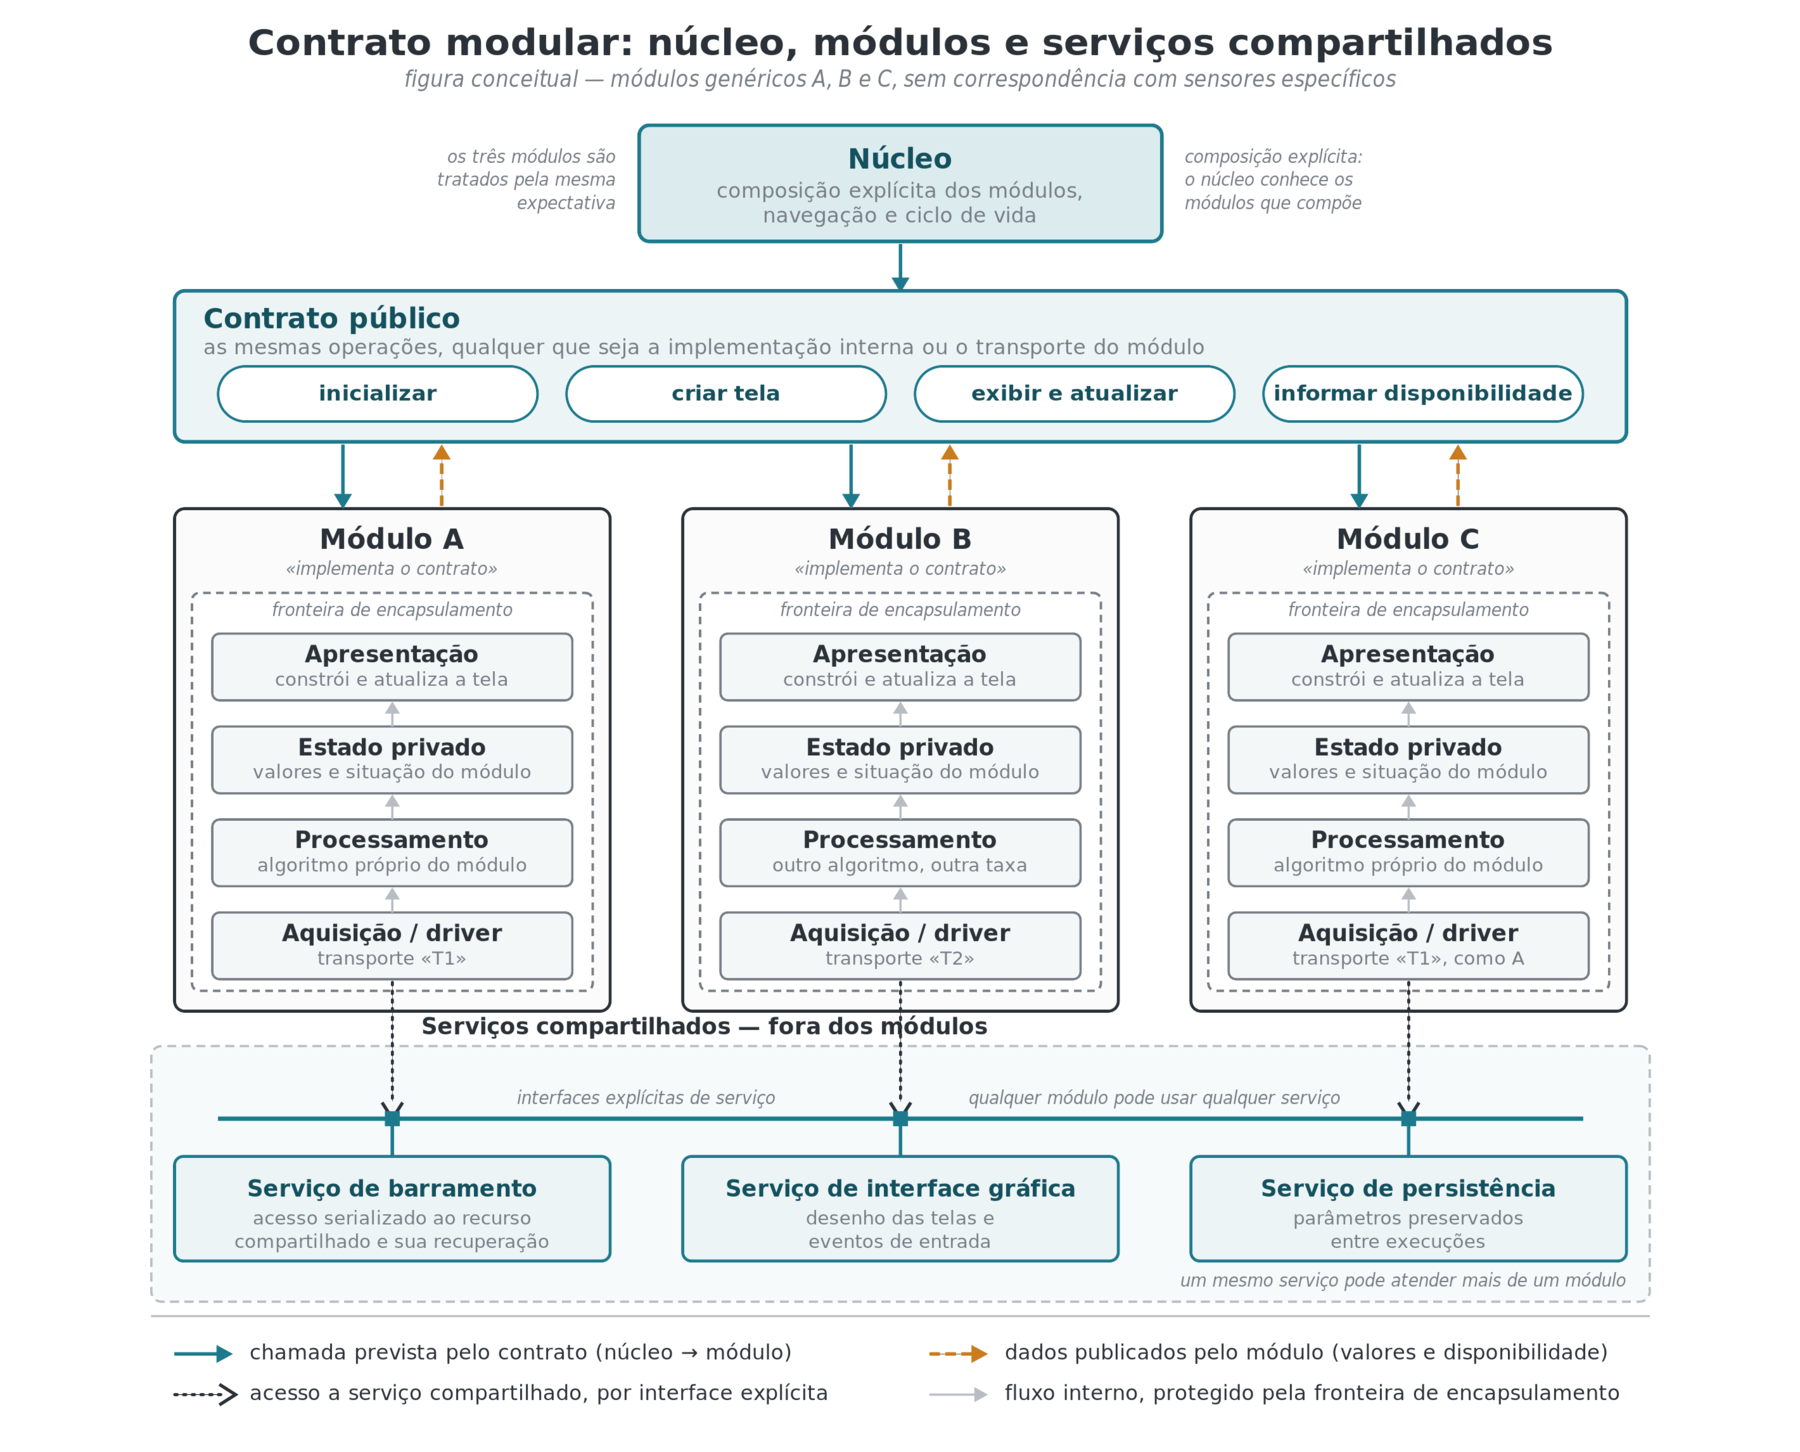
\includegraphics[width=0.96\textwidth]{contrato_modular.png}
\begin{minipage}{0.96\textwidth}
\fonteelemento{Elaborado pelo autor com base em Parnas (1972) e Meyer (1992)}
\end{minipage}
\end{figure}


O ciclo de vida de um m\'odulo pode compreender inicializa\c{c}\~ao, ativa\c{c}\~ao, opera\c{c}\~ao, desativa\c{c}\~ao e libera\c{c}\~ao de recursos. O contrato precisa distinguir um m\'odulo ainda n\~ao inicializado, dispon\'ivel, temporariamente indispon\'ivel ou em falha, de modo que chamadas fora do estado permitido possam ser rejeitadas de forma previs\'ivel. A inicializa\c{c}\~ao n\~ao fatal \'e uma pol\'itica arquitetural em que a indisponibilidade de uma fun\c{c}\~ao opcional \'e registrada e isolada, permitindo prosseguir com fun\c{c}\~oes sem depend\^encia daquele recurso.


\subsubsection{Separa\c{c}\~ao de responsabilidades}


Em firmware, uma decomposi\c{c}\~ao recorrente separa a adapta\c{c}\~ao ao hardware, o driver do dispositivo, o processamento do sinal, a tarefa de coordena\c{c}\~ao e a apresenta\c{c}\~ao. A camada de abstra\c{c}\~ao de hardware (Hardware Abstraction Layer --- HAL) representa capacidades do perif\'erico do microcontrolador; o driver traduz registradores e transa\c{c}\~oes do componente; o processamento transforma amostras em grandezas ou eventos; a tarefa define quando adquirir e publicar; e a apresenta\c{c}\~ao transforma o estado em elementos da interface.


Essa separa\c{c}\~ao reduz a propaga\c{c}\~ao de detalhes, mas n\~ao cria independ\^encia absoluta. Um algoritmo continua condicionado pela taxa de amostragem e pela faixa configuradas no hardware, e uma tela continua condicionada \`a disponibilidade e \`a validade dos dados. Em sistemas restritos, interfaces adicionais, c\'opias de dados e estados intermedi\'arios tamb\'em consomem mem\'oria e tempo. A abstra\c{c}\~ao deve preservar depend\^encias relevantes e ocultar apenas as decis\~oes que n\~ao precisam atravessar a fronteira do m\'odulo.


\subsubsection{Extensibilidade}


Extensibilidade \'e a capacidade de incorporar novas fun\c{c}\~oes ou ampliar fun\c{c}\~oes existentes com impacto controlado sobre a arquitetura. Ela n\~ao pode ser inferida apenas da exist\^encia de diret\'orios ou fun\c{c}\~oes separados. Sua avalia\c{c}\~ao requer um cen\'ario de mudan\c{c}a que identifique o est\'imulo, a parte modificada, as condi\c{c}\~oes da altera\c{c}\~ao e uma medida de resposta, como n\'umero de m\'odulos afetados, interfaces modificadas ou esfor\c{c}o necess\'ario (BASS; CLEMENTS; KAZMAN, 2021).


A extensibilidade depende das decis\~oes tomadas antecipadamente sobre pontos de varia\c{c}\~ao. Interfaces est\'aveis, responsabilidades localizadas e servi\c{c}os comuns reduzem a necessidade de repetir c\'odigo ou alterar o n\'ucleo a cada inclus\~ao. Entretanto, mecanismos gen\'ericos tamb\'em possuem custo de mem\'oria, processamento e complexidade. Em sistemas com recursos restritos, a arquitetura deve oferecer os pontos de extens\~ao necess\'arios ao problema sem introduzir abstra\c{c}\~oes cujo custo n\~ao seja justificado.


A demonstra\c{c}\~ao de extensibilidade deve observar uma modifica\c{c}\~ao concreta. A adi\c{c}\~ao de um novo m\'odulo, por exemplo, permite registrar quais arquivos e interfaces precisaram mudar e se m\'odulos existentes permaneceram inalterados. Esse procedimento produz evid\^encia mais direta do que a classifica\c{c}\~ao da arquitetura com base apenas em sua estrutura declarada.


\subsubsection{Toler\^ancia a falhas e continuidade das fun\c{c}\~oes independentes}


Na terminologia de dependabilidade, uma falha interna pode produzir um estado incorreto e, caso esse estado alcance a interface do sistema, resultar na interrup\c{c}\~ao ou na presta\c{c}\~ao incorreta de um servi\c{c}o. A toler\^ancia a falhas compreende os meios empregados para evitar que a presen\c{c}a de uma falha provoque a falha do servi\c{c}o oferecido (AVIZIENIS et al., 2004). Essa propriedade n\~ao equivale \`a impossibilidade de falhas nem garante, isoladamente, confiabilidade absoluta.


Em uma plataforma composta por fun\c{c}\~oes independentes, a falha ou aus\^encia de um sensor n\~ao precisa impedir a inicializa\c{c}\~ao dos demais m\'odulos. Para isso, a arquitetura deve conter o erro no subsistema afetado, comunicar sua indisponibilidade e preservar os servi\c{c}os que n\~ao dependem dele. A continuidade obtida est\'a limitada pelas depend\^encias reais: a falha de um recurso compartilhado pode afetar v\'arios m\'odulos e exige mecanismos espec\'ificos de coordena\c{c}\~ao, detec\c{c}\~ao e recupera\c{c}\~ao.


Esse comportamento deve ser avaliado pela introdu\c{c}\~ao controlada de falhas e pela observa\c{c}\~ao dos servi\c{c}os preservados. Ensaios com sensores ausentes, erros de comunica\c{c}\~ao e recupera\c{c}\~ao de recursos compartilhados permitem distinguir uma decis\~ao arquitetural implementada de uma propriedade efetivamente demonstrada.


\subsection{Sistemas operacionais de tempo real}


Um sistema operacional de tempo real (Real-Time Operating System --- RTOS) organiza a execu\c{c}\~ao de atividades concorrentes de acordo com requisitos temporais. Seu objetivo n\~ao \'e apenas executar opera\c{c}\~oes rapidamente, mas oferecer comportamento temporal suficientemente previs\'ivel para que eventos sejam tratados dentro dos limites definidos pela aplica\c{c}\~ao. Esses limites podem assumir a forma de per\'iodos de ativa\c{c}\~ao, prazos, lat\^encias m\'aximas ou tempos de resposta.


Em um sistema embarcado multissensor, o uso de um sistema operacional de tempo real permite representar aquisi\c{c}\~oes, processamento e interface como tarefas separadas. Essa decomposi\c{c}\~ao facilita a atribui\c{c}\~ao de per\'iodos e prioridades, mas n\~ao garante por si s\'o que os requisitos temporais sejam atendidos. O tempo de execu\c{c}\~ao das tarefas, as rela\c{c}\~oes de preced\^encia, o compartilhamento de recursos e os intervalos em que interrup\c{c}\~oes ou regi\~oes cr\'iticas impedem o escalonamento tamb\'em afetam o comportamento do sistema.


\subsubsection{Tarefas e escalonamento}


Uma tarefa representa um fluxo de execu\c{c}\~ao com contexto e pilha pr\'oprios. Durante sua exist\^encia, ela transita entre estados controlados pelo n\'ucleo: pode estar em execu\c{c}\~ao, pronta para executar, bloqueada \`a espera de tempo ou evento, ou suspensa explicitamente. Uma tarefa bloqueada n\~ao disputa o processador at\'e que sua condi\c{c}\~ao de desbloqueio seja satisfeita, o que permite aguardar per\'iodos, filas, notifica\c{c}\~oes ou recursos sem executar espera ocupada (FREERTOS, 2026a).


Em um escalonador preemptivo baseado em prioridades, a tarefa pronta de maior prioridade recebe o processador. Quando uma tarefa de prioridade superior se torna pronta, ela pode interromper a execu\c{c}\~ao de uma tarefa menos priorit\'aria. Tarefas de mesma prioridade podem compartilhar o processador por altern\^ancia temporal quando essa op\c{c}\~ao est\'a habilitada. A escolha das prioridades deve refletir requisitos de resposta e depend\^encias, pois atribuir prioridade elevada a uma atividade que executa continuamente pode impedir o progresso das demais.


O escalonamento de tarefas peri\'odicas \'e um problema cl\'assico de sistemas de tempo real. Liu e Layland (1973) demonstraram condi\c{c}\~oes de escalonabilidade para conjuntos de tarefas peri\'odicas independentes sob algoritmos de prioridade fixa e din\^amica. As hip\'oteses desses modelos, como independ\^encia entre tarefas e conhecimento de seus piores tempos de execu\c{c}\~ao, n\~ao s\~ao automaticamente satisfeitas em um firmware que compartilha barramentos e mutexes. Por isso, prioridades e per\'iodos precisam ser analisados em conjunto com os bloqueios introduzidos pela sincroniza\c{c}\~ao.


Em muitos sistemas operacionais de tempo real, um temporizador gera interrup\c{c}\~oes peri\'odicas denominadas \emph{ticks}. A cada ocorr\^encia, o n\'ucleo atualiza sua refer\^encia de tempo, verifica atrasos e limites de espera e pode liberar tarefas bloqueadas. A frequ\^encia do \emph{tick} determina a resolu\c{c}\~ao temporal dessas opera\c{c}\~oes: uma frequ\^encia mais alta oferece granularidade mais fina, mas aumenta a quantidade de interrup\c{c}\~oes executadas pelo n\'ucleo. Uma frequ\^encia mais baixa reduz essa sobrecarga, por\'em limita a resolu\c{c}\~ao dos atrasos expressos em m\'ultiplos de \emph{ticks}. Para tarefas peri\'odicas, atrasos relativos sucessivos podem acumular varia\c{c}\~ao de fase; mecanismos que utilizam como refer\^encia o instante de libera\c{c}\~ao anterior permitem manter um per\'iodo mais regular. Essa diferen\c{c}a temporal \'e representada na Figura~\ref{fig:tick-atrasos}.


\begin{figure}[H]
\centering
\caption{Diferen\c{c}a conceitual entre atrasos relativos e refer\^encia temporal peri\'odica}
\label{fig:tick-atrasos}
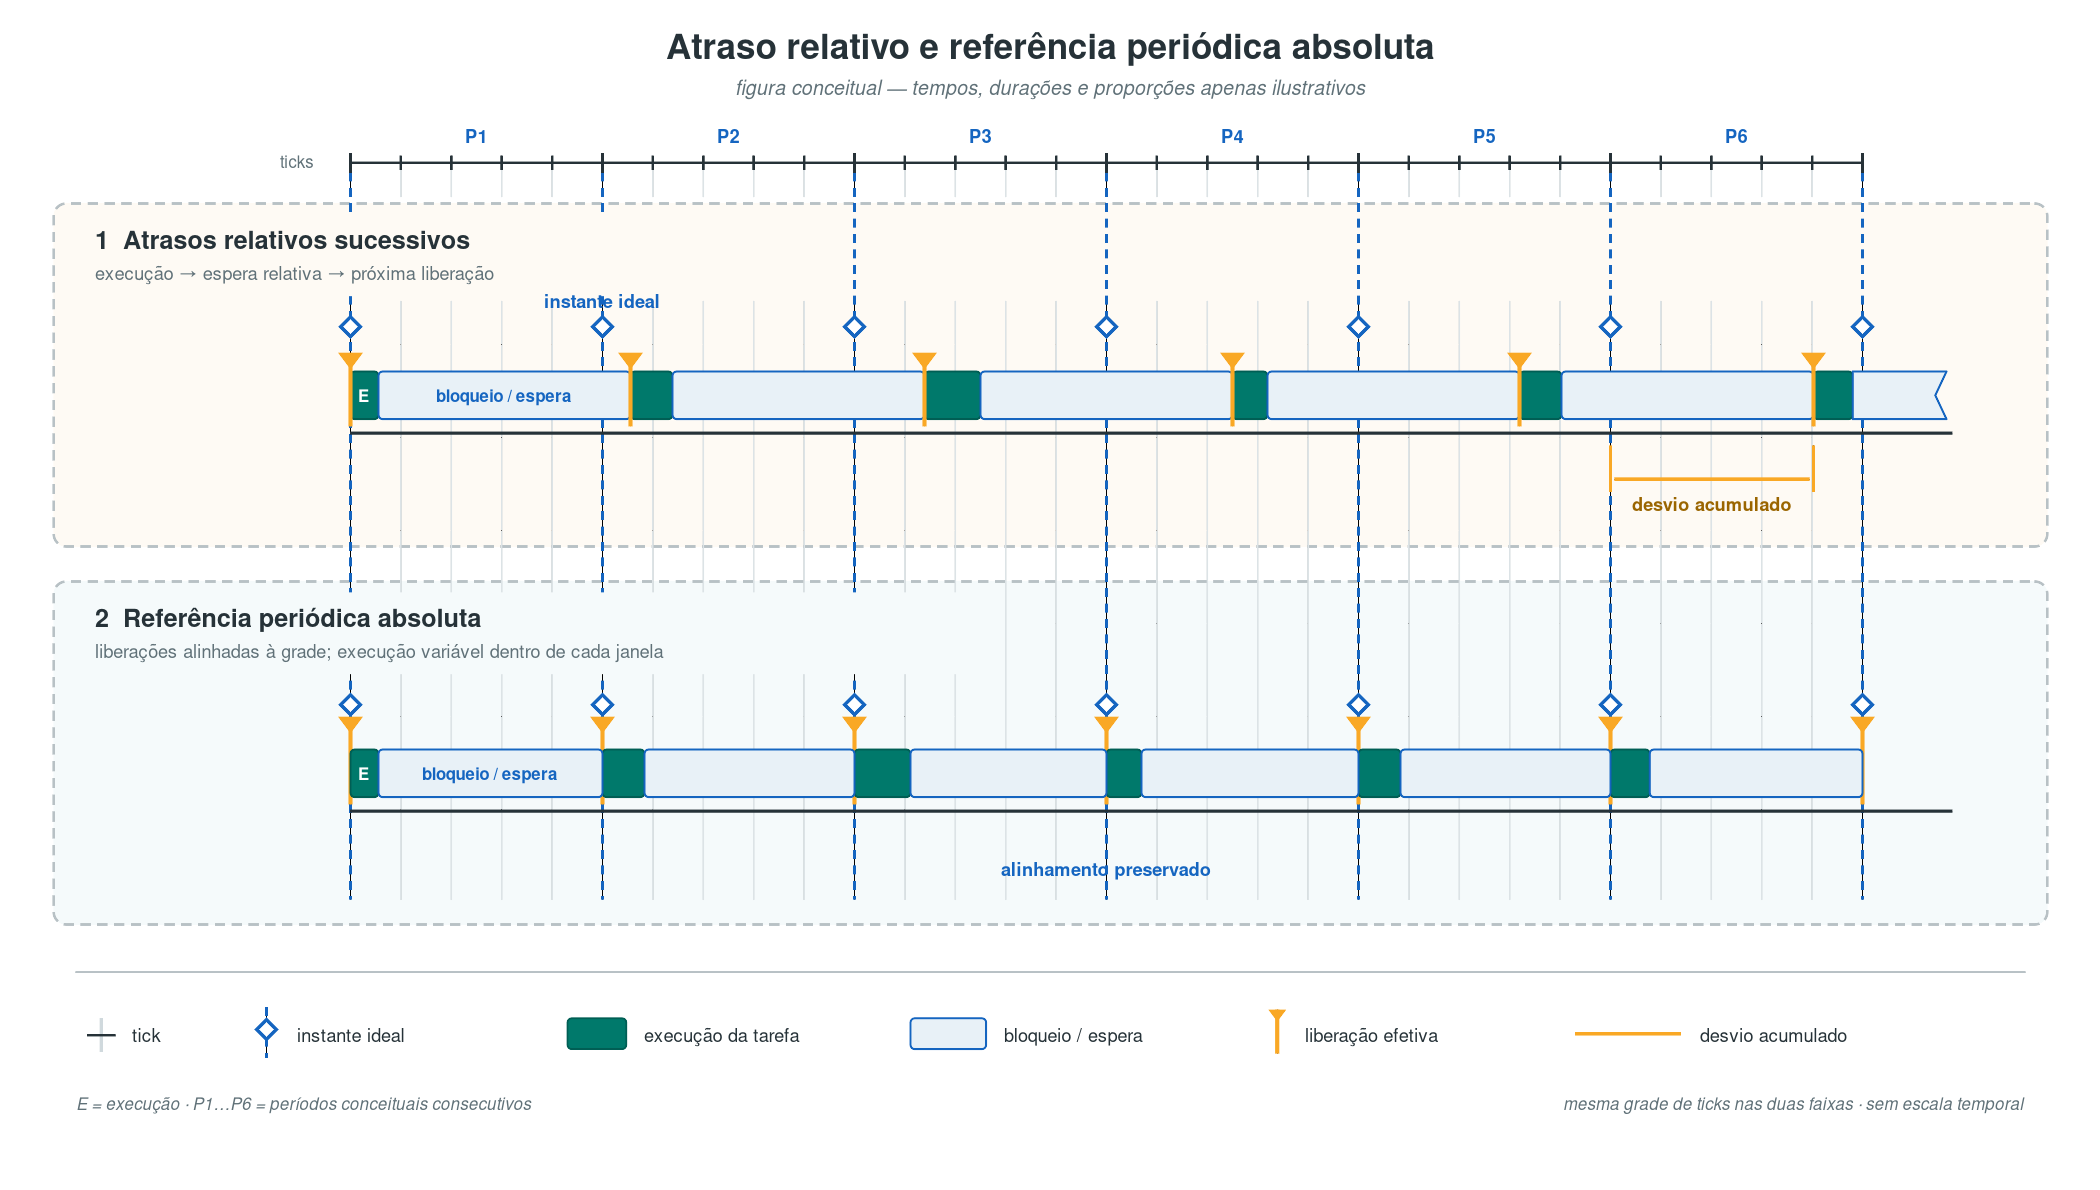
\includegraphics[width=0.94\textwidth]{tick_atrasos.png}
\fonteelemento{Elaborado pelo autor com base na documenta\c{c}\~ao do FreeRTOS (2026a)}
\end{figure}


\subsubsection{Sincroniza\c{c}\~ao e exclus\~ao m\'utua}


Tarefas concorrentes podem acessar dados ou recursos cuja utiliza\c{c}\~ao precisa ser coordenada. Sem sincroniza\c{c}\~ao, o resultado pode depender da ordem das opera\c{c}\~oes, produzindo condi\c{c}\~oes de corrida, estados parcialmente atualizados ou transa\c{c}\~oes sobrepostas. A necessidade de prote\c{c}\~ao depende tanto da atomicidade oferecida pelo processador quanto da sequ\^encia l\'ogica que deve permanecer indivis\'ivel.


A exclus\~ao m\'utua permite que somente uma tarefa por vez execute uma regi\~ao associada a um recurso compartilhado. O objeto de exclus\~ao m\'utua (mutex) possui rela\c{c}\~ao de propriedade: a tarefa que o obt\'em deve liber\'a-lo depois de concluir o acesso protegido. Essa caracter\'istica o diferencia de mecanismos usados apenas para sinaliza\c{c}\~ao de eventos. No FreeRTOS, mutexes incluem heran\c{c}a de prioridade, enquanto sem\'aforos bin\'arios n\~ao oferecem esse mecanismo (FREERTOS, 2026b).


O tempo durante o qual um mutex permanece retido afeta a lat\^encia das tarefas concorrentes. A regi\~ao protegida deve conter somente as opera\c{c}\~oes que precisam ser serializadas, sem atrasos deliberados ou processamento alheio ao recurso. Quando uma opera\c{c}\~ao de entrada e sa\'ida requer v\'arias etapas para preservar a integridade de uma transa\c{c}\~ao, liberar a prote\c{c}\~ao entre essas etapas pode permitir interfer\^encia de outra tarefa, ainda que reduza aparentemente o tempo de bloqueio.


O uso de v\'arios recursos protegidos tamb\'em pode criar espera circular. Se duas tarefas obt\^em mutexes em ordens diferentes, cada uma pode reter um recurso enquanto aguarda o outro. Uma ordem global de aquisi\c{c}\~ao, a redu\c{c}\~ao do aninhamento e o tratamento expl\'icito de limites de espera s\~ao medidas de projeto para evitar ou detectar esse bloqueio.


\subsubsection{\texttt{volatile}, atomicidade e sincroniza\c{c}\~ao}


Na linguagem C, o qualificador \texttt{volatile} obriga o compilador a preservar acessos observ\'aveis ao objeto segundo as regras da linguagem, sendo pertinente quando o valor pode mudar por uma interrup\c{c}\~ao ou por hardware mapeado em mem\'oria. Ele n\~ao torna uma sequ\^encia de leitura, modifica\c{c}\~ao e escrita indivis\'ivel, n\~ao estabelece propriedade de um recurso e n\~ao substitui mutexes, regi\~oes cr\'iticas ou primitivas at\^omicas.


Mesmo quando uma leitura ou escrita alinhada cabe em uma instru\c{c}\~ao do processador, uma opera\c{c}\~ao composta pode sofrer interfer\^encia entre suas etapas. Al\'em disso, a corre\c{c}\~ao depende da ordena\c{c}\~ao e da visibilidade exigidas entre tarefas e interrup\c{c}\~oes. Portanto, a escolha da primitiva deve decorrer do invariante a proteger, e n\~ao apenas do tamanho da vari\'avel compartilhada.


\subsubsection{Invers\~ao de prioridade e heran\c{c}a}


A invers\~ao de prioridade ocorre quando uma tarefa de alta prioridade precisa aguardar um recurso retido por uma tarefa de prioridade inferior. O bloqueio pelo tempo necess\'ario \`a conclus\~ao da regi\~ao cr\'itica \'e inerente ao compartilhamento do recurso. O problema torna-se mais grave quando tarefas de prioridade intermedi\'aria, que n\~ao utilizam esse recurso, preemptam a tarefa que o ret\'em e prolongam indiretamente a espera da tarefa priorit\'aria.


No protocolo de heran\c{c}a de prioridade, a tarefa que ret\'em o recurso recebe temporariamente a maior prioridade entre as tarefas bloqueadas por ela. Isso permite que conclua a regi\~ao cr\'itica e libere o recurso sem ser sucessivamente preemptada por tarefas intermedi\'arias. Ap\'os a libera\c{c}\~ao, sua prioridade retorna ao valor anterior. Sha, Rajkumar e Lehoczky (1990) formalizaram protocolos destinados a limitar a invers\~ao de prioridade em sistemas de tempo real.


A heran\c{c}a reduz a invers\~ao n\~ao controlada, mas n\~ao elimina a necessidade de limitar regi\~oes cr\'iticas, definir uma ordem de aquisi\c{c}\~ao e analisar bloqueios encadeados. Tamb\'em n\~ao deve ser presumida para qualquer primitiva de sincroniza\c{c}\~ao: sua presen\c{c}a depende do tipo de objeto e da implementa\c{c}\~ao do sistema operacional. A Figura~\ref{fig:inversao-prioridade} compara o encadeamento sem heran\c{c}a com a eleva\c{c}\~ao tempor\'aria da prioridade da tarefa que det\'em o mutex.


\begin{figure}[H]
\centering
\caption{Invers\~ao de prioridade e efeito da heran\c{c}a sobre o bloqueio}
\label{fig:inversao-prioridade}
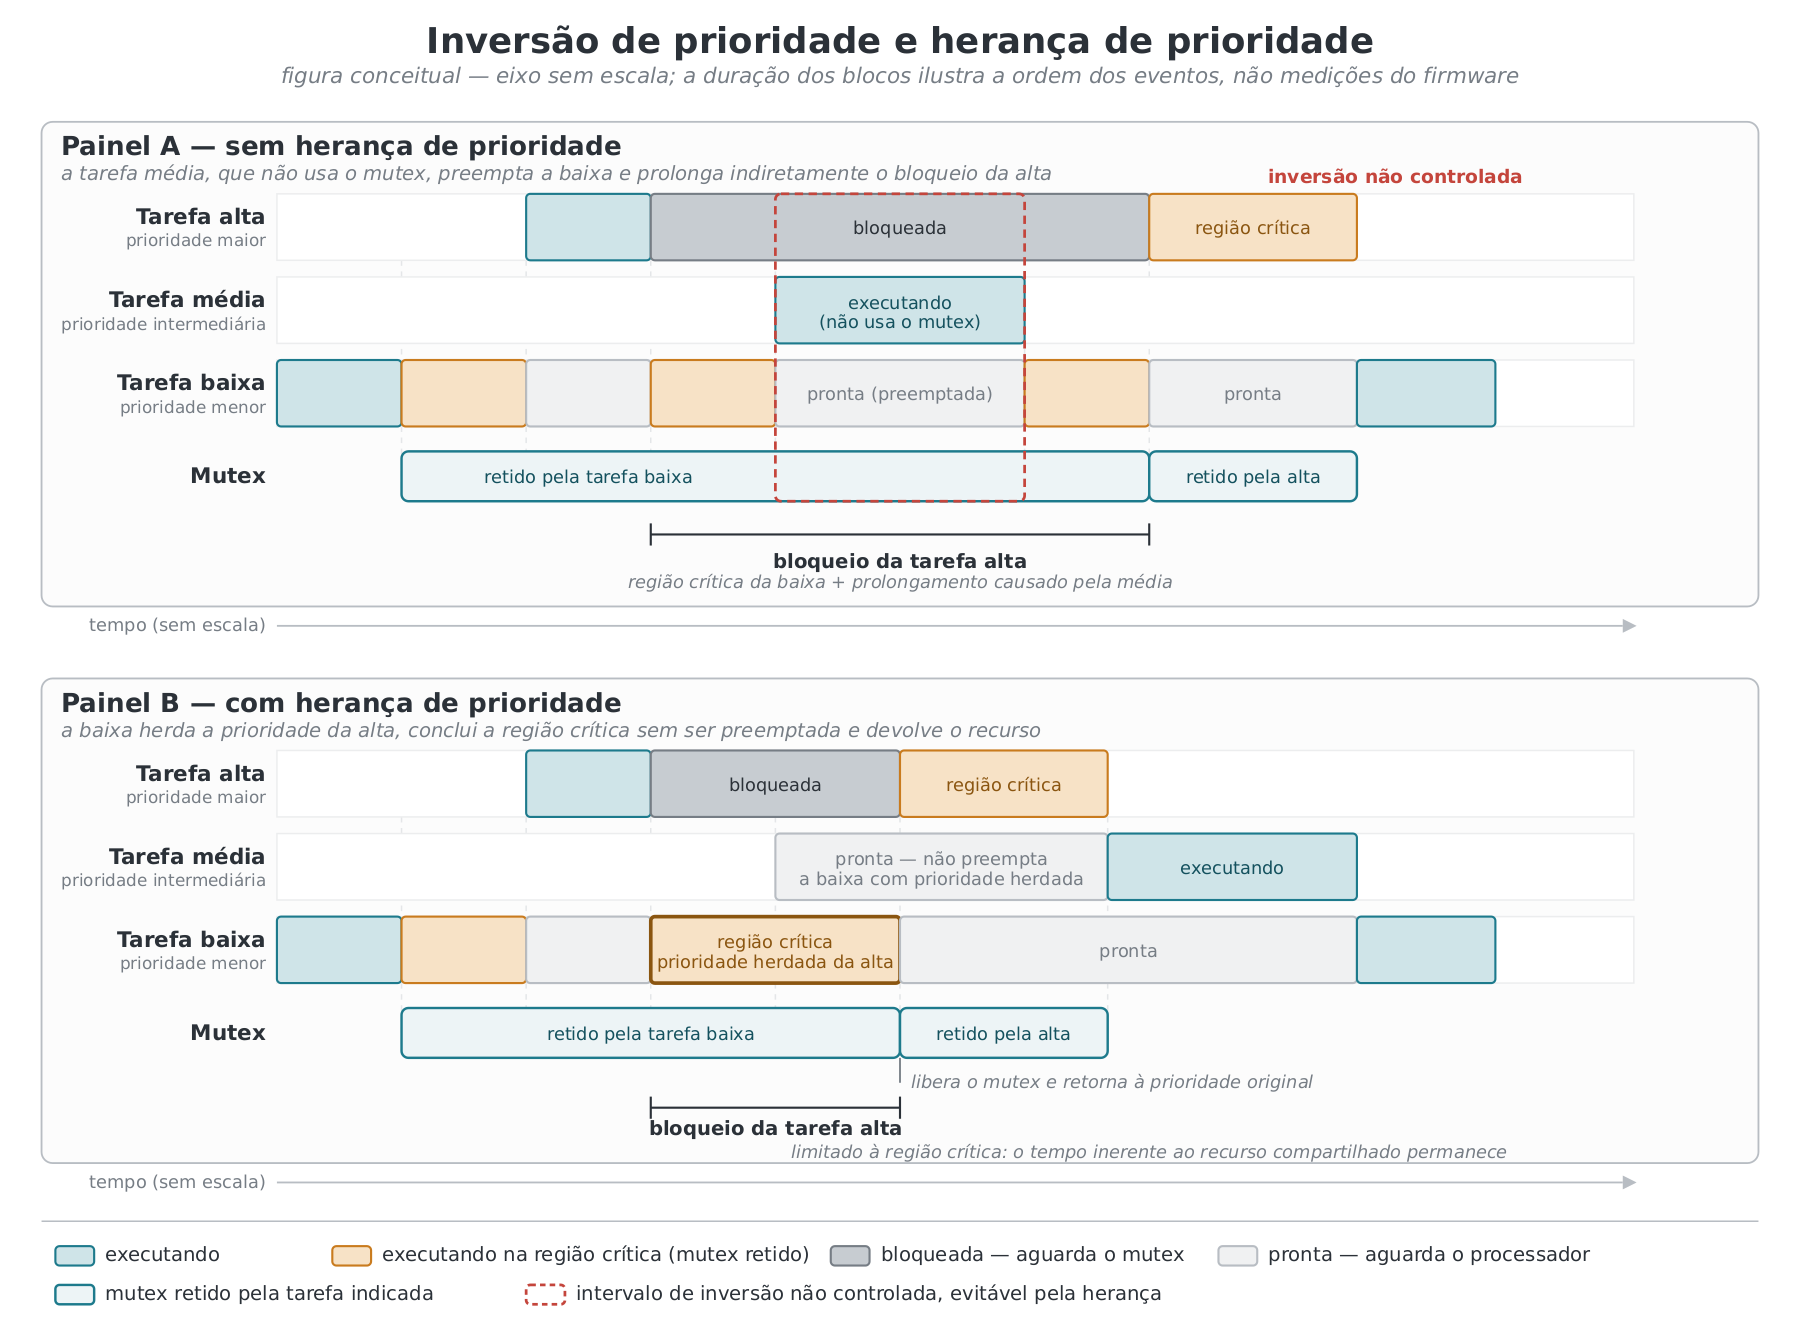
\includegraphics[width=0.94\textwidth]{inversao_prioridade.png}
\fonteelemento{Elaborado pelo autor com base em Sha, Rajkumar e Lehoczky (1990)}
\end{figure}


\subsubsection{Watchdog e carga do processador}


Um temporizador de supervis\~ao, ou \emph{watchdog}, detecta situa\c{c}\~oes em que uma parte do sistema deixa de progredir dentro de um intervalo estabelecido. No ESP-IDF, o watchdog de interrup\c{c}\~oes verifica per\'iodos prolongados em que as interrup\c{c}\~oes e a troca de tarefas n\~ao conseguem ocorrer, enquanto o watchdog de tarefas pode monitorar tarefas inscritas e a execu\c{c}\~ao da tarefa ociosa. A aus\^encia prolongada de execu\c{c}\~ao da tarefa ociosa \'e um ind\'icio de que alguma tarefa n\~ao est\'a cedendo o processador (ESPRESSIF SYSTEMS, 2025d).


O disparo de um watchdog identifica uma viola\c{c}\~ao temporal, mas n\~ao determina sozinho sua causa. Regi\~oes cr\'iticas extensas, interrup\c{c}\~oes desabilitadas, espera ocupada, processamento excessivo e opera\c{c}\~oes longas sobre mem\'oria n\~ao vol\'atil podem produzir sintomas semelhantes. O limite de supervis\~ao deve ser compat\'ivel com o maior intervalo leg\'itimo de execu\c{c}\~ao, sem ser ampliado apenas para ocultar tarefas que deixam de bloquear ou ceder o processador.


A carga da unidade central de processamento (Central Processing Unit --- CPU) pode ser estimada pelo tempo durante o qual as tarefas permanecem em execu\c{c}\~ao. O FreeRTOS pode acumular estat\'isticas de tempo de execu\c{c}\~ao por tarefa e apresent\'a-las como valores absolutos e percentuais, desde que seja configurada uma base de tempo com resolu\c{c}\~ao adequada (FREERTOS, 2026c). Em uma plataforma de n\'ucleo \'unico, o tempo atribu\'ido \`a tarefa ociosa tamb\'em permite estimar a parcela n\~ao utilizada do processador.


Essas m\'etricas dependem da janela de observa\c{c}\~ao e do estado funcional da aplica\c{c}\~ao. Uma medi\c{c}\~ao realizada com telas est\'aticas ou sensores inativos n\~ao representa necessariamente o pior caso. A coleta de estat\'isticas tamb\'em introduz custo de instrumenta\c{c}\~ao, e o percentual de CPU n\~ao substitui a verifica\c{c}\~ao de lat\^encias e prazos das tarefas cr\'iticas.


Uma estimativa baseada na execu\c{c}\~ao da tarefa ociosa pode indicar a folga global do processador em uma janela, desde que exista uma refer\^encia obtida sob condi\c{c}\~oes equivalentes. Ela n\~ao atribui custo a cada tarefa, n\~ao revela diretamente bloqueios em barramentos e pode variar com interrup\c{c}\~oes, modos funcionais e instrumenta\c{c}\~ao. O \emph{idle hook} deve executar rapidamente e n\~ao pode conter espera bloqueante, pois \'e chamado no contexto da tarefa ociosa (FREERTOS, 2026c).


\subsection{Interfaces de comunica\c{c}\~ao}


Interfaces seriais transferem dados por um n\'umero reduzido de condutores, em contraste com interfaces paralelas que transportam v\'arios bits simultaneamente. A quantidade de sinais, o m\'etodo de endere\c{c}amento, a forma de sincroniza\c{c}\~ao e os mecanismos de confirma\c{c}\~ao variam entre os protocolos. Em uma plataforma com sensores e interface gr\'afica, a escolha de cada interface afeta a ocupa\c{c}\~ao de pinos, a taxa de transfer\^encia, a complexidade el\'etrica e a coordena\c{c}\~ao do acesso por software.


\subsubsection{I$^2$C}


O barramento Inter-Integrated Circuit (I$^2$C) utiliza duas linhas: dados seriais (Serial Data --- SDA) e clock serial (Serial Clock --- SCL). As linhas empregam sa\'idas de dreno aberto ou coletor aberto e resistores de \emph{pull-up}. Os dispositivos conectados podem for\c{c}ar uma linha ao n\'ivel baixo, mas o n\'ivel alto resulta da libera\c{c}\~ao coletiva da linha e da a\c{c}\~ao dos resistores. Essa caracter\'istica permite compartilhar os mesmos condutores sem que duas sa\'idas ativas imponham n\'iveis l\'ogicos opostos (NXP SEMICONDUCTORS, 2021).


A comunica\c{c}\~ao \'e organizada em transa\c{c}\~oes iniciadas por uma condi\c{c}\~ao de START e encerradas por uma condi\c{c}\~ao de STOP ou por um START repetido. Ap\'os o endere\c{c}o e a indica\c{c}\~ao de leitura ou escrita, os dados s\~ao transmitidos em grupos de oito bits. Cada byte \'e seguido por um bit de reconhecimento: ACK indica que o receptor reconheceu a transfer\^encia, enquanto NACK pode sinalizar aus\^encia do dispositivo, impossibilidade de receber mais dados ou t\'ermino de uma leitura, conforme a etapa da transa\c{c}\~ao.


V\'arios dispositivos podem compartilhar SDA e SCL, desde que seus endere\c{c}os n\~ao entrem em conflito e que as caracter\'isticas el\'etricas permane\c{c}am dentro dos limites do barramento. O tempo de subida depende da resist\^encia de \emph{pull-up} e da capacit\^ancia total do barramento, formada por dispositivos, trilhas, fios e conectores. O aumento da capacit\^ancia torna as transi\c{c}\~oes para o n\'ivel alto mais lentas e pode limitar a frequ\^encia utiliz\'avel, sendo necess\'ario dimensionar o resistor de \emph{pull-up} de modo a atender simultaneamente ao tempo m\'aximo de subida e \`a corrente que os dispositivos devem drenar quando a linha est\'a em n\'ivel baixo. A Figura~\ref{fig:i2c-open-drain} relaciona o comportamento de dreno aberto \`a subida determinada pela rede resistivo-capacitiva.


\begin{figure}[H]
\centering
\caption{Linha I$^2$C em dreno aberto e subida determinada pela rede de \emph{pull-up} e pela capacit\^ancia equivalente}
\label{fig:i2c-open-drain}
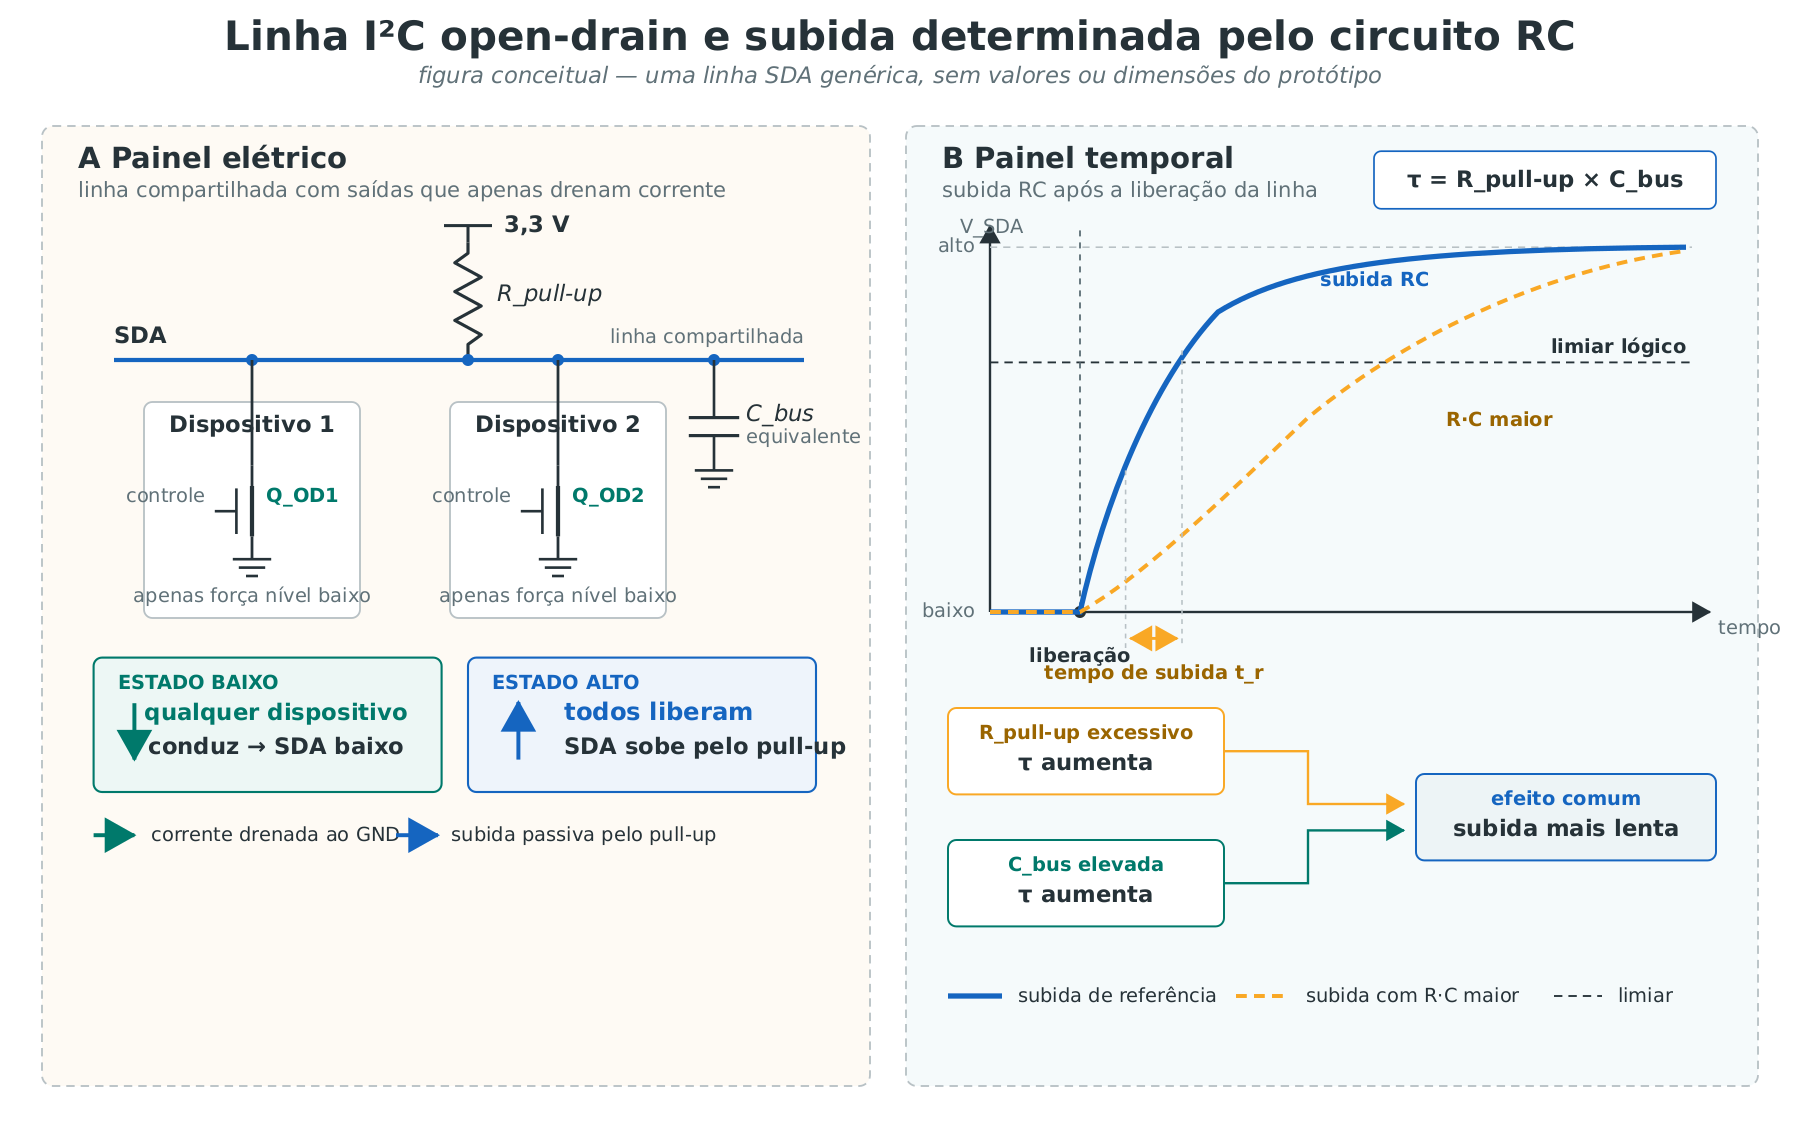
\includegraphics[width=0.94\textwidth]{i2c_open_drain_rc.png}
\fonteelemento{Elaborado pelo autor com base em NXP Semiconductors (2021)}
\end{figure}


O protocolo tamb\'em prev\^e arbitragem para situa\c{c}\~oes em que mais de um controlador pode iniciar transfer\^encias. Alguns dispositivos podem prolongar o n\'ivel baixo de SCL para adiar a continua\c{c}\~ao da transa\c{c}\~ao, recurso denominado \emph{clock stretching}. O suporte efetivo a esses recursos depende dos controladores e dispositivos empregados.


O compartilhamento f\'isico n\~ao fornece exclus\~ao m\'utua entre tarefas de software. Quando diferentes tarefas iniciam transa\c{c}\~oes pelo mesmo controlador, o driver ou a aplica\c{c}\~ao deve preservar a atomicidade de cada opera\c{c}\~ao e impedir que sequ\^encias pertencentes a dispositivos distintos sejam intercaladas. Erros como NACK, limite de espera e barramento ocupado precisam ser tratados de acordo com o estado reportado pelo controlador.


A especifica\c{c}\~ao define, entre outros, o modo padr\~ao de at\'e 100 kbit/s e o modo r\'apido de at\'e 400 kbit/s (NXP SEMICONDUCTORS, 2021). Operar a 100 kbit/s em uma integra\c{c}\~ao e a 400 kbit/s em um teste isolado constitui uma decis\~ao de configura\c{c}\~ao condicionada pelos dispositivos, pela interliga\c{c}\~ao e pelas margens temporais; n\~ao implica que uma das frequ\^encias seja universalmente correta. Ap\'os falhas, a recupera\c{c}\~ao pode exigir encerrar ou reinicializar a transa\c{c}\~ao e o controlador, ou liberar uma linha retida segundo as capacidades do hardware. A estrat\'egia deve evitar que uma tentativa local de recupera\c{c}\~ao interfira em outra transa\c{c}\~ao v\'alida no mesmo barramento.


\subsubsection{SPI}


A Serial Peripheral Interface (SPI) \'e uma interface serial s\'incrona na qual um controlador fornece o sinal de clock e seleciona o dispositivo participante da transa\c{c}\~ao. Na configura\c{c}\~ao convencional, s\~ao utilizados o clock serial (Serial Clock --- SCLK), a linha de dados do controlador para o perif\'erico (Master Out, Slave In --- MOSI), a linha de retorno (Master In, Slave Out --- MISO) e um sinal de sele\c{c}\~ao, usualmente denominado Chip Select (CS), para cada dispositivo.


Como MOSI e MISO s\~ao linhas distintas, a transfer\^encia pode ocorrer simultaneamente nas duas dire\c{c}\~oes. Aplica\c{c}\~oes que necessitam apenas de escrita ou apenas de leitura podem omitir uma das linhas. Diferentemente do I$^2$C, a forma convencional de SPI n\~ao inclui endere\c{c}amento no barramento nem um bit padronizado de reconhecimento a cada byte. O significado dos bits transferidos, a organiza\c{c}\~ao de comandos e a indica\c{c}\~ao de erros s\~ao definidos pelo protocolo do dispositivo.


A rela\c{c}\~ao entre a polaridade do clock e a borda usada para lan\c{c}ar ou amostrar os dados determina o modo SPI. Controlador e perif\'erico precisam utilizar combina\c{c}\~oes compat\'iveis de polaridade e fase; uma configura\c{c}\~ao incorreta pode deslocar a amostragem e corromper os dados. Tamb\'em devem ser respeitados os tempos de ativa\c{c}\~ao do CS, propaga\c{c}\~ao e prepara\c{c}\~ao especificados para o perif\'erico.


Dispositivos podem compartilhar SCLK, MOSI e MISO, permanecendo inativos enquanto seus sinais CS n\~ao estiverem selecionados. Cada dispositivo adicional normalmente exige uma linha CS pr\'opria. O controlador precisa impedir a sobreposi\c{c}\~ao de transa\c{c}\~oes e aplicar a configura\c{c}\~ao de clock e modo correspondente ao dispositivo selecionado. No driver mestre do ESP-IDF, uma transa\c{c}\~ao compreende a sele\c{c}\~ao por CS, a transfer\^encia e a libera\c{c}\~ao do dispositivo; o driver tamb\'em pode utilizar acesso direto \`a mem\'oria para transferir blocos sem movimentar cada byte diretamente pela CPU (ESPRESSIF SYSTEMS, 2025e).


\subsubsection{1-Wire}


O 1-Wire \'e um protocolo serial bidirecional que utiliza uma linha de dados, al\'em da refer\^encia de terra, para comunica\c{c}\~ao entre um controlador e um ou mais dispositivos. A linha \'e compartilhada e mantida em n\'ivel alto por um resistor de \emph{pull-up}; controlador e dispositivos sinalizam ao for\c{c}\'a-la temporariamente ao n\'ivel baixo. Alguns dispositivos podem obter energia da pr\'opria linha quando ela permanece em n\'ivel alto, modalidade denominada alimenta\c{c}\~ao parasita, enquanto outros admitem alimenta\c{c}\~ao externa (ANALOG DEVICES, 2008).


Uma comunica\c{c}\~ao come\c{c}a com um pulso de reinicializa\c{c}\~ao produzido pelo controlador. Os dispositivos presentes respondem com um pulso de presen\c{c}a, ap\'os o qual s\~ao transmitidos comandos de endere\c{c}amento e de fun\c{c}\~ao. Cada dispositivo possui um identificador de 64 bits, que permite selecionar uma unidade espec\'ifica, selecionar todas as unidades ou executar um procedimento de busca no barramento (ANALOG DEVICES, 2019).


Os bits s\~ao representados por intervalos temporais durante os quais o controlador e o dispositivo alteram ou amostram o n\'ivel da linha. H\'a intervalos distintos para escrita de zero, escrita de um e leitura, al\'em de tempos m\'inimos de recupera\c{c}\~ao. Como a interpreta\c{c}\~ao depende da dura\c{c}\~ao dos pulsos e do instante de amostragem, atrasos introduzidos pelo software ou por interrup\c{c}\~oes podem violar os limites do protocolo. No DS18B20, por exemplo, cada intervalo transporta um bit, e o controlador inicia todos os sinais, exceto o pulso de presen\c{c}a (ANALOG DEVICES, 2019).


A redu\c{c}\~ao do n\'umero de condutores ocorre em troca de menor taxa de transfer\^encia e de requisitos temporais estritos. A capacit\^ancia da linha, o valor do resistor de \emph{pull-up}, a topologia da conex\~ao e a quantidade de dispositivos influenciam os tempos de subida e a margem dispon\'ivel para amostragem.


\subsubsection{RMT}


O Remote Control Transceiver (RMT) \'e um perif\'erico para transmiss\~ao e recep\c{c}\~ao de sinais definidos por n\'iveis l\'ogicos e dura\c{c}\~oes. Embora tenha sido concebido para sinais de controle remoto por infravermelho, seu formato permite representar outros protocolos baseados em pulsos. Cada s\'imbolo associa dois n\'iveis a seus respectivos intervalos de dura\c{c}\~ao, e canais independentes podem ser configurados para transmiss\~ao ou recep\c{c}\~ao (ESPRESSIF SYSTEMS, 2025f).


O RMT n\~ao define endere\c{c}os, comandos ou regras de um protocolo de comunica\c{c}\~ao. Ele fornece os recursos temporais usados para produzir ou medir a forma de onda. Um codificador ou driver de n\'ivel superior continua respons\'avel por converter comandos e dados nos s\'imbolos correspondentes e por interpretar os pulsos recebidos.


Ao transferir a gera\c{c}\~ao e a medi\c{c}\~ao dos pulsos para um perif\'erico, reduz-se a depend\^encia de la\c{c}os de software executados com temporiza\c{c}\~ao precisa. Essa separa\c{c}\~ao \'e \'util quando o processador tamb\'em atende tarefas e interrup\c{c}\~oes que poderiam introduzir varia\c{c}\~ao nos instantes de altera\c{c}\~ao ou amostragem de uma entrada ou sa\'ida digital.


\subsection{Interface gr\'afica embarcada}


\subsubsection{TFT e RGB565}


Displays de transistores de filme fino (Thin-Film Transistor --- TFT) empregam uma matriz ativa para controlar os elementos da imagem. Em m\'odulos embarcados, um controlador integrado recebe comandos e dados de pixels, mant\'em a informa\c{c}\~ao na mem\'oria do display e atualiza a matriz. A aplica\c{c}\~ao n\~ao precisa transmitir continuamente o quadro completo para preservar uma imagem est\'atica, mas deve enviar os pixels correspondentes \`as regi\~oes que pretende modificar.


No formato RGB565, cada pixel \'e representado por 16 bits: cinco para vermelho, seis para verde e cinco para azul. Essa codifica\c{c}\~ao oferece \(2^{16}\), ou 65.536, combina\c{c}\~oes poss\'iveis e ocupa dois bytes por pixel. O canal verde recebe um bit adicional porque a sensibilidade visual n\~ao \'e igual para as tr\^es componentes. Em compara\c{c}\~ao com representa\c{c}\~oes de 24 ou 32 bits, o RGB565 reduz a mem\'oria e o volume transferido, com menor resolu\c{c}\~ao de cor (GALAXYCORE, 2022).


O tamanho de um quadro sem compress\~ao \'e dado pelo produto entre largura, altura e quantidade de bytes por pixel. Assim, a mem\'oria exigida cresce linearmente com a \'area da imagem e com a profundidade de cor. Em sistemas nos quais o quadro \'e enviado por uma interface serial, esses mesmos fatores tamb\'em afetam o tempo m\'inimo de transfer\^encia.


\subsubsection{Displays circulares}


Um display circular pode ser controlado por uma matriz de endere\c{c}amento retangular que cont\'em pixels n\~ao vis\'iveis nos cantos. A aplica\c{c}\~ao continua trabalhando com coordenadas cartesianas, mas somente os pontos internos \`a \'area circular aparecem ao usu\'ario. Para um display de raio \(r\) e centro \((x_c,y_c)\), um ponto \((x,y)\) pertence \`a regi\~ao vis\'ivel quando


\[
(x-x_c)^2+(y-y_c)^2 \leq r^2.
\]


Essa geometria reduz a largura dispon\'ivel nas partes superior e inferior da tela. Elementos adequados ao centro podem ser recortados quando deslocados para essas regi\~oes, ainda que suas coordenadas perten\c{c}am ao ret\^angulo l\'ogico. O projeto da interface deve considerar a extens\~ao completa de textos, imagens e \'areas sens\'iveis ao toque, e n\~ao apenas a posi\c{c}\~ao de seus centros.


O recorte circular tamb\'em influencia a organiza\c{c}\~ao visual. Indicadores perif\'ericos podem acompanhar a borda, enquanto informa\c{c}\~oes que exigem maior largura tendem a ocupar a faixa central. A transforma\c{c}\~ao entre coordenadas de toque e objetos gr\'aficos deve manter a mesma orienta\c{c}\~ao, origem e eventual rota\c{c}\~ao adotadas pelo controlador do display. A Figura~\ref{fig:display-circular} explicita a diferen\c{c}a entre a matriz l\'ogica quadrada, a regi\~ao circular vis\'ivel e a zona central conceitualmente mais segura.


\begin{figure}[H]
\centering
\caption{Geometria de uma \'area circular inscrita em uma matriz l\'ogica quadrada}
\label{fig:display-circular}
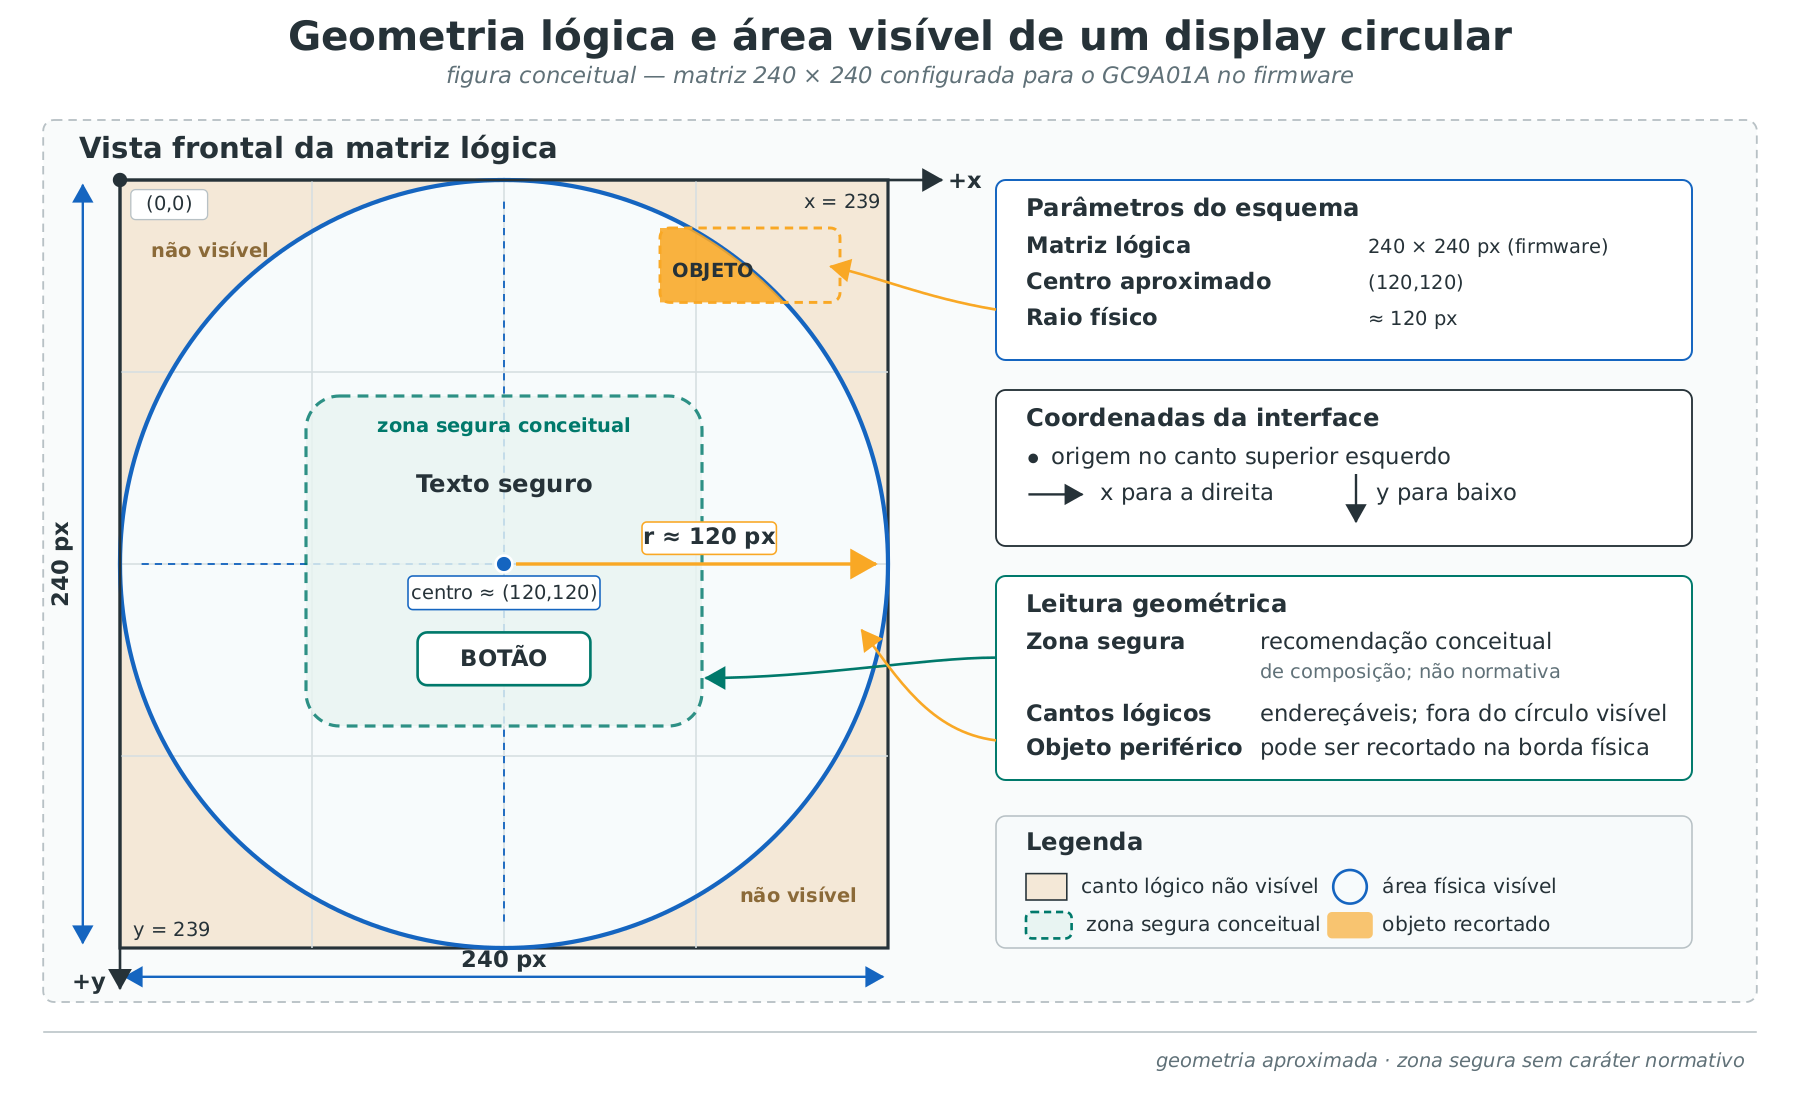
\includegraphics[width=0.90\textwidth]{display_circular_geometria.png}
\fonteelemento{Elaborado pelo autor}
\end{figure}


\subsubsection{LVGL e atualiza\c{c}\~ao parcial}


Bibliotecas gr\'aficas embarcadas, como a Light and Versatile Graphics Library (LVGL), representam a interface por objetos organizados hierarquicamente. Objetos podem conter outros objetos, herdar propriedades e responder a eventos. Essa organiza\c{c}\~ao separa a descri\c{c}\~ao da interface do mecanismo espec\'ifico usado para transferir pixels ao display (LVGL, 2023a).


Quando uma propriedade visual muda, a biblioteca marca como inv\'alidas as regi\~oes afetadas. Durante o ciclo de atualiza\c{c}\~ao, essas regi\~oes s\~ao combinadas quando conveniente, redesenhadas em um buffer e entregues ao driver por uma fun\c{c}\~ao de envio. Dessa forma, uma altera\c{c}\~ao localizada pode ser transmitida sem reconstruir e enviar necessariamente toda a tela (LVGL, 2023b).


O buffer de desenho pode corresponder ao quadro completo ou a uma fra\c{c}\~ao dele. Um buffer parcial reduz a mem\'oria reservada, mas pode exigir v\'arias etapas de desenho e transfer\^encia para concluir uma atualiza\c{c}\~ao. Buffers maiores diminuem a fragmenta\c{c}\~ao da opera\c{c}\~ao, enquanto dois buffers permitem que o processamento de uma regi\~ao se sobreponha \`a transfer\^encia de outra quando o hardware e o driver oferecem esse suporte. A escolha depende da mem\'oria dispon\'ivel, da taxa da interface e da complexidade da cena.


A atualiza\c{c}\~ao parcial reduz trabalho quando poucas regi\~oes mudam, mas seu efeito depende do conte\'udo. Anima\c{c}\~oes extensas, rolagem e objetos transl\'ucidos podem invalidar \'areas maiores e elevar o custo de composi\c{c}\~ao. A taxa de atualiza\c{c}\~ao observada resulta da combina\c{c}\~ao entre desenho, movimenta\c{c}\~ao de mem\'oria, transfer\^encia ao controlador e execu\c{c}\~ao das demais tarefas.


\subsubsection{Mem\'oria de imagens e fontes}


Imagens armazenadas sem compress\~ao consomem mem\'oria proporcionalmente \`as dimens\~oes e \`a profundidade de cor. Uma imagem RGB565 de largura \(L\) e altura \(A\), sem canal adicional, requer \(2LA\) bytes. Metadados, alinhamento e m\'ascaras de transpar\^encia podem acrescentar espa\c{c}o. Formatos comprimidos reduzem o armazenamento, mas exigem decodifica\c{c}\~ao e podem aumentar o tempo de processamento durante a exibi\c{c}\~ao.


Fontes digitais armazenam a representa\c{c}\~ao gr\'afica dos caracteres, denominada glifo, al\'em de m\'etricas de posicionamento. O consumo depende da quantidade de caracteres inclu\'idos, do tamanho, da profundidade de bits e de informa\c{c}\~oes como \emph{kerning}. Incluir todos os caracteres de uma fam\'ilia em v\'arios tamanhos pode ocupar mais mem\'oria do que incluir apenas os conjuntos efetivamente utilizados.


Em microcontroladores, imagens e fontes constantes podem permanecer na mem\'oria de programa, enquanto buffers, estados dos objetos e dados tempor\'arios ocupam mem\'oria de acesso aleat\'orio. Essa distin\c{c}\~ao deve ser observada ao avaliar o custo gr\'afico: reduzir o armazenamento de recursos n\~ao implica necessariamente reduzir o buffer de desenho, e vice-versa.


\subsubsection{Toque capacitivo}


Controladores de toque capacitivo estimam altera\c{c}\~oes de capacit\^ancia associadas \`a aproxima\c{c}\~ao ou ao contato do dedo e entregam eventos ou coordenadas ao processador. O mapeamento para a interface depende da orienta\c{c}\~ao, da rota\c{c}\~ao e da origem adotadas pelo display; por isso, o controlador de toque e a biblioteca gr\'afica precisam compartilhar a mesma transforma\c{c}\~ao geom\'etrica.


No modo de consulta peri\'odica (\emph{polling}), o processador verifica o controlador em intervalos definidos, mesmo quando n\~ao h\'a novo toque. Uma linha de interrup\c{c}\~ao pode sinalizar a disponibilidade de um evento e reduzir consultas desnecess\'arias, mas ainda requer leitura posterior dos dados e tratamento de repiques ou eventos acumulados conforme o controlador. A escolha depende da interface el\'etrica, da lat\^encia desejada, da taxa de consultas e das capacidades do componente; interrup\c{c}\~ao n\~ao elimina a necessidade de coordenar o barramento compartilhado.


\subsubsection{Rel\'ogio de tempo real}


Um rel\'ogio de tempo real (Real-Time Clock --- RTC) mant\'em contagem de segundos e calend\'ario independentemente da atualiza\c{c}\~ao da interface. O PCF8563 utiliza um cristal de 32,768 kHz, comunica-se por I$^2$C e inclui detector de baixa tens\~ao (NXP SEMICONDUCTORS, 2026). Uma fonte de backup pode preservar a oscila\c{c}\~ao e os registradores quando a alimenta\c{c}\~ao principal \'e removida, desde que a placa implemente a comuta\c{c}\~ao adequada.


O erro de frequ\^encia costuma ser expresso em partes por milh\~ao (ppm). Se o erro relativo for aproximadamente constante, um desvio de \(e\) ppm produz, em primeira aproxima\c{c}\~ao, erro temporal de \(e\times10^{-6}\) segundos por segundo. Temperatura, carga capacitiva e envelhecimento do cristal alteram essa taxa; ajustar data e hora na interface n\~ao corrige automaticamente a frequ\^encia do oscilador. O bit de baixa tens\~ao informa que a integridade do calend\'ario pode ter sido comprometida e deve ser verificado antes de tratar a leitura como v\'alida.


\subsection{Bateria, alimenta\c{c}\~ao e convers\~ao anal\'ogico-digital}


\subsubsection{C\'elula recarreg\'avel e estado de carga}


Uma c\'elula de \'ions de l\'itio ou de pol\'imero de l\'itio em configura\c{c}\~ao 1S fornece tens\~ao vari\'avel ao longo da carga e da descarga. A tens\~ao nominal identifica uma regi\~ao de opera\c{c}\~ao da qu\'imica e n\~ao o valor constante nos terminais; os limites de carga, descarga e corrente devem ser obtidos para a c\'elula e o circuito de prote\c{c}\~ao empregados. O carregador controla o processo de carga, enquanto o regulador adapta a tens\~ao da c\'elula aos circuitos do sistema.


Estado de carga (State of Charge --- SoC) \'e a fra\c{c}\~ao da carga remanescente em rela\c{c}\~ao \`a capacidade considerada. A tens\~ao terminal n\~ao determina univocamente o SoC: ela depende tamb\'em da corrente, temperatura, hist\'orico e relaxa\c{c}\~ao da c\'elula. Durante alimenta\c{c}\~ao por USB ou sob carga din\^amica, a interpreta\c{c}\~ao direta da tens\~ao torna-se ainda mais dependente do circuito e do instante da amostra. Um indicador baseado somente em tens\~ao deve, portanto, ser tratado como estimativa aproximada (ANALOG DEVICES, 2006).


Na contagem de coulombs, a corrente que entra e sai da bateria \'e integrada ao longo do tempo. Esse m\'etodo mede fluxo de carga, mas acumula erros de offset e exige uma condi\c{c}\~ao inicial ou corre\c{c}\~oes peri\'odicas. Medidores mais completos combinam tens\~ao, corrente, temperatura e modelos da c\'elula. Estimar autonomia apenas pela divis\~ao entre capacidade nominal e corrente m\'edia pressup\~oe carga constante e capacidade integralmente utiliz\'avel; trata-se de c\'alculo simplificado, n\~ao de uma curva de descarga medida.


\subsubsection{Divisor resistivo e ADC}


Um divisor resistivo permite reduzir a tens\~ao da bateria \`a faixa admiss\'ivel do conversor anal\'ogico-digital (Analog-to-Digital Converter --- ADC). Para resistores \(R_1\) e \(R_2\), com \(R_1\) entre a fonte e o n\'o medido e \(R_2\) entre o n\'o e a refer\^encia,


\[
V_{\mathrm{ADC}}=V_{\mathrm{bat}}\frac{R_2}{R_1+R_2}.
\]


Resist\^encias menores oferecem menor imped\^ancia ao circuito de amostragem, mas drenam corrente continuamente. Resist\^encias maiores reduzem esse consumo e tornam a leitura mais sens\'ivel \`a corrente de entrada, \`a capacit\^ancia de amostragem, a fugas e a interfer\^encias. O compromisso depende do ADC, da taxa de leitura e da possibilidade de comutar o divisor. O dimensionamento e a topologia efetivamente montada pertencem ao cap\'itulo de Desenvolvimento.


O ADC SAR do ESP32-C6 apresenta varia\c{c}\~oes e n\~ao idealidades que impedem converter contagens em tens\~ao por uma rela\c{c}\~ao ideal universal. A atenua\c{c}\~ao define a faixa de entrada e integra a configura\c{c}\~ao da calibra\c{c}\~ao. No ESP-IDF, o ESP32-C6 oferece o esquema de calibra\c{c}\~ao por ajuste de curva (\emph{curve fitting}), que usa par\^ametros do dispositivo para converter a leitura bruta em tens\~ao (ESPRESSIF SYSTEMS, 2025c). A m\'edia de amostras pode reduzir ru\'ido aleat\'orio n\~ao correlacionado, mas n\~ao corrige ganho, offset ou n\~ao linearidade sistem\'aticos.


Backlight, reguladores, carregador, sensores e interface consomem energia em regimes diferentes. A corrente quiescente dos circuitos permanece relevante quando as cargas principais est\~ao reduzidas, e uma fonte de backup do RTC deve ser distinguida da bateria principal. A caracteriza\c{c}\~ao de autonomia exige declarar modo funcional, brilho, atividade dos sensores, comunica\c{c}\~ao e condi\c{c}\~ao de carga.


\subsection{Sensoriamento \'optico biom\'edico}


\subsubsection{Fotopletismografia}


A fotopletismografia (Photoplethysmography --- PPG) \'e uma t\'ecnica \'optica que registra varia\c{c}\~oes associadas ao volume sangu\'ineo no tecido. Uma fonte luminosa ilumina a regi\~ao medida e um fotodetector converte a luz recebida em sinal el\'etrico. As mudan\c{c}as puls\'ateis da perfus\~ao alteram periodicamente a absor\c{c}\~ao e o espalhamento da luz, produzindo uma forma de onda relacionada ao ciclo card\'iaco (ALLEN, 2007).


Na configura\c{c}\~ao transmissiva, fonte e detector ficam em lados opostos do tecido. Na configura\c{c}\~ao reflexiva, ambos ficam no mesmo lado e o detector recebe parte da luz que retorna ap\'os interagir com o tecido. A configura\c{c}\~ao reflexiva \'e compat\'ivel com regi\~oes nas quais n\~ao \'e pr\'atico atravessar completamente o tecido, como o punho, mas sua resposta depende do contato e da geometria \'optica (TAMURA et al., 2014). As duas geometrias s\~ao comparadas na Figura~\ref{fig:ppg-geometrias}.


\begin{figure}[H]
\centering
\caption{Configura\c{c}\~oes transmissiva e reflexiva da fotopletismografia}
\label{fig:ppg-geometrias}
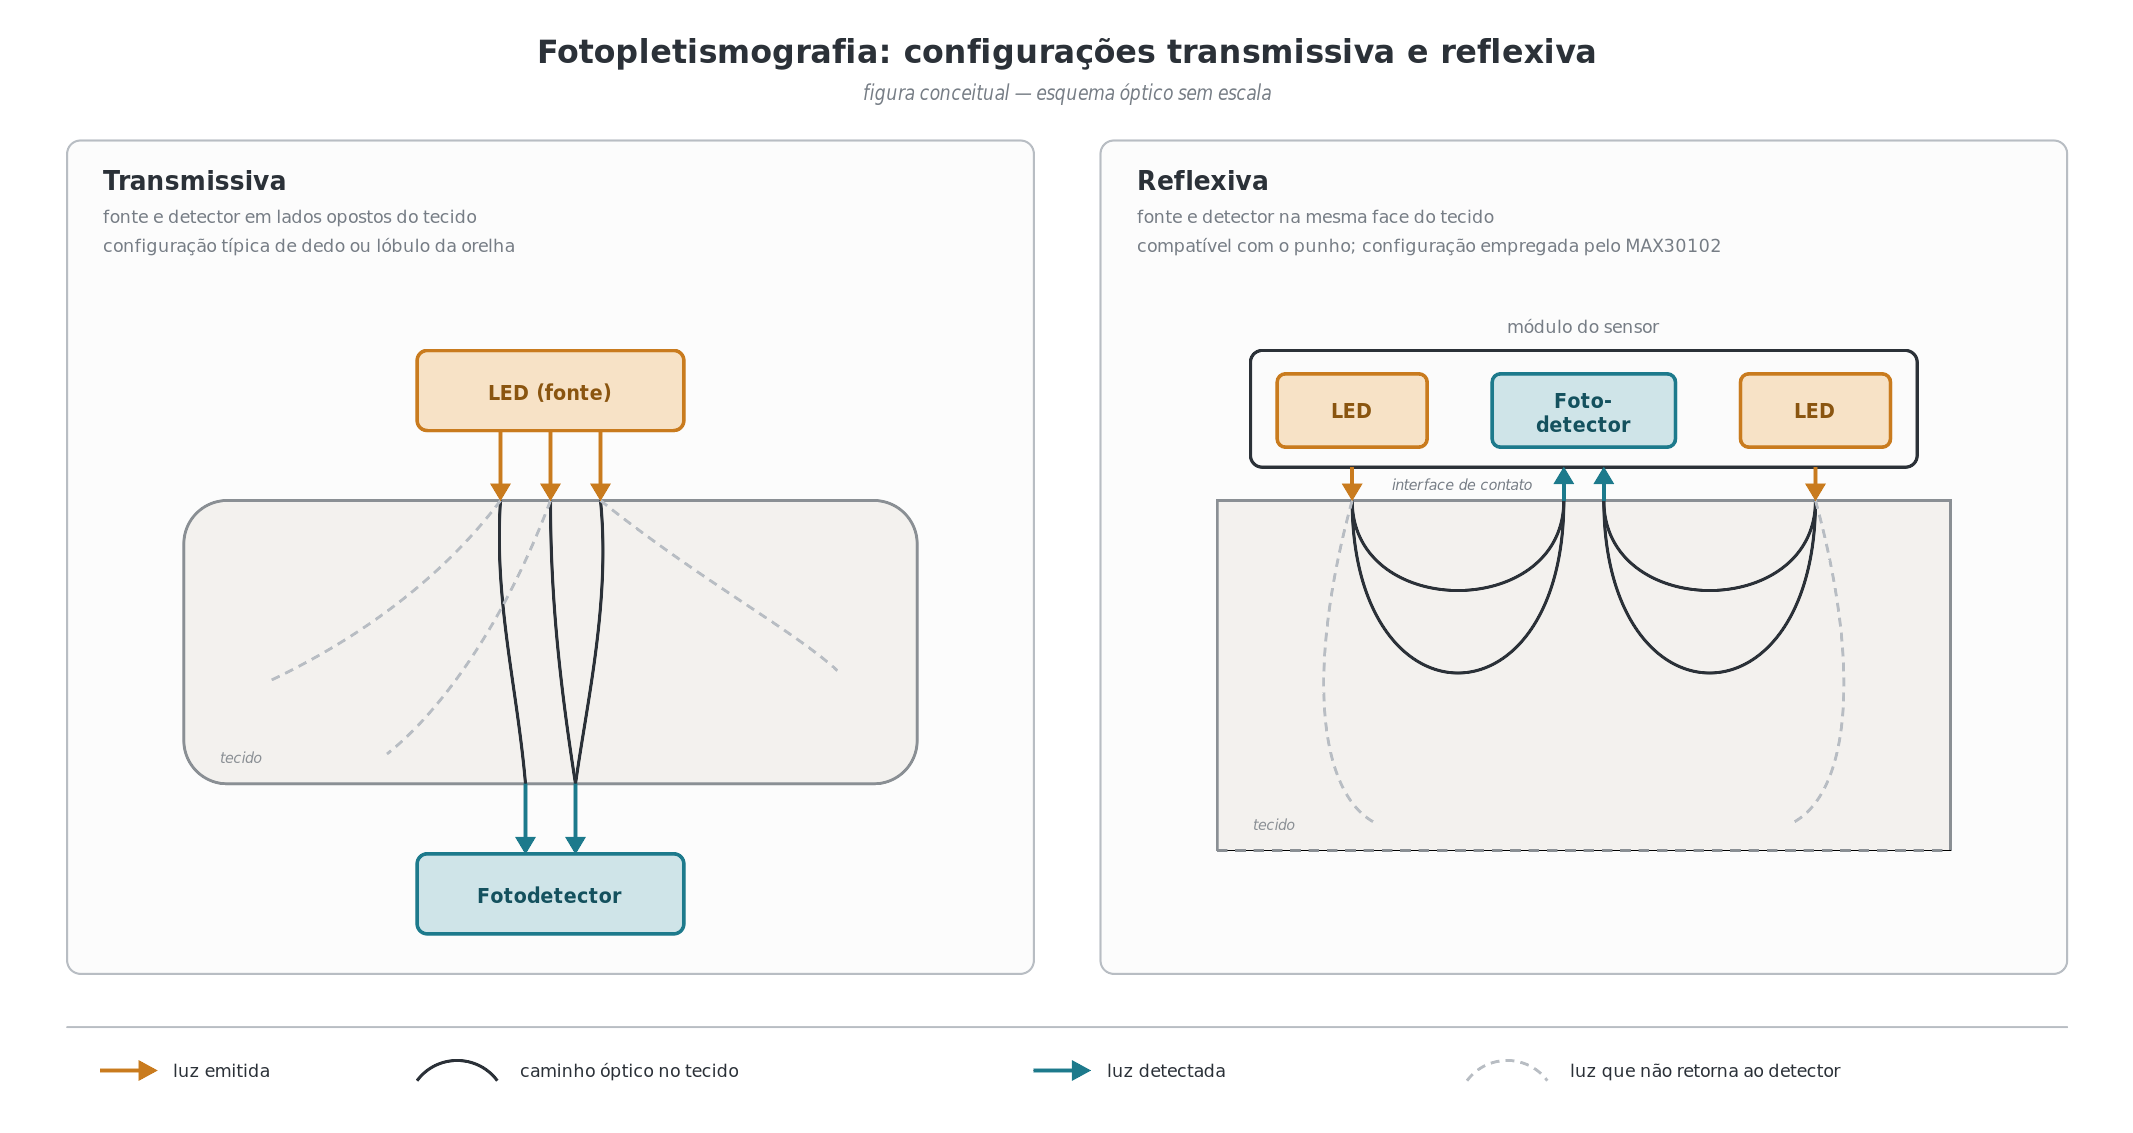
\includegraphics[width=0.94\textwidth]{ppg_transmissiva_reflexiva.png}
\fonteelemento{Elaborado pelo autor com base em Allen (2007), Tamura et al. (2014) e Analog Devices (2018)}
\end{figure}


\subsubsection{Componentes AC e DC}


O sinal PPG pode ser interpretado como a combina\c{c}\~ao de uma componente de varia\c{c}\~ao lenta, usualmente denominada DC, e uma componente puls\'atil, denominada AC. A componente DC re\'une a contribui\c{c}\~ao m\'edia dos tecidos, do sangue n\~ao puls\'atil, da geometria do contato e da intensidade \'optica recebida. A componente AC corresponde \`as varia\c{c}\~oes sincronizadas com a pulsa\c{c}\~ao arterial.


A amplitude AC \'e normalmente muito menor que o n\'ivel DC. O processamento precisa preservar a varia\c{c}\~ao puls\'atil sem saturar a cadeia de aquisi\c{c}\~ao e pode remover tend\^encias lentas para facilitar a detec\c{c}\~ao dos pulsos. Como altera\c{c}\~oes de contato ou movimento tamb\'em modificam o caminho \'optico, a separa\c{c}\~ao espectral n\~ao garante que toda varia\c{c}\~ao na faixa card\'iaca tenha origem fisiol\'ogica. A Figura~\ref{fig:ppg-ac-dc} apresenta essa decomposi\c{c}\~ao em valores normalizados e explicita a diferen\c{c}a de escala da componente puls\'atil.


\begin{figure}[H]
\centering
\caption{Decomposi\c{c}\~ao conceitual do sinal PPG em componentes DC e AC}
\label{fig:ppg-ac-dc}
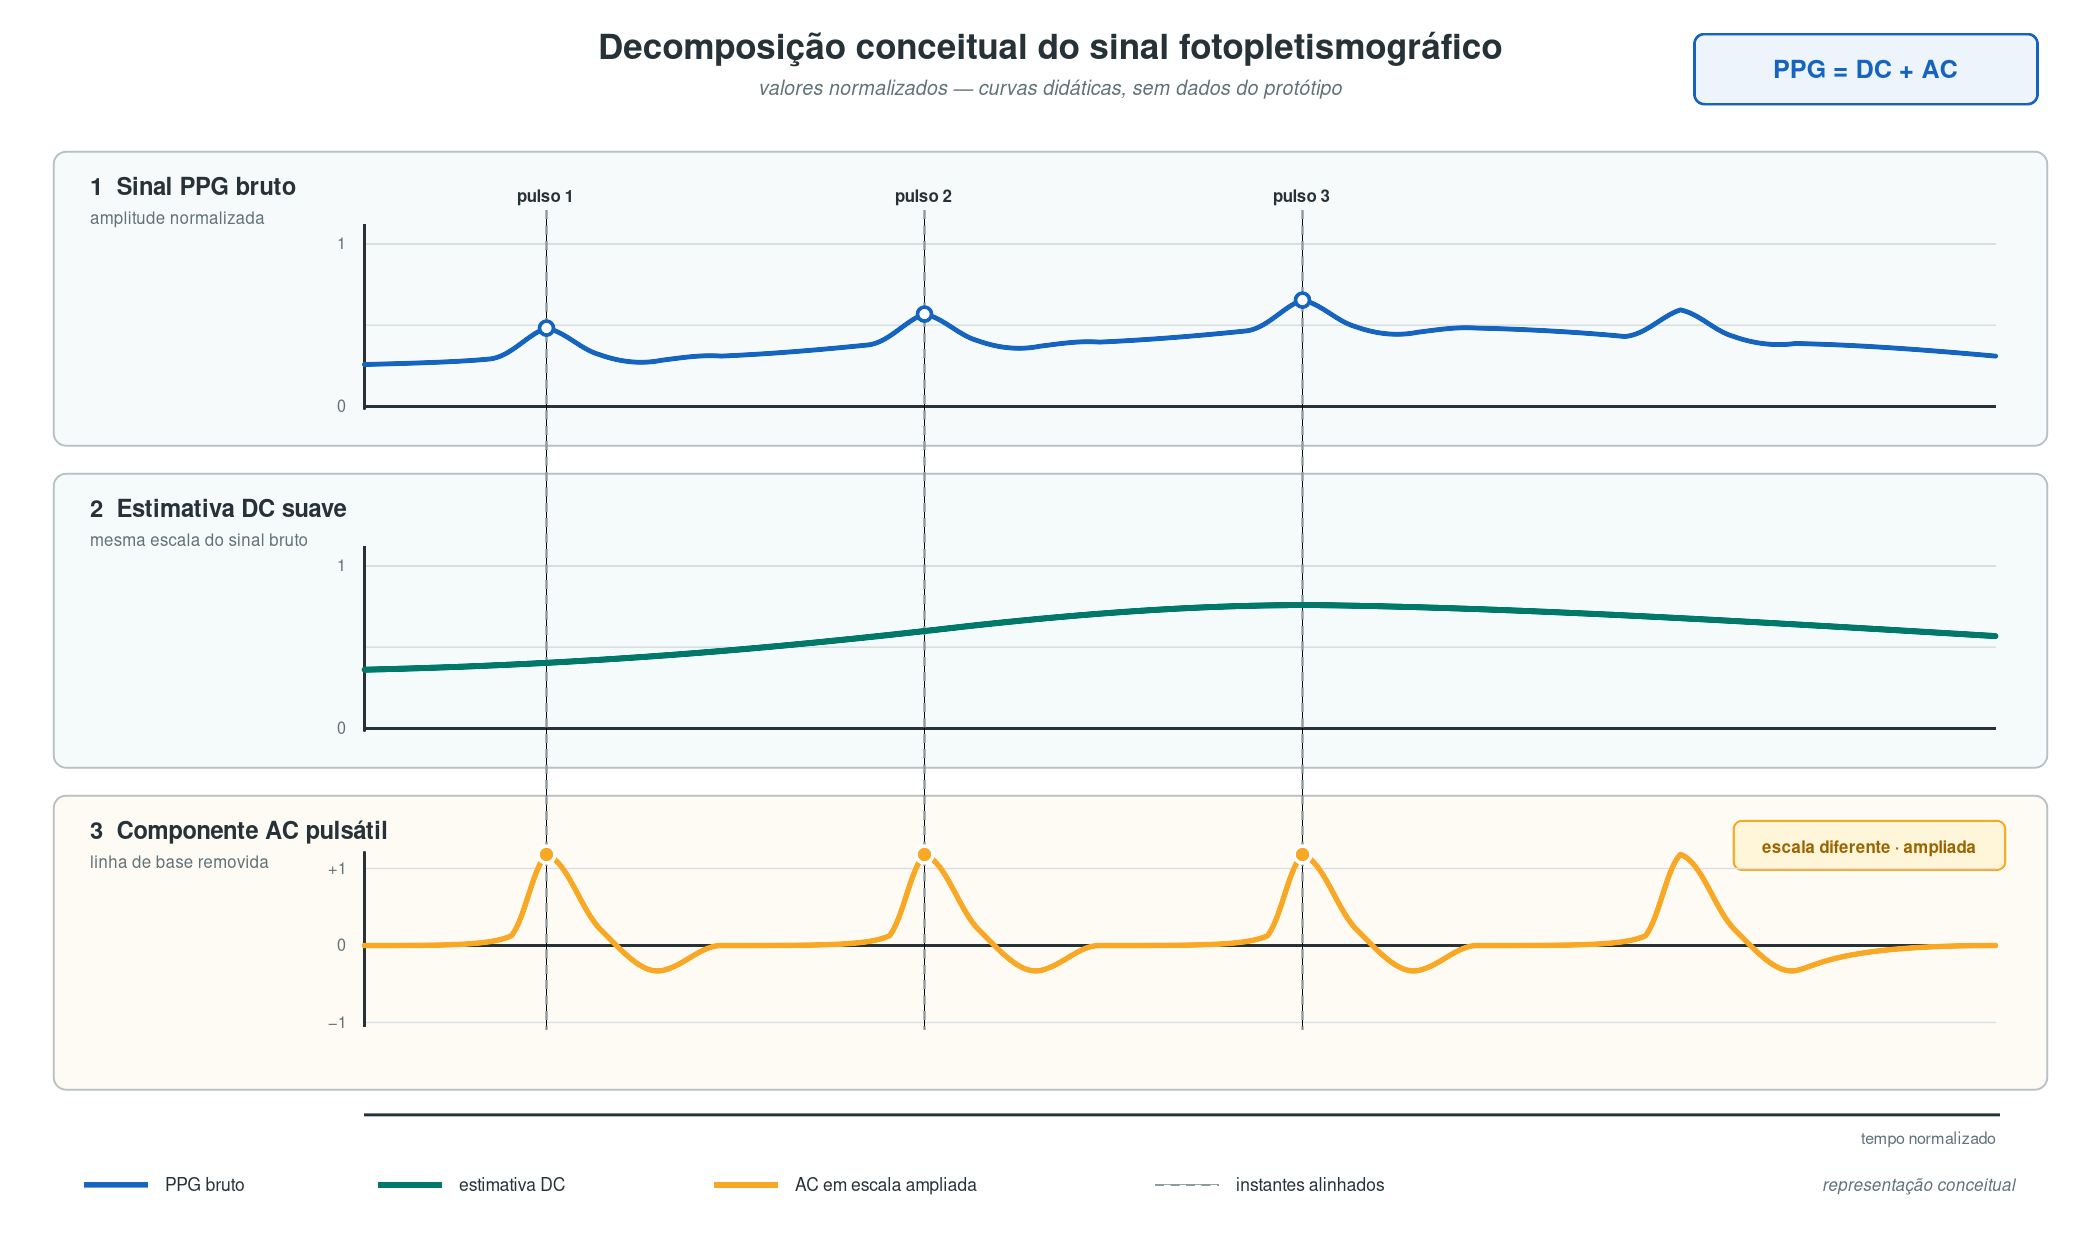
\includegraphics[width=0.94\textwidth]{ppg_componentes_ac_dc.png}
\fonteelemento{Elaborado pelo autor com base em Allen (2007)}
\end{figure}


\subsubsection{Frequ\^encia card\'iaca}


A frequ\^encia card\'iaca pode ser estimada a partir do intervalo entre pulsos consecutivos identificados no sinal PPG. Se \(T\) representa o intervalo m\'edio entre batimentos em segundos, a estimativa em batimentos por minuto \'e


\[
FC=\frac{60}{T}.
\]


O procedimento requer condicionamento do sinal e um crit\'erio para localizar pulsos v\'alidos. Filtragem, limiar, dist\^ancia m\'inima entre picos e rejei\c{c}\~ao de amplitudes incompat\'iveis podem reduzir detec\c{c}\~oes m\'ultiplas e ru\'ido. Esses par\^ametros precisam respeitar a faixa fisiol\'ogica de interesse e a frequ\^encia de amostragem; valores inadequados podem suprimir batimentos reais ou aceitar artefatos como pulsos.


Uma m\'edia calculada sobre v\'arios intervalos reduz a varia\c{c}\~ao da leitura, mas responde mais lentamente a mudan\c{c}as. A frequ\^encia card\'iaca produzida pelo algoritmo \'e uma estimativa dependente da qualidade do sinal e do m\'etodo de detec\c{c}\~ao, e n\~ao uma medi\c{c}\~ao direta da atividade el\'etrica do cora\c{c}\~ao.


\subsubsection{Estimativa de SpO$_2$}


A oximetria de pulso explora a diferen\c{c}a entre os espectros de absor\c{c}\~ao da hemoglobina oxigenada e desoxigenada. A aquisi\c{c}\~ao em dois comprimentos de onda permite comparar a modula\c{c}\~ao puls\'atil observada em cada canal. Uma formula\c{c}\~ao comum utiliza a raz\~ao de raz\~oes


\[
R=\frac{AC_{\mathrm{vermelho}}/DC_{\mathrm{vermelho}}}
        {AC_{\mathrm{infravermelho}}/DC_{\mathrm{infravermelho}}}.
\]


Uma rela\c{c}\~ao emp\'irica converte \(R\) em estimativa da satura\c{c}\~ao perif\'erica de oxig\^enio (SpO$_2$). Embora a lei de Beer--Lambert ajude a descrever a absor\c{c}\~ao em meios homog\^eneos, o tecido biol\'ogico apresenta espalhamento, m\'ultiplos constituintes e caminhos \'opticos vari\'aveis. Por isso, os coeficientes da convers\~ao n\~ao devem ser deduzidos apenas de um modelo ideal; dependem da geometria do sensor, do processamento e de calibra\c{c}\~ao contra valores de refer\^encia (ALLEN, 2007).


A apresenta\c{c}\~ao de uma estimativa de SpO$_2$ n\~ao caracteriza por si s\'o um ox\'imetro validado. O uso cl\'inico exige avalia\c{c}\~ao de exatid\~ao e desempenho segundo procedimentos e faixas apropriados. Sem essa valida\c{c}\~ao, o resultado deve permanecer identificado como estimativa experimental.


\subsubsection{Artefatos e limita\c{c}\~oes}


Movimento relativo entre sensor e pele altera a press\~ao de contato e o caminho percorrido pela luz. O artefato resultante pode ocupar a mesma faixa de frequ\^encias do sinal puls\'atil, o que limita sua remo\c{c}\~ao apenas por filtragem. Luz ambiente que alcan\c{c}a o fotodetector, contato insuficiente, satura\c{c}\~ao, baixa perfus\~ao e varia\c{c}\~oes de pigmenta\c{c}\~ao ou anatomia tamb\'em podem modificar a rela\c{c}\~ao sinal-ru\'ido (TAMURA et al., 2014).


No punho, gestos e marcha produzem componentes peri\'odicas que podem ser confundidas com batimentos. Sensores inerciais podem auxiliar a identificar per\'iodos de movimento, mas n\~ao garantem a reconstru\c{c}\~ao do sinal fisiol\'ogico. A avalia\c{c}\~ao deve incluir o sinal bruto, o sinal processado e condi\c{c}\~oes controladas de repouso e movimento, com registro de perdas de contato ou satura\c{c}\~ao.


As estimativas dependem ainda da taxa de amostragem, da estabilidade temporal, da corrente dos emissores, do ganho do receptor e dos filtros empregados. Compara\c{c}\~oes com um instrumento de refer\^encia precisam utilizar aquisi\c{c}\~ao temporalmente alinhada e popula\c{c}\~ao compat\'ivel com o uso pretendido.


\subsubsection{Aquisi\c{c}\~ao digital e compromissos de configura\c{c}\~ao}


Um sensor integrado como o MAX30102 combina emissores vermelho e infravermelho, fotodetector, eletr\^onica de condicionamento, conversor e fila de primeiro a entrar, primeiro a sair (First In, First Out --- FIFO), comunicando-se por I$^2$C (ANALOG DEVICES, 2018). A FIFO desacopla parcialmente o instante de amostragem do instante em que o processador atende o barramento, mas possui profundidade finita; se n\~ao for drenada a tempo, amostras podem ser sobrescritas ou perdidas conforme a configura\c{c}\~ao.


Taxa de amostragem, largura de pulso, faixa do conversor e corrente dos LEDs formam compromissos de resolu\c{c}\~ao, rela\c{c}\~ao sinal-ru\'ido, consumo e risco de satura\c{c}\~ao. Corrente \'optica maior n\~ao garante sinal utiliz\'avel se o receptor saturar, e faixa maior reduz a chance de satura\c{c}\~ao ao custo da resolu\c{c}\~ao relativa. A ordem dos canais definida pelo componente deve ser confirmada para a placa e o caminho de leitura empregados; uma invers\~ao observada em um m\'odulo espec\'ifico \'e evid\^encia de integra\c{c}\~ao, n\~ao propriedade universal do MAX30102.


\subsection{Sensoriamento de temperatura}


Sensores digitais de temperatura integram o elemento sens\'ivel, a convers\~ao e a interface de comunica\c{c}\~ao, fornecendo a medida em uma representa\c{c}\~ao num\'erica. Essa integra\c{c}\~ao reduz a necessidade de uma cadeia anal\'ogica externa, mas a exatid\~ao permanece condicionada \`as especifica\c{c}\~oes do sensor, \`a faixa de opera\c{c}\~ao, \`a montagem e ao equil\'ibrio t\'ermico com o meio observado.


Resolu\c{c}\~ao e exatid\~ao s\~ao caracter\'isticas distintas. A resolu\c{c}\~ao indica o menor incremento represent\'avel, enquanto a exatid\~ao expressa o limite de erro em rela\c{c}\~ao ao valor verdadeiro nas condi\c{c}\~oes especificadas. Uma leitura com mais casas bin\'arias n\~ao \'e necessariamente mais exata. Em sensores com resolu\c{c}\~ao configur\'avel, maior resolu\c{c}\~ao tamb\'em pode exigir maior tempo de convers\~ao.


Quando a temperatura \'e lida por contato, o encapsulamento, a condu\c{c}\~ao pelas conex\~oes, o fluxo de ar e fontes de calor pr\'oximas influenciam a resposta. Em um dispositivo vest\'ivel, uma medida na regi\~ao do punho n\~ao deve ser tratada automaticamente como temperatura corporal central. C\'odigos de verifica\c{c}\~ao, como a verifica\c{c}\~ao c\'iclica de redund\^ancia (Cyclic Redundancy Check --- CRC), detectam determinadas corrup\c{c}\~oes na comunica\c{c}\~ao, mas n\~ao corrigem erros t\'ermicos ou de posicionamento (ANALOG DEVICES, 2019).


O DS18B20 realiza convers\~ao digital configur\'avel de 9 a 12 bits e armazena o resultado em um \emph{scratchpad} protegido por CRC. O tempo m\'aximo de convers\~ao cresce com a resolu\c{c}\~ao selecionada, de modo que o controlador deve aguardar a conclus\~ao ou consult\'a-la antes de interpretar o resultado. Ap\'os energiza\c{c}\~ao, o registrador de temperatura apresenta 85~$^\circ$C at\'e que uma convers\~ao seja executada; esse valor deve ser interpretado com o estado da opera\c{c}\~ao, e n\~ao aceito isoladamente como temperatura do meio (ANALOG DEVICES, 2019).


O tempo necess\'ario para o encapsulamento aproximar-se da temperatura do objeto constitui resposta t\'ermica e \'e diferente do tempo de convers\~ao digital. Contato mec\^anico, massa t\'ermica, condu\c{c}\~ao pelos fios e convec\c{c}\~ao determinam uma constante de tempo efetiva da montagem. Filtrar ou aumentar a resolu\c{c}\~ao n\~ao acelera esse equil\'ibrio.


\subsection{Sensoriamento \'optico ambiental}


\subsubsection{Ilumin\^ancia}


Ilumin\^ancia \'e a grandeza fotom\'etrica que representa o fluxo luminoso incidente por unidade de \'area, ponderado pela sensibilidade espectral do sistema visual humano. Sua unidade no Sistema Internacional \'e o lux, equivalente a l\'umen por metro quadrado. Por utilizar pondera\c{c}\~ao fot\'opica, a ilumin\^ancia n\~ao corresponde simplesmente \`a pot\^encia \'optica total recebida pelo sensor.


Sensores de luz ambiente aproximam essa resposta por meio de sua sensibilidade espectral e de uma convers\~ao entre contagens digitais e lux. Ganho, tempo de integra\c{c}\~ao e faixa de medida afetam resolu\c{c}\~ao e satura\c{c}\~ao. A rela\c{c}\~ao de convers\~ao fornecida pelo fabricante pressup\~oe condi\c{c}\~oes definidas e pode ser alterada pela janela \'optica, pelo \^angulo de incid\^encia e pelo espectro da fonte (LITE-ON TECHNOLOGY, 2024).


\subsubsection{Radia\c{c}\~ao ultravioleta e UVI}


A radia\c{c}\~ao ultravioleta compreende comprimentos de onda menores que os da luz vis\'ivel. Para comunica\c{c}\~ao do risco da exposi\c{c}\~ao solar, o \'Indice Ultravioleta (Ultraviolet Index --- UVI) representa a irradi\^ancia ultravioleta ponderada pela a\c{c}\~ao eritematosa sobre a pele e escalonada por uma constante. Trata-se de uma grandeza adimensional, n\~ao de uma leitura direta em lux (WORLD HEALTH ORGANIZATION et al., 2002).


Um sensor com canal ultravioleta produz contagens relacionadas \`a radia\c{c}\~ao que alcan\c{c}a sua \'area sens\'ivel. A convers\~ao dessas contagens em UVI depende da resposta espectral, do ganho, do tempo de integra\c{c}\~ao, da calibra\c{c}\~ao e das condi\c{c}\~oes \'opticas de montagem. Barreiras transparentes no vis\'ivel podem atenuar significativamente o ultravioleta (LITE-ON TECHNOLOGY, 2024).


Uma estimativa local produzida por um sensor de baixo custo n\~ao \'e automaticamente equivalente ao UVI meteorol\'ogico. Instrumentos de refer\^encia aplicam resposta espectral e calibra\c{c}\~ao adequadas, enquanto o valor divulgado para uma regi\~ao tamb\'em pode envolver modelos e condi\c{c}\~oes atmosf\'ericas. A interpreta\c{c}\~ao deve conservar essa distin\c{c}\~ao.


\subsubsection{Modos, integra\c{c}\~ao e satura\c{c}\~ao}


O LTR390 compartilha a mesma cadeia de convers\~ao entre um modo de luz ambiente (Ambient Light Sensing --- ALS) e um modo de ultravioleta (Ultraviolet Sensing --- UVS); os dois canais n\~ao s\~ao adquiridos simultaneamente. A altern\^ancia requer configurar o modo e aguardar uma amostra correspondente \`a nova condi\c{c}\~ao. Uma leitura obtida durante a estabiliza\c{c}\~ao n\~ao deve ser misturada ao estado filtrado do outro canal (LITE-ON TECHNOLOGY, 2024).


O ganho multiplica a resposta antes da convers\~ao e favorece sinais pequenos, mas reduz a margem at\'e satura\c{c}\~ao. Maior tempo de integra\c{c}\~ao e resolu\c{c}\~ao podem melhorar a discrimina\c{c}\~ao de contagens, ao custo de menor taxa de atualiza\c{c}\~ao e maior probabilidade de saturar em incid\^encia intensa. Como ALS e UVS representam grandezas e respostas espectrais distintas, cada canal deve manter seus pr\'oprios par\^ametros de convers\~ao e estado de filtragem quando as leituras s\~ao alternadas.


\subsection{Sensoriamento inercial e magn\'etico}


\subsubsection{Aceler\^ometros MEMS}


Um aceler\^ometro baseado em sistemas microeletromec\^anicos (Microelectromechanical Systems --- MEMS) mede acelera\c{c}\~ao espec\'ifica ao longo de um ou mais eixos. Em repouso sobre uma superf\'icie, sua sa\'ida inclui a rea\c{c}\~ao associada ao campo gravitacional; em movimento, combina essa componente com acelera\c{c}\~oes produzidas pela din\^amica do dispositivo. Sensores triaxiais fornecem as componentes \(a_x\), \(a_y\) e \(a_z\) em um sistema de coordenadas fixado ao encapsulamento.


A magnitude


\[
\lVert\mathbf{a}\rVert=\sqrt{a_x^2+a_y^2+a_z^2}
\]


reduz a depend\^encia da orienta\c{c}\~ao dos eixos para detectar varia\c{c}\~oes de intensidade. Ela n\~ao elimina efeitos da posi\c{c}\~ao no corpo, rota\c{c}\~ao do dispositivo, impacto ou movimento do bra\c{c}o. Faixa de medi\c{c}\~ao, resolu\c{c}\~ao, frequ\^encia de amostragem e filtragem tamb\'em condicionam os eventos que podem ser distinguidos.


Desvios constantes, diferen\c{c}as de escala entre eixos, ru\'ido e desalinhamento introduzem erros. A calibra\c{c}\~ao pode estimar parte desses termos a partir de orienta\c{c}\~oes ou refer\^encias conhecidas, mas sua necessidade e seu procedimento dependem da aplica\c{c}\~ao.


Faixa de medi\c{c}\~ao e resolu\c{c}\~ao efetiva formam um compromisso: ampliar a faixa evita satura\c{c}\~ao em impactos, enquanto uma faixa menor atribui mais contagens por unidade de acelera\c{c}\~ao. A taxa de dados de sa\'ida (Output Data Rate --- ODR) limita as varia\c{c}\~oes temporais observ\'aveis e deve ser compat\'ivel com a filtragem aplicada. Filtragem insuficiente pode preservar ru\'ido e aliasing; filtragem excessiva pode atenuar eventos de passo.


O ADXL345 e o aceler\^ometro integrado ao MPU-9250 ilustram componentes capazes de fornecer acelera\c{c}\~ao triaxial, mas n\~ao s\~ao intercambi\'aveis sem considerar faixa, resolu\c{c}\~ao, ODR e interface. Um componente avaliado em prototipagem n\~ao deve ser apresentado como parte da plataforma final se foi substitu\'ido. No MPU-9250, um mesmo encapsulamento re\'une o girosc\'opio e o aceler\^ometro do n\'ucleo MPU-6500 com o magnet\^ometro AK8963 em outro \emph{die} (TDK INVENSENSE, 2016).


\subsubsection{Magnet\^ometros triaxiais}


Um magnet\^ometro triaxial mede as componentes do vetor densidade de fluxo magn\'etico segundo tr\^es eixos ortogonais. Em condi\c{c}\~oes ideais, a orienta\c{c}\~ao do sensor em rela\c{c}\~ao ao campo terrestre altera essas componentes sem alterar a magnitude do vetor. Na pr\'atica, a leitura inclui o campo de interesse, campos produzidos pelo pr\'oprio dispositivo, materiais pr\'oximos e erros do sensor.


O uso do magnet\^ometro como b\'ussola requer conhecer a correspond\^encia entre os eixos f\'isicos e o sistema de coordenadas adotado pelo software. Trocas de eixo e invers\~oes de sinal alteram o sentido angular calculado. A montagem e a orienta\c{c}\~ao gr\'afica precisam, portanto, empregar uma conven\c{c}\~ao comum.


No MPU-9250, o AK8963 pode ser acessado pelo controlador auxiliar interno ou exposto ao barramento principal por um modo de \emph{bypass}. Antes da medi\c{c}\~ao, coeficientes de ajuste de sensibilidade gravados em mem\'oria de fus\'iveis devem ser lidos segundo a sequ\^encia definida pelo fabricante e aplicados por eixo. Esse ajuste de f\'abrica converte a sensibilidade do componente, mas n\~ao substitui a calibra\c{c}\~ao das perturba\c{c}\~oes magn\'eticas introduzidas pela montagem e pelo ambiente (TDK INVENSENSE, 2016; AKM, 2013).


\subsubsection{Campo magn\'etico terrestre}


O campo magn\'etico terrestre pode ser representado por uma componente horizontal e uma componente vertical no local da medi\c{c}\~ao. A dire\c{c}\~ao da componente horizontal define o norte magn\'etico. Ela n\~ao coincide necessariamente com o norte geogr\'afico; o \^angulo entre ambos \'e denominado declina\c{c}\~ao magn\'etica e varia com posi\c{c}\~ao e tempo.


O campo medido no interior de um equipamento pode diferir do campo ambiente. Correntes el\'etricas, \'im\~as, alto-falantes, motores, parafusos e estruturas ferromagn\'eticas produzem perturba\c{c}\~oes. A proximidade de objetos externos tamb\'em pode tornar uma calibra\c{c}\~ao previamente obtida inadequada para aquele ambiente.


\subsubsection{Heading e calibra\c{c}\~ao}


O \emph{heading} \'e o \^angulo de orienta\c{c}\~ao no plano horizontal em rela\c{c}\~ao a uma dire\c{c}\~ao de refer\^encia. Quando o sensor permanece nivelado e os eixos \(x\) e \(y\) correspondem ao plano horizontal, ele pode ser calculado por uma fun\c{c}\~ao de arco tangente com dois argumentos, por exemplo


\[
\psi=\operatorname{atan2}(m_y,m_x).
\]


A ordem dos argumentos, os sinais e o deslocamento angular dependem da conven\c{c}\~ao dos eixos e do sentido positivo adotado. O resultado obtido do campo \'e referido ao norte magn\'etico; a convers\~ao para norte geogr\'afico exige aplicar a declina\c{c}\~ao local.


Perturba\c{c}\~oes aproximadamente constantes no sistema de coordenadas do sensor deslocam o centro da nuvem de medidas e s\~ao associadas ao efeito \emph{hard iron}. Materiais que deformam o campo podem alterar escalas e ortogonalidade, produzindo efeito \emph{soft iron}. Em tr\^es dimens\~oes, uma calibra\c{c}\~ao geral estima um vetor de deslocamento e uma transforma\c{c}\~ao matricial para aproximar a nuvem medida de uma esfera centrada na origem (RENAUDIN; AFZAL; LACHAPELLE, 2010).


Uma calibra\c{c}\~ao baseada somente nos extremos de cada eixo corrige deslocamentos e escalas diagonais, mas n\~ao representa acoplamentos entre eixos. Al\'em disso, o c\'alculo bidimensional sem compensa\c{c}\~ao de inclina\c{c}\~ao pressup\~oe que o sensor permane\c{c}a aproximadamente nivelado. Quando essa condi\c{c}\~ao n\~ao \'e satisfeita, a componente vertical do campo \'e projetada nos eixos usados no c\'alculo e introduz erro angular. A Figura~\ref{fig:calibracao-magnetica} compara as nuvens ideal, deslocada, deformada e corrigida, destacando o alcance limitado da corre\c{c}\~ao diagonal.


\begin{figure}[H]
\centering
\caption{Efeitos de \emph{hard iron} e \emph{soft iron} e alcance da corre\c{c}\~ao diagonal}
\label{fig:calibracao-magnetica}
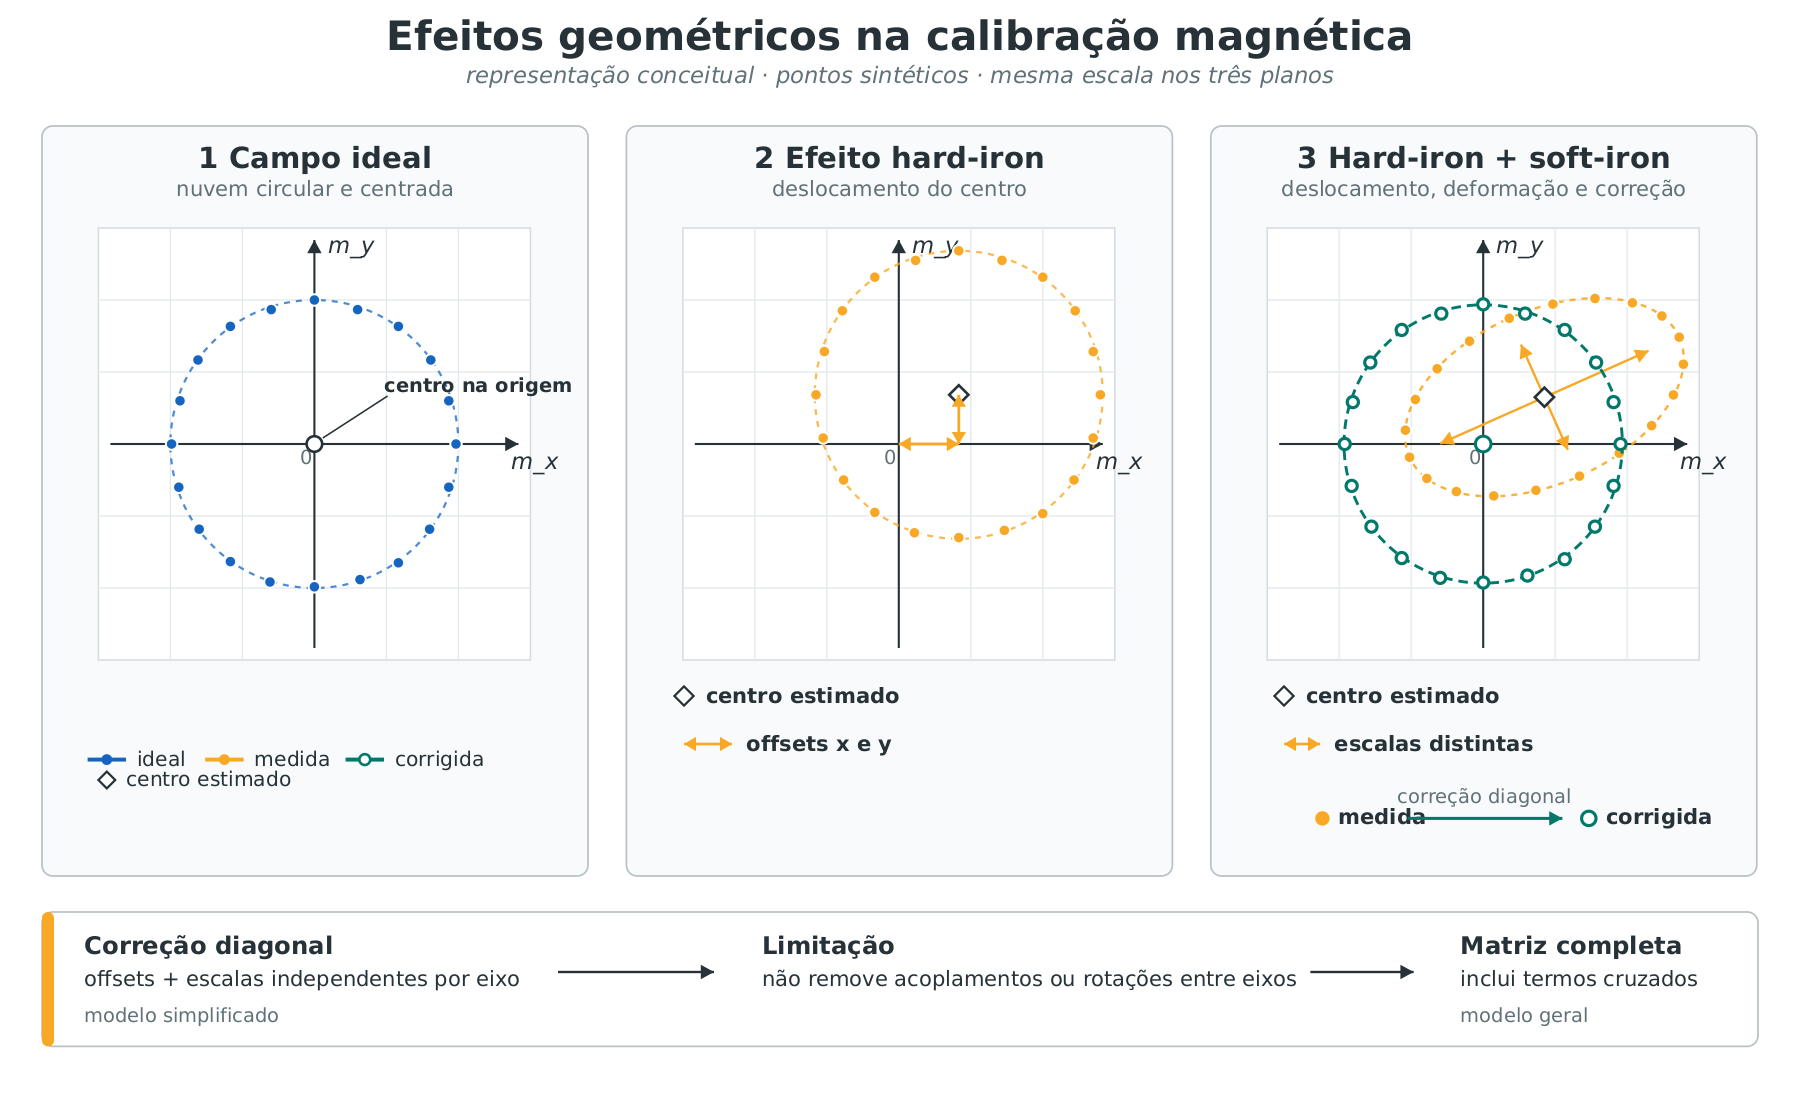
\includegraphics[width=0.94\textwidth]{calibracao_magnetica.png}
\fonteelemento{Elaborado pelo autor com base em Renaudin, Afzal e Lachapelle (2010)}
\end{figure}


A compensa\c{c}\~ao de inclina\c{c}\~ao usa uma estimativa de atitude, normalmente obtida do aceler\^ometro e eventualmente do girosc\'opio, para projetar o vetor magn\'etico no plano horizontal antes do c\'alculo angular. Ela reduz o erro geom\'etrico associado \`a inclina\c{c}\~ao, mas introduz depend\^encia da calibra\c{c}\~ao e da din\^amica dos sensores inerciais. No escopo deste trabalho, esse recurso \'e fundamento para uma extens\~ao futura: o algoritmo final avaliado calcula \emph{heading} bidimensional e pressup\~oe o dispositivo aproximadamente nivelado.


\subsubsection{Marcha e pedometria}


A marcha produz padr\~oes recorrentes de acelera\c{c}\~ao associados \`as fases do passo. Um ped\^ometro procura identificar esses eventos em meio a movimentos que n\~ao correspondem \`a caminhada. M\'etodos simples aplicam filtragem, limiares e busca de picos \`a magnitude da acelera\c{c}\~ao ou a um eixo selecionado.


Um limiar de amplitude rejeita varia\c{c}\~oes pequenas, enquanto um intervalo m\'inimo entre detec\c{c}\~oes evita contar v\'arias oscila\c{c}\~oes do mesmo passo. Limiares fixos podem falhar quando a intensidade da marcha, o usu\'ario ou a posi\c{c}\~ao do dispositivo mudam. Estrat\'egias adaptativas e o uso de caracter\'isticas temporais podem ampliar a faixa de funcionamento, com maior custo e necessidade de parametriza\c{c}\~ao (BRAJDIC; HARLE, 2013).


Uma m\'edia m\'ovel exponencial (Exponential Moving Average --- EMA) de primeira ordem atualiza o estado filtrado por


\[
y_k=\alpha x_k+(1-\alpha)y_{k-1}, \qquad 0<\alpha\leq 1,
\]


em que \(x_k\) \'e a amostra corrente. Valores menores de \(\alpha\) suavizam mais o sinal e aumentam o atraso. Em uma detec\c{c}\~ao por limiar, a histerese usa limites diferentes para armar e confirmar o evento, reduzindo comuta\c{c}\~oes repetidas pr\'oximas ao limiar. Um per\'iodo refrat\'ario rejeita novos eventos por um intervalo ap\'os um passo aceito; ele reduz contagens m\'ultiplas, mas pode suprimir passos reais se for incompat\'ivel com a cad\^encia. A Figura~\ref{fig:pedometro-limiar} relaciona o sinal filtrado, o limiar e o intervalo refrat\'ario na aceita\c{c}\~ao ou rejei\c{c}\~ao de picos.


Movimentos r\'itmicos do bra\c{c}o, transporte do dispositivo fora do punho e vibra\c{c}\~oes podem gerar falsos positivos; passos suaves podem resultar em falsos negativos. A valida\c{c}\~ao exige trajetos ou sequ\^encias controladas, contagem de refer\^encia e condi\c{c}\~oes declaradas de uso. A compara\c{c}\~ao entre passos detectados e passos reais pode ser expressa por erro absoluto, erro relativo e distribui\c{c}\~ao dos erros entre repeti\c{c}\~oes.


\begin{figure}[H]
\centering
\caption{Detec\c{c}\~ao conceitual de passos por limiar e intervalo refrat\'ario}
\label{fig:pedometro-limiar}
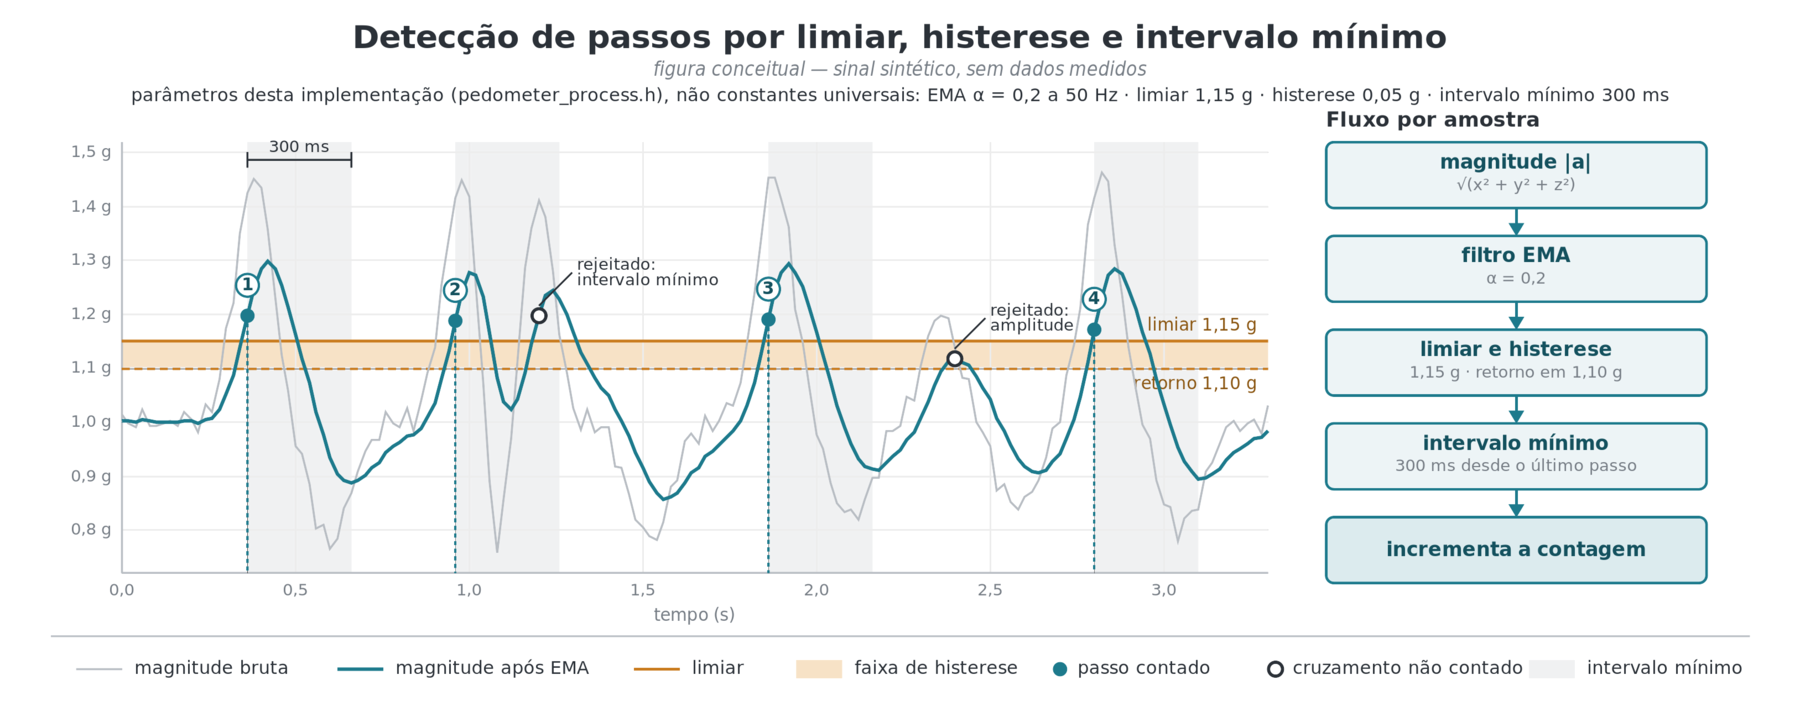
\includegraphics[width=0.94\textwidth]{pedometro_limiar.png}
\fonteelemento{Elaborado pelo autor com base em Brajdic e Harle (2013)}
\end{figure}


\subsection{Trabalhos relacionados}


\subsubsection{Crit\'erios de compara\c{c}\~ao}


Os trabalhos relacionados foram selecionados por apresentarem plataformas vest\'iveis program\'aveis, aquisi\c{c}\~ao multissensor ou organiza\c{c}\~ao destinada a m\'ultiplas aplica\c{c}\~oes. A compara\c{c}\~ao considera plataforma, sistema operacional, sensores, modularidade, extensibilidade, toler\^ancia a falhas, forma de avalia\c{c}\~ao e disponibilidade de c\'odigo. Os termos n\~ao s\~ao tratados como equivalentes quando descrevem n\'iveis distintos: modularidade f\'isica de sensores, modularidade de software e suporte a m\'ultiplas aplica\c{c}\~oes s\~ao registrados separadamente.


\subsubsection{Plataformas vest\'iveis abertas e multissensores}


Hester et al. (2016) apresentam o Amulet, uma plataforma vest\'ivel de baixo consumo destinada \`a execu\c{c}\~ao simult\^anea de aplica\c{c}\~oes. O sistema combina hardware pr\'oprio, sistema operacional e cadeia de ferramentas, com isolamento de mem\'oria e controle de acesso a recursos. A avalia\c{c}\~ao enfatiza consumo de energia e execu\c{c}\~ao de m\'ultiplas aplica\c{c}\~oes. Inclus\~ao de sensores por um contrato uniforme de m\'odulos e continuidade diante da aus\^encia de perif\'ericos n\~ao s\~ao as unidades de an\'alise adotadas nesse estudo.


Baldini et al. (2023) prop\~oem uma plataforma vest\'ivel aberta para aquisi\c{c}\~ao e processamento em tempo real de sinais fisiol\'ogicos. A organiza\c{c}\~ao distribui aquisi\c{c}\~ao, fus\~ao e armazenamento remoto entre blocos conectados e permite integrar diferentes dispositivos de medi\c{c}\~ao. O foco da avalia\c{c}\~ao est\'a na aquisi\c{c}\~ao sincronizada e no monitoramento remoto, em uma arquitetura de sistema mais ampla que o firmware de um \'unico smartwatch.


Van Dijk, Gawehns e Van Leeuwen (2023) apresentam o WEARDA, software aberto para registrar dados brutos de aceler\^ometro, girosc\'opio, bar\^ometro e sistema de posicionamento em um smartwatch comercial. O trabalho privilegia transpar\^encia, reprodutibilidade da coleta e apoio a estudos de atividade humana. Extensibilidade da arquitetura embarcada e recupera\c{c}\~ao de falhas de barramento ficam fora da unidade de an\'alise, pois o software utiliza sensores e interfaces oferecidos pelo sistema operacional do dispositivo. O Quadro~\ref{qua:trabalhos-relacionados} sintetiza as diferentes unidades de an\'alise e formas de avalia\c{c}\~ao desses trabalhos.


\begin{quadro}[ht]
\centering
\caption{Compara\c{c}\~ao entre plataformas vest\'iveis relacionadas}
\label{qua:trabalhos-relacionados}
\small
\renewcommand{\arraystretch}{1.15}
\begin{tabularx}{\textwidth}{>{\raggedright\arraybackslash}p{0.17\textwidth}*{3}{>{\raggedright\arraybackslash}X}}
\toprule
\textbf{Trabalho} & \textbf{\^Enfase} & \textbf{Organiza\c{c}\~ao e extens\~ao} & \textbf{Avalia\c{c}\~ao reportada} \\
\midrule
Amulet (HESTER et al., 2016) & Plataforma vest\'ivel para m\'ultiplas aplica\c{c}\~oes & Sistema operacional, isolamento e acesso controlado a recursos & Energia e execu\c{c}\~ao de aplica\c{c}\~oes \\
\addlinespace
WMP (BALDINI et al., 2023) & Aquisi\c{c}\~ao fisiol\'ogica multissensor em tempo real & Blocos de aquisi\c{c}\~ao, fus\~ao e processamento remoto & Aquisi\c{c}\~ao sincronizada e aplica\c{c}\~ao de monitoramento \\
\addlinespace
WEARDA (VAN DIJK; GAWEHNS; VAN LEEUWEN, 2023) & Coleta aberta de dados brutos em smartwatch comercial & Fun\c{c}\~oes de registro sobre sensores expostos pelo Tizen & Uso em coleta de atividade e reprodutibilidade \\
\bottomrule
\end{tabularx}
\fonteelemento{Elaborado pelo autor com base em Hester et al. (2016), Baldini et al. (2023) e Van Dijk, Gawehns e Van Leeuwen (2023)}
\end{quadro}


Os tr\^es trabalhos demonstram que plataformas vest\'iveis podem ser estudadas al\'em de uma aplica\c{c}\~ao isolada, por\'em adotam unidades de an\'alise diferentes. O Amulet concentra-se na coexist\^encia de aplica\c{c}\~oes e no consumo; a WMP, na aquisi\c{c}\~ao fisiol\'ogica conectada; e o WEARDA, na coleta reprodut\'ivel com hardware comercial. Nenhum deles apresenta conjuntamente, como objeto de avalia\c{c}\~ao, um contrato uniforme para m\'odulos de sensores heterog\^eneos, coordena\c{c}\~ao expl\'icita de um barramento compartilhado, inicializa\c{c}\~ao n\~ao fatal e ensaios de opera\c{c}\~ao com sensores ausentes. Essa delimita\c{c}\~ao estabelece os crit\'erios de compara\c{c}\~ao do presente trabalho sem pressupor que propriedades n\~ao medidas estejam ausentes das plataformas relacionadas.

\clearpage
\section{Materiais e M\'etodos}


Este cap\'itulo descreve os recursos empregados na constru\c{c}\~ao do prot\'otipo, o m\'etodo adotado para desenvolver a plataforma e os procedimentos definidos para sua avalia\c{c}\~ao. A descri\c{c}\~ao da implementa\c{c}\~ao interna dos servi\c{c}os, drivers e m\'odulos \'e apresentada no cap\'itulo de Desenvolvimento, enquanto os valores medidos e sua interpreta\c{c}\~ao pertencem ao cap\'itulo de Resultados e Discuss\~ao.


Os procedimentos de ensaio foram formulados para permitir repeti\c{c}\~ao sob condi\c{c}\~oes declaradas. O firmware integrado, o caderno de ensaios, os arquivos de dados, os scripts de tratamento e as imagens correspondentes foram usados para distinguir procedimentos executados de pilotos, observa\c{c}\~oes qualitativas e atividades retiradas do escopo temporal desta vers\~ao. Nenhum resultado \'e antecipado neste cap\'itulo.


\subsection{Materiais}


\subsubsection{Unidade de processamento}


A unidade de processamento utilizada foi a placa Seeed Studio XIAO ESP32-C6, baseada no sistema em chip ESP32-C6. O processador principal emprega arquitetura RISC-V de 32 bits e opera a at\'e 160 MHz. O dispositivo disp\~oe de 512 KiB de SRAM de alto desempenho e a placa cont\'em 4 MiB de mem\'oria \emph{flash}. Seu formato de 21 $\times$ 17,8 mm permite o encaixe na placa de expans\~ao circular utilizada no prot\'otipo (SEEED STUDIO, 2024).


A escolha considerou a compatibilidade mec\^anica com o Round Display, a disponibilidade de controladores para I$^2$C, SPI, RMT e GPIO, os recursos necess\'arios \`a interface gr\'afica e o suporte oficial do ESP-IDF. As interfaces sem fio presentes no ESP32-C6 n\~ao constitu\'iram requisito da vers\~ao avaliada e n\~ao foram utilizadas como justificativa de resultados de conectividade ou consumo.


\subsubsection{Round Display}


A interface f\'isica foi constru\'ida sobre o Seeed Studio Round Display for XIAO, uma placa circular de 39 mm com display sens\'ivel ao toque de 1,28 polegada, resolu\c{c}\~ao de 240 $\times$ 240 pixels e profundidade de 16 bits. A placa tamb\'em cont\'em circuito de carregamento para bateria, conector para bateria, slot para cart\~ao microSD e um RTC PCF8563 (SEEED STUDIO, [s.d.]).


O painel \'e controlado pelo GC9A01A e recebe comandos e pixels RGB565 pelo perif\'erico SPI2. No prot\'otipo, a interface opera a 40 MHz e utiliza somente transmiss\~ao para o display. O toque capacitivo do exemplar utilizado \'e controlado pelo CHSC6X, identificado no endere\c{c}o I$^2$C 0x2E. Essa identifica\c{c}\~ao decorre do hardware efetivamente recebido e difere do controlador indicado em parte da documenta\c{c}\~ao hist\'orica da placa.


O PCF8563, no endere\c{c}o I$^2$C 0x51, mant\'em segundos, minutos, horas e calend\'ario. A bateria de reserva instalada no Round Display permite conservar essas informa\c{c}\~oes quando a alimenta\c{c}\~ao principal \'e removida. O backlight permaneceu ligado durante a opera\c{c}\~ao porque seu controle por software n\~ao ficou dispon\'ivel na combina\c{c}\~ao de revis\~ao de placa e XIAO ESP32-C6 utilizada.


\subsubsection{Sensores}


\paragraph{MAX30102}


O MAX30102 \'e um sensor \'optico reflexivo que integra emissores vermelho e infravermelho, fotodetector, conversor de 18 bits, rejei\c{c}\~ao de luz ambiente e FIFO com 32 posi\c{c}\~oes. O componente comunica-se por I$^2$C no endere\c{c}o 0x57 e permite configurar corrente dos emissores, largura dos pulsos, taxa de amostragem e faixa do conversor (ANALOG DEVICES, 2018).


No prot\'otipo, o sensor foi empregado para adquirir os canais de PPG utilizados na estimativa de frequ\^encia card\'iaca e de SpO$_2$. A placa de conex\~ao utilizada integra a alimenta\c{c}\~ao exigida pelo componente. Como os resultados n\~ao possuem valida\c{c}\~ao cl\'inica, o m\'odulo foi tratado como demonstrador de aquisi\c{c}\~ao e processamento de sinais fisiol\'ogicos.


\paragraph{DS18B20}


O DS18B20 \'e um sensor digital de temperatura com interface 1-Wire, resolu\c{c}\~ao configur\'avel entre 9 e 12 bits e verifica\c{c}\~ao CRC dos dados. Foi utilizado com alimenta\c{c}\~ao externa de 3,3 V, resolu\c{c}\~ao de 11 bits e resistor de \emph{pull-up} de 4,7 k$\Omega$ entre a linha de dados e a alimenta\c{c}\~ao. A comunica\c{c}\~ao foi realizada no GPIO20 por meio do perif\'erico RMT e dos componentes oficiais \texttt{onewire\_bus} e \texttt{ds18b20} (ANALOG DEVICES, 2019).


O sensor foi destinado \`a observa\c{c}\~ao de temperatura ambiente. Sua posi\c{c}\~ao na montagem provis\'oria, a aus\^encia de encapsulamento final e a influ\^encia t\'ermica do pr\'oprio prot\'otipo devem ser registradas em cada ensaio, pois uma leitura no dispositivo n\~ao representa automaticamente a temperatura corporal.


\paragraph{LTR390}


O LTR390 integra um canal para luz ambiente e outro para radia\c{c}\~ao ultravioleta, selecionados de forma alternada, e fornece os resultados por I$^2$C no endere\c{c}o 0x53. Ganho e tempo de integra\c{c}\~ao configur\'aveis determinam a resolu\c{c}\~ao e o limite de satura\c{c}\~ao. A convers\~ao das contagens depende da configura\c{c}\~ao aplicada e das rela\c{c}\~oes fornecidas pelo fabricante (LITE-ON TECHNOLOGY, 2024).


O mesmo componente foi empregado para estimar ilumin\^ancia e UVI. Como os canais n\~ao s\~ao convertidos simultaneamente, o m\'etodo de opera\c{c}\~ao alterna o modo conforme a fun\c{c}\~ao ativa e descarta as primeiras amostras ap\'os a mudan\c{c}a para permitir a estabiliza\c{c}\~ao. A estimativa de UVI do prot\'otipo n\~ao foi equiparada a uma medi\c{c}\~ao meteorol\'ogica de refer\^encia.


\paragraph{MPU-9250 e AK8963}


O m\'odulo inercial empregado foi baseado no MPU-9250, que re\'une aceler\^ometro e girosc\'opio triaxiais e permite acesso ao magnet\^ometro AK8963. O MPU-9250 foi ligado ao barramento I$^2$C no endere\c{c}o 0x68; o AK8963 foi acessado no endere\c{c}o 0x0C por meio do modo \emph{bypass} do MPU-9250 (TDK INVENSENSE, 2016).


As acelera\c{c}\~oes foram utilizadas pelo ped\^ometro implementado em software. As medidas magn\'eticas foram utilizadas para a b\'ussola ap\'os corre\c{c}\~ao de deslocamento e escala obtida por calibra\c{c}\~ao executada no pr\'oprio dispositivo. Os par\^ametros de calibra\c{c}\~ao foram armazenados em mem\'oria n\~ao vol\'atil. O c\'alculo de \emph{heading} n\~ao inclui compensa\c{c}\~ao de inclina\c{c}\~ao e pressup\~oe que o dispositivo esteja aproximadamente nivelado.


\subsubsection{Instrumentos de bancada}

Foram empregados um mult\'imetro digital para medir tens\~ao e corrente, um ox\'imetro de dedo ECH de modelo n\~ao identificado para compara\c{c}\~ao funcional de frequ\^encia card\'iaca e SpO$_2$, um termo-higr\^ometro MFL modelo Embutir para compara\c{c}\~ao de temperatura e uma b\'ussola magn\'etica Norvix DC45-2 para compara\c{c}\~ao de \emph{heading}. Um Amazfit Active 2 foi usado como corrobora\c{c}\~ao no ensaio de PPG e como comparador secund\'ario no ensaio do ped\^ometro. Uma lanterna comum e uma lanterna UV gen\'erica foram utilizadas somente como est\'imulos funcionais dos canais de ilumin\^ancia e ultravioleta do LTR390.

Os instrumentos de consumo n\~ao possu\'iam certificado de calibra\c{c}\~ao dispon\'ivel. Consequentemente, as compara\c{c}\~oes foram classificadas como testes funcionais ou verifica\c{c}\~oes de plausibilidade, e n\~ao como valida\c{c}\~oes metrol\'ogicas ou cl\'inicas. As fotografias do ox\'imetro e do termo-higr\^ometro correspondem aos aparelhos efetivamente empregados.


\subsubsection{Ferramentas de software}


O firmware foi desenvolvido em C com ESP-IDF 5.5.1. O FreeRTOS fornecido pelo ambiente foi utilizado em configura\c{c}\~ao de n\'ucleo \'unico, e a interface gr\'afica foi constru\'ida com LVGL v8. O SquareLine Studio 1.6.0 foi empregado somente na cria\c{c}\~ao da base visual da tela principal, aproximando-a do desenho pretendido. Como os recursos gr\'aficos exportados ocupavam parcela relevante da mem\'oria flash, as demais telas foram implementadas diretamente com a API do LVGL. A compila\c{c}\~ao e a an\'alise do tamanho da aplica\c{c}\~ao utilizaram as ferramentas do ESP-IDF. O monitor serial e os n\'iveis de log foram empregados no diagn\'ostico de inicializa\c{c}\~ao, comunica\c{c}\~ao e tarefas.


Foram usados os componentes LVGL 8.4.0, \texttt{esp\_lcd\_gc9a01} 2.0.4, \texttt{esp\_lcd\_touch} 1.2.1, \texttt{esp\_lvgl\_port} 2.8.0-1, \texttt{onewire\_bus} 1.1.1 e \texttt{ds18b20} 0.1.2, conforme o arquivo \texttt{dependencies.lock}. Drivers pr\'oprios foram adotados para MAX30102, LTR390, MPU-9250/AK8963, PCF8563 e CHSC6X.


\subsubsection{Montagem e mapa de liga\c{c}\~oes}


A integra\c{c}\~ao f\'isica foi realizada em uma placa prot\'otipo autoral, acompanhada de inv\'olucro fabricado por impress\~ao 3D. O XIAO ESP32-C6 permaneceu encaixado no Round Display, e os sensores externos foram distribu\'idos na placa conforme o esquema e o leiaute documentados. O barramento I$^2$C foi compartilhado pelos sensores, pelo toque e pelo RTC, operando a 100 kHz em SDA GPIO22 e SCL GPIO23. A Figura~\ref{fig:placa-prototipo} registra a placa em funcionamento, enquanto a Figura~\ref{fig:pcb-render} apresenta as duas faces previstas no projeto.


\begin{figure}[H]
\centering
\caption{Placa prot\'otipo com display e m\'odulos durante a opera\c{c}\~ao}
\label{fig:placa-prototipo}
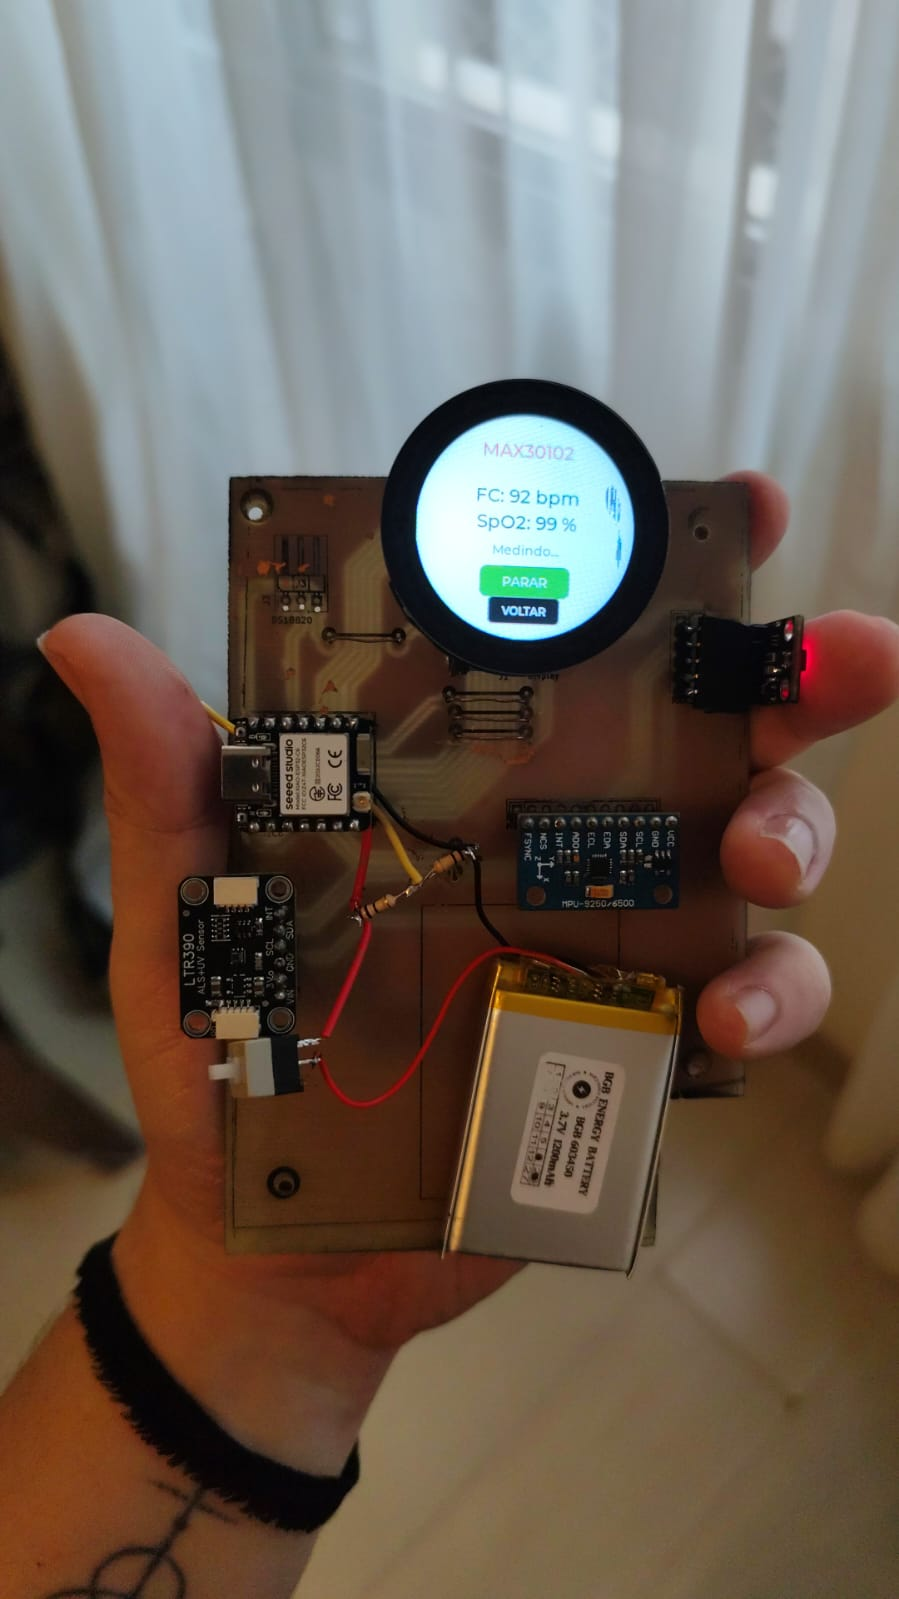
\includegraphics[width=0.48\textwidth]{PCB/Prototipo.jpeg}
\begin{minipage}{0.48\textwidth}
\fonteelemento{Acervo do autor}
\end{minipage}
\end{figure}


\begin{figure}[H]
\centering
\caption{Renderiza\c{c}\~oes das faces da placa desenvolvida}
\label{fig:pcb-render}
\begin{subfigure}[t]{0.44\textwidth}
\centering
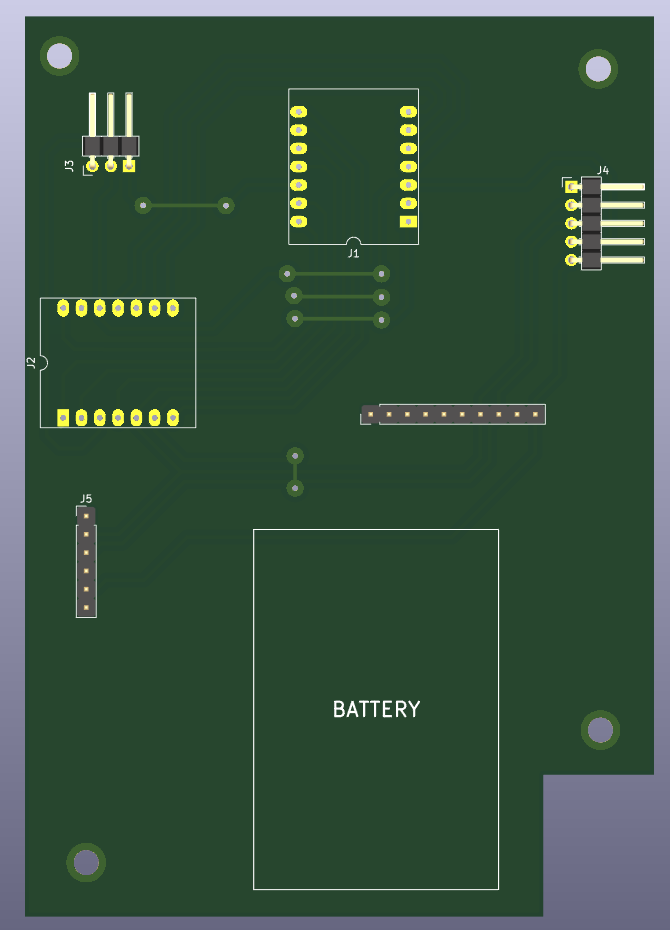
\includegraphics[width=\linewidth]{PCB/3dtoplayer.png}
\caption{Face superior}
\end{subfigure}
\hfill
\begin{subfigure}[t]{0.44\textwidth}
\centering
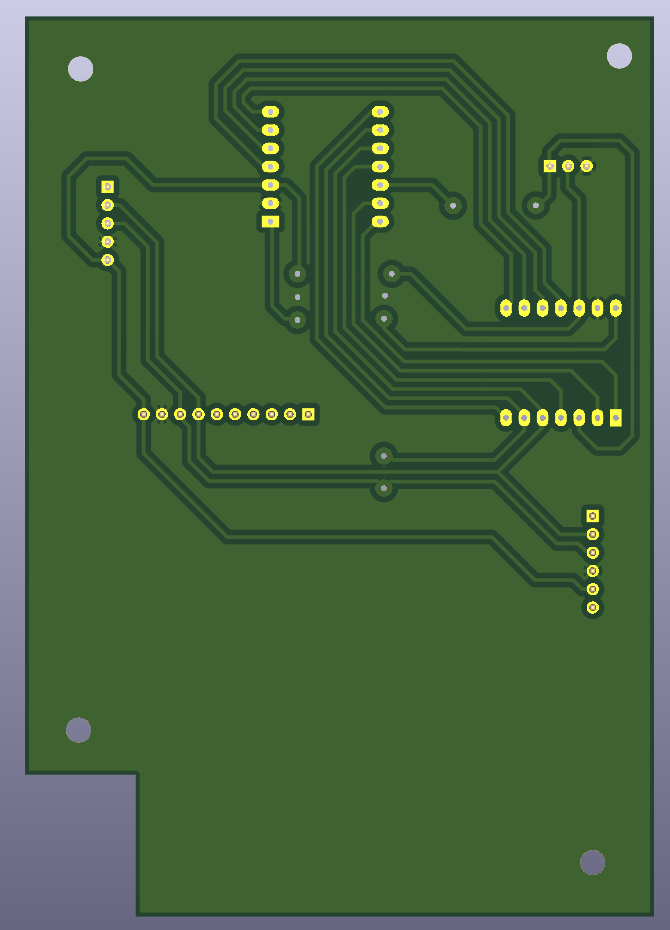
\includegraphics[width=\linewidth]{PCB/3dbottomlayer.png}
\caption{Face inferior}
\end{subfigure}
\begin{minipage}{0.92\textwidth}
\fonteelemento{Elaborado pelo autor a partir do projeto da placa}
\end{minipage}
\end{figure}


O Quadro~\ref{qua:mapa-interfaces} consolida as interfaces e conex\~oes confirmadas no firmware integrado.


\begin{quadro}[H]
\centering
\caption{Mapa consolidado de interfaces e liga\c{c}\~oes}
\label{qua:mapa-interfaces}
\small
\renewcommand{\arraystretch}{1.12}
\begin{tabularx}{\textwidth}{|>{\raggedright\arraybackslash}p{0.20\textwidth}|>{\raggedright\arraybackslash}p{0.19\textwidth}|>{\raggedright\arraybackslash}X|>{\raggedright\arraybackslash}p{0.25\textwidth}|}
\hline
\textbf{Elemento} & \textbf{Interface} & \textbf{Endere\c{c}o ou sinais} & \textbf{Conex\~ao no ESP32-C6} \\
\hline
GC9A01A & SPI2, 40 MHz & SCLK, MOSI, CS e D/C & GPIO19, GPIO18, GPIO1 e GPIO21 \\
\hline
CHSC6X & I$^2$C & 0x2E; interrup\c{c}\~ao ativa & SDA GPIO22, SCL GPIO23 e INT GPIO17 \\
\hline
PCF8563 & I$^2$C & 0x51 & SDA GPIO22 e SCL GPIO23 \\
\hline
LTR390 & I$^2$C & 0x53 & SDA GPIO22 e SCL GPIO23 \\
\hline
MAX30102 & I$^2$C & 0x57 & SDA GPIO22 e SCL GPIO23 \\
\hline
MPU-9250 & I$^2$C & 0x68 & SDA GPIO22 e SCL GPIO23 \\
\hline
AK8963 & I$^2$C via \emph{bypass} & 0x0C & barramento compartilhado pelo MPU-9250 \\
\hline
DS18B20 & 1-Wire por RMT & DQ com \emph{pull-up} de 4,7 k$\Omega$ & GPIO20 \\
\hline
Bateria & ADC & divisor resistivo 1:2 & GPIO0 \\
\hline
\end{tabularx}
\fonteelemento{Elaborado pelo autor a partir do firmware integrado e do projeto da placa}
\end{quadro}


A representa\c{c}\~ao gr\'afica correspondente \'e mostrada na Figura~\ref{fig:mapa-ligacoes}.


\begin{figure}[H]
\centering
\caption{Mapa de liga\c{c}\~oes da montagem final}
\label{fig:mapa-ligacoes}
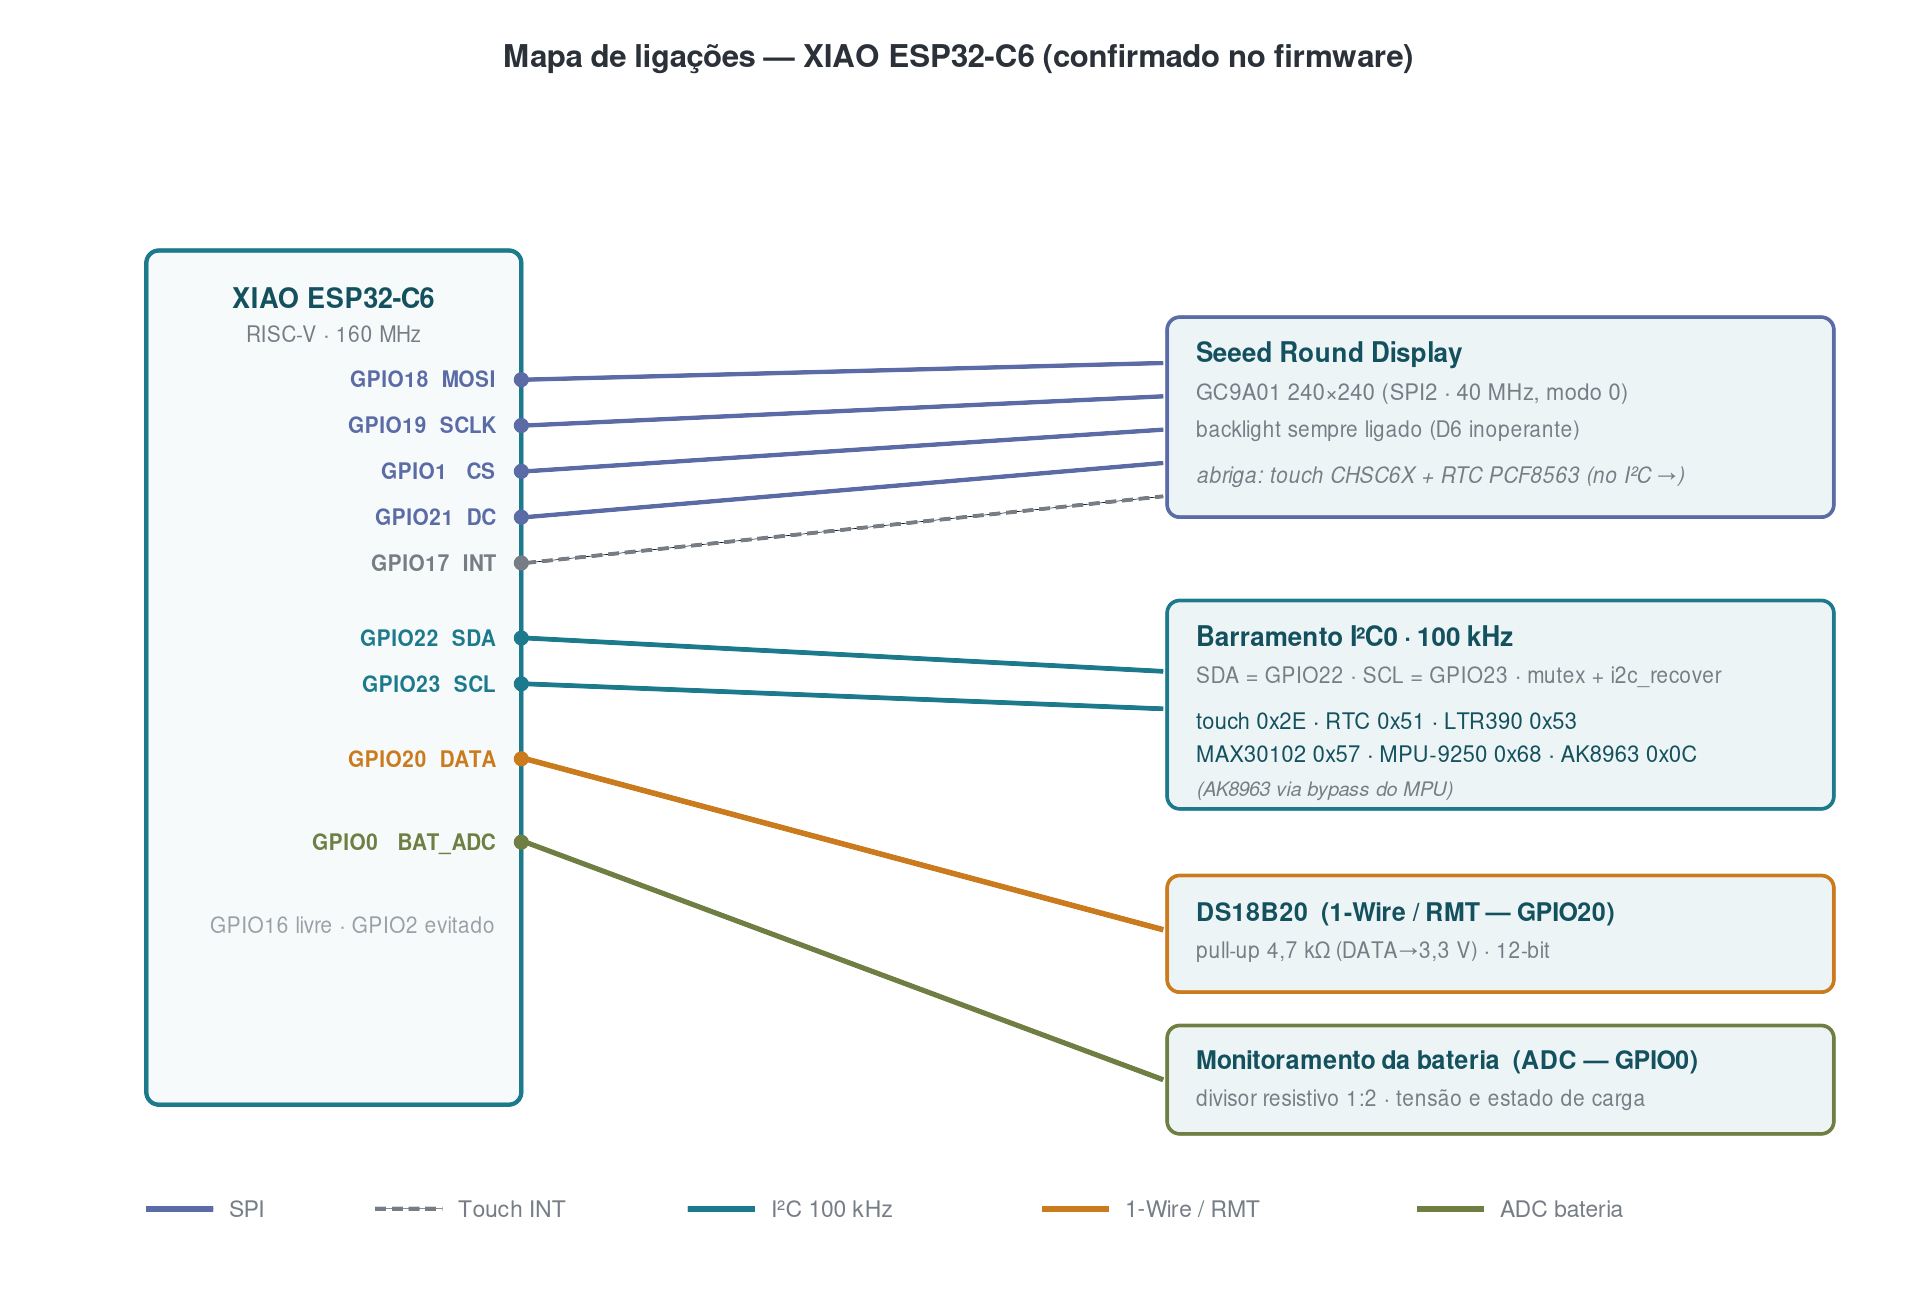
\includegraphics[width=0.95\textwidth]{Diagramas/sistema/mapa_ligacoes.png}
\fonteelemento{Elaborado pelo autor a partir do firmware integrado e do projeto da placa}
\end{figure}


Todos os m\'odulos compartilharam a refer\^encia de terra e foram alimentados em n\'iveis compat\'iveis com suas placas de conex\~ao. O esquema, o leiaute e a fotografia foram preservados como registros complementares da montagem utilizada.


\subsection{Metodologia de desenvolvimento}


\subsubsection{Levantamento de requisitos}


Os requisitos foram derivados do problema de integrar fun\c{c}\~oes independentes em uma plataforma vest\'ivel com recursos compartilhados. Foram definidos como requisitos funcionais a apresenta\c{c}\~ao de hora e data, a navega\c{c}\~ao por toque, a aquisi\c{c}\~ao dos sensores biom\'etricos, ambientais e inerciais e a apresenta\c{c}\~ao de suas informa\c{c}\~oes em telas pr\'oprias.


Os requisitos arquiteturais estabeleceram que cada fun\c{c}\~ao sensorial deveria ser encapsulada em um m\'odulo, que novos m\'odulos pudessem ser inclu\'idos com altera\c{c}\~oes localizadas e que a aus\^encia de um sensor n\~ao impedisse a continuidade das fun\c{c}\~oes independentes. O acesso concorrente ao I$^2$C deveria ser serializado, e erros de comunica\c{c}\~ao n\~ao poderiam provocar espera indefinida nem interromper deliberadamente toda a inicializa\c{c}\~ao.


Como restri\c{c}\~oes foram considerados o processamento em n\'ucleo \'unico, a mem\'oria dispon\'ivel, a parti\c{c}\~ao de aplica\c{c}\~ao de aproximadamente 1 MiB, o display circular de 240 $\times$ 240 pixels, a coexist\^encia de dispositivos no mesmo I$^2$C e a indisponibilidade de controle do backlight. Gerenciamento avan\c{c}ado de energia, valida\c{c}\~ao cl\'inica, persist\^encia do ped\^ometro, conectividade sem fio e compensa\c{c}\~ao de inclina\c{c}\~ao da b\'ussola foram exclu\'idos da vers\~ao avaliada.


\subsubsection{Crit\'erios de sele\c{c}\~ao de componentes}


A sele\c{c}\~ao partiu da necessidade de representar transportes e classes de sensoriamento diferentes em uma \'unica plataforma. O XIAO ESP32-C6 e o Round Display formaram a base pela compatibilidade mec\^anica, pelas dimens\~oes e pela disponibilidade dos perif\'ericos necess\'arios. O display circular, o toque e o RTC permitiram construir a interface demonstradora sem uma placa gr\'afica adicional.


O MAX30102 foi escolhido por integrar aquisi\c{c}\~ao PPG reflexiva em dois comprimentos de onda. O DS18B20 acrescentou um sensor digital em interface 1-Wire independente do I$^2$C. O LTR390 reuniu luz ambiente e ultravioleta em um \'unico dispositivo. O MPU-9250, com o AK8963, permitiu utilizar a mesma unidade para pedometria e orienta\c{c}\~ao magn\'etica.


Disponibilidade, documenta\c{c}\~ao e exist\^encia pr\'evia dos componentes tamb\'em influenciaram a escolha. N\~ao foi realizada compara\c{c}\~ao experimental sistem\'atica com microcontroladores ou sensores alternativos; portanto, a sele\c{c}\~ao representa uma decis\~ao de projeto segundo os requisitos e recursos dispon\'iveis, e n\~ao a demonstra\c{c}\~ao de superioridade desses componentes.


\subsubsection{Defini\c{c}\~ao da arquitetura}


A arquitetura foi definida pela separa\c{c}\~ao entre n\'ucleo da aplica\c{c}\~ao, servi\c{c}os compartilhados, drivers de hardware e m\'odulos funcionais. Cada m\'odulo foi concebido como uma unidade autocontida com opera\c{c}\~oes de inicializa\c{c}\~ao, cria\c{c}\~ao de tela e exibi\c{c}\~ao de tela. O n\'ucleo registra essas opera\c{c}\~oes e coordena a navega\c{c}\~ao sem incorporar o processamento espec\'ifico de cada sensor.


As aquisi\c{c}\~oes peri\'odicas foram atribu\'idas a tarefas independentes. Quando uma aquisi\c{c}\~ao s\'o era necess\'aria para atualizar uma tela, sua execu\c{c}\~ao foi condicionada \`a tela ativa. Servi\c{c}os comuns concentraram o acesso \`a interface gr\'afica, ao barramento I$^2$C e \`a persist\^encia em NVS. O contrato e as depend\^encias concretas da implementa\c{c}\~ao s\~ao apresentados no cap\'itulo de Desenvolvimento.


A extensibilidade foi considerada durante a defini\c{c}\~ao dos pontos de registro e das interfaces. A inicializa\c{c}\~ao n\~ao fatal e a recupera\c{c}\~ao do I$^2$C tamb\'em foram incorporadas \`a arquitetura. A avalia\c{c}\~ao desta vers\~ao combinou estudo retrospectivo de integra\c{c}\~ao, an\'alise est\'atica das depend\^encias e ensaios qualitativos com remo\c{c}\~ao individual e combinada dos sensores; a efic\'acia din\^amica da recupera\c{c}\~ao do barramento permaneceu fora do escopo experimental.


\subsubsection{Desenvolvimento incremental}


O desenvolvimento foi conduzido em etapas. Cada componente foi inicialmente estudado a partir da folha de dados e exercitado isoladamente, com inspe\c{c}\~ao de identifica\c{c}\~ao, configura\c{c}\~ao e dados brutos. Em seguida, sua aquisi\c{c}\~ao e seu processamento foram separados do c\'odigo de apresenta\c{c}\~ao, e o m\'odulo foi incorporado ao contrato comum da plataforma.


A integra\c{c}\~ao ocorreu progressivamente para permitir localizar conflitos de endere\c{c}amento, temporiza\c{c}\~ao, alimenta\c{c}\~ao e mem\'oria. Ap\'os cada inclus\~ao, foram verificados inicializa\c{c}\~ao, resposta da interface, logs de erro e continuidade das fun\c{c}\~oes j\'a existentes. Problemas observados durante essa evolu\c{c}\~ao orientaram a redu\c{c}\~ao do I$^2$C para 100 kHz, a serializa\c{c}\~ao por mutex, a recupera\c{c}\~ao p\'os-NACK, o aumento do pool do LVGL e o condicionamento das aquisi\c{c}\~oes pela tela ativa. A Figura~\ref{fig:metodo-incremental} sintetiza o ciclo aplicado.


\begin{figure}[H]
\centering
\caption{M\'etodo incremental de desenvolvimento e integra\c{c}\~ao}
\label{fig:metodo-incremental}
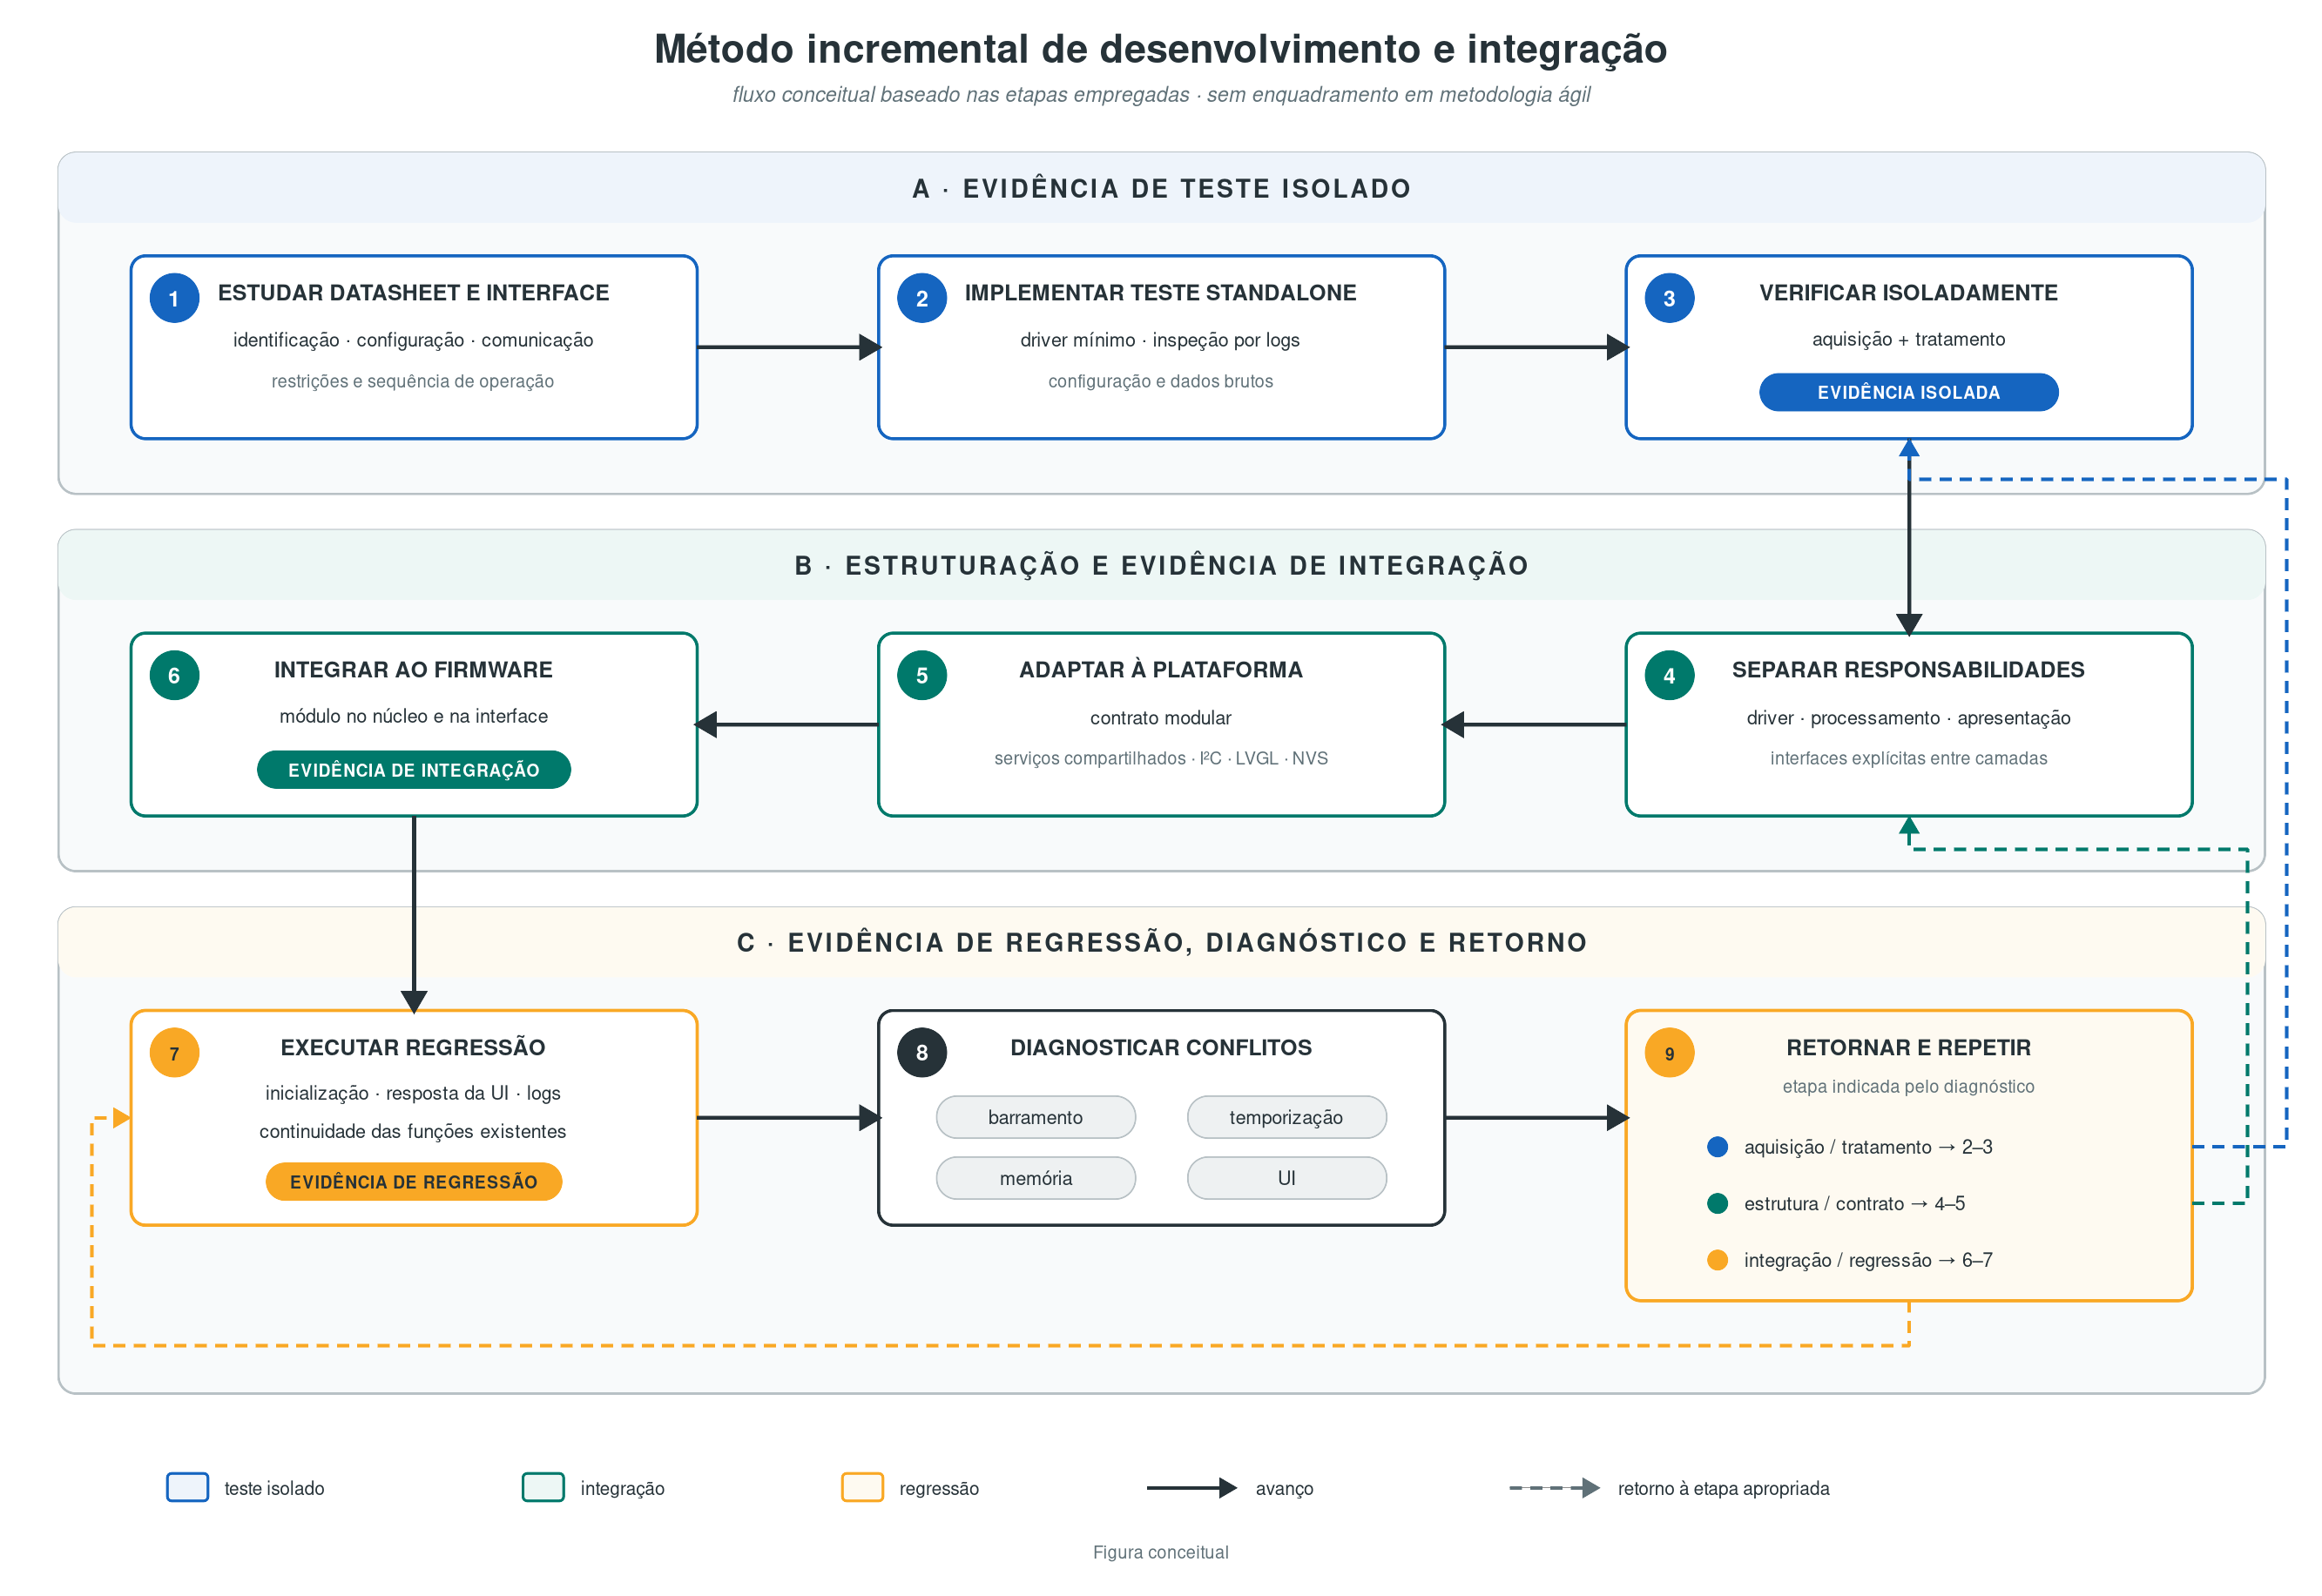
\includegraphics[width=0.96\textwidth]{Diagramas/teoricas/metodo_incremental.png}
\fonteelemento{Elaborado pelo autor a partir do procedimento empregado no projeto}
\end{figure}


As corre\c{c}\~oes realizadas durante o desenvolvimento n\~ao constituem, isoladamente, ensaios finais. Para que uma observa\c{c}\~ao de depura\c{c}\~ao seja apresentada como resultado, ela dever\'a ser repetida segundo um dos procedimentos definidos neste cap\'itulo e acompanhada de vers\~ao do firmware, condi\c{c}\~oes, dados e crit\'erio de interpreta\c{c}\~ao.


\subsubsection{Crit\'erios para drivers pr\'oprios e componentes oficiais}


Um componente oficial foi preferido quando oferecia compatibilidade com o ESP-IDF 5.5.1, utilizava as APIs atuais, apresentava manuten\c{c}\~ao e encapsulava adequadamente o perif\'erico sem impedir a integra\c{c}\~ao arquitetural. Esse crit\'erio foi aplicado ao controlador do display, \`a porta do LVGL, ao 1-Wire e ao DS18B20.


Drivers pr\'oprios foram empregados quando era necess\'ario controlar diretamente os registradores, adaptar o comportamento ao barramento compartilhado ou suprir a aus\^encia de componente compat\'ivel com o hardware e a API adotados. Eles foram limitados \`a comunica\c{c}\~ao e \`a configura\c{c}\~ao necess\'arias ao projeto, evitando reproduzir integralmente mapas de registradores no corpo do trabalho.


A decis\~ao entre reutiliza\c{c}\~ao e implementa\c{c}\~ao pr\'opria n\~ao foi usada como medida de qualidade. Em ambos os casos, a integra\c{c}\~ao deveria oferecer tratamento expl\'icito de erro, limites de espera e uma interface est\'avel para o m\'odulo funcional.


\subsubsection{Tratamento de falhas}


A inicializa\c{c}\~ao de cada m\'odulo foi projetada para retornar seu estado ao n\'ucleo. Uma falha deveria marcar somente o m\'odulo dependente como indispon\'ivel e permitir que a sequ\^encia prosseguisse. A interface deveria comunicar a indisponibilidade sem executar acessos repetidos a um dispositivo que n\~ao respondeu durante a inicializa\c{c}\~ao.


O I$^2$C compartilhado foi protegido por mutex com heran\c{c}a de prioridade. Cada transa\c{c}\~ao recebeu limite de espera e retorno de erro. Ap\'os NACK ou condi\c{c}\~ao que deixasse o barramento sem progresso, o servi\c{c}o poderia executar a recupera\c{c}\~ao por reset do barramento antes de uma tentativa controlada posterior. Um scanner executado no boot forneceu diagn\'ostico dos endere\c{c}os presentes.


O tratamento foi orientado \`a conten\c{c}\~ao: n\~ao se pressup\^os que toda falha pudesse ser corrigida. Se um sensor continuasse ausente, as fun\c{c}\~oes que dependiam dele permaneceriam indispon\'iveis, enquanto o rel\'ogio, a interface e os m\'odulos independentes deveriam continuar operando.


\subsubsection{Crit\'erios de aceita\c{c}\~ao}


Os crit\'erios de aceita\c{c}\~ao foram divididos em tr\^es n\'iveis. No n\'ivel funcional, cada m\'odulo deveria inicializar quando seu hardware estivesse presente, produzir dados ou estados coerentes com o est\'imulo aplicado e atualizar sua tela sem bloquear a navega\c{c}\~ao. Esse n\'ivel n\~ao equivale a valida\c{c}\~ao quantitativa da grandeza medida.


No n\'ivel de integra\c{c}\~ao, o sistema deveria inicializar todos os m\'odulos dispon\'iveis, preservar transa\c{c}\~oes at\^omicas no I$^2$C, manter a interface responsiva e continuar executando fun\c{c}\~oes independentes diante da aus\^encia de um sensor. N\~ao deveriam ocorrer reinicializa\c{c}\~ao espont\^anea, disparo de watchdog ou crescimento cont\'inuo de uso de mem\'oria durante o intervalo de ensaio.


No n\'ivel arquitetural, a inclus\~ao de um m\'odulo deveria ocorrer por meio do contrato definido, com altera\c{c}\~oes localizadas e registradas. A matriz de depend\^encias deveria permitir identificar rela\c{c}\~oes entre n\'ucleo, servi\c{c}os, drivers e m\'odulos sem acesso cruzado n\~ao documentado. Como n\~ao foram fixados limites quantitativos de CPU, heap, boot ou erro sensorial, as medidas dispon\'iveis foram interpretadas de forma descritiva e comparativa.


\subsection{Metodologia dos ensaios}


Foram executados os ensaios funcionais dos sensores, do RTC e do consumo de corrente, a an\'alise estrutural de extensibilidade e acoplamento, a medi\c{c}\~ao est\'atica do sistema integrado e um piloto de inicializa\c{c}\~ao degradada. N\~ao foram realizadas as compila\c{c}\~oes incrementais por m\'odulo, as medidas din\^amicas de CPU e heap, a s\'erie controlada de tempo de boot, a falha I$^2$C induzida nem um ensaio prolongado com roteiro completo de navega\c{c}\~ao. A Figura~\ref{fig:instrumentacao-ensaios} distingue conex\~oes f\'isicas de rela\c{c}\~oes de observa\c{c}\~ao e compara\c{c}\~ao.


\begin{figure}[H]
\centering
\caption{Instrumenta\c{c}\~ao empregada nos ensaios do prot\'otipo}
\label{fig:instrumentacao-ensaios}
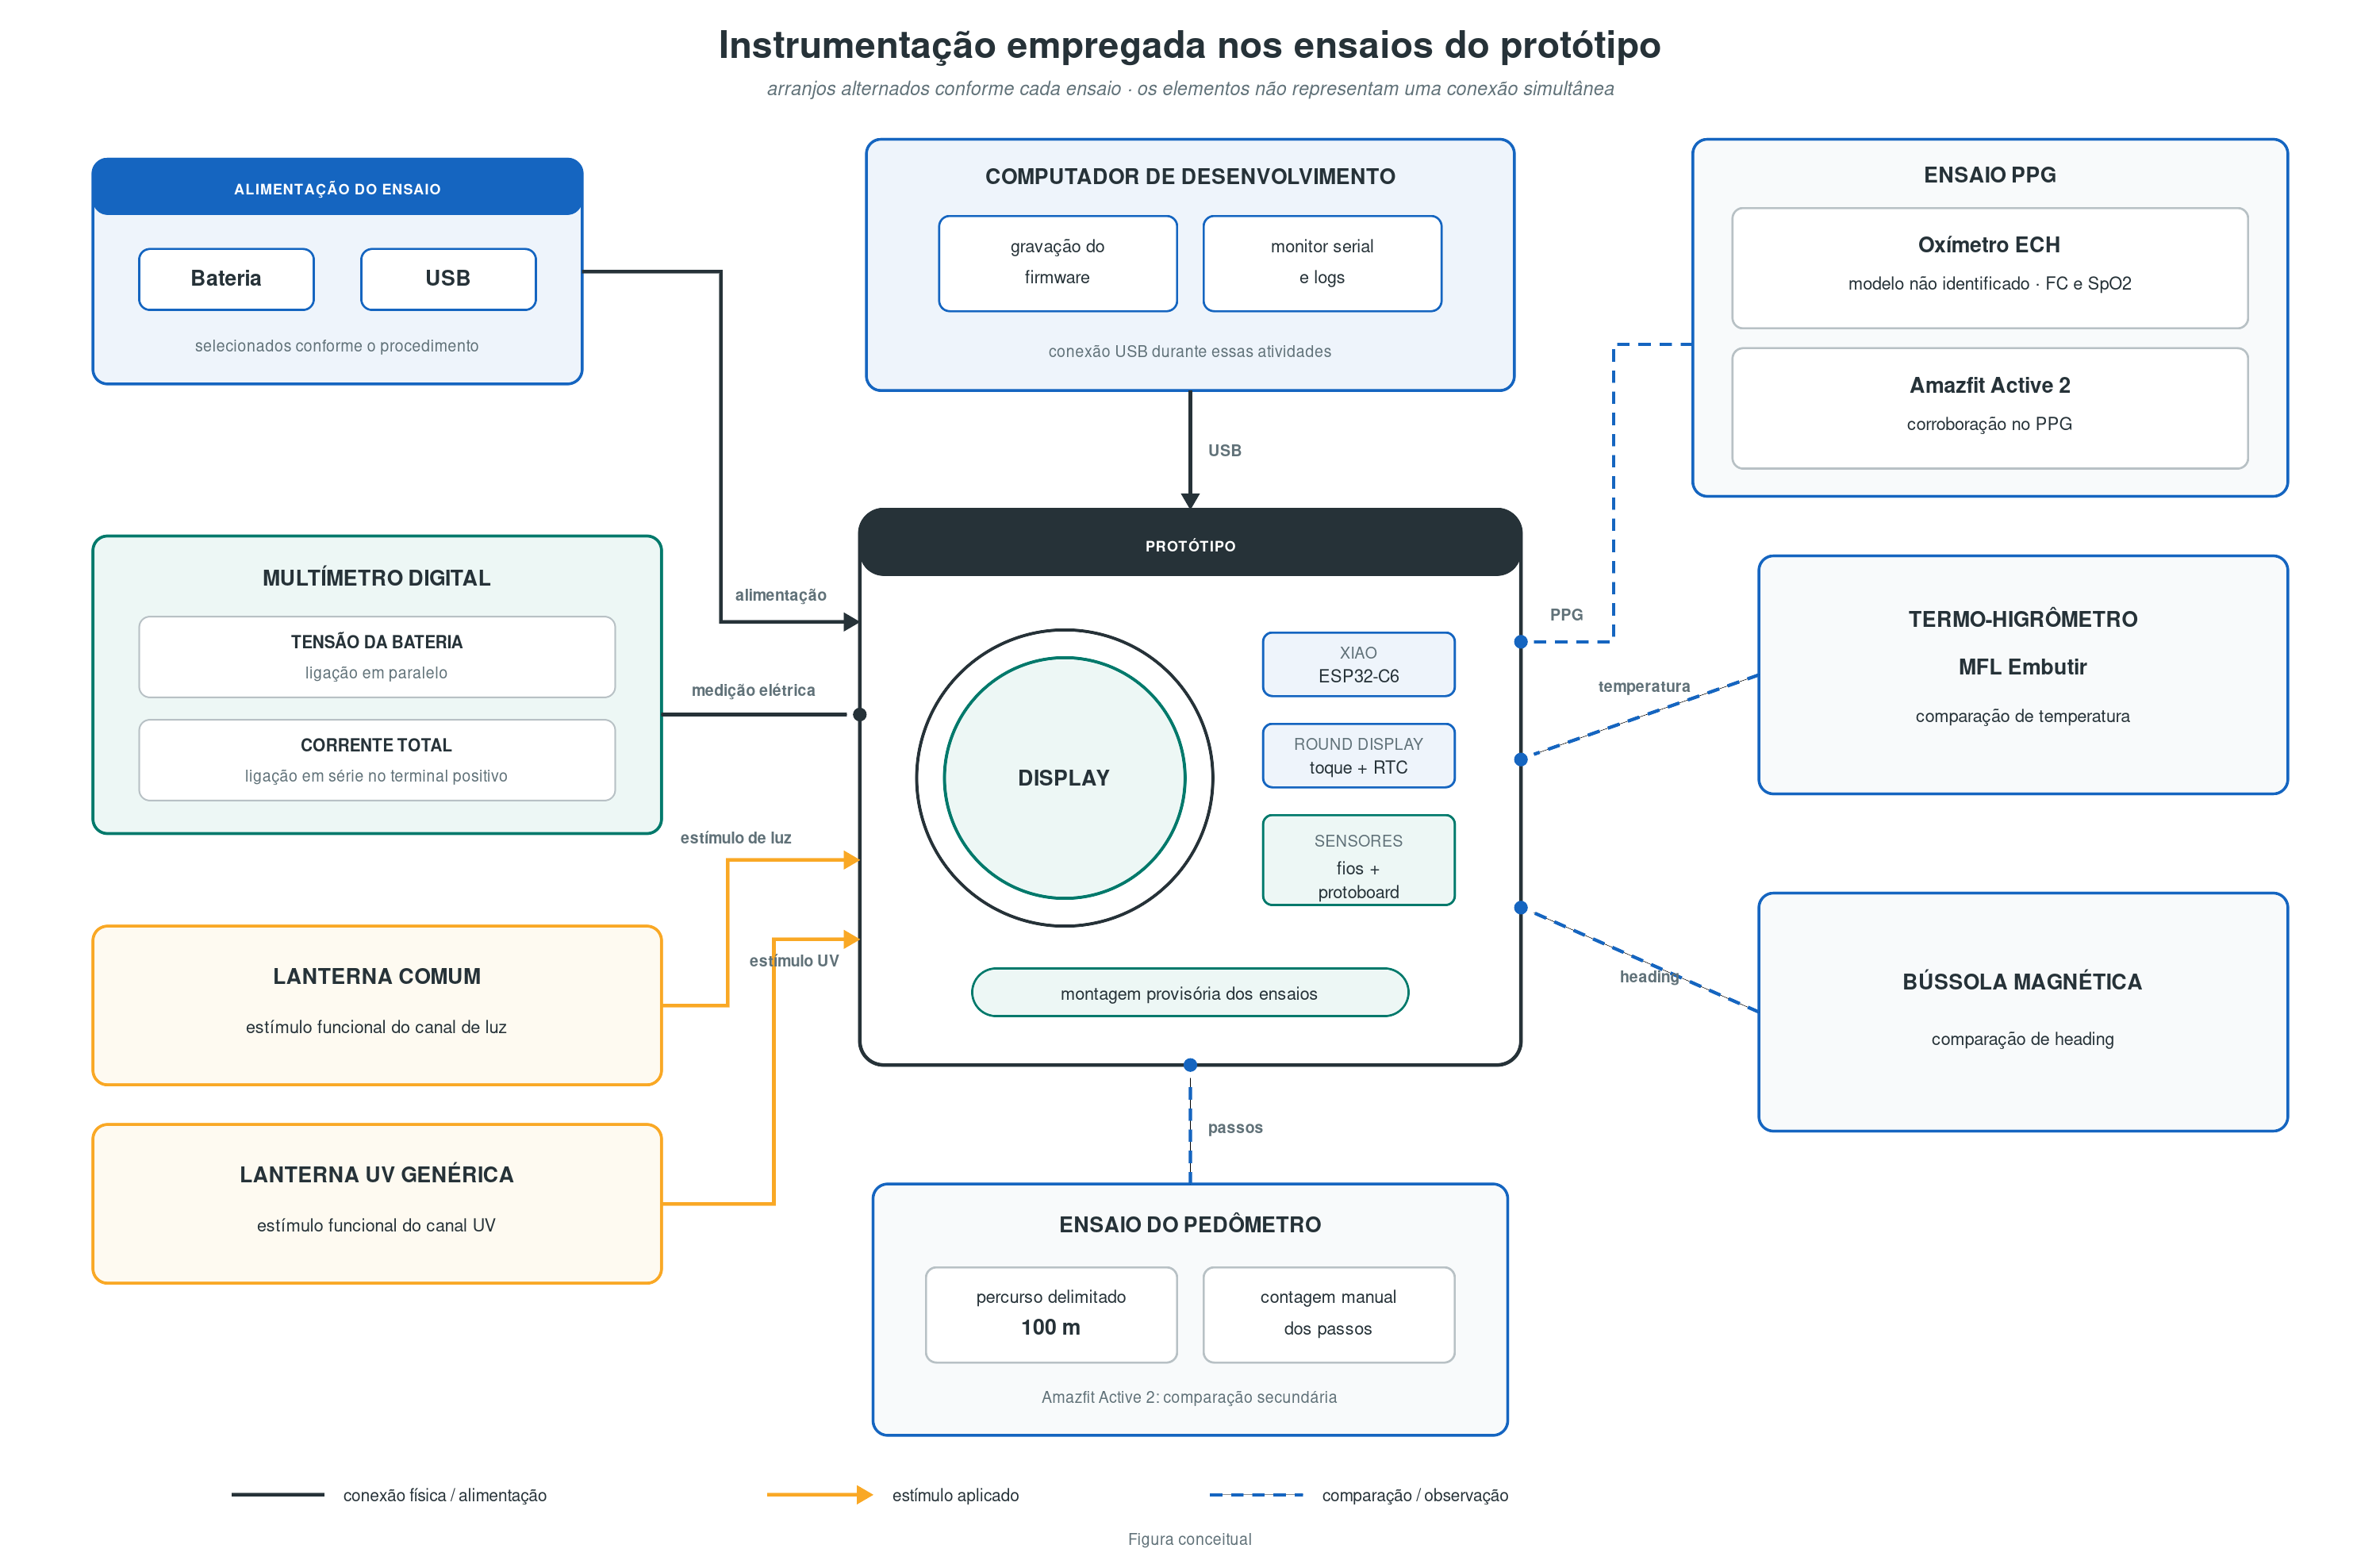
\includegraphics[width=0.96\textwidth]{Diagramas/teoricas/instrumentacao_ensaios.png}
\fonteelemento{Elaborado pelo autor a partir do caderno de ensaios}
\end{figure}


\subsubsection{Condi\c{c}\~oes comuns e rastreabilidade}


Cada coleta registrou, quando dispon\'iveis, data, local, vers\~ao do hardware, identifica\c{c}\~ao do firmware, configura\c{c}\~ao de compila\c{c}\~ao, forma de alimenta\c{c}\~ao, instrumentos, dura\c{c}\~ao e operador. Os dados brutos foram preservados em formato tabular quando houve exporta\c{c}\~ao, acompanhados do script ou procedimento usado para produzir tabelas e gr\'aficos. Lacunas desses metadados foram mantidas como limita\c{c}\~oes, sem reconstru\c{c}\~ao retrospectiva.


O n\'umero efetivo de repeti\c{c}\~oes foi informado para cada ensaio. S\'eries com uma ou duas execu\c{c}\~oes foram classificadas como pilotos ou testes funcionais limitados, e n\~ao como caracteriza\c{c}\~ao estat\'istica. Eventos inesperados, amostras descartadas e crit\'erios de exclus\~ao foram preservados no caderno de ensaios.


\subsubsection{Extensibilidade}

Como a integra\c{c}\~ao de outro componente n\~ao integrou o escopo temporal da avalia\c{c}\~ao, a extensibilidade foi examinada por estudo retrospectivo da transforma\c{c}\~ao do teste standalone do MAX30102 em m\'odulo da plataforma. Foram identificados os arquivos reutilizados, criados e modificados, as adapta\c{c}\~oes ao barramento e ao mutex compartilhados, os pontos de registro no n\'ucleo e as altera\c{c}\~oes exigidas em componentes independentes.


A an\'alise considerou o confinamento das altera\c{c}\~oes ao driver e ao m\'odulo, a quantidade de pontos de registro no n\'ucleo e a ocorr\^encia de modifica\c{c}\~oes em fun\c{c}\~oes independentes. Essa evid\^encia \'e estrutural: ela descreve o caso observado e n\~ao representa uma medida geral do tempo necess\'ario para integrar qualquer sensor.


\subsubsection{Acoplamento}


O acoplamento foi avaliado sobre a mesma vers\~ao do firmware utilizada nos demais ensaios arquiteturais. Foi constru\'ida uma matriz de depend\^encias entre n\'ucleo, servi\c{c}os, drivers e m\'odulos a partir de inclus\~oes de cabe\c{c}alhos, chamadas p\'ublicas, acesso a vari\'aveis globais e uso de recursos compartilhados.


Para cada par de componentes, foram registradas a presen\c{c}a e a dire\c{c}\~ao da depend\^encia. Chamadas realizadas por interfaces previstas no contrato foram diferenciadas de acessos diretos a dados internos ou de chamadas entre m\'odulos funcionais. A leitura conjunta do grafo e da matriz foi empregada para identificar concentra\c{c}\~oes e ciclos, sem reduzir a avalia\c{c}\~ao a uma \'unica contagem.


\subsubsection{Mem\'oria}


O uso est\'atico de mem\'oria foi obtido para uma compila\c{c}\~ao limpa do sistema integrado, por meio das ferramentas de an\'alise do ESP-IDF. Foram registrados o tamanho da imagem da aplica\c{c}\~ao e a ocupa\c{c}\~ao da parti\c{c}\~ao configurada.


N\~ao foram produzidas compila\c{c}\~oes controladas com habilita\c{c}\~ao incremental dos m\'odulos nem uma s\'erie de heap por cen\'ario. Por isso, o resultado caracteriza somente a configura\c{c}\~ao integrada e n\~ao permite atribuir um custo de mem\'oria isolado a cada m\'odulo.


\subsubsection{CPU}

A vers\~ao corrente possui um contador associado ao \emph{idle hook}, mas n\~ao foi executada uma s\'erie controlada com linha de base congelada e cen\'arios repetidos. Assim, registros explorat\'orios de ociosidade n\~ao foram empregados como medida de carga de CPU.


A caracteriza\c{c}\~ao futura dever\'a amostrar o contador em janelas fixas, estabelecer uma refer\^encia reproduz\'ivel e registrar simultaneamente heap livre e menor heap observado. Mesmo nessas condi\c{c}\~oes, o m\'etodo fornecer\'a uma estimativa global, sem separar o consumo por tarefa nem demonstrar atendimento a prazos.


\subsubsection{Tempo de boot}


Os logs de inicializa\c{c}\~ao foram usados para confirmar a sequ\^encia de cria\c{c}\~ao dos servi\c{c}os e dos m\'odulos e a continuidade do boot em condi\c{c}\~ao degradada. N\~ao foi definida uma origem f\'isica de tempo nem executada uma s\'erie repetida at\'e a disponibiliza\c{c}\~ao da interface.


Consequentemente, os registros permitem discutir ordem e toler\^ancia a falhas, mas n\~ao constituem medida de tempo de boot. Uma caracteriza\c{c}\~ao quantitativa exigir\'a evento inicial observ\'avel, crit\'erio final fixo, repeti\c{c}\~oes e resolu\c{c}\~ao temporal conhecida.


\subsubsection{Robustez do I$^2$C}


A robustez foi examinada por an\'alise est\'atica dos caminhos de erro, dos limites de espera e do mecanismo de recupera\c{c}\~ao, complementada pelos registros de integra\c{c}\~ao. O firmware serializa as transa\c{c}\~oes, propaga o erro e pode reinicializar o barramento ap\'os falha.


N\~ao foi executada uma s\'erie de falhas induzidas com medi\c{c}\~ao do tempo de recupera\c{c}\~ao e contabiliza\c{c}\~ao de sucessos. Portanto, a presen\c{c}a do mecanismo foi confirmada, mas sua efic\'acia din\^amica n\~ao foi quantificada.


\subsubsection{Sensor ausente}


Com o prot\'otipo desligado, cada sensor externo foi removido individualmente e o sistema foi religado. O procedimento tamb\'em foi repetido com sensores removidos em diversos arranjos. Em cada condi\c{c}\~ao, foram conferidos o t\'ermino da inicializa\c{c}\~ao, a tela principal, o toque, o RTC, a navega\c{c}\~ao pelos menus, a indica\c{c}\~ao de indisponibilidade da fun\c{c}\~ao dependente e o acesso aos demais m\'odulos conectados.


O ensaio teve car\'ater funcional e qualitativo: verificou se a aus\^encia de um ou mais sensores impedia o uso do restante do prot\'otipo, sem medir tempo de recupera\c{c}\~ao nem produzir uma taxa estat\'istica de disponibilidade.


\subsubsection{Ensaio prolongado}


Foi mantida uma observa\c{c}\~ao prolongada da tela principal para verificar continuidade visual e atualiza\c{c}\~ao do rel\'ogio. A dura\c{c}\~ao exata e um roteiro completo de altern\^ancia entre m\'odulos n\~ao foram preservados no registro.


Essa observa\c{c}\~ao sustenta apenas a continuidade no intervalo acompanhado. Ela n\~ao substitui um ensaio prolongado com dura\c{c}\~ao definida, navega\c{c}\~ao repet\'ivel, contadores de erro, heap e condi\c{c}\~oes ambientais registrados.


\subsubsection{MAX30102}

O ensaio funcional do MAX30102 foi executado no firmware standalone durante aproximadamente 65 s, com aquisi\c{c}\~ao a 100 Hz e sa\'ida resumida a cada segundo. Um ox\'imetro de dedo ECH e um Amazfit Active 2 foram usados simultaneamente; a an\'alise quantitativa tomou o ox\'imetro como comparador e usou o dispositivo comercial apenas como corrobora\c{c}\~ao. A configura\c{c}\~ao standalone e suas diferen\c{c}as em rela\c{c}\~ao ao firmware integrado foram registradas.


Foram registrados valores de frequ\^encia card\'iaca e SpO$_2$ ao longo de trechos temporais compar\'aveis. Os canais vermelho e infravermelho brutos foram exportados a 50 Hz, enquanto o processamento permaneceu configurado para aquisi\c{c}\~ao a 100 Hz. O transiente inicial foi separado e os sinais bruto, sem componente DC e filtrado foram produzidos por script a partir do arquivo preservado.


As leituras dos tr\^es dispositivos foram aproximadas no tempo pela observa\c{c}\~ao simult\^anea, sem rel\'ogio eletr\^onico compartilhado. A compara\c{c}\~ao foi classificada como teste funcional limitado e n\~ao como valida\c{c}\~ao cl\'inica.


\subsubsection{DS18B20}

O DS18B20 foi mantido ao lado do termo-higr\^ometro MFL Embutir durante aproximadamente 5 min em ambiente pr\'oximo de 23 $^\circ$C. Ambos permaneceram em posi\c{c}\~ao fixa; a compara\c{c}\~ao foi limitada a um ponto de opera\c{c}\~ao e classificada como verifica\c{c}\~ao de plausibilidade.


Para observar resposta transit\'oria, o prot\'otipo foi colocado em freezer com a porta fechada por 2 min, com registro ap\'os 1 e 2 min. Em ensaio separado, o probe foi aproximado da maior boca de um fog\~ao por 30 s e o aquecimento foi interrompido ao atingir 70 $^\circ$C para preservar o encapsulamento. Como n\~ao houve refer\^encia calibrada nesses transientes, o procedimento avaliou somente resposta funcional.


\subsubsection{LTR390}


Ilumin\^ancia e ultravioleta foram exercitados separadamente. Na vers\~ao integrada, cada troca de modo descarta tr\^es amostras de estabiliza\c{c}\~ao e mant\'em estados de filtragem independentes para ALS e UVS.


Para ilumin\^ancia, o sensor foi exposto a obstru\c{c}\~ao total, ambiente interno, lanterna comum, c\'eu nublado e luz solar direta. Como n\~ao havia lux\'imetro identificado, o procedimento verificou ordena\c{c}\~ao qualitativa da resposta e ocorr\^encia de satura\c{c}\~ao, sem validar quantitativamente a unidade lux.


Para UVI, a leitura externa foi comparada com uma refer\^encia meteorol\'ogica correspondente ao local e ao dia. Essa fonte n\~ao equivalia a um radi\^ometro colocado junto ao prot\'otipo e foi usada somente como contexto de plausibilidade.

Em teste standalone adicional, uma lanterna UV gen\'erica foi aproximada de cerca de 20 cm at\'e muito pr\'oximo do sensor. Esse procedimento avaliou somente se a indica\c{c}\~ao aumentava com a aproxima\c{c}\~ao da fonte, pois seu espectro e irradi\^ancia n\~ao eram conhecidos.


\subsubsection{B\'ussola}

Antes da coleta, a calibra\c{c}\~ao em 12 setores foi executada no pr\'oprio dispositivo. O prot\'otipo e a b\'ussola Norvix DC45-2 foram mantidos no mesmo plano horizontal, sem ajuste de declina\c{c}\~ao. Foram comparadas duas orienta\c{c}\~oes separadas por aproximadamente meia-volta.


A diferen\c{c}a foi calculada diretamente entre as indica\c{c}\~oes magn\'eticas. Como foram avaliadas apenas duas orienta\c{c}\~oes e a refer\^encia n\~ao era calibrada, o ensaio foi tratado como teste funcional de resposta direcional, sem alega\c{c}\~ao de precis\~ao.


\subsubsection{Ped\^ometro}

O ensaio controlado utilizou um percurso de 100 m delimitado pela ferramenta de medi\c{c}\~ao do Google Maps. Um participante percorreu o trecho na ida e na volta em ritmo habitual, com o prot\'otipo e o Amazfit Active 2 no pulso. Os passos foram contados manualmente e adotados como refer\^encia.


Para cada percurso foram registrados passos de refer\^encia, passos detectados pelo prot\'otipo e passos informados pelo dispositivo comercial. Foram calculados erro absoluto e erro relativo. O ensaio foi limitado a um participante, um ritmo e duas repeti\c{c}\~oes.


\[
E_{\mathrm{abs}}=N_{\mathrm{detectado}}-N_{\mathrm{referencia}},
\qquad
E_{\mathrm{rel}}=\frac{|E_{\mathrm{abs}}|}{N_{\mathrm{referencia}}}\times 100\%.
\]


O contador foi reiniciado antes de cada repeti\c{c}\~ao, pois sua persist\^encia n\~ao faz parte da implementa\c{c}\~ao. Os resultados foram limitados \`as condi\c{c}\~oes e ao posicionamento ensaiados.


\subsubsection{Bateria}

A tens\~ao indicada pelo ADC foi comparada com o mult\'imetro nas condi\c{c}\~oes com USB e somente com bateria. Em ensaio separado, o mult\'imetro foi ligado em s\'erie com o terminal positivo da bateria e a corrente foi observada em nove cen\'arios funcionais ap\'os intervalo de estabiliza\c{c}\~ao.

N\~ao foi executada curva de descarga completa. A autonomia foi apenas estimada pela raz\~ao entre uma capacidade \`util assumida de aproximadamente 1000 mAh e as correntes observadas. Esses valores n\~ao foram apresentados como autonomia medida, e as proje\c{c}\~oes com modos de baixo consumo foram reservadas aos trabalhos futuros.

\clearpage
\section{Desenvolvimento e Implementa\c{c}\~ao}


Este cap\'itulo apresenta a implementa\c{c}\~ao da plataforma, desde a organiza\c{c}\~ao dos recursos f\'isicos at\'e a integra\c{c}\~ao dos m\'odulos funcionais. A descri\c{c}\~ao foi conferida diretamente na vers\~ao corrente do firmware em \texttt{Codigos/IDroid/main}; documentos hist\'oricos foram usados apenas para contextualizar decis\~oes de desenvolvimento e n\~ao como autoridade sobre a vers\~ao integrada.


\subsection{Vis\~ao geral do sistema}


A plataforma foi organizada em quatro n\'iveis: hardware, drivers, servi\c{c}os compartilhados e m\'odulos funcionais. O hardware re\'une o XIAO ESP32-C6, o Round Display e os sensores. Os drivers encapsulam os protocolos e registradores de cada dispositivo. Os servi\c{c}os coordenam recursos utilizados por mais de um m\'odulo, como I$^2$C, LVGL e NVS. Os m\'odulos associam aquisi\c{c}\~ao, processamento, estado funcional e tela.


A Figura~\ref{fig:arquitetura-implementada} sintetiza os componentes confirmados e as dire\c{c}\~oes de controle, dados e acesso ao hardware.


\begin{figure}[H]
\centering
\caption{Arquitetura de componentes da plataforma implementada}
\label{fig:arquitetura-implementada}
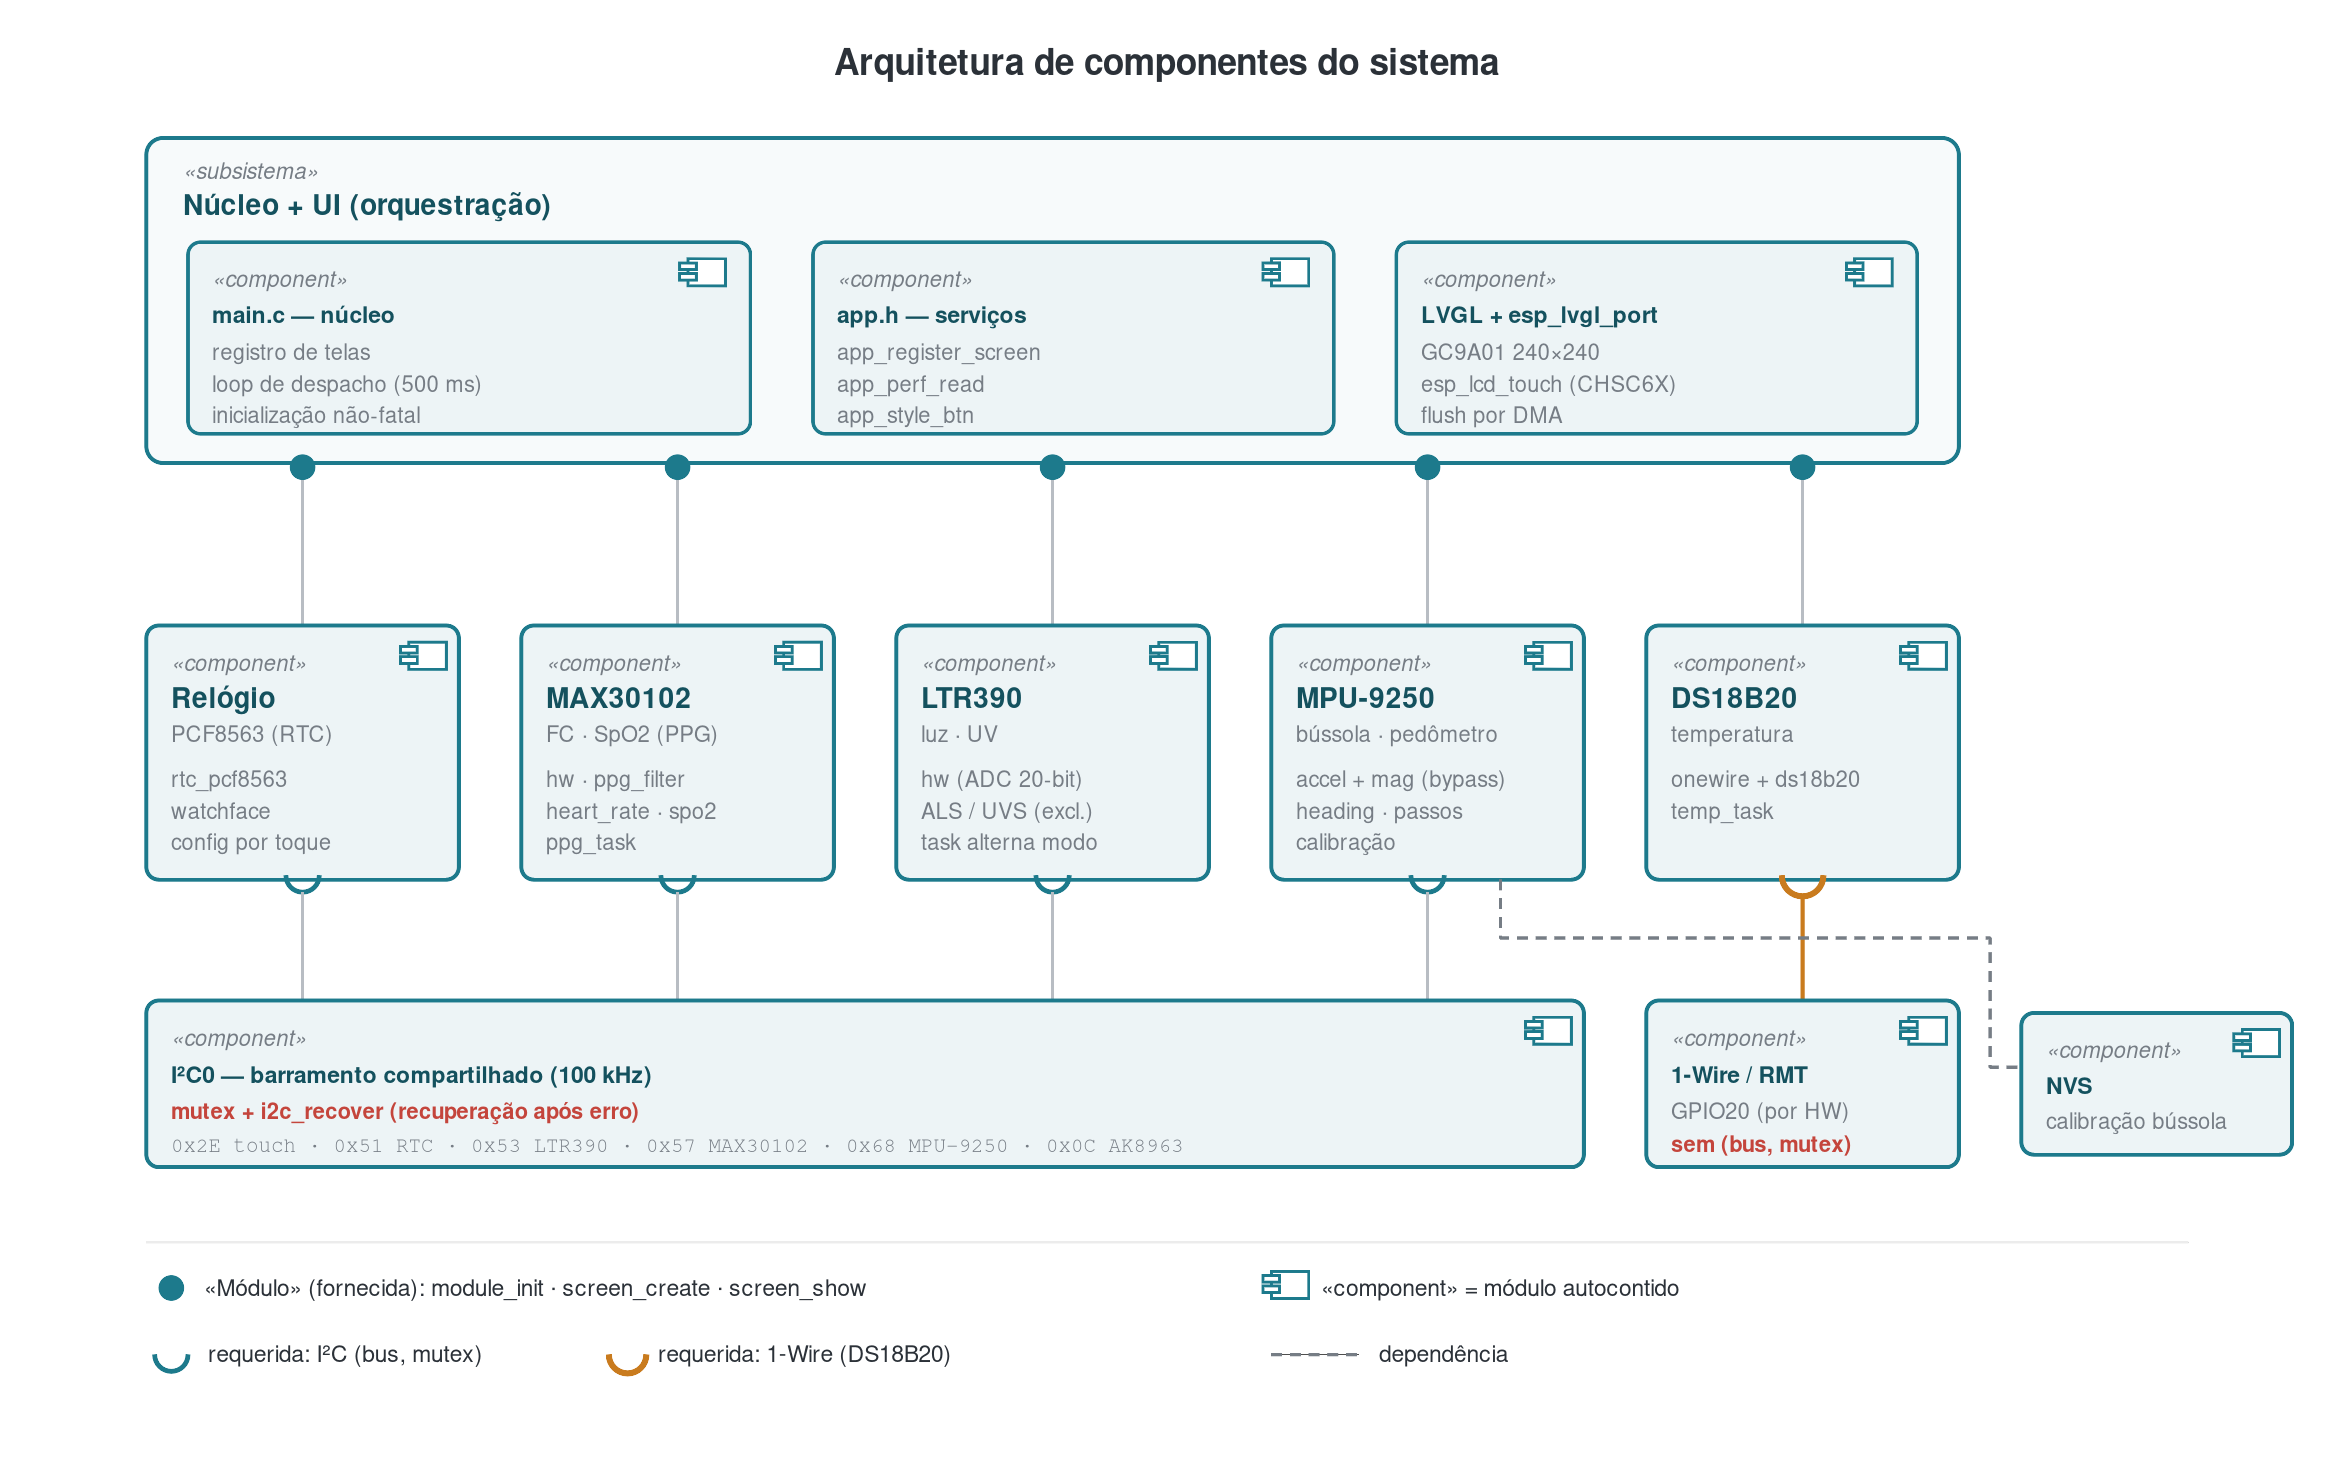
\includegraphics[width=0.96\textwidth]{Diagramas/sistema/arquitetura_componentes_sistema.png}
\fonteelemento{Elaborado pelo autor a partir do firmware integrado}
\end{figure}


O n\'ucleo n\~ao executa os algoritmos de cada sensor. Ele inicializa os servi\c{c}os, solicita a inicializa\c{c}\~ao dos m\'odulos, cria as telas e despacha a atualiza\c{c}\~ao correspondente \`a tela ativa. A aquisi\c{c}\~ao peri\'odica permanece nas tarefas dos m\'odulos, enquanto a LVGL \'e manipulada segundo o mecanismo de exclus\~ao fornecido por sua porta para o ESP-IDF.


\subsection{Arquitetura de hardware}


\subsubsection{Barramento I$^2$C compartilhado}


O I$^2$C foi criado uma \'unica vez pelo n\'ucleo com a API mestre introduzida nas vers\~oes recentes do ESP-IDF. O barramento opera a 100 kHz em SDA GPIO22 e SCL GPIO23. Cada driver registra seu dispositivo l\'ogico nessa inst\^ancia, em vez de criar um controlador pr\'oprio.


Seis endere\c{c}os coexistem no barramento: CHSC6X em 0x2E, PCF8563 em 0x51, LTR390 em 0x53, MAX30102 em 0x57, MPU-9250 em 0x68 e AK8963 em 0x0C. O \'ultimo torna-se acess\'ivel externamente quando o MPU-9250 \'e colocado em modo \emph{bypass}. Embora perten\c{c}am ao mesmo encapsulamento funcional, MPU-9250 e AK8963 constituem alvos I$^2$C distintos.


A frequ\^encia de 100 kHz foi adotada na integra\c{c}\~ao, substituindo configura\c{c}\~oes mais altas usadas em testes isolados. A redu\c{c}\~ao aumenta a margem para os tempos de subida na montagem com fios e m\'ultiplas placas. Como todos os dispositivos compartilham o controlador e as linhas, a coordena\c{c}\~ao por software e a recupera\c{c}\~ao do barramento foram tratadas como servi\c{c}os sist\^emicos.


\subsubsection{Interface SPI}


O display GC9A01A utiliza o perif\'erico SPI2 a 40 MHz. As linhas de clock e dados s\~ao compartilh\'aveis com o slot microSD do Round Display, enquanto sinais de sele\c{c}\~ao independentes delimitam as transa\c{c}\~oes. O firmware integrado utiliza o controlador de LCD disponibilizado como componente do ecossistema ESP-IDF; o cart\~ao n\~ao integra as fun\c{c}\~oes avaliadas.


As transfer\^encias gr\'aficas s\~ao predominantemente unidirecionais, do ESP32-C6 para o controlador. O uso de DMA pela porta gr\'afica permite transferir blocos de pixels sem movimenta\c{c}\~ao individual pela CPU. O acesso ao display permanece encapsulado pelo driver e pela LVGL, de modo que m\'odulos funcionais criam objetos gr\'aficos sem iniciar transa\c{c}\~oes SPI diretamente.


\subsubsection{Interface 1-Wire/RMT}


O DS18B20 utiliza uma interface separada, no GPIO20, com resistor de \emph{pull-up} externo. Os intervalos do protocolo 1-Wire s\~ao produzidos e amostrados por meio do perif\'erico RMT. Essa solu\c{c}\~ao reduz a depend\^encia de atrasos ativos em software e evita que a temporiza\c{c}\~ao de cada bit dependa diretamente da execu\c{c}\~ao cont\'inua de uma tarefa.


Foram reutilizados os componentes oficiais \texttt{onewire\_bus} e \texttt{ds18b20}. O m\'odulo de temperatura recebe valores j\'a convertidos pela API do componente e n\~ao conhece a representa\c{c}\~ao dos s\'imbolos do RMT. A separa\c{c}\~ao demonstra que o contrato funcional n\~ao exige que todos os m\'odulos utilizem o mesmo transporte.


\subsubsection{Alimenta\c{c}\~ao}


O prot\'otipo pode ser alimentado por USB por meio do XIAO ESP32-C6 ou por bateria conectada ao circuito do Round Display. A vers\~ao implementada n\~ao inclui gerenciamento avan\c{c}ado de energia, e o backlight permanece ligado durante a opera\c{c}\~ao. Recursos de suspens\~ao profunda, controle de brilho e otimiza\c{c}\~ao de autonomia n\~ao fazem parte do desenvolvimento descrito.

A leitura da tens\~ao da bateria tamb\'em integra a vers\~ao final. O positivo ap\'os a chave alimenta um divisor 1:2 formado por dois resistores de $100~\mathrm{k}\Omega$; o ponto m\'edio segue para o GPIO0/A0 do XIAO ESP32-C6. O firmware aplica calibra\c{c}\~ao do ADC, m\'edia de 16 amostras e suaviza\c{c}\~ao temporal antes de apresentar o estado estimado. A Figura~\ref{fig:divisor-bateria-xiao} mostra o circuito efetivamente empregado. Como a estimativa se baseia em tens\~ao, ela n\~ao equivale a um contador de carga.

\begin{figure}[H]
\centering
\caption{Divisor resistivo empregado na leitura da tens\~ao da bateria}
\label{fig:divisor-bateria-xiao}
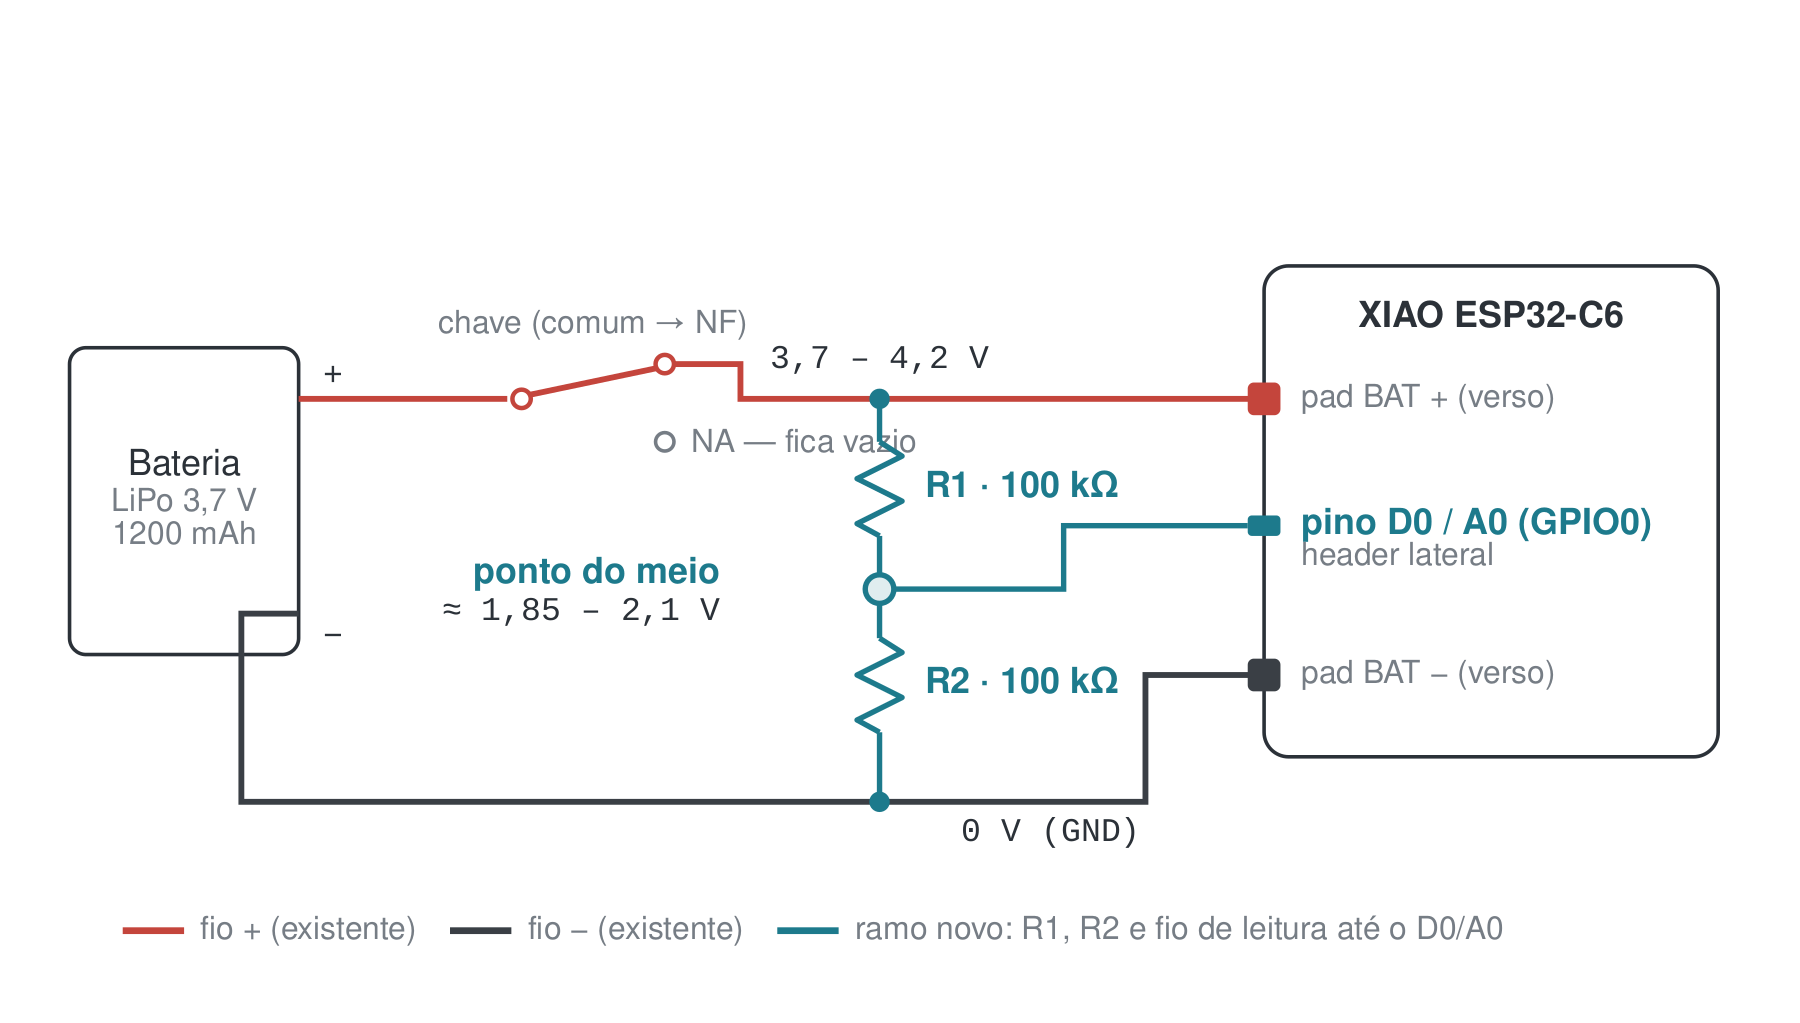
\includegraphics[width=0.90\textwidth]{Diagramas/bateria/divisor_bateria_xiao.png}
\fonteelemento{Elaborado pelo autor a partir do circuito implementado e de \texttt{bateria.c}}
\end{figure}


Durante a integra\c{c}\~ao, a alimenta\c{c}\~ao do MAX30102 exigiu aten\c{c}\~ao por causa dos pulsos de corrente dos emissores. Os testes A/B registrados no pr\'oprio c\'odigo associaram a configura\c{c}\~ao anterior, de aproximadamente 14,2 mA por emissor, a afundamento da linha de 3,3 V e travamento do I$^2$C na placa final. A configura\c{c}\~ao integrada passou a empregar o valor 0x24, correspondente a aproximadamente 7,2 mA por emissor.


\subsubsection{Placa prot\'otipo e inv\'olucro}


A integra\c{c}\~ao deixou a protoboard de desenvolvimento e foi transferida para uma placa prot\'otipo autoral, cujo esquema, leiaute, renderiza\c{c}\~oes e registro fotogr\'afico foram preservados. Um inv\'olucro tamb\'em foi fabricado por impress\~ao 3D para acomodar o conjunto. Esses elementos pertencem \`a implementa\c{c}\~ao realizada; revis\~oes futuras podem aprimor\'a-los, mas n\~ao correspondem a atividades pendentes de constru\c{c}\~ao.


\subsection{Arquitetura de software}


\subsubsection{Organiza\c{c}\~ao do firmware}


O firmware foi dividido por responsabilidade. O n\'ucleo cont\'em o ponto de entrada, os registros da aplica\c{c}\~ao e os servi\c{c}os comuns. Os drivers tratam comunica\c{c}\~ao e configura\c{c}\~ao dos circuitos integrados. Cada fun\c{c}\~ao apresentada ao usu\'ario re\'une os arquivos de seu m\'odulo, seu processamento e sua tela. Recursos gr\'aficos reutiliz\'aveis permanecem em uma camada de interface.


No diret\'orio \texttt{main}, o arquivo \texttt{main.c} concentra inicializa\c{c}\~ao, menus e despacho; \texttt{app.h} exp\~oe os servi\c{c}os comuns da aplica\c{c}\~ao; \texttt{i2c\_recover.c} encapsula a recupera\c{c}\~ao do barramento; \texttt{relogio/} cont\'em RTC, configura\c{c}\~ao, bateria e tela principal; \texttt{sensores/} separa os m\'odulos por dispositivo; e \texttt{ui/} preserva a base gr\'afica exportada. Dentro dos sensores, os sufixos \texttt{\_hw}, \texttt{\_process} e \texttt{\_screen} materializam, quando aplic\'avel, a separa\c{c}\~ao entre acesso ao dispositivo, tratamento e apresenta\c{c}\~ao.


O aspecto arquitetural relevante \'e a dire\c{c}\~ao das depend\^encias: os m\'odulos utilizam servi\c{c}os e drivers; o n\'ucleo utiliza suas interfaces p\'ublicas; e um m\'odulo funcional n\~ao acessa diretamente o estado interno de outro.


\subsubsection{Contrato uniforme de m\'odulo}


O contrato estabelece tr\^es etapas comuns: inicializar a fun\c{c}\~ao, criar sua tela e solicitar sua exibi\c{c}\~ao. Em forma abstrata, ele pode ser representado por:


\begin{verbatim}
[c]
esp_err_t modulo_init(/* depend\^encias necess\'arias */);
void modulo_screen_create(lv_obj_t *menu_origem);
void modulo_screen_show(void);
\end{verbatim}


A inicializa\c{c}\~ao prepara o driver, o estado e, quando necess\'ario, a tarefa de aquisi\c{c}\~ao. A cria\c{c}\~ao constr\'oi uma \'unica vez os objetos LVGL e registra a fun\c{c}\~ao que atualizar\'a a tela. A exibi\c{c}\~ao solicita a navega\c{c}\~ao para a tela j\'a criada.


A uniformidade refere-se ao ciclo de vida e \`as responsabilidades observ\'aveis, n\~ao \`a exig\^encia de assinaturas literalmente id\^enticas. M\'odulos I$^2$C recebem a refer\^encia do barramento e do mutex; o DS18B20 cria sua interface 1-Wire sem essas depend\^encias. Essa varia\c{c}\~ao conserva o transporte dentro do m\'odulo sem obrigar o n\'ucleo a simular uma depend\^encia inexistente.


A Figura~\ref{fig:ciclo-vida-modulo} mostra como o mesmo ciclo preserva uma tela informativa tanto no caminho dispon\'ivel quanto no caminho de sensor ausente.


\begin{figure}[H]
\centering
\caption{Ciclo de vida dos m\'odulos funcionais}
\label{fig:ciclo-vida-modulo}
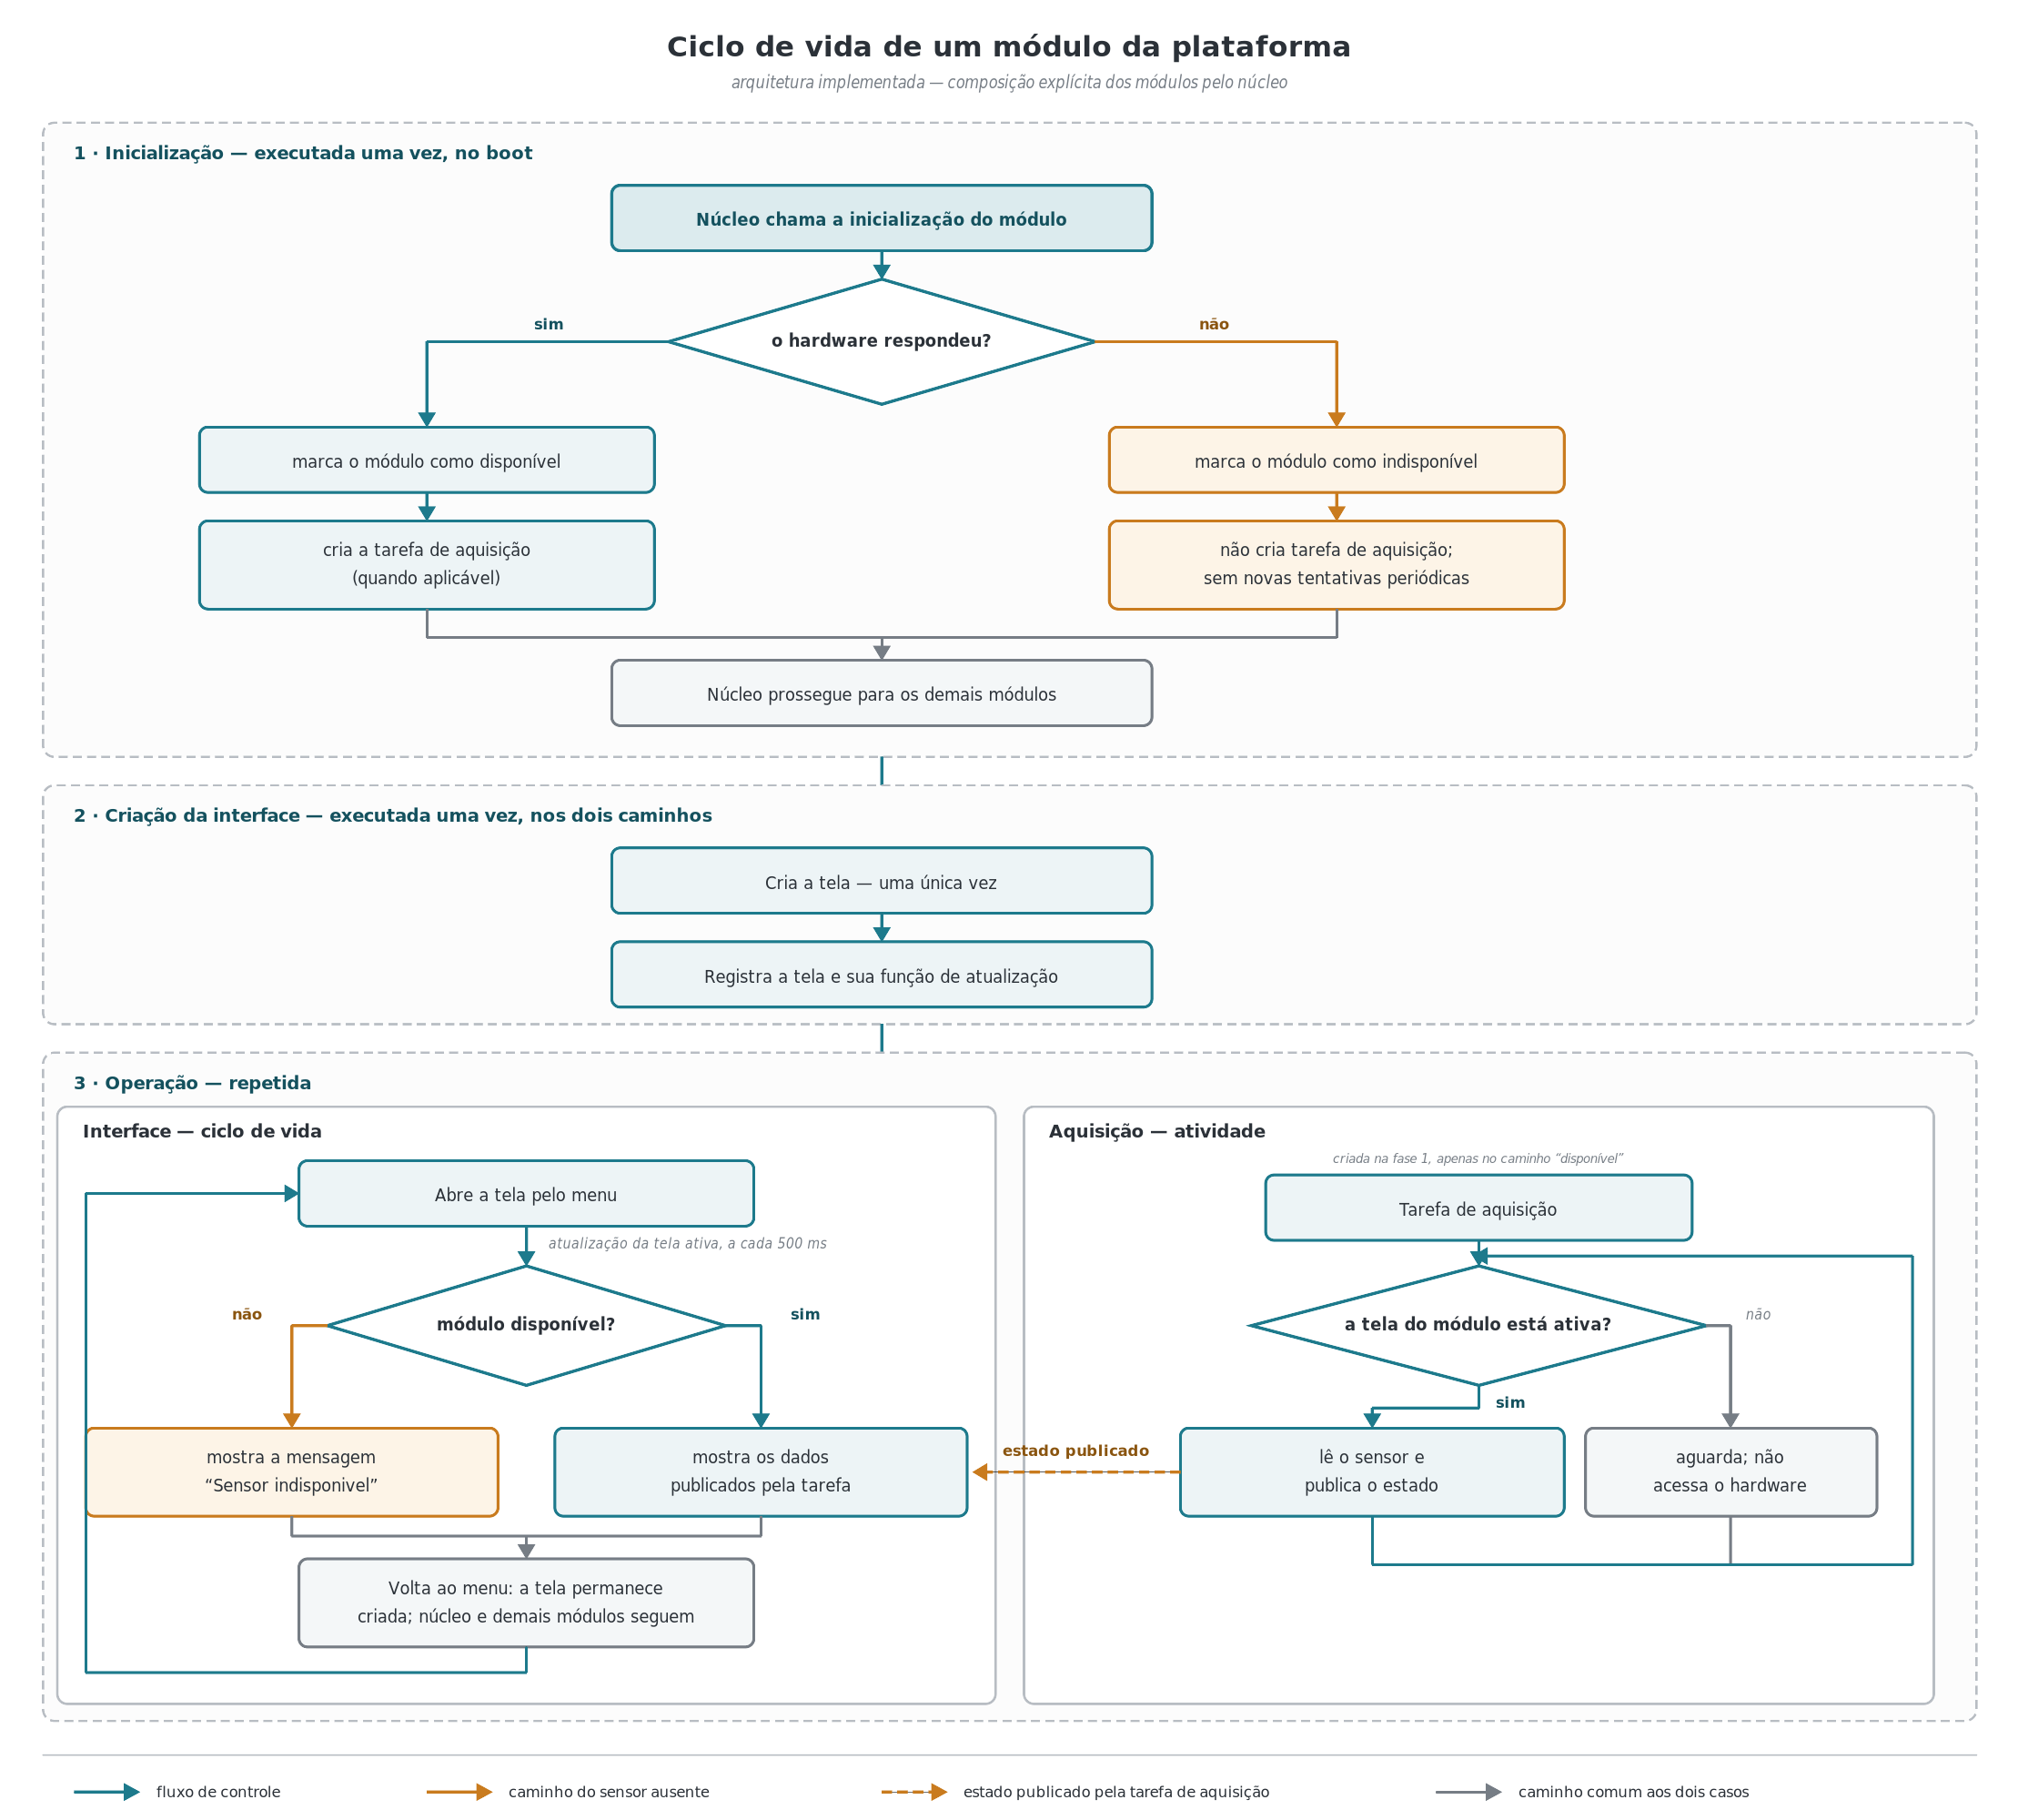
\includegraphics[width=0.94\textwidth]{Diagramas/teoricas/ciclo_vida_modulo.png}
\fonteelemento{Elaborado pelo autor a partir do contrato observado no firmware}
\end{figure}


\subsubsection{Servi\c{c}os do n\'ucleo}


O registro de telas associa um objeto LVGL a uma fun\c{c}\~ao de atualiza\c{c}\~ao. A cada 500 ms, o despachante consulta a tela ativa e chama somente a fun\c{c}\~ao registrada para ela. Menus est\'aticos n\~ao precisam de atualiza\c{c}\~ao peri\'odica, enquanto telas de sensores convertem o estado publicado pelas tarefas em texto, indicadores ou gr\'aficos.


O n\'ucleo tamb\'em concentra a cria\c{c}\~ao do barramento I$^2$C, o scanner de endere\c{c}os, a recupera\c{c}\~ao ap\'os falhas e os estilos compartilhados da interface. O servi\c{c}o \texttt{app\_perf\_read()} fornece uma estimativa explorat\'oria de ociosidade e o heap livre, mas, sem uma s\'erie controlada, esses valores n\~ao foram usados como caracteriza\c{c}\~ao de desempenho.


\subsubsection{Ciclo de vida dos m\'odulos}


Ap\'os a inicializa\c{c}\~ao dos servi\c{c}os b\'asicos, o n\'ucleo percorre os m\'odulos conhecidos. Cada m\'odulo tenta identificar e configurar seu hardware e registra internamente se ficou dispon\'ivel. A cria\c{c}\~ao das telas ocorre mesmo quando um sensor falha, pois a interface precisa apresentar o estado de indisponibilidade sem depender de nova tentativa cont\'inua.


As tarefas s\~ao criadas somente quando necess\'arias ao m\'odulo. Durante a opera\c{c}\~ao, elas alternam entre bloqueio temporizado, aquisi\c{c}\~ao e publica\c{c}\~ao do estado. A tela consome esse estado sem executar diretamente a transa\c{c}\~ao sensorial, evitando que uma atualiza\c{c}\~ao gr\'afica aguarde uma convers\~ao lenta.


Como a composi\c{c}\~ao dos m\'odulos permanece expl\'icita na implementa\c{c}\~ao corrente, a inclus\~ao de um novo sensor exige tanto a prepara\c{c}\~ao do m\'odulo quanto seu registro no n\'ucleo e na interface. A Figura~\ref{fig:integracao-novo-sensor} organiza esse procedimento a partir dos pontos confirmados no firmware.


\begin{figure}[H]
\centering
\caption{Fluxo para integra\c{c}\~ao de um novo sensor ao firmware}
\label{fig:integracao-novo-sensor}
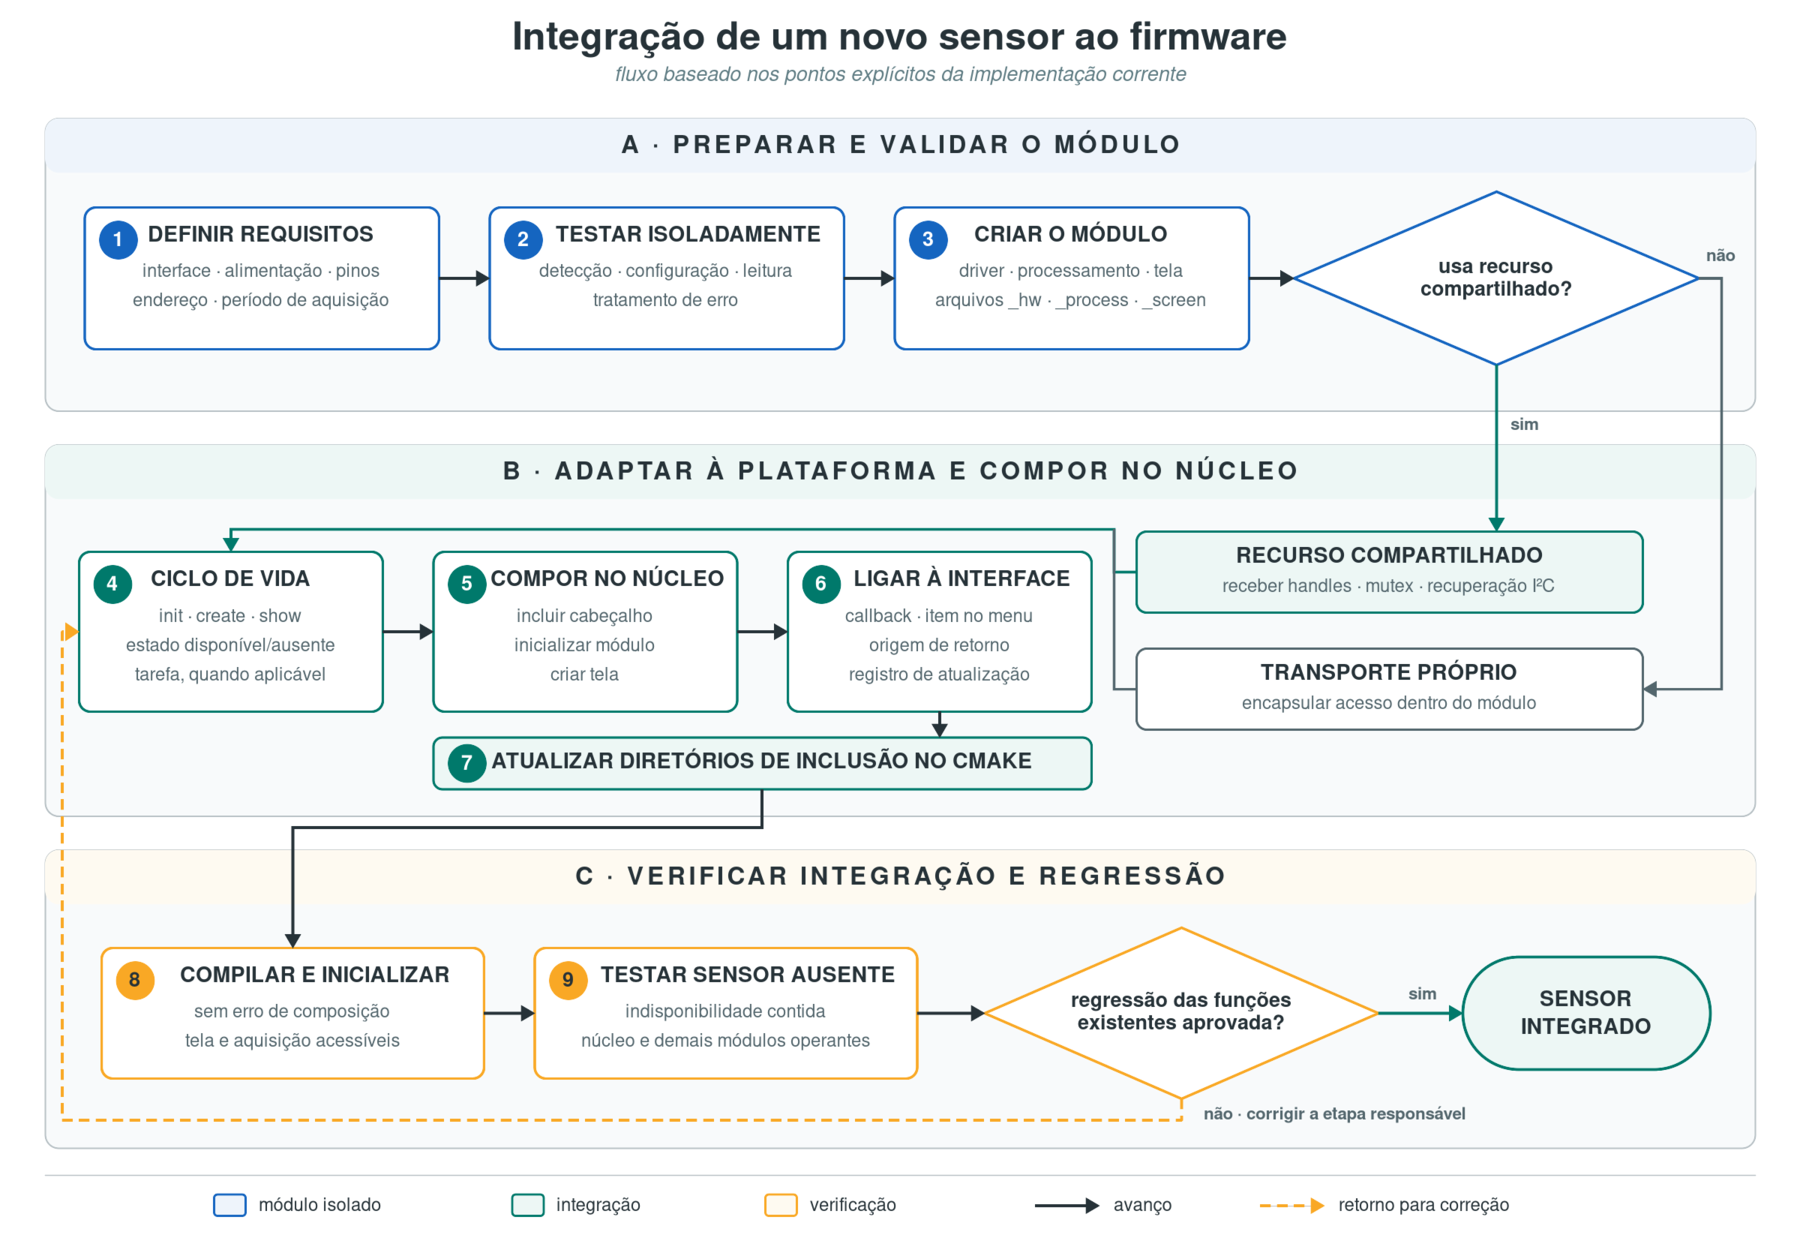
\includegraphics[width=0.95\textwidth]{Diagramas/sistema/integracao_novo_sensor.png}
\fonteelemento{Elaborado pelo autor a partir de \texttt{main.c}, \texttt{app.h}, \texttt{CMakeLists.txt} e da organiza\c{c}\~ao dos m\'odulos sensoriais}
\end{figure}


\subsubsection{Inicializa\c{c}\~ao n\~ao fatal}


A inicializa\c{c}\~ao de um sensor retorna erro ao n\'ucleo, mas esse retorno n\~ao aciona encerramento deliberado da aplica\c{c}\~ao. O m\'odulo marca sua disponibilidade como falsa, preserva uma mensagem apropriada para a tela e n\~ao inicia aquisi\c{c}\~oes que dependam do dispositivo ausente.


O n\'ucleo prossegue com os m\'odulos seguintes e com a cria\c{c}\~ao da interface. Assim, rel\'ogio, toque e sensores presentes podem permanecer dispon\'iveis quando um sensor externo n\~ao responde. A falha de recursos compartilhados, como o pr\'oprio controlador I$^2$C ou o display, possui alcance maior e precisa ser distinguida da aus\^encia isolada de um m\'odulo.


\subsubsection{Modelo de concorr\^encia}


O FreeRTOS opera em configura\c{c}\~ao de n\'ucleo \'unico. A configura\c{c}\~ao padr\~ao usada por \texttt{esp\_lvgl\_port} cria a tarefa gr\'afica com prioridade 4. As tarefas de MAX30102, DS18B20, LTR390, b\'ussola e ped\^ometro s\~ao criadas explicitamente com prioridade 3; a tarefa auxiliar de captura usa prioridade 2; o la\c{c}o de \texttt{app\_main} permanece na tarefa principal do ESP-IDF; e a tarefa ociosa ocupa a prioridade 0.


A frequ\^encia de \emph{tick} foi configurada em 100 Hz, correspondendo a uma resolu\c{c}\~ao de 10 ms. As tarefas aguardam com primitivas de bloqueio e n\~ao realizam espera ocupada entre aquisi\c{c}\~oes. O watchdog de tarefas supervisiona a capacidade de a tarefa ociosa voltar a executar.


As tarefas sensoriais verificam se sua tela est\'a ativa antes de acessar o hardware. Quando a fun\c{c}\~ao n\~ao est\'a em uso, elas bloqueiam por um intervalo e voltam a verificar o estado. Esse condicionamento reduz transa\c{c}\~oes e processamento sem suspender ou destruir repetidamente as tarefas.


A Figura~\ref{fig:tarefas-freertos} organiza as tarefas confirmadas, suas prioridades e os recursos compartilhados.


\begin{figure}[H]
\centering
\caption{Tarefas FreeRTOS e recursos compartilhados no n\'ucleo \'unico}
\label{fig:tarefas-freertos}
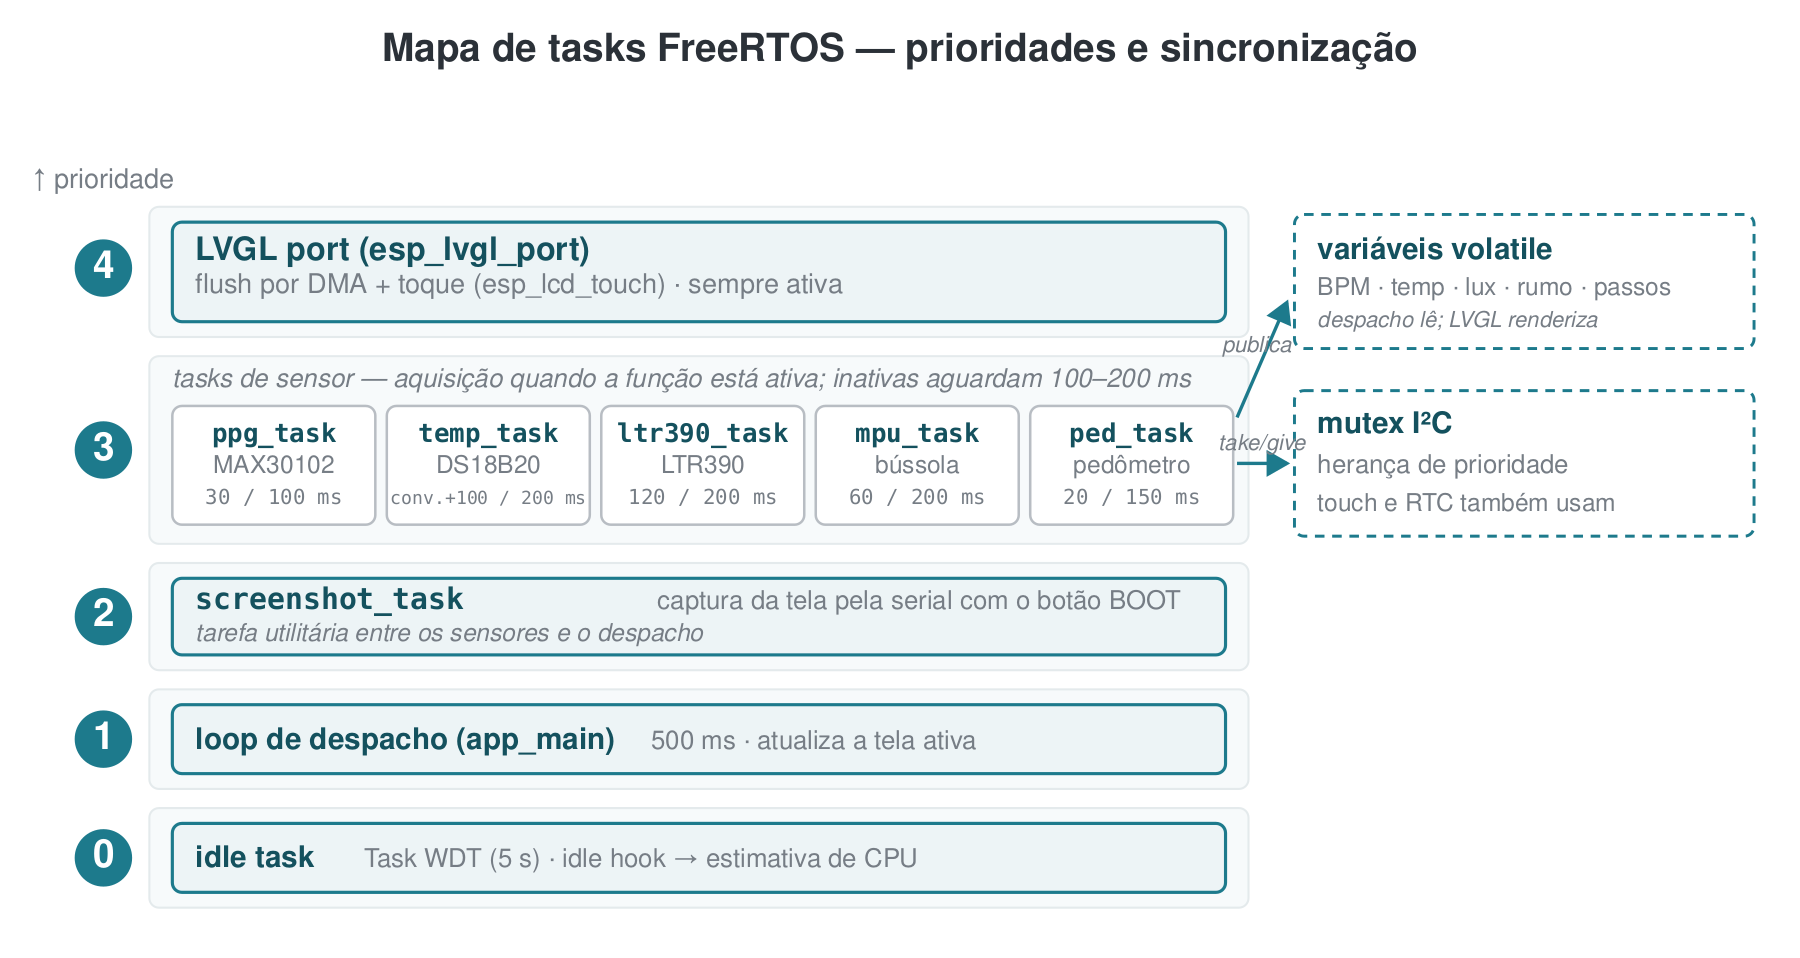
\includegraphics[width=0.98\textwidth]{Diagramas/sistema/freertos_tasks.png}
\fonteelemento{Elaborado pelo autor a partir do firmware e da configura\c{c}\~ao do ESP-IDF}
\end{figure}


\subsubsection{Comunica\c{c}\~ao entre tarefas e interface}


As tarefas publicam as \'ultimas medidas v\'alidas e indicadores de estado em vari\'aveis pertencentes ao m\'odulo. A fun\c{c}\~ao de atualiza\c{c}\~ao da tela l\^e uma fotografia desses valores sob a prote\c{c}\~ao adequada ao tipo de dado. Vari\'aveis escalares alinhadas de at\'e 32 bits podem ser lidas atomicamente pelo processador, mas conjuntos de valores correlacionados exigem cuidado para que a tela n\~ao combine amostras de instantes diferentes.


Apenas o contexto autorizado pela porta da LVGL altera objetos gr\'aficos. Quando uma fun\c{c}\~ao externa ao contexto gr\'afico precisa atualizar a interface, ela obt\'em o bloqueio fornecido pela integra\c{c}\~ao do LVGL. A aquisi\c{c}\~ao permanece independente desse bloqueio para n\~ao reter o recurso gr\'afico durante transa\c{c}\~oes ou processamento.


\subsubsection{Inclus\~ao de novo m\'odulo}


A inclus\~ao de uma nova fun\c{c}\~ao segue uma sequ\^encia definida: implementar ou selecionar o driver; criar o estado e a tarefa, quando necess\'arios; implementar as tr\^es opera\c{c}\~oes do ciclo de vida; registrar a tela e sua atualiza\c{c}\~ao; adicionar o acesso \`a navega\c{c}\~ao. Servi\c{c}os novos somente devem ser acrescentados ao n\'ucleo se forem compartilhados por mais de um m\'odulo ou representarem uma responsabilidade global.


Esse procedimento descreve o ponto de extens\~ao implementado, mas n\~ao quantifica seu custo. O n\'umero de arquivos alterados, as mudan\c{c}as no n\'ucleo e o efeito sobre m\'odulos existentes ser\~ao determinados pelo ensaio de extensibilidade.


\subsection{Robustez do barramento I$^2$C}


\subsubsection{Problema do NACK}


Durante a integra\c{c}\~ao, um NACK deixou de ser apenas um erro local de leitura. Como os dispositivos compartilham controlador e linhas, uma transa\c{c}\~ao interrompida podia afetar a opera\c{c}\~ao seguinte, ainda que destinada a outro endere\c{c}o. Os documentos de desenvolvimento registram ocorr\^encias em que o controlador retornou estado inv\'alido depois da falha inicial.


Cada driver passou a tratar o retorno da API em todas as transa\c{c}\~oes. A aus\^encia de ACK n\~ao \'e interpretada como dado nulo nem ignorada. O m\'odulo recebe o erro, evita publicar uma amostra inv\'alida e aciona o procedimento comum de recupera\c{c}\~ao antes de uma tentativa posterior.


\subsubsection{Mutex com heran\c{c}a de prioridade}


Um mutex \'unico protege as transa\c{c}\~oes do barramento. A tarefa o obt\'em antes da sequ\^encia que deve permanecer indivis\'ivel, executa o acesso e o libera em todos os caminhos de sa\'ida. A prote\c{c}\~ao abrange a transa\c{c}\~ao completa, incluindo sele\c{c}\~ao de registrador e leitura subsequente quando essas etapas formam uma opera\c{c}\~ao l\'ogica.


Foi utilizado mutex, e n\~ao sem\'aforo bin\'ario, para dispor da heran\c{c}a de prioridade oferecida pelo FreeRTOS. Se uma tarefa priorit\'aria aguarda o barramento retido por outra de menor prioridade, a tarefa propriet\'aria pode herdar temporariamente a prioridade at\'e concluir a regi\~ao protegida.


\subsubsection{Recupera\c{c}\~ao do barramento}


O servi\c{c}o de recupera\c{c}\~ao encapsula a chamada \texttt{i2c\_master\_bus\_reset()} oferecida pela API mestre do ESP-IDF (ESPRESSIF SYSTEMS, 2025g). Quando uma transa\c{c}\~ao falha, o driver solicita a recupera\c{c}\~ao ainda dentro do fluxo controlado e somente depois libera o mutex. Dessa forma, outra tarefa n\~ao inicia uma transa\c{c}\~ao enquanto o controlador permanece no estado associado \`a falha anterior.


O reset n\~ao garante que um dispositivo ausente volte a responder. Sua finalidade \'e devolver o controlador e as linhas a uma condi\c{c}\~ao na qual os demais dispositivos possam ser acessados. O n\'umero de tentativas permanece limitado para evitar um ciclo indefinido de falha e recupera\c{c}\~ao.


A ordem do caminho normal e da recupera\c{c}\~ao p\'os-NACK \'e apresentada na Figura~\ref{fig:i2c-recuperacao}.


\begin{figure}[H]
\centering
\caption{Transa\c{c}\~ao I$^2$C e recupera\c{c}\~ao ap\'os falha}
\label{fig:i2c-recuperacao}
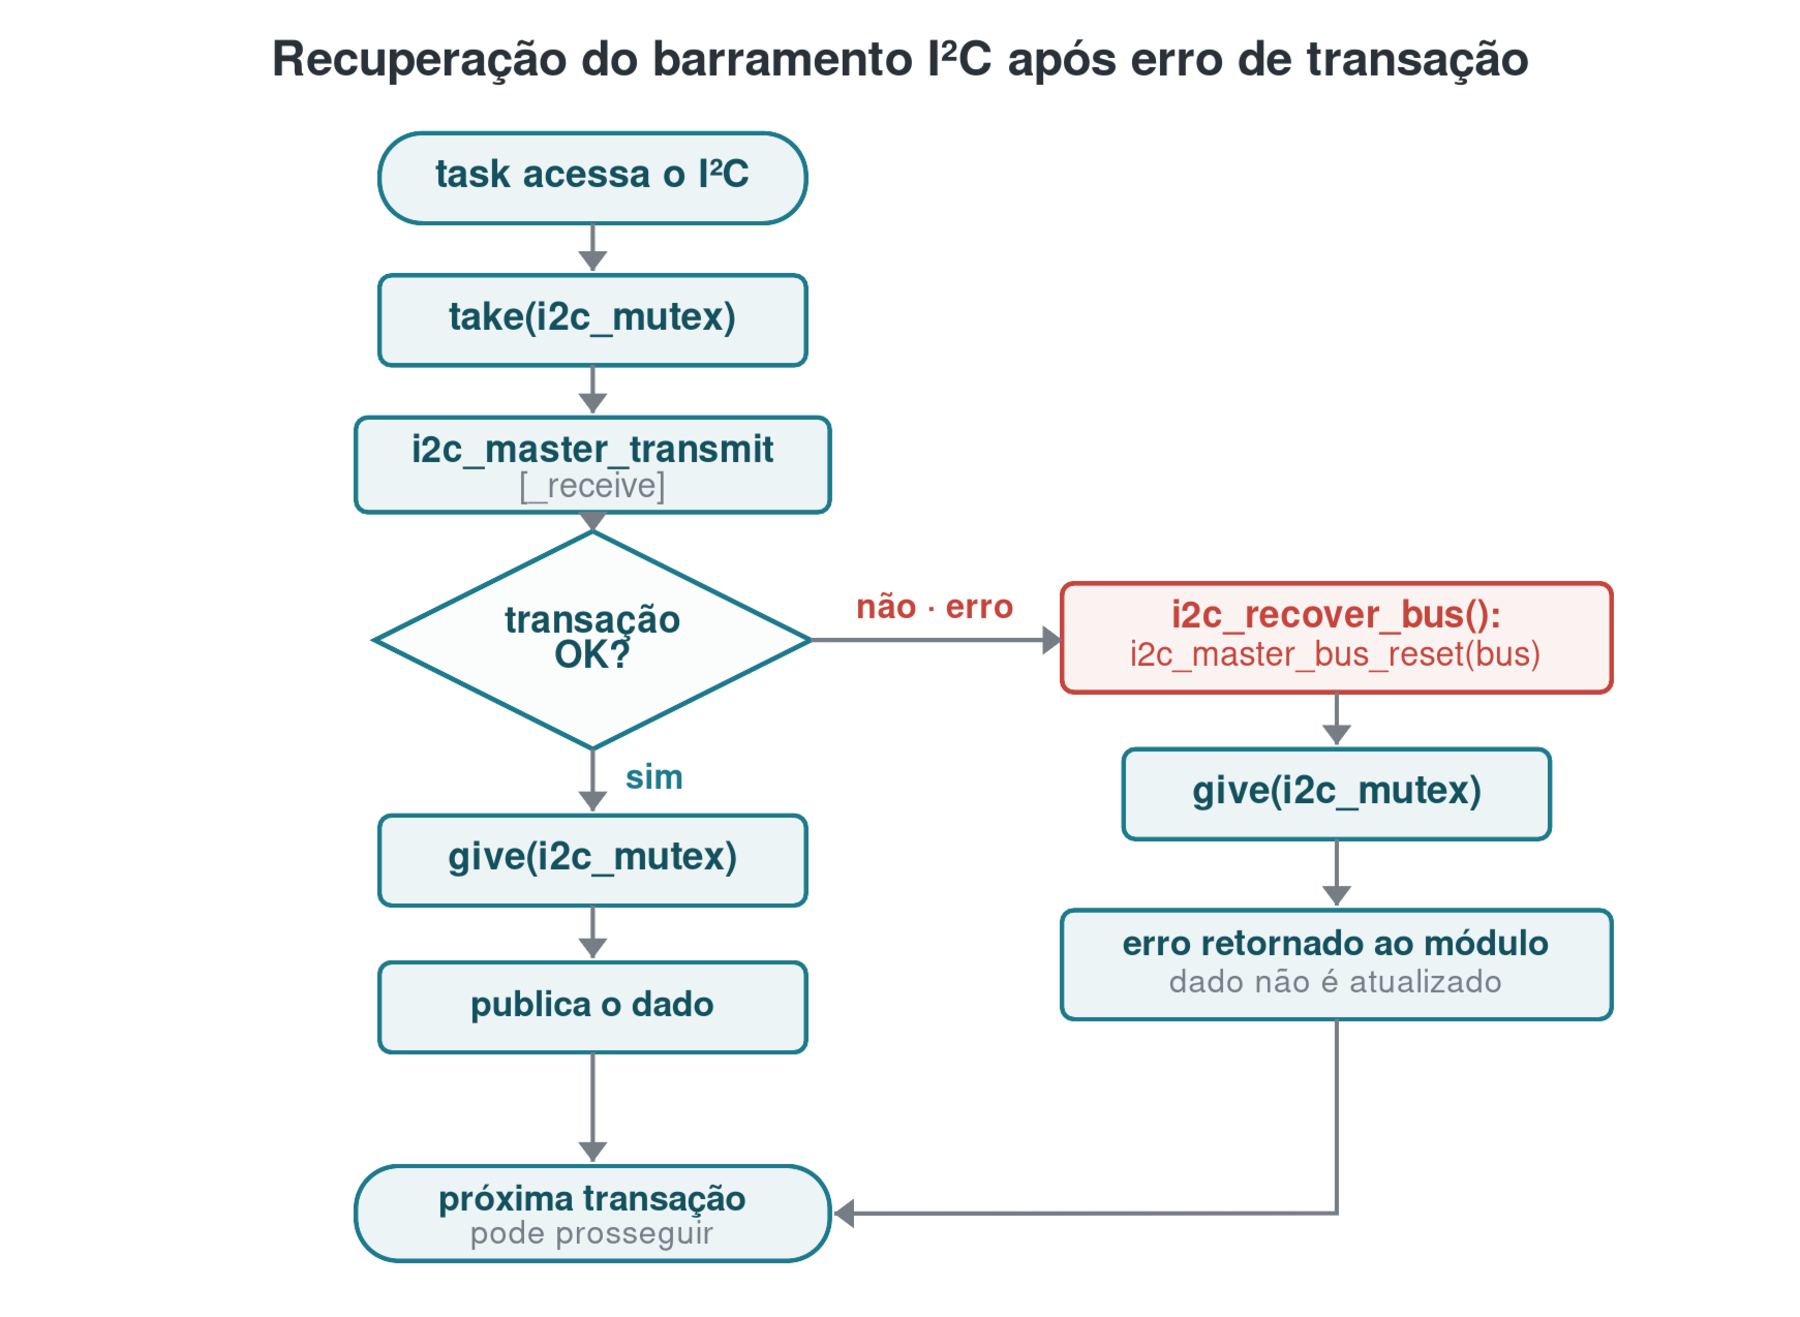
\includegraphics[width=0.94\textwidth]{Diagramas/sistema/i2c_recuperacao_nack.png}
\fonteelemento{Elaborado pelo autor a partir de \texttt{i2c\_recover.c} e dos drivers integrados}
\end{figure}


\subsubsection{Scanner no boot}


Ap\'os criar o barramento, o firmware percorre os endere\c{c}os poss\'iveis e registra os dispositivos que respondem. O scanner foi usado como diagn\'ostico da montagem e permitiu distinguir endere\c{c}o incorreto, sensor ausente e problema geral das linhas.


O resultado da varredura n\~ao substitui a inicializa\c{c}\~ao dos drivers. Responder ao endere\c{c}o demonstra presen\c{c}a no barramento, mas n\~ao confirma identidade, configura\c{c}\~ao nem validade dos dados.


\subsubsection{Redu\c{c}\~ao das transa\c{c}\~oes do touch}


O controlador CHSC6X fornece um sinal de interrup\c{c}\~ao associado ao toque. A primeira integra\c{c}\~ao consultava o dispositivo por I$^2$C mesmo quando n\~ao havia intera\c{c}\~ao. O driver foi alterado para verificar o GPIO17 e iniciar a leitura somente quando o sinal indica evento ativo.


Essa decis\~ao reduz o uso do barramento por uma fun\c{c}\~ao que, na maior parte do tempo, permanece ociosa. A quantifica\c{c}\~ao da redu\c{c}\~ao pertence aos resultados; no desenvolvimento, o aspecto relevante \'e que a interface passou a utilizar uma indica\c{c}\~ao f\'isica de disponibilidade antes da transa\c{c}\~ao.


\subsubsection{Efeito dos logs no sistema}


Mensagens repetidas do driver I$^2$C durante uma sequ\^encia de erros aumentavam o trabalho de formata\c{c}\~ao e transmiss\~ao serial. Em um sistema de n\'ucleo \'unico, essa atividade concorria com a interface e com tarefas temporizadas. Os n\'iveis de log dos componentes mais verbosos foram reduzidos na opera\c{c}\~ao normal, preservando mensagens resumidas e contadores de falha.


Logs detalhados continuam \'uteis em vers\~oes de diagn\'ostico. Sua ativa\c{c}\~ao deve ser tratada como instrumenta\c{c}\~ao capaz de alterar o comportamento temporal, especialmente durante ensaios de CPU, boot e estabilidade.


\subsection{Interface gr\'afica e rel\'ogio}


\subsubsection{Inicializa\c{c}\~ao do display}


O SPI2 \'e configurado antes da cria\c{c}\~ao da interface gr\'afica. O componente do GC9A01A recebe os GPIOs, a frequ\^encia de 40 MHz, a resolu\c{c}\~ao e os par\^ametros de transforma\c{c}\~ao do painel. Ap\'os a sequ\^encia de inicializa\c{c}\~ao, a porta do LVGL associa o buffer de desenho \`a fun\c{c}\~ao de transfer\^encia do controlador.


O conte\'udo foi limitado a uma regi\~ao \'util menor que o ret\^angulo de 240 $\times$ 240 pixels, evitando cortar textos e controles pr\'oximos aos cantos invis\'iveis do painel circular.


\subsubsection{Integra\c{c}\~ao com LVGL}


O \texttt{esp\_lvgl\_port} coordena o temporizador da biblioteca, a entrada por toque e a transfer\^encia das regi\~oes invalidadas. As telas foram constru\'idas com widgets, estilos e fontes, em vez de imagens de quadro completo. Essa estrat\'egia permite alterar valores e indicadores sem armazenar uma imagem integral para cada m\'odulo.


Cada tela \'e criada uma vez e mantida para reutiliza\c{c}\~ao. A navega\c{c}\~ao troca o objeto exibido, enquanto o registro do n\'ucleo seleciona a rotina de atualiza\c{c}\~ao apropriada. Opera\c{c}\~oes que modificam objetos utilizam o bloqueio da porta gr\'afica.


\subsubsection{Corre\c{c}\~ao de cores}


A representa\c{c}\~ao RGB565 exigiu alinhar a ordem dos bytes produzidos pelo LVGL, a ordem dos elementos de cor e a invers\~ao configurada no painel. A configura\c{c}\~ao consolidada combina troca dos bytes de 16 bits, ordem BGR e invers\~ao de cor do controlador.


Esses par\^ametros atuam em n\'iveis diferentes e n\~ao devem ser atribu\'idos somente ao \emph{endianness} do processador. No firmware corrente, \texttt{main.c} define ordem BGR e invers\~ao no controlador, enquanto a op\c{c}\~ao de troca de bytes do RGB565 permanece na configura\c{c}\~ao da LVGL.


\subsubsection{Navega\c{c}\~ao}


A interface utiliza quatro p\'aginas de menu na ordem execut\'avel: sinais vitais, com cora\c{c}\~ao e temperatura; luz e UV; movimento, com b\'ussola e ped\^ometro; e configura\c{c}\~oes de hora e data. A tela principal abre a primeira p\'agina, e as setas laterais percorrem as quatro p\'aginas em sequ\^encia.


A navega\c{c}\~ao \'e independente dos detalhes do sensor. O item conhece a fun\c{c}\~ao p\'ublica usada para exibir a tela, mas n\~ao acessa dados, registradores nem tarefas do m\'odulo.


A Figura~\ref{fig:mapa-navegacao} apresenta os acessos aos m\'odulos, os caminhos de retorno e as telas auxiliares.


\begin{figure}[H]
\centering
\caption{Mapa de navega\c{c}\~ao da interface do prot\'otipo}
\label{fig:mapa-navegacao}
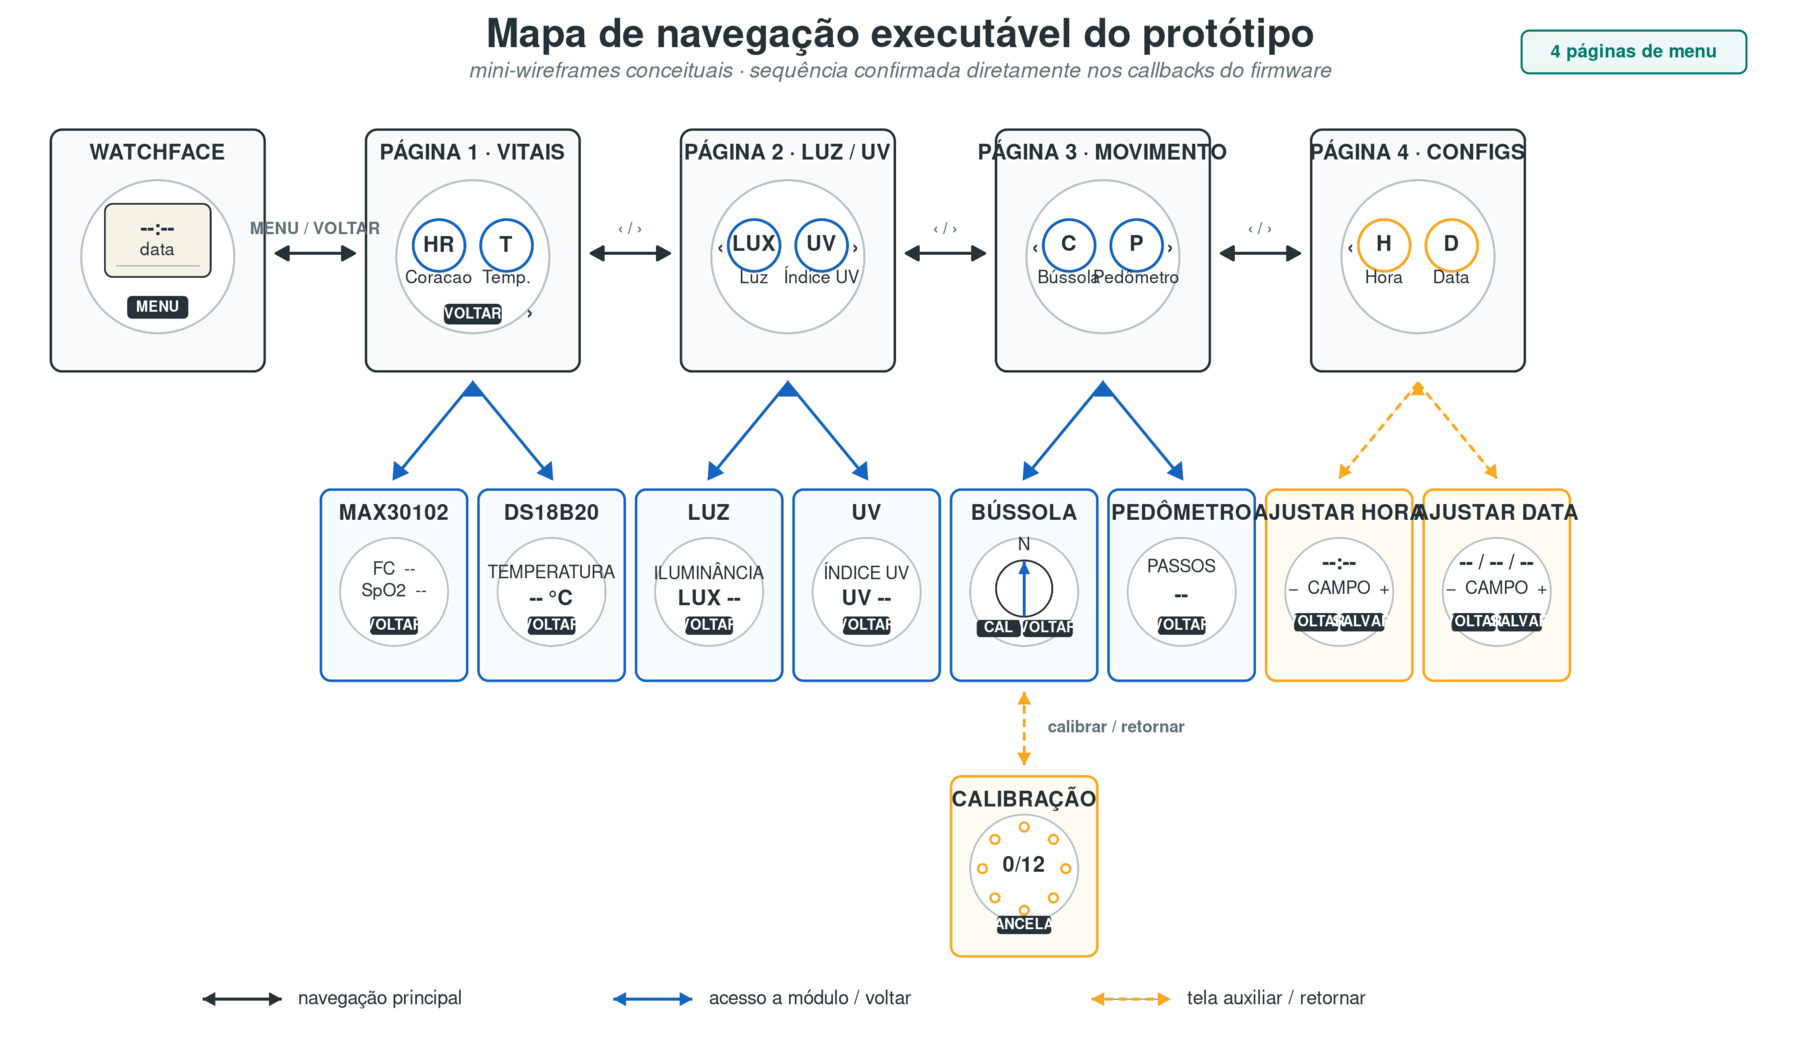
\includegraphics[width=0.98\textwidth]{Diagramas/teoricas/mapa_navegacao.png}
\fonteelemento{Elaborado pelo autor a partir dos \emph{callbacks} e arquivos de tela do firmware}
\end{figure}


\subsubsection{Tela principal}


A tela principal apresenta hora e data obtidas do PCF8563. Um anel de 60 marcadores distribui a indica\c{c}\~ao dos segundos ao redor da circunfer\^encia. Os elementos centrais permanecem dentro do raio \'util e s\~ao atualizados sem reconstruir a tela inteira.


O rel\'ogio tamb\'em oferece o ponto de entrada para a configura\c{c}\~ao de data e hora. A atualiza\c{c}\~ao peri\'odica l\^e os campos necess\'arios do RTC e converte sua representa\c{c}\~ao antes de alterar os r\'otulos.


\subsubsection{Fonte otimizada}


A fonte monoespa\c{c}ada usada na hora foi gerada somente com os algarismos de zero a nove e o caractere de dois-pontos, totalizando 11 glifos. A redu\c{c}\~ao evita incorporar caracteres que n\~ao aparecem naquele r\'otulo.


Como a fonte n\~ao cont\'em espa\c{c}o, o campo ativo na edi\c{c}\~ao n\~ao pode ser ocultado por substitui\c{c}\~ao textual. O firmware varia a opacidade do objeto, mantendo a indica\c{c}\~ao visual sem ampliar o conjunto de glifos.


\subsubsection{Configura\c{c}\~ao por toque}


Dois controles na tela permitem avan\c{c}ar o valor atual e confirmar a etapa. Uma m\'aquina de estados percorre hora, minuto, dia, m\^es e ano. Ao confirmar o \'ultimo campo, o firmware determina o dia da semana e grava o conjunto no PCF8563.


Durante a edi\c{c}\~ao, o campo ativo alterna sua opacidade para indicar qual valor ser\'a alterado. A implementa\c{c}\~ao n\~ao depende de bot\~oes f\'isicos externos ao Round Display.


\subsubsection{RTC PCF8563}


O driver pr\'oprio l\^e sete bytes consecutivos a partir do registrador de segundos. Os valores armazenados em BCD s\~ao convertidos para inteiros e reunidos em uma estrutura de data e hora. Na escrita, o caminho inverso prepara os campos e preserva os bits de controle definidos pelo dispositivo.


O dia da semana \'e calculado a partir da data informada antes da grava\c{c}\~ao. A bateria de reserva do Round Display mant\'em o RTC durante a interrup\c{c}\~ao da alimenta\c{c}\~ao principal. O RTC n\~ao participa da recupera\c{c}\~ao de tempo por rede, pois sincroniza\c{c}\~ao por NTP n\~ao foi implementada.


\subsection{M\'odulo MAX30102}


\subsubsection{Configura\c{c}\~ao}


O driver verifica a identidade do MAX30102 e programa o modo de aquisi\c{c}\~ao dos canais vermelho e infravermelho. A configura\c{c}\~ao corrente utiliza taxa de 100 amostras por segundo, resolu\c{c}\~ao de 18 bits, faixa do conversor de 16.384 nA e corrente aproximada de 7,2 mA em cada emissor. Esses valores correspondem, respectivamente, a 0x67 em \texttt{SPO2\_CONFIG} e 0x24 nos registradores de corrente dos LED.


O componente permanece em \emph{shutdown} quando n\~ao h\'a medi\c{c}\~ao solicitada. A tela oferece um comando de in\'icio, evitando manter os emissores ativos continuamente.


\subsubsection{FIFO e aquisi\c{c}\~ao}


A FIFO desacopla a produ\c{c}\~ao das amostras do instante exato em que a tarefa obt\'em o barramento. A tarefa consulta a quantidade dispon\'ivel, l\^e os bytes em bloco e recomp\~oe cada valor de 18 bits. Os ponteiros da FIFO e condi\c{c}\~oes de transbordamento s\~ao verificados para evitar processar dados incompletos como amostras v\'alidas.


Cada amostra \'e encaminhada ao detector de contato e, quando aceita, \`as etapas de condicionamento. A interface consome apenas os valores publicados pelo processamento, sem drenar a FIFO no contexto gr\'afico.


O fluxo completo, incluindo as portas de aceita\c{c}\~ao que podem rejeitar uma amostra ou um pulso, \'e sintetizado na Figura~\ref{fig:max30102-fluxo}.


\begin{figure}[H]
\centering
\caption{Aquisi\c{c}\~ao e processamento implementados no m\'odulo MAX30102}
\label{fig:max30102-fluxo}
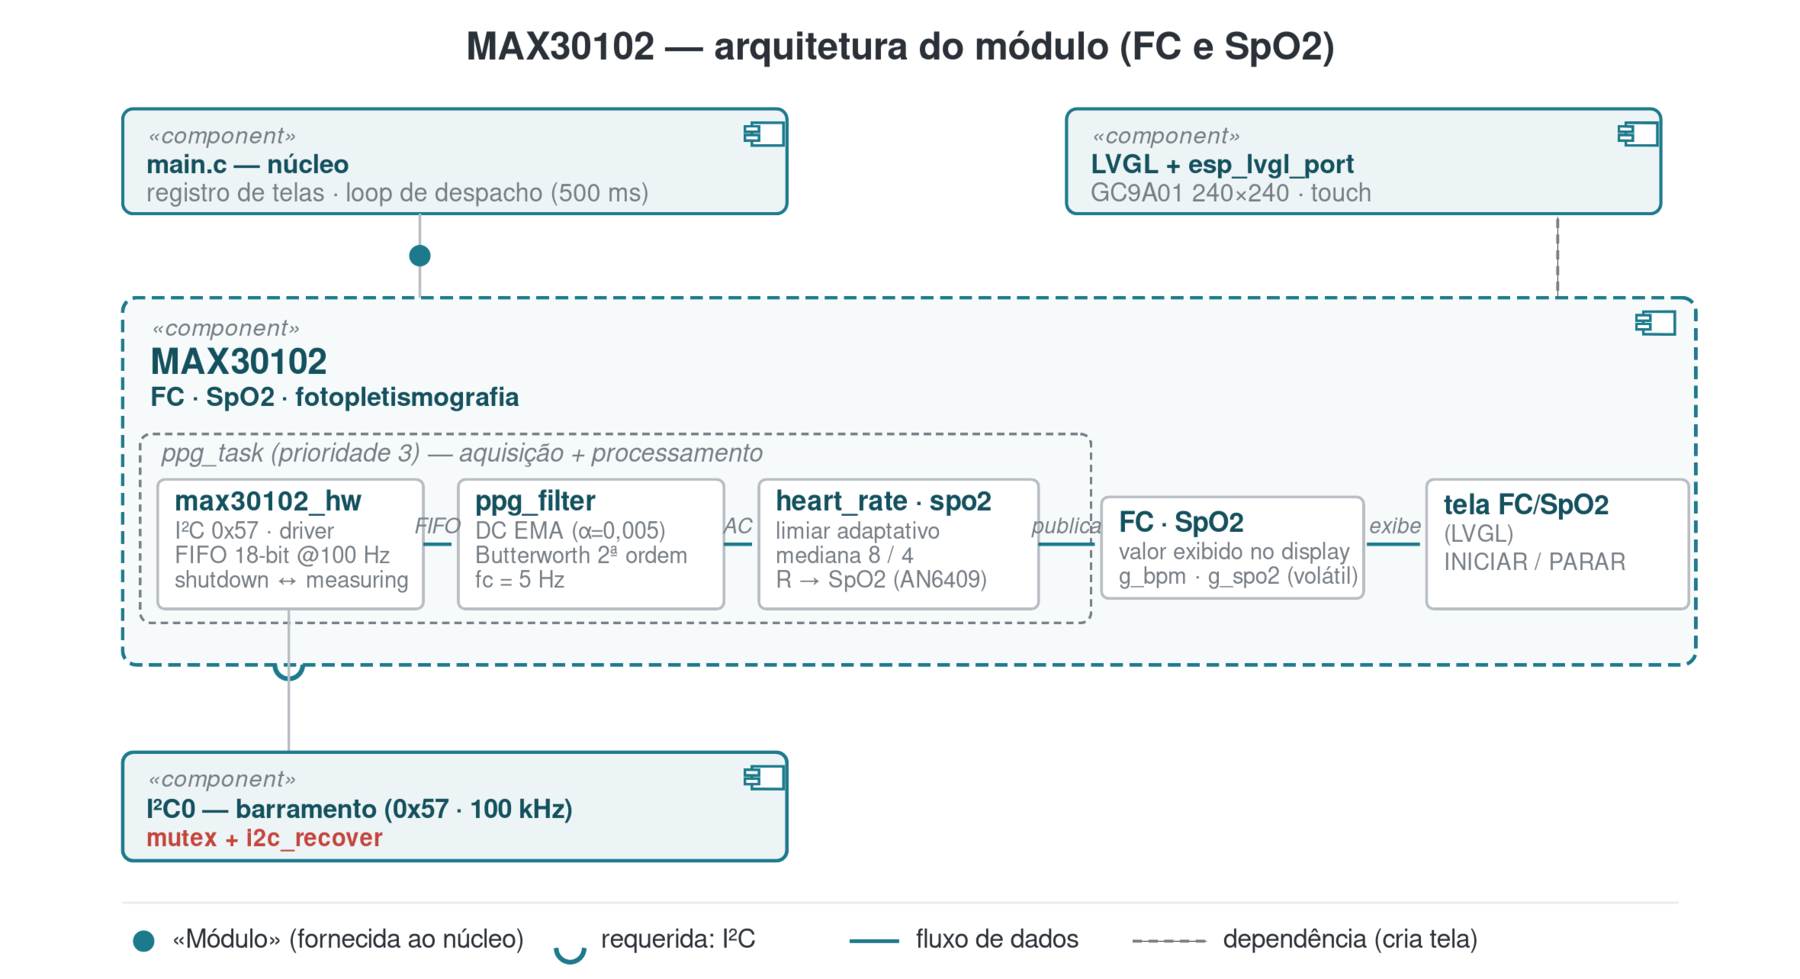
\includegraphics[width=0.96\textwidth]{Diagramas/max30102/max30102_modulo.png}
\fonteelemento{Elaborado pelo autor a partir de \texttt{max30102\_hw.c}, \texttt{ppg\_filter.c}, \texttt{heart\_rate.c} e \texttt{spo2.c}}
\end{figure}


\subsubsection{Detec\c{c}\~ao de dedo}


A presen\c{c}a de contato \'e inferida do n\'ivel do sinal \'optico bruto com limiares distintos para entrada e sa\'ida. A histerese reduz altern\^ancias quando o valor permanece pr\'oximo ao limite. Ao perder contato, o m\'odulo invalida as estimativas e reinicializa estados que n\~ao devem atravessar duas aquisi\c{c}\~oes independentes.


Essa detec\c{c}\~ao indica somente que o n\'ivel \'optico \'e compat\'ivel com contato. Ela n\~ao garante qualidade suficiente para estimar frequ\^encia card\'iaca ou SpO$_2$.


\subsubsection{Filtragem}


Uma m\'edia m\'ovel exponencial acompanha a componente DC. Durante as primeiras 300 amostras, o coeficiente \'e 0,1 para acelerar a estabiliza\c{c}\~ao; depois, passa a $\alpha=0{,}005$. A subtra\c{c}\~ao produz a componente puls\'atil, que passa por um filtro Butterworth de segunda ordem com frequ\^encia de corte de 5 Hz. A frequ\^encia de amostragem usada no c\'alculo dos coeficientes \'e 100 Hz.


Os estados dos filtros s\~ao preservados entre amostras consecutivas e reiniciados quando come\c{c}a uma nova sess\~ao ou quando o contato \'e perdido. O detector ignora as primeiras 500 amostras de cada sess\~ao para que os transientes dos dois est\'agios decaiam antes de publicar batimentos.


\subsubsection{Frequ\^encia card\'iaca}


A detec\c{c}\~ao utiliza uma diferen\c{c}a com intervalo de quatro amostras, o cruzamento de sua derivada associado a um m\'aximo e um limiar adaptativo de amplitude. Candidatos abaixo de 30\% do limiar corrente ou com amplitude absoluta inferior ao limite implementado s\~ao rejeitados. Um per\'iodo refrat\'ario de 400 ms impede que oscila\c{c}\~oes pr\'oximas sejam interpretadas como batimentos distintos.


A frequ\^encia card\'iaca \'e calculada a partir dos intervalos entre batimentos. Uma mediana sobre oito intervalos reduz a influ\^encia de uma detec\c{c}\~ao isolada. Quando n\~ao h\'a quantidade suficiente de eventos v\'alidos, a tela mant\'em a estimativa como indispon\'ivel.


\subsubsection{Estimativa de SpO$_2$}


Para cada batimento aceito, o m\'odulo obt\'em componentes AC e DC dos canais vermelho e infravermelho e calcula a raz\~ao de raz\~oes. A convers\~ao consolidada utiliza a rela\c{c}\~ao emp\'irica


\[
\widehat{\mathrm{SpO_2}}=-45{,}060R^2+30{,}354R+94{,}845.
\]


Crit\'erios de qualidade rejeitam denominadores inadequados, raz\~oes fora da faixa admitida e pulsos com baixa modula\c{c}\~ao. A sa\'ida \'e suavizada pela mediana de quatro estimativas aceitas. O valor permanece denominado estimativa de SpO$_2$, pois a implementa\c{c}\~ao n\~ao passou por valida\c{c}\~ao cl\'inica.


\subsubsection{Invers\~ao dos canais em placas de conex\~ao}


Durante a depura\c{c}\~ao, a ordem observada dos canais em determinadas placas de conex\~ao n\~ao correspondeu \`a atribui\c{c}\~ao inicialmente presumida. Os tr\^es primeiros bytes de cada amostra foram tratados como infravermelho e os tr\^es seguintes como vermelho na montagem utilizada.


Essa corre\c{c}\~ao pertence \`a associa\c{c}\~ao entre o componente e a placa espec\'ifica, n\~ao a uma invers\~ao universal do MAX30102. O driver deve registrar ou encapsular a ordem adotada para impedir que o processamento receba canais trocados.


\subsubsection{Integra\c{c}\~ao com tarefa e tela}


A tarefa do m\'odulo permanece bloqueada quando a tela n\~ao est\'a ativa ou quando a medi\c{c}\~ao n\~ao foi iniciada. Durante uma sess\~ao, ela obt\'em o mutex, drena a FIFO, libera o barramento e executa o processamento. A tela apresenta estado de contato, frequ\^encia card\'iaca e estimativa de SpO$_2$.


Falhas de comunica\c{c}\~ao invalidam a aquisi\c{c}\~ao corrente e acionam a recupera\c{c}\~ao comum do I$^2$C. A interface continua naveg\'avel e diferencia sensor indispon\'ivel, aus\^encia de contato e estimativa ainda n\~ao estabilizada.


\subsection{M\'odulo DS18B20}


\subsubsection{Componente oficial e RMT}


O m\'odulo utiliza os componentes oficiais do barramento 1-Wire e do DS18B20. A cria\c{c}\~ao do barramento informa o GPIO20 e seleciona o RMT como mecanismo de temporiza\c{c}\~ao. O sensor encontrado \'e associado ao componente de n\'ivel superior, que oferece opera\c{c}\~oes de configura\c{c}\~ao e leitura.


Essa reutiliza\c{c}\~ao evita manter no projeto uma segunda implementa\c{c}\~ao dos intervalos do protocolo e da verifica\c{c}\~ao CRC. O m\'odulo permanece respons\'avel pelo ciclo funcional e pela apresenta\c{c}\~ao.


\subsubsection{Ciclo de convers\~ao}


O sensor foi configurado para 11 bits. A tarefa solicita uma convers\~ao, bloqueia durante 375 ms e depois l\^e o \emph{scratchpad}. Esse tempo corresponde \`a resolu\c{c}\~ao selecionada na chamada efetiva de configura\c{c}\~ao.


A espera ocorre por bloqueio da tarefa, e n\~ao por la\c{c}o ativo. Como a temperatura varia lentamente, uma nova convers\~ao s\'o \'e solicitada no per\'iodo definido pelo m\'odulo e quando sua fun\c{c}\~ao est\'a ativa.


\subsubsection{CRC e formata\c{c}\~ao}


O componente verifica o CRC antes de entregar a temperatura. Leituras com erro ou fora da faixa funcional definida para a aplica\c{c}\~ao n\~ao substituem a \'ultima amostra v\'alida. O processamento aplica uma m\'edia m\'ovel exponencial com $\alpha=0{,}5$ e a tela apresenta o resultado com uma casa decimal.


A configura\c{c}\~ao do LVGL adotada n\~ao oferece formata\c{c}\~ao direta de ponto flutuante pela fun\c{c}\~ao usada nos r\'otulos. O m\'odulo converte o valor para d\'ecimos de grau e separa sinal, parte inteira e parte decimal antes de construir o texto.


\subsubsection{Integra\c{c}\~ao com tarefa e tela}


A inicializa\c{c}\~ao do DS18B20 n\~ao recebe o barramento nem o mutex I$^2$C. Depois de encontrar e configurar o sensor, o m\'odulo cria sua tarefa e publica temperatura e estado. A tela l\^e esses dados e apresenta indisponibilidade quando a inicializa\c{c}\~ao ou a leitura falha.


\subsection{M\'odulo LTR390}


\subsubsection{Configura\c{c}\~ao}


O driver adiciona o LTR390 ao barramento no endere\c{c}o 0x53 e a 100 kHz, verifica sua identifica\c{c}\~ao e programa resolu\c{c}\~ao de 18 bits com integra\c{c}\~ao e taxa de 100 ms. A configura\c{c}\~ao associa ganho 3$\times$ ao canal de luz ambiente e ganho 18$\times$ ao canal ultravioleta.


\subsubsection{ALS e UVS}


Os canais ALS e UVS utilizam o mesmo conversor e n\~ao operam simultaneamente. O estado do m\'odulo registra o modo configurado, a disponibilidade de nova amostra e as m\'edias mantidas separadamente para ilumin\^ancia e UVI.


Uma solicita\c{c}\~ao da tela de luz seleciona ALS, enquanto a tela de ultravioleta seleciona UVS. Essa decis\~ao permanece interna ao m\'odulo e n\~ao modifica o n\'ucleo nem o driver de outro sensor.


\subsubsection{Altern\^ancia e estabiliza\c{c}\~ao}


Quando o modo solicitado difere do atual, o driver reconfigura o sensor e o m\'odulo descarta as tr\^es primeiras amostras. O descarte impede que valores produzidos durante a transi\c{c}\~ao sejam publicados como pertencentes ao novo canal.


A tarefa s\'o alterna quando a fun\c{c}\~ao ativa exige outro modo. N\~ao h\'a comuta\c{c}\~ao cont\'inua em segundo plano para manter simultaneamente dois valores que n\~ao est\~ao sendo exibidos.


A Figura~\ref{fig:ltr390-estados} explicita que o modo segue a tela ativa e que os valores somente se tornam v\'alidos para a interface ap\'os o descarte das tr\^es amostras.


\begin{figure}[H]
\centering
\caption{M\'aquina de estados implementada para o LTR390}
\label{fig:ltr390-estados}
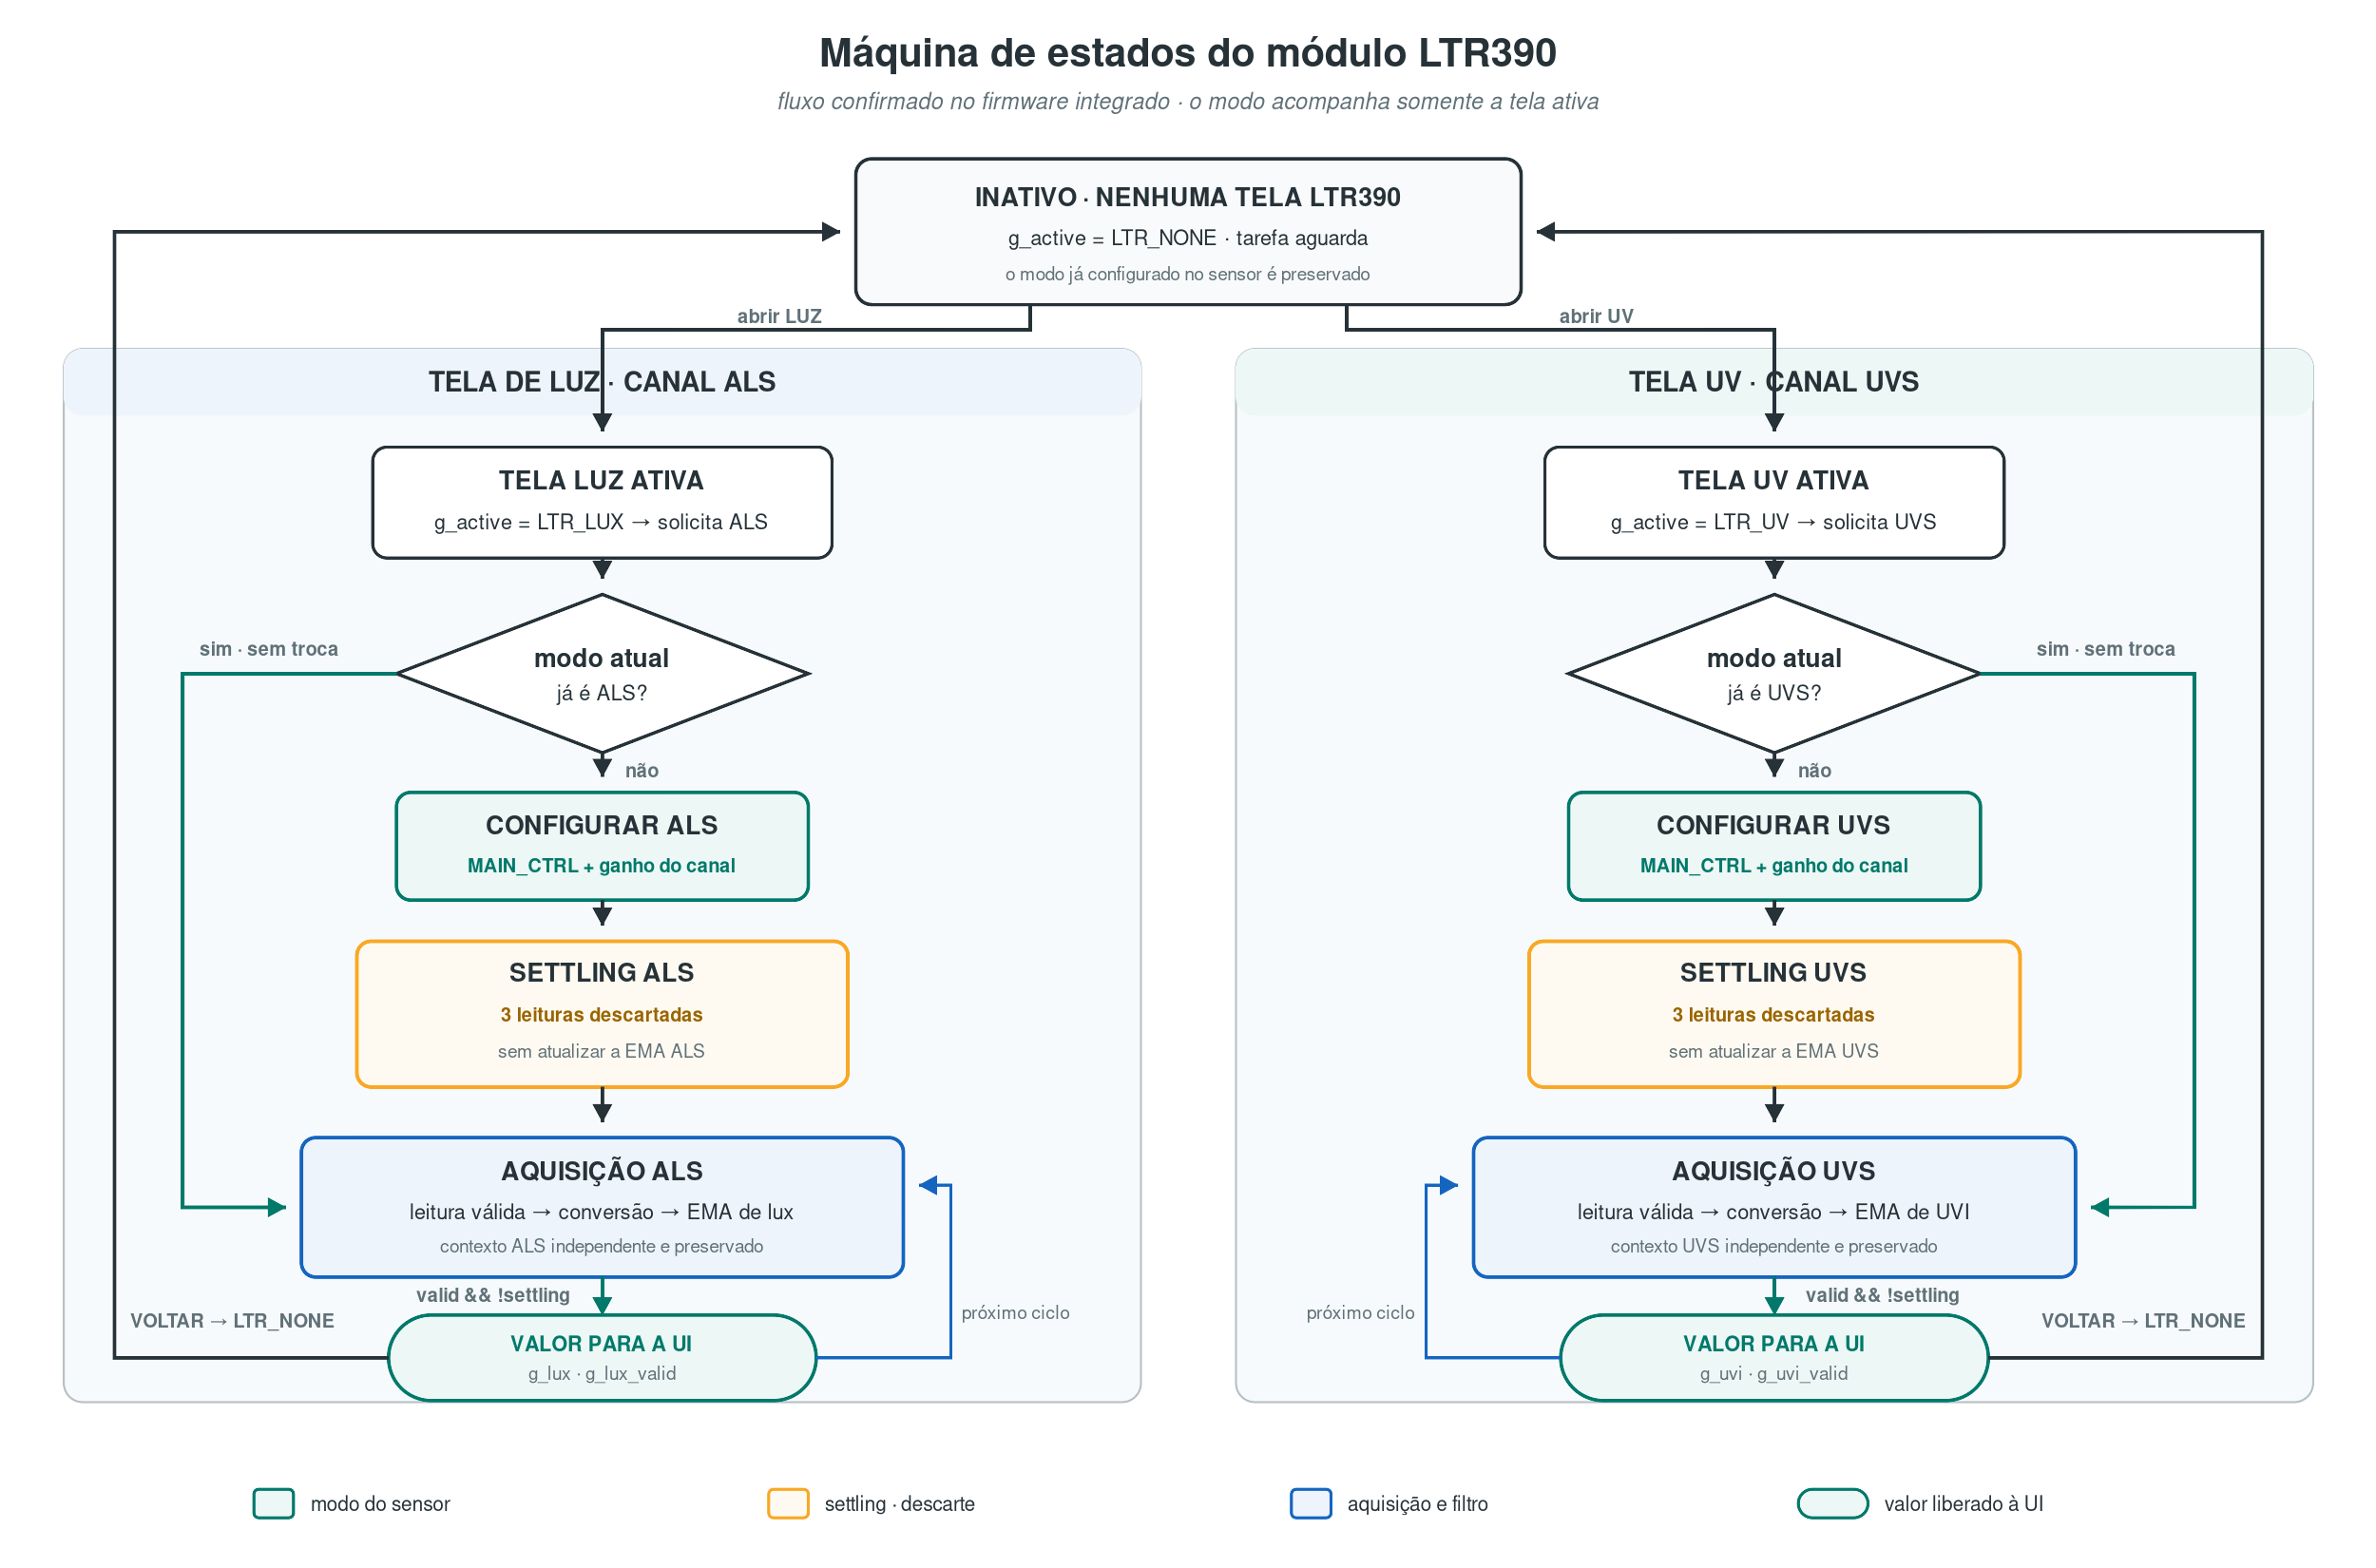
\includegraphics[width=0.98\textwidth]{Diagramas/teoricas/ltr390_maquina_estados.png}
\fonteelemento{Elaborado pelo autor a partir de \texttt{ltr390\_screen.c} e \texttt{ltr390\_process.c}}
\end{figure}


\subsubsection{Convers\~ao para lux e UVI}


Na configura\c{c}\~ao consolidada, a ilumin\^ancia \'e calculada por


\[
E_v=0{,}2\,N_{\mathrm{ALS}},
\]


em que $N_{\mathrm{ALS}}$ \'e a contagem bruta. A estimativa de UVI \'e calculada por


\[
\widehat{\mathrm{UVI}}=\frac{N_{\mathrm{UVS}}}{575}.
\]


Os fatores dependem de ganho e tempo de integra\c{c}\~ao. Por isso, as fun\c{c}\~oes de convers\~ao permanecem associadas \`a configura\c{c}\~ao usada pelo driver e dever\~ao ser atualizadas em conjunto caso esses par\^ametros mudem.


\subsubsection{Remo\c{c}\~ao do SW\_RESET}


A sequ\^encia inicial executava o comando de reinicializa\c{c}\~ao por software. O dispositivo deixava de responder antes de confirmar a escrita, produzindo NACK em uma opera\c{c}\~ao que, no teste isolado, podia parecer apenas uma particularidade local. No barramento compartilhado, esse erro afetava as transa\c{c}\~oes seguintes.


Como todos os registradores necess\'arios j\'a eram programados explicitamente, o comando foi removido da inicializa\c{c}\~ao. A recupera\c{c}\~ao do I$^2$C continua dispon\'ivel para falhas reais, mas n\~ao \'e usada para conservar uma opera\c{c}\~ao desnecess\'aria que produz erro previs\'ivel.


\subsubsection{Integra\c{c}\~ao com tarefa e tela}


A tarefa observa qual das telas do m\'odulo est\'a ativa, configura o modo correspondente, aguarda a estabiliza\c{c}\~ao e publica o valor convertido. Cada canal mant\'em seu estado de filtragem por m\'edia m\'ovel exponencial, com $\alpha=0{,}3$.


Erros de comunica\c{c}\~ao n\~ao s\~ao convertidos em zero. A tela distingue indisponibilidade de uma leitura v\'alida de baixa ilumin\^ancia ou baixa resposta ultravioleta.


\subsection{M\'odulo de b\'ussola}


\subsubsection{Bypass e inicializa\c{c}\~ao}


O driver inicializa o MPU-9250 em 0x68 e habilita o \emph{bypass} para expor o AK8963 em 0x0C ao controlador principal. Em seguida, verifica a identidade do magnet\^ometro e configura seu modo de aquisi\c{c}\~ao. Todo o fluxo utiliza o mesmo mutex e o mesmo servi\c{c}o de recupera\c{c}\~ao dos demais dispositivos.


Na leitura, os registradores de estado s\~ao consultados antes dos dados. O registrador ST2 \'e lido ao final para concluir a sequ\^encia e detectar transbordamento.


\subsubsection{ASA e convers\~ao}


Os coeficientes ASA armazenados de f\'abrica s\~ao lidos no modo apropriado do AK8963. Eles corrigem diferen\c{c}as de sensibilidade entre os eixos e s\~ao aplicados \`a convers\~ao das contagens para microteslas:


\[
m_i=\mathrm{raw}_i\frac{4912}{32760}ASA_i.
\]


O ajuste ASA n\~ao substitui a calibra\c{c}\~ao contra perturba\c{c}\~oes da montagem. Ap\'os essa convers\~ao, o m\'odulo aplica deslocamento e escala obtidos pelo procedimento executado no dispositivo.


\subsubsection{Calibra\c{c}\~ao}


A tela de calibra\c{c}\~ao divide o movimento necess\'ario em 12 setores. Durante a rota\c{c}\~ao do dispositivo, a tarefa acumula m\'inimos e m\'aximos de cada eixo e atualiza a indica\c{c}\~ao de cobertura. Ao concluir os setores, calcula para cada eixo o centro


\[
b_i=\frac{m_{i,\max}+m_{i,\min}}{2}.
\]


e uma escala relativa baseada nas meias-amplitudes observadas. Essa corre\c{c}\~ao representa deslocamento e escala por eixo; n\~ao implementa uma transforma\c{c}\~ao elipsoidal completa com termos cruzados.


O procedimento anterior baseado em exporta\c{c}\~ao CSV foi substitu\'ido pela calibra\c{c}\~ao executada na pr\'opria interface. A vers\~ao final n\~ao exige recompilar o firmware para aplicar novos par\^ametros.


A Figura~\ref{fig:calibracao-ondevice} separa o fluxo acionado pelo usu\'ario do c\'alculo posterior de \emph{heading} e mostra o caminho de cancelamento que preserva a calibra\c{c}\~ao v\'alida.


\begin{figure}[H]
\centering
\caption{Calibra\c{c}\~ao magn\'etica executada no prot\'otipo}
\label{fig:calibracao-ondevice}
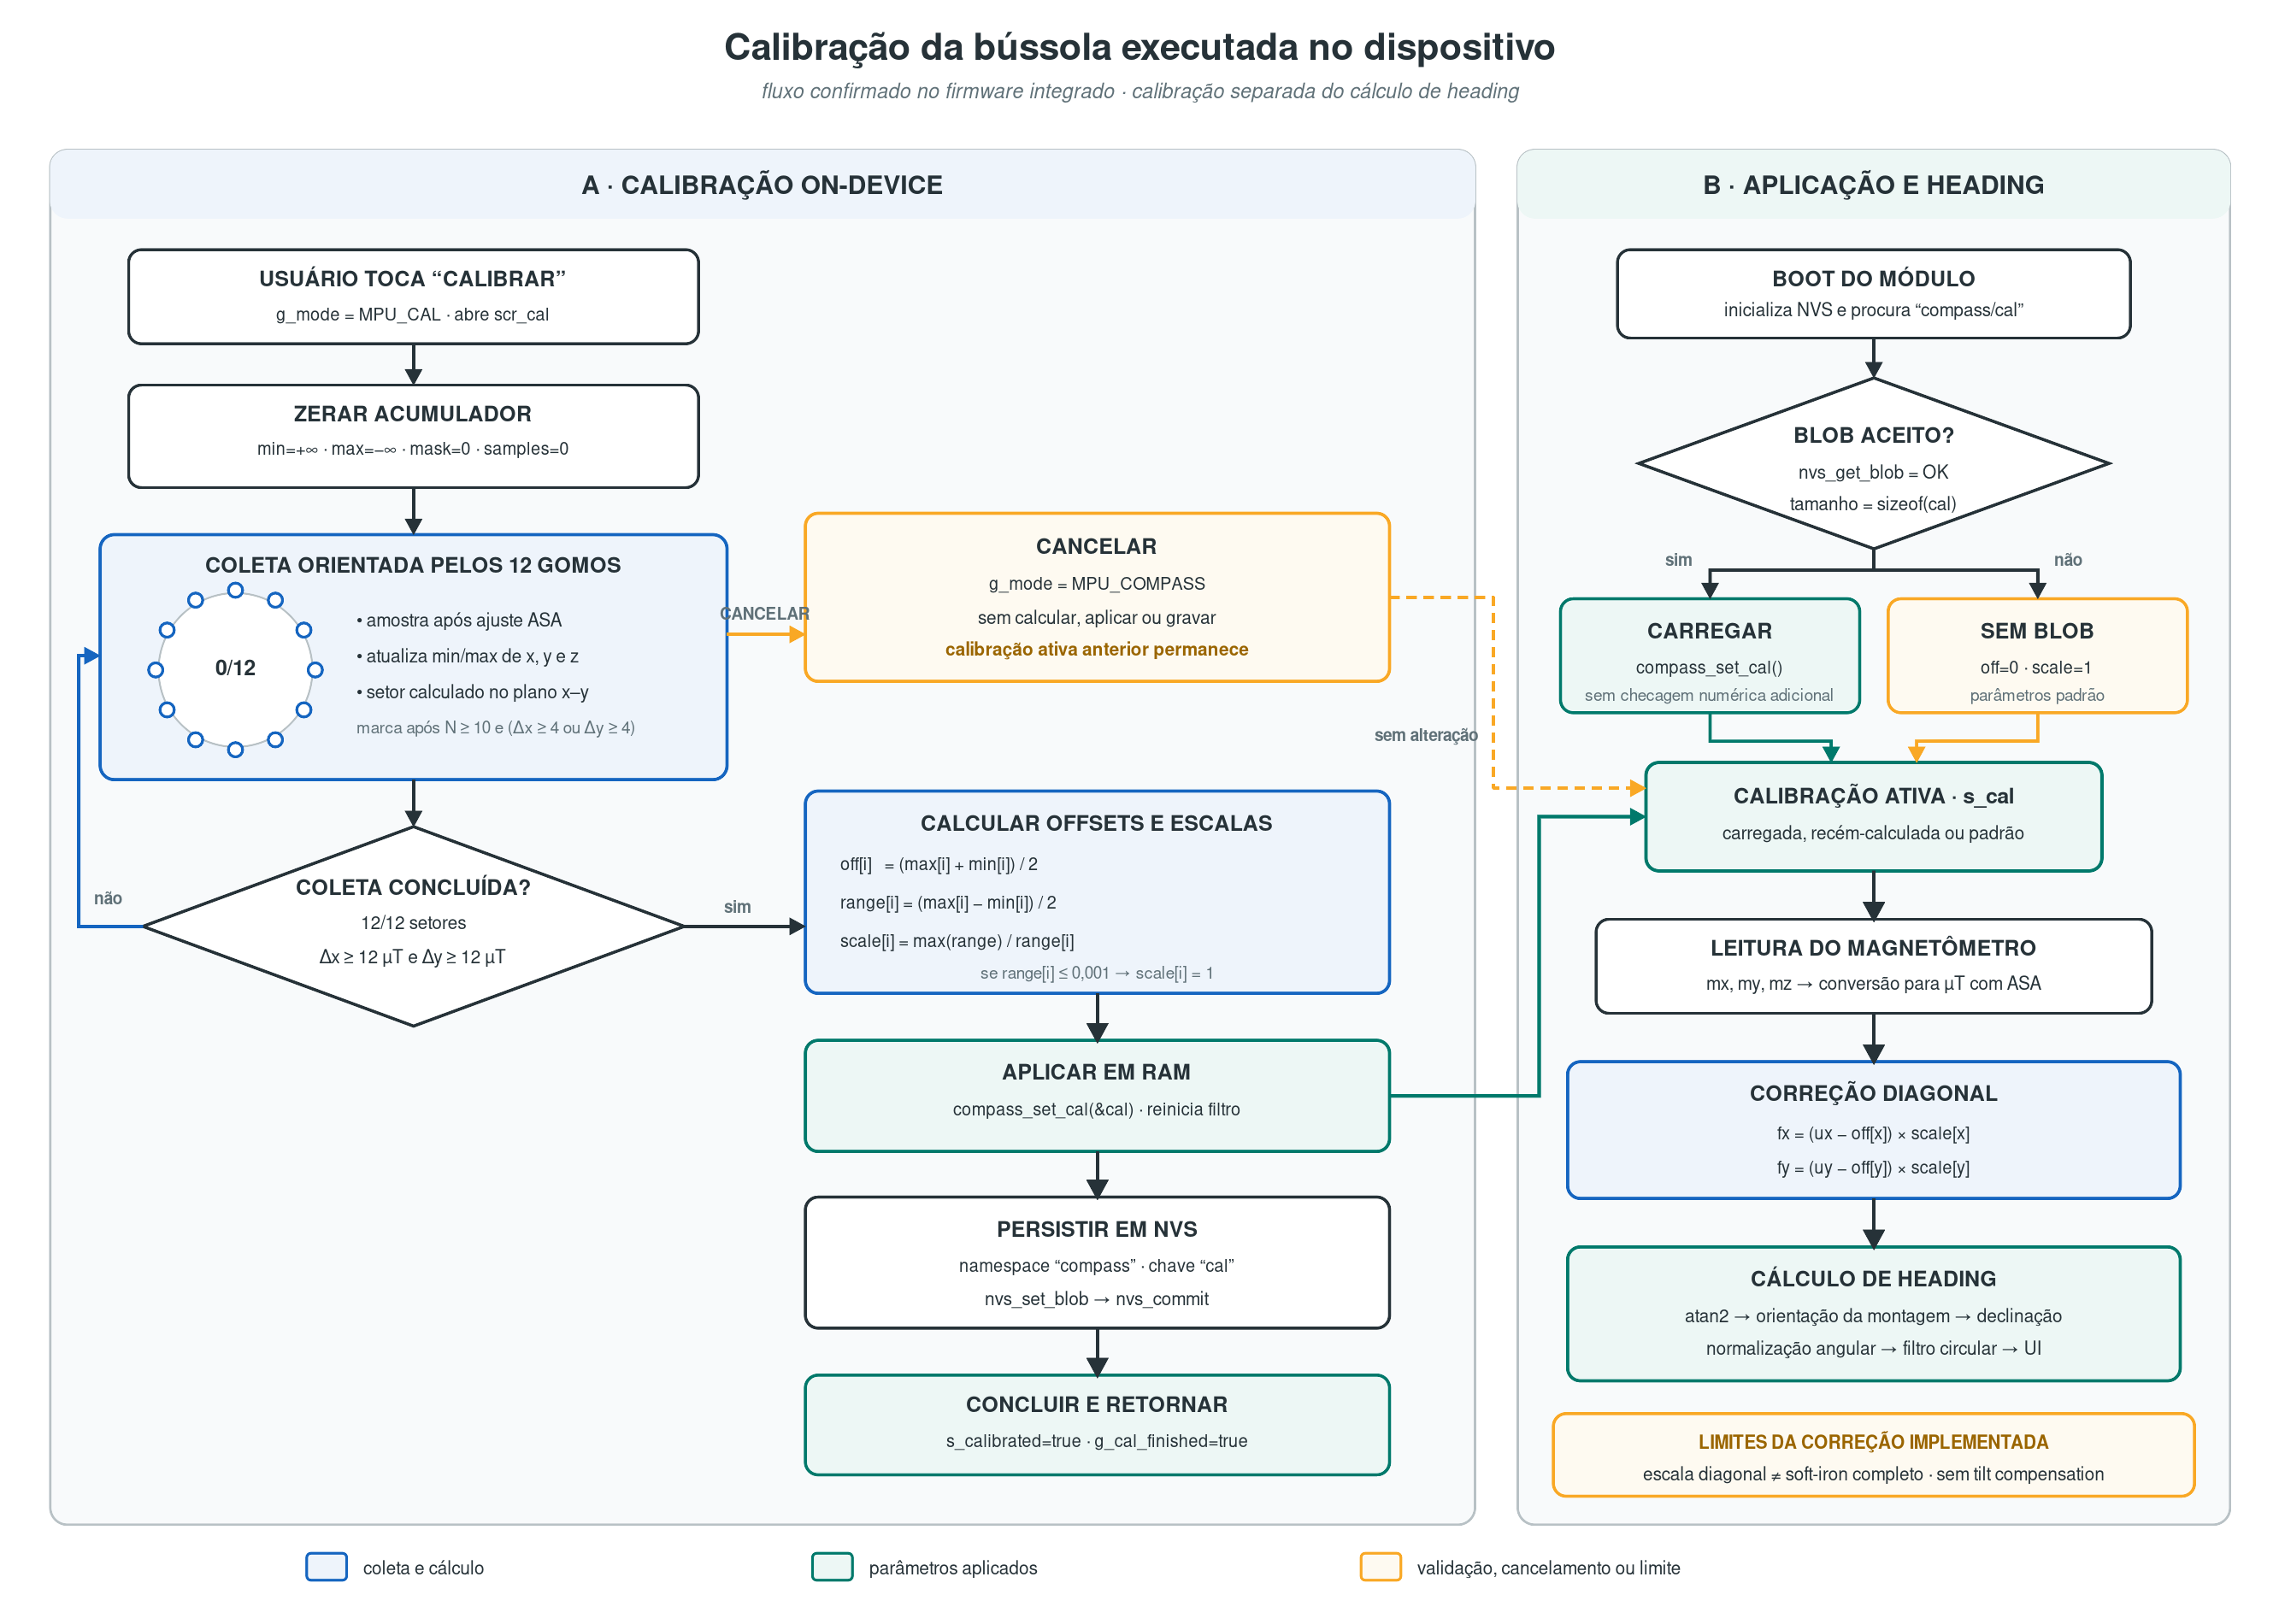
\includegraphics[width=0.98\textwidth]{Diagramas/teoricas/calibracao_bussola_ondevice.png}
\fonteelemento{Elaborado pelo autor a partir do processamento da b\'ussola, da tela de calibra\c{c}\~ao e da persist\^encia em NVS}
\end{figure}


\subsubsection{NVS}


Offsets, escalas e um indicador de validade s\~ao gravados na Non-Volatile Storage (NVS), mecanismo de armazenamento de pares chave-valor em flash fornecido pelo ESP-IDF (ESPRESSIF SYSTEMS, 2025h). Na inicializa\c{c}\~ao, o m\'odulo tenta carregar os valores e utiliza padr\~oes somente quando n\~ao h\'a conjunto v\'alido. Uma calibra\c{c}\~ao conclu\'ida substitui os dados anteriores de forma controlada.


A persist\^encia \'e restrita \`a b\'ussola. O contador do ped\^ometro n\~ao \'e restaurado ap\'os reinicializa\c{c}\~ao.


\subsubsection{Heading e filtro}


Ap\'os aplicar ASA e calibra\c{c}\~ao, o m\'odulo ajusta o mapeamento dos eixos \`a orienta\c{c}\~ao f\'isica da placa e calcula


\[
\psi=\operatorname{atan2}(m_y,-m_x).
\]


O resultado \'e normalizado para o intervalo de 0$^\circ$ a 360$^\circ$. Um filtro com $\alpha=0{,}15$ trata a diferen\c{c}a angular pelo caminho mais curto, evitando uma m\'edia incorreta entre valores pr\'oximos de 359$^\circ$ e 1$^\circ$.


A implementa\c{c}\~ao inverte o sentido de rota\c{c}\~ao devido \`a montagem, acrescenta 180$^\circ$ de orienta\c{c}\~ao f\'isica e aplica declina\c{c}\~ao fixa de $-21^\circ$, conforme os par\^ametros compilados. A tela converte o \^angulo nas oito dire\c{c}\~oes cardeais e intercardeais. N\~ao h\'a compensa\c{c}\~ao de inclina\c{c}\~ao, de modo que a indica\c{c}\~ao pressup\~oe o dispositivo aproximadamente nivelado; a declina\c{c}\~ao fixa tamb\'em deve ser atualizada para outro local ou \'epoca.


\subsubsection{Integra\c{c}\~ao com tarefa e tela}


A tarefa da b\'ussola e a tarefa do ped\^ometro s\~ao distintas, embora ambas acessem o mesmo MPU-9250 por meio do mutex compartilhado. Quando a b\'ussola est\'a ativa, sua tarefa l\^e o magnet\^ometro a cada 60 ms, atualiza o \emph{heading} e responde a comandos de calibra\c{c}\~ao. A tela apresenta \^angulo, dire\c{c}\~ao e estado dos par\^ametros persistidos.


\subsection{M\'odulo de ped\^ometro}


\subsubsection{Tentativa com DMP}


A primeira abordagem procurou utilizar o Digital Motion Processor (DMP) do MPU-9250. Ela exigia carregar firmware no dispositivo por registradores de mem\'oria. Na combina\c{c}\~ao de m\'odulo e implementa\c{c}\~ao testada, esses acessos produziram NACK e impediram concluir a inicializa\c{c}\~ao.


O ocorrido n\~ao demonstra incompatibilidade geral do DMP com o ESP32-C6. Diante do custo de investigar uma depend\^encia adicional e da necessidade de controlar o algoritmo, optou-se por um ped\^ometro implementado no firmware principal.


\subsubsection{Algoritmo pr\'oprio}


O algoritmo utiliza apenas o aceler\^ometro do MPU-9250. O girosc\'opio permanece desligado para essa fun\c{c}\~ao. As amostras dos tr\^es eixos s\~ao convertidas para unidades de $g$, combinadas pela magnitude e processadas por um detector de eventos.


O acesso ao aceler\^ometro fica na camada de hardware do m\'odulo, enquanto filtragem e contagem permanecem na camada de processamento. A tarefa coordena as duas sem transferir essas responsabilidades ao n\'ucleo.


\subsubsection{Configura\c{c}\~ao}


O aceler\^ometro opera na faixa de $\pm2g$, com fator de convers\~ao de 16.384 contagens por $g$, e \'e amostrado a 50 Hz. O per\'iodo de 20 ms \'e compat\'ivel com a resolu\c{c}\~ao de 10 ms do \emph{tick} configurado.


\subsubsection{Magnitude, EMA, limiar e intervalo m\'inimo}


A magnitude \'e calculada por


\[
a_m=\sqrt{a_x^2+a_y^2+a_z^2}.
\]


Uma m\'edia m\'ovel exponencial com $\alpha=0{,}2$ reduz componentes r\'apidas. Um passo \'e reconhecido quando o sinal cruza o limiar de 1,15 $g$, respeitando uma histerese de 0,05 $g$. Depois de uma detec\c{c}\~ao, novos eventos s\~ao ignorados por 300 ms, limitando contagens m\'ultiplas do mesmo movimento.


Os par\^ametros s\~ao fixos e foram escolhidos durante o desenvolvimento. Sua adequa\c{c}\~ao a ritmos e usu\'arios diferentes permanece dependente do ensaio controlado de pedometria.


A arquitetura compartilhada entre b\'ussola e ped\^ometro \'e mostrada na Figura~\ref{fig:mpu9250-modulo}. O detector implementado segue a rela\c{c}\~ao conceitual entre limiar, histerese e intervalo refrat\'ario apresentada na Figura~\ref{fig:pedometro-limiar}, na fundamenta\c{c}\~ao te\'orica.


\begin{figure}[H]
\centering
\caption{Arquitetura do m\'odulo MPU-9250}
\label{fig:mpu9250-modulo}
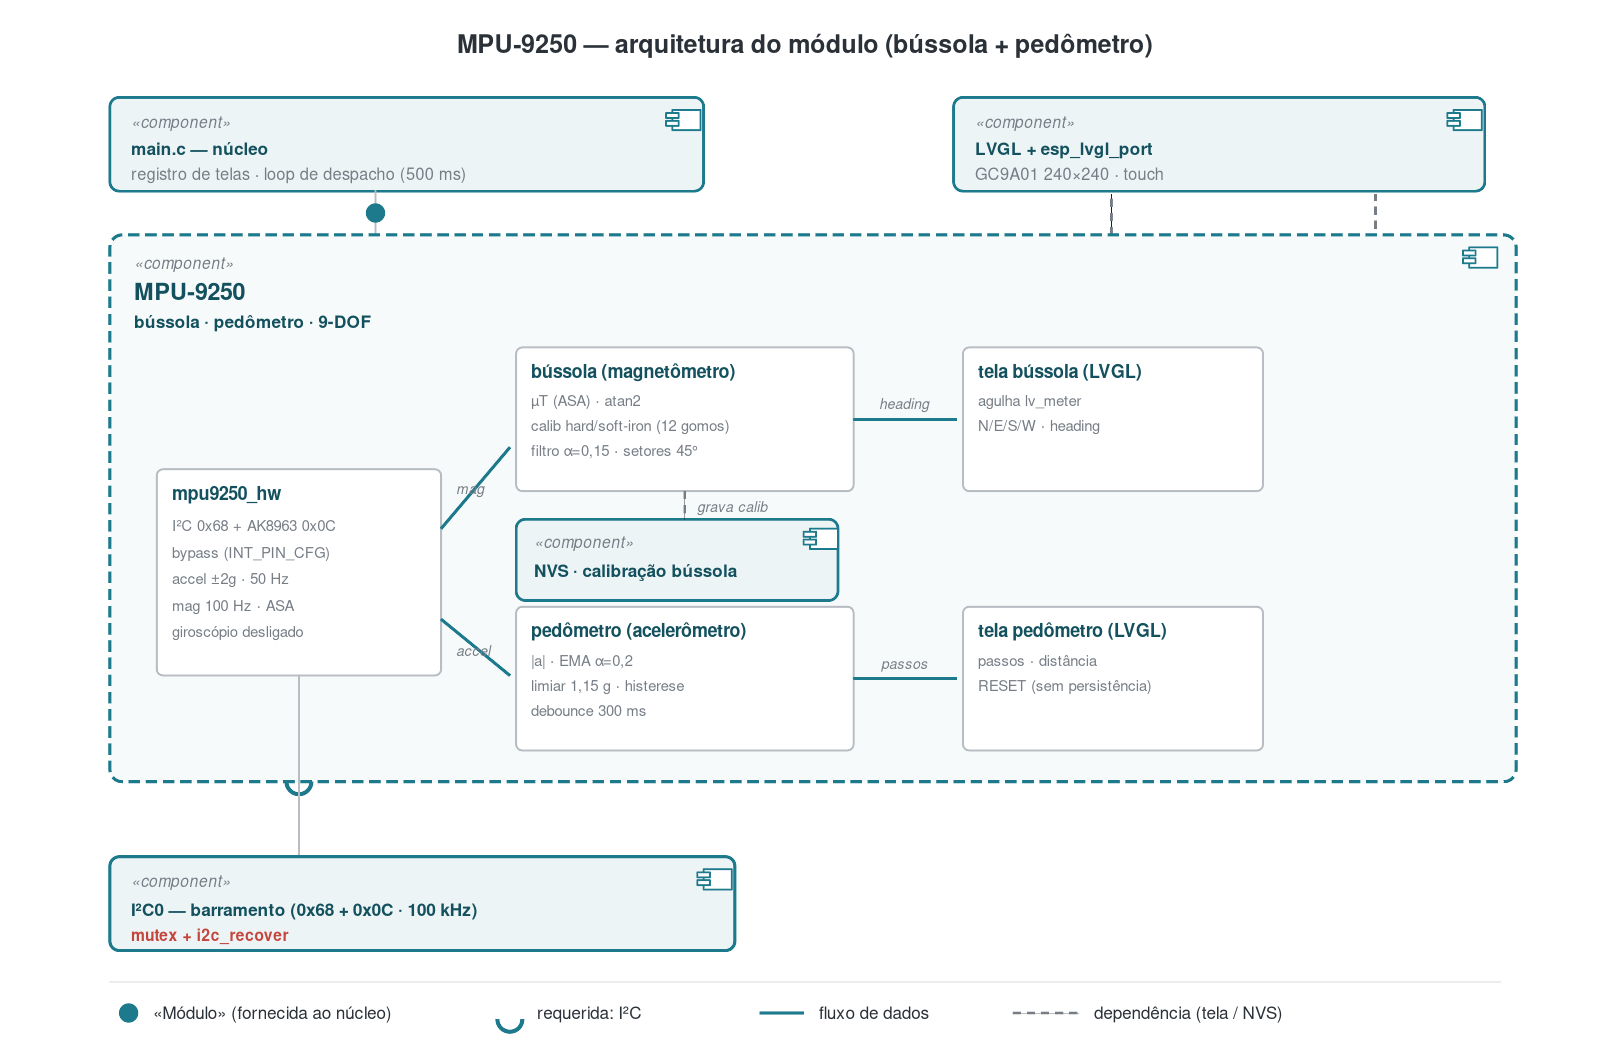
\includegraphics[width=0.96\textwidth]{Diagramas/mpu9250/mpu9250_modulo.png}
\fonteelemento{Elaborado pelo autor a partir de \texttt{pedometer\_process.c} e \texttt{pedometer\_screen.c}}
\end{figure}


\subsubsection{Dist\^ancia estimada}


A dist\^ancia apresentada \'e o produto do n\'umero de passos por um comprimento fixo de 0,70 m:


\[
\widehat d=0{,}70N_{\mathrm{passos}}.
\]


Esse valor n\~ao \'e individualizado por estatura ou padr\~ao de marcha. A interface o identifica como estimativa derivada do contador.


\subsubsection{Integra\c{c}\~ao com tarefa e tela}


A tarefa coleta acelera\c{c}\~ao quando a tela do ped\^ometro est\'a ativa, atualiza o detector e publica passos e dist\^ancia. A tela oferece comando para zerar a sess\~ao. O estado permanece em mem\'oria vol\'atil e retorna a zero ap\'os reinicializa\c{c}\~ao.


\subsection{Uso de mem\'oria e otimiza\c{c}\~oes}


A parti\c{c}\~ao de aplica\c{c}\~ao foi mantida em 1 MiB. A compila\c{c}\~ao limpa da vers\~ao final do bin\'ario produziu um arquivo de 784.240 bytes (765,86 KiB), equivalente a 74,79\% da parti\c{c}\~ao. A contribui\c{c}\~ao incremental de cada m\'odulo ainda n\~ao foi medida por compila\c{c}\~oes controladas.


O pool interno do LVGL foi configurado para 96 KiB. A configura\c{c}\~ao anterior de 32 KiB n\~ao comportava a cria\c{c}\~ao dos objetos da b\'ussola, especialmente o medidor gr\'afico. Esse ajuste aumenta a mem\'oria reservada \`a interface e precisa ser considerado junto ao heap dispon\'ivel.


Uma imagem RGB565 de 240 $\times$ 240 pixels requer ao menos 115.200 bytes sem transpar\^encia; recursos convertidos podem acrescentar cabe\c{c}alho, alinhamento ou outro formato. Para evitar repetir esse custo em cada tela, a interface utiliza widgets, formas e fontes com subconjuntos de glifos.


\subsection{Persist\^encia}


A NVS armazena os par\^ametros de calibra\c{c}\~ao da b\'ussola. O RTC mant\'em data e hora em seu pr\'oprio dom\'inio de alimenta\c{c}\~ao, com bateria de reserva. Esses dois mecanismos possuem ciclos de vida distintos: a NVS conserva par\^ametros do firmware, enquanto o PCF8563 mant\'em a base de calend\'ario.


O ped\^ometro n\~ao possui persist\^encia, e valores instant\^aneos dos sensores n\~ao s\~ao gravados. O projeto tamb\'em n\~ao implementa hist\'orico de medi\c{c}\~oes, armazenamento em cart\~ao microSD ou sincroniza\c{c}\~ao remota. Essas aus\^encias limitam o escopo do estado persistente e evitam atribuir ao prot\'otipo fun\c{c}\~oes de registro que n\~ao foram implementadas.

\clearpage
\section{Resultados e Discuss\~ao}


Este cap\'itulo re\'une os resultados atualmente documentados sobre a plataforma e discute seu alcance.


O firmware integrado, o caderno de ensaios, as fotografias dos instrumentos dispon\'iveis, os relat\'orios de compila\c{c}\~ao e as figuras dos resultados funcionais foram incorporados ao reposit\'orio. A montagem provis\'oria foi documentada por descri\c{c}\~ao e mapa de liga\c{c}\~oes, sem fotografia panor\^amica adicional.

Extensibilidade e acoplamento foram avaliados estruturalmente; a mem\'oria global foi medida; a inicializa\c{c}\~ao degradada foi verificada qualitativamente; e os testes funcionais dos sensores, RTC, consumo de corrente e condicionamento PPG foram incorporados. Permaneceram fora do escopo final a mem\'oria incremental por m\'odulo, CPU e heap por cen\'ario e a efic\'acia din\^amica da recupera\c{c}\~ao I$^2$C sob falha induzida, limita\c{c}\~oes explicitadas nas se\c{c}\~oes correspondentes.


\subsection{Estado das evid\^encias}


Para evitar atribuir a mesma for\c{c}a a registros distintos, as evid\^encias foram classificadas nos tr\^es n\'iveis apresentados no Quadro~\ref{qua:niveis-evidencia}.


\begin{quadro}[H]
\centering
\caption{Classifica\c{c}\~ao das evid\^encias empregadas}
\label{qua:niveis-evidencia}
\small
\begin{tabularx}{\textwidth}{|>{\raggedright\arraybackslash}p{0.20\textwidth}|>{\raggedright\arraybackslash}p{0.34\textwidth}|>{\raggedright\arraybackslash}X|}
\hline
\textbf{N\'ivel} & \textbf{Descri\c{c}\~ao} & \textbf{Uso neste cap\'itulo} \\
\hline
evid\^encia prim\'aria & firmware, log, tabela, s\'erie temporal, fotografia ou arquivo de ensaio dispon\'ivel & base para resultado reproduz\'ivel \\
\hline
registro consolidado & valor resumido nos documentos de controle ou nos compilados, sem dado prim\'ario dispon\'ivel & resultado provis\'orio a conferir \\
\hline
observa\c{c}\~ao funcional & relato de bancada sem procedimento completo, instrumento identificado ou repeti\c{c}\~oes & demonstra funcionamento, n\~ao desempenho quantitativo \\
\hline
\end{tabularx}
\fonteelemento{Elaborado pelo autor}
\end{quadro}


O caderno de ensaios e as figuras associadas fornecem evid\^encias prim\'arias para os testes funcionais dos sensores, do RTC e do consumo de corrente. Os resultados arquiteturais permanecem predominantemente apoiados na implementa\c{c}\~ao e em registros consolidados.


\subsection{Prot\'otipo integrado}


Os documentos de consolida\c{c}\~ao descrevem um prot\'otipo formado pelo XIAO ESP32-C6 encaixado no Round Display e por quatro unidades sensoriais externas: MAX30102, DS18B20, LTR390 e MPU-9250/AK8963. A interface inclui tela principal, navega\c{c}\~ao por toque e telas dedicadas \`as fun\c{c}\~oes. O RTC PCF8563 mant\'em data e hora.


A integra\c{c}\~ao combina SPI2 para o display, I$^2$C compartilhado para toque, RTC e sensores e 1-Wire por RMT para temperatura. Esse conjunto demonstra funcionalmente que a plataforma comporta dispositivos com transportes e ciclos de aquisi\c{c}\~ao diferentes.


A fotografia da placa em opera\c{c}\~ao, as renderiza\c{c}\~oes e o mapa de liga\c{c}\~oes foram apresentados em Materiais e M\'etodos. N\~ao se repete aqui a mesma evid\^encia visual, pois a configura\c{c}\~ao sensorial avaliada corresponde \`aquela montagem.


\subsection{Cumprimento dos requisitos}


A s\'intese do Quadro~\ref{qua:estado-requisitos} separa implementa\c{c}\~ao confirmada, teste funcional e limita\c{c}\~ao de avalia\c{c}\~ao.


\begin{quadro}[H]
\centering
\caption{Estado dos requisitos da plataforma}
\label{qua:estado-requisitos}
\small
\begin{tabularx}{\textwidth}{|>{\raggedright\arraybackslash}p{0.23\textwidth}|>{\raggedright\arraybackslash}p{0.25\textwidth}|>{\raggedright\arraybackslash}X|}
\hline
\textbf{Requisito} & \textbf{Estado documentado} & \textbf{Evid\^encia dispon\'ivel} \\
\hline
contrato de m\'odulos & implementado & descri\c{c}\~ao consolidada de inicializa\c{c}\~ao, cria\c{c}\~ao e exibi\c{c}\~ao de tela \\
\hline
integra\c{c}\~ao dos sensores & testada funcionalmente & caderno de ensaios, tabelas e figuras dos m\'odulos \\
\hline
navega\c{c}\~ao por toque & testada funcionalmente & compilado do Round Display e resumo consolidado \\
\hline
compartilhamento do I$^2$C & implementado & mapa consolidado, mutex e servi\c{c}o de recupera\c{c}\~ao descritos \\
\hline
inicializa\c{c}\~ao n\~ao fatal & implementada & descri\c{c}\~ao arquitetural \\
\hline
extensibilidade & prevista e implementada arquiteturalmente & contrato e pontos de registro descritos \\
\hline
toler\^ancia a falhas & mecanismos implementados & inicializa\c{c}\~ao n\~ao fatal e recupera\c{c}\~ao p\'os-NACK descritas \\
\hline
uso de recursos & parcialmente registrado & tamanho integrado e pool do LVGL nos documentos \\
\hline
fun\c{c}\~oes sensoriais & testadas funcionalmente & compara\c{c}\~oes funcionais e ensaios controlados registrados \\
\hline
\end{tabularx}
\fonteelemento{Elaborado pelo autor a partir do firmware e do caderno de ensaios}
\end{quadro}


O quadro permite afirmar que a arquitetura e os m\'odulos foram implementados, mas n\~ao que todos os objetivos de avalia\c{c}\~ao tenham sido cumpridos. Extensibilidade e acoplamento receberam uma avalia\c{c}\~ao estrutural retrospectiva; recursos computacionais e robustez din\^amica permanecem abertos.


\subsection{Arquitetura modular}


\subsubsection{Contrato dos m\'odulos}


Os registros indicam que MAX30102, DS18B20, LTR390 e as fun\c{c}\~oes baseadas no MPU-9250 foram integrados pelo mesmo ciclo de vida: inicializa\c{c}\~ao, cria\c{c}\~ao da tela e exibi\c{c}\~ao. O n\'ucleo registra telas e atualiza\c{c}\~oes, enquanto os algoritmos permanecem nos m\'odulos. O DS18B20 utiliza 1-Wire sem obrigar os demais componentes a conhecer esse transporte.


Essa evid\^encia \'e estrutural e mostra a presen\c{c}a de um ponto comum de integra\c{c}\~ao.

A confer\^encia do firmware mostrou que cada tela sensorial inclui \texttt{app.h} para registrar sua fun\c{c}\~ao de atualiza\c{c}\~ao. Os m\'odulos mant\^em estado em vari\'aveis est\'aticas locais ao arquivo e n\~ao acessam diretamente o estado de outros sensores. O n\'ucleo, entretanto, conhece explicitamente os cabe\c{c}alhos e os pontos de entrada de cada m\'odulo; a composi\c{c}\~ao n\~ao \'e din\^amica.


\subsubsection{Esfor\c{c}o de adi\c{c}\~ao de m\'odulo}

Como n\~ao foi integrado um componente novo durante a fase de avalia\c{c}\~ao, foi realizado um estudo retrospectivo do MAX30102. O projeto standalone possui 1307 linhas distribu\'idas em nove arquivos C e H; o m\'odulo integrado possui 1315 linhas em dez arquivos. Os seis arquivos de processamento \texttt{heart\_rate.c/.h}, \texttt{ppg\_filter.c/.h} e \texttt{spo2.c/.h}, totalizando 678 linhas, s\~ao id\^enticos nas duas vers\~oes.

O driver de hardware foi modificado para receber o barramento e o mutex compartilhados, recuperar o I$^2$C ap\'os erro e permitir ativa\c{c}\~ao e desligamento da aquisi\c{c}\~ao. As 294 linhas do \texttt{main.c} standalone foram substitu\'idas por 331 linhas em \texttt{max30102\_screen.c/.h}, que concentram tarefa, estado, callbacks, tela e interface p\'ublica. N\~ao foram encontradas altera\c{c}\~oes em outros m\'odulos sensoriais.

A integra\c{c}\~ao deixou seis pontos expl\'icitos fora da pasta do MAX30102: inclus\~ao do cabe\c{c}alho, callback de exibi\c{c}\~ao, item de menu, inicializa\c{c}\~ao, cria\c{c}\~ao da tela e diret\'orio de inclus\~ao no CMake. Assim, a estrutura concentra as mudan\c{c}as e preserva o processamento, mas n\~ao elimina edi\c{c}\~oes no n\'ucleo. Como o levantamento foi posterior \`a implementa\c{c}\~ao e n\~ao preservou o tempo de trabalho, ele caracteriza a estrutura da mudan\c{c}a, n\~ao o esfor\c{c}o temporal.


\subsubsection{Acoplamento e altera\c{c}\~oes no n\'ucleo}

A an\'alise dos cabe\c{c}alhos n\~ao encontrou depend\^encias diretas entre MAX30102, DS18B20 e LTR390. O ped\^ometro depende intencionalmente de \texttt{mpu9250\_hw}, pois reutiliza o aceler\^ometro da mesma unidade inercial. MAX30102, LTR390, MPU-9250 e RTC dependem do servi\c{c}o de recupera\c{c}\~ao do I$^2$C; o DS18B20 permanece fora desse barramento.

N\~ao foi identificado ciclo direto no grafo de inclus\~ao de cabe\c{c}alhos. No n\'ivel de pacotes existe uma depend\^encia bidirecional controlada: o n\'ucleo inclui as interfaces dos m\'odulos para comp\^o-los, enquanto as telas usam o contrato de \texttt{app.h} para registrar callbacks e obter servi\c{c}os comuns. Esse resultado \'e mais preciso do que classificar a arquitetura inteira como estritamente ac\'iclica. A Figura~\ref{fig:dependencias-firmware} apresenta o grafo obtido.

\begin{figure}[H]
\centering
\caption{Depend\^encias identificadas por an\'alise est\'atica do firmware integrado}
\label{fig:dependencias-firmware}
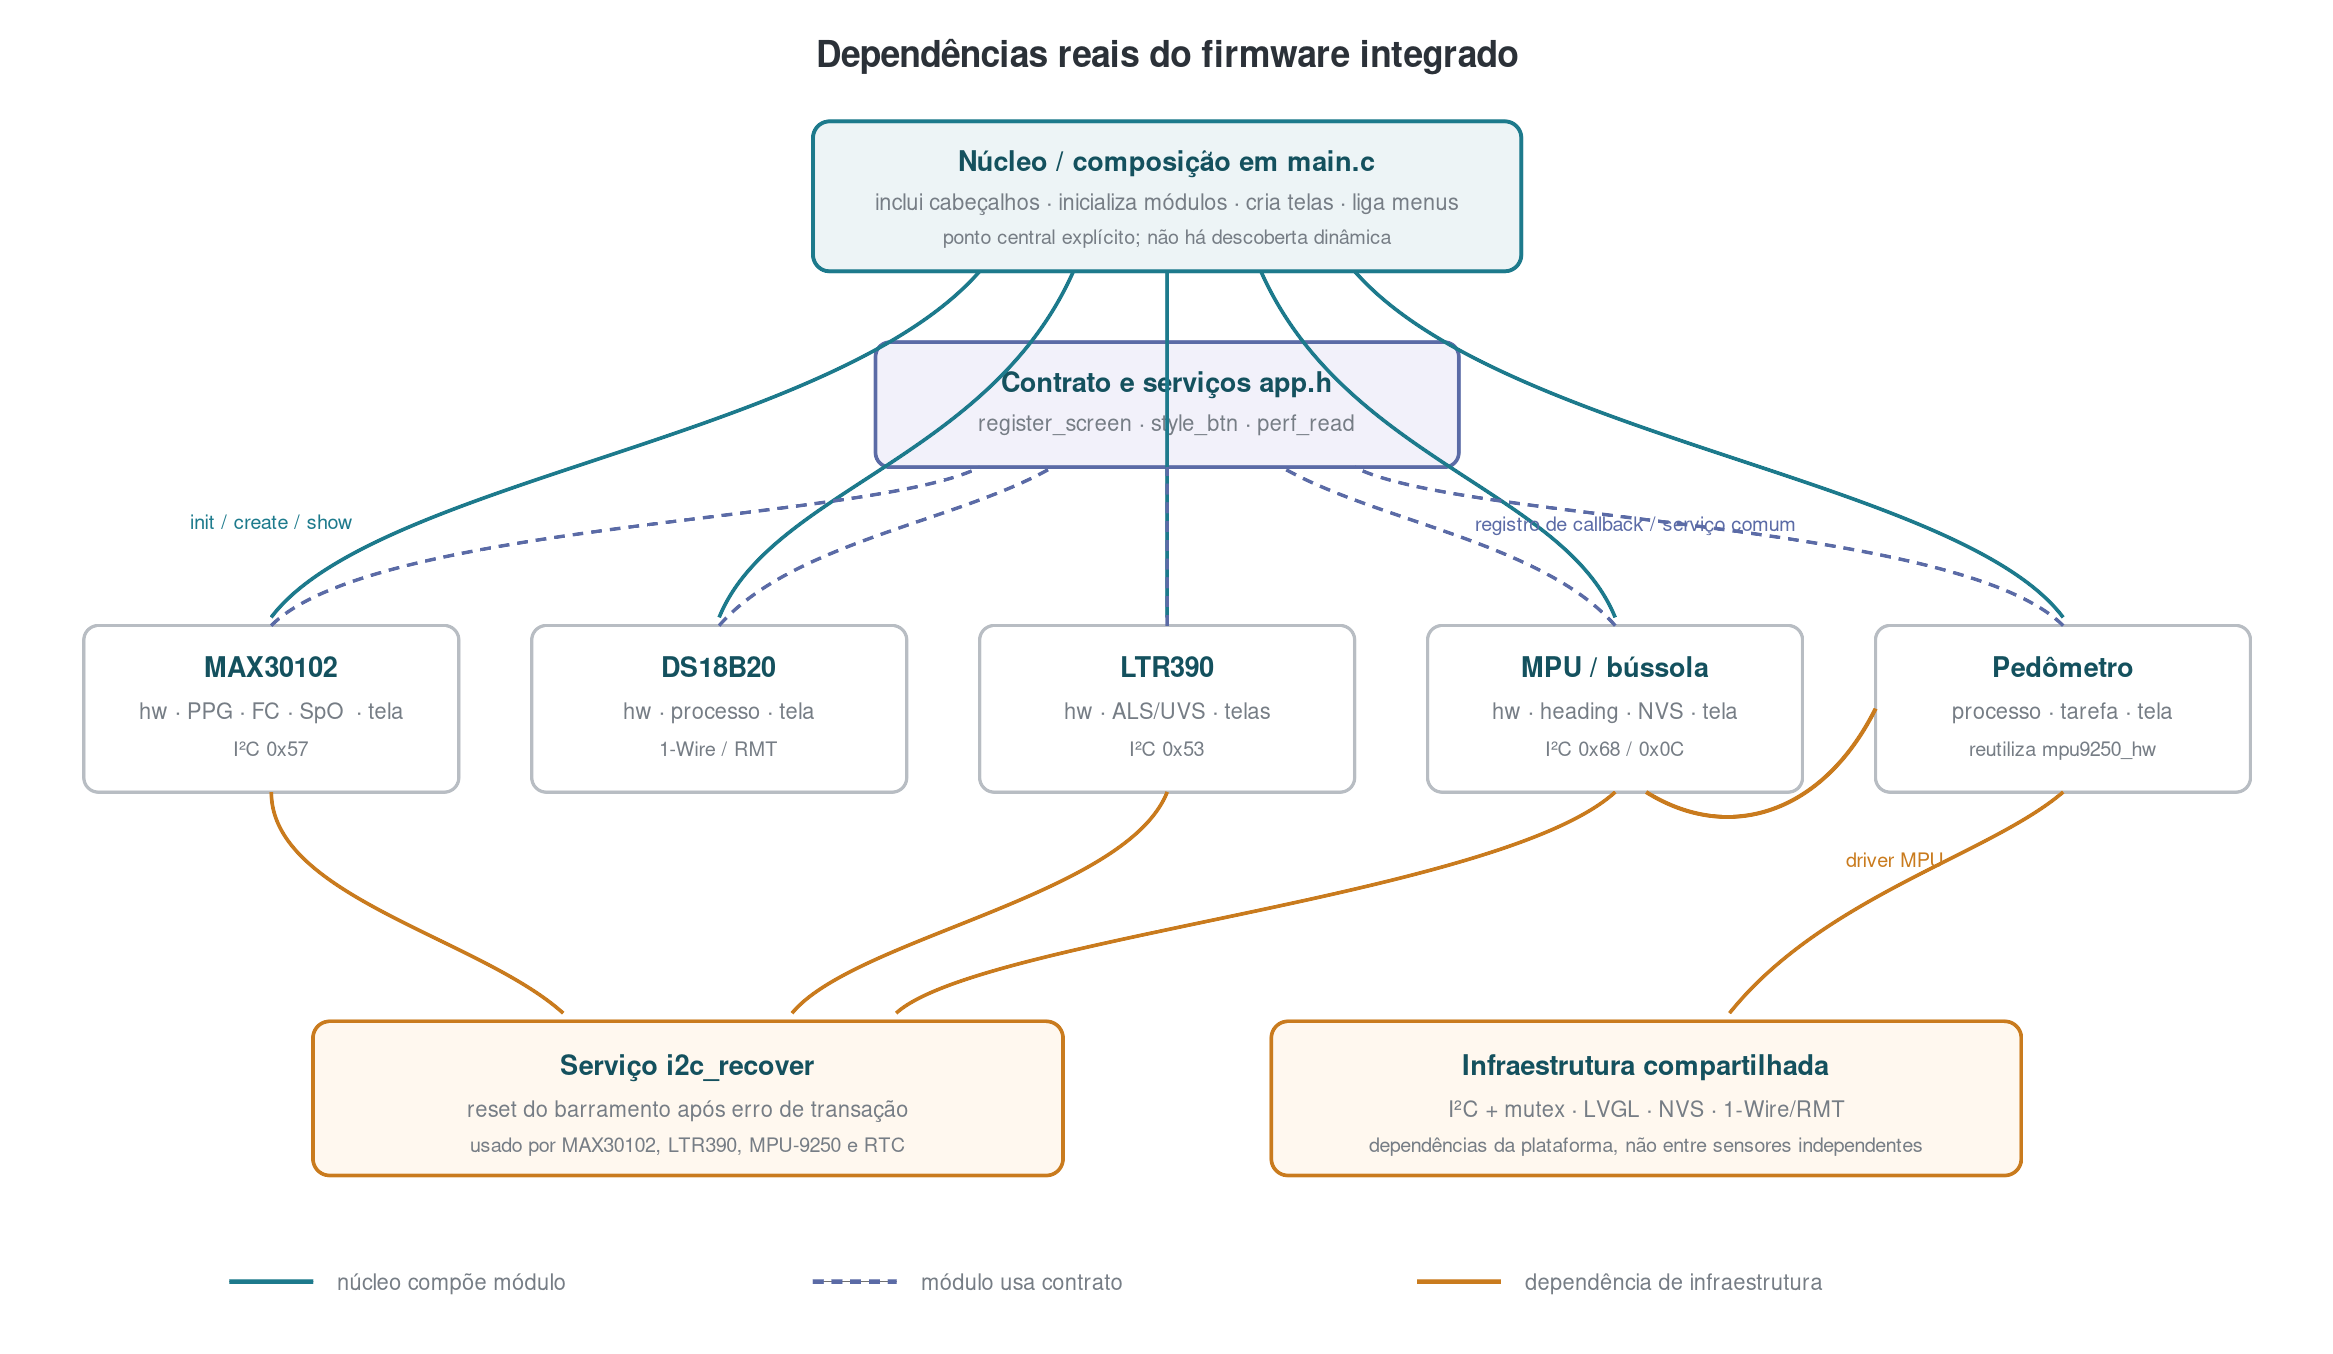
\includegraphics[width=0.98\textwidth]{Diagramas/sistema/dependencias_firmware.png}
\fonteelemento{Elaborado pelo autor a partir das inclus\~oes e chamadas do firmware}
\end{figure}


\subsection{Recursos computacionais}


\subsubsection{Tamanho do bin\'ario}


A vers\~ao final do bin\'ario avaliado foi obtida por uma compila\c{c}\~ao limpa e analisada com as ferramentas \texttt{size} e \texttt{size-components} do ESP-IDF v5.5.1.


O arquivo grav\'avel apresentou 784.240 bytes (765,86 KiB) em uma parti\c{c}\~ao de 1.048.576 bytes (1.024 KiB). Isso corresponde a 74,79\% de ocupa\c{c}\~ao e 264.336 bytes (258,14 KiB, ou 25,21\%) de folga; a sa\'ida resumida do ESP-IDF apresenta 25\%. A ferramenta \texttt{size} reportou imagem de 784.124 bytes, 116 bytes menor que o arquivo devido ao preenchimento do bin\'ario. O resultado confirma a ordem de grandeza anteriormente descrita como aproximadamente 760 KiB. A compara\c{c}\~ao com o registro anterior de 643 KB, contudo, n\~ao permite atribuir a diferen\c{c}a aos sensores, pois as vers\~oes podem diferir em fontes, componentes, otimiza\c{c}\~ao e recursos gr\'aficos.

Os relat\'orios completos de \texttt{size} e \texttt{size-components} foram preservados com os demais registros de an\'alise do trabalho.


\subsubsection{Mem\'oria por m\'odulo e heap}


O pool interno do LVGL foi configurado para 96 KiB depois que 32 KiB se mostraram insuficientes para criar os objetos da b\'ussola. Essa altera\c{c}\~ao documenta uma restri\c{c}\~ao de integra\c{c}\~ao.

O relat\'orio est\'atico registrou 179.360 bytes de DIRAM utilizados em 452.112 bytes considerados pela ferramenta, ou 39,67\%, com 272.752 bytes remanescentes. O total utilizado reuniu 105.632 bytes de BSS, 65.512 bytes de c\'odigo em DIRAM e 8.216 bytes de dados inicializados. Para flash, foram registrados 710.364 bytes de c\'odigo e constantes. No relat\'orio por bibliotecas, o LVGL respondeu por 361.202 bytes de contribui\c{c}\~ao ao ELF, incluindo 99.460 bytes de BSS, enquanto \texttt{libmain.a} reuniu 207.325 bytes. Esses valores de biblioteca n\~ao representam incrementos isolados dos sensores, e a DIRAM remanescente no mapa n\~ao equivale ao heap livre durante a execu\c{c}\~ao.


N\~ao foram executadas compila\c{c}\~oes incrementais nem coletas de heap por cen\'ario. Por isso, n\~ao se apresenta uma decomposi\c{c}\~ao gr\'afica por m\'odulo: produzi-la a partir do relat\'orio integrado atribuiria custos que os dados n\~ao permitem isolar.


\subsubsection{CPU e tempo de boot}

A ocupa\c{c}\~ao de CPU e o heap din\^amico n\~ao foram medidos de forma compar\'avel entre cen\'arios. A inspe\c{c}\~ao mostrou que \texttt{app\_perf\_read()} era chamada somente pela tela principal e comparava deltas do contador ocioso sem normalizar intervalos transcorridos quando outras telas permaneciam ativas. Os relat\'orios de compila\c{c}\~ao quantificam flash e mem\'oria est\'atica, mas n\~ao substituem medi\c{c}\~oes de CPU ou heap em execu\c{c}\~ao. Por isso, n\~ao se apresenta percentual de CPU nem se mant\'em a afirma\c{c}\~ao hist\'orica de carga inferior a 1\%.

Os tempos de boot dispon\'iveis pertencem ao piloto de inicializa\c{c}\~ao degradada descrito adiante. Como houve uma execu\c{c}\~ao registrada por condi\c{c}\~ao, os valores caracterizam os casos observados e n\~ao uma distribui\c{c}\~ao estat\'istica do tempo de inicializa\c{c}\~ao.


\subsection{Robustez e estabilidade}


\subsubsection{NACK e recupera\c{c}\~ao}


Os registros de desenvolvimento descrevem a implementa\c{c}\~ao de \texttt{i2c\_master\_bus\_\allowbreak reset()} ap\'os falhas e a remo\c{c}\~ao de uma opera\c{c}\~ao de \texttt{SW\_RESET} do LTR390 que produzia NACK previs\'ivel. Um erro de um m\'odulo foi, portanto, tratado como problema sist\^emico do recurso compartilhado.

A an\'alise est\'atica confirmou que os caminhos de erro dos drivers I$^2$C chamam o servi\c{c}o de recupera\c{c}\~ao antes de devolver o resultado da transa\c{c}\~ao. Essa evid\^encia demonstra a presen\c{c}a e a integra\c{c}\~ao do mecanismo no c\'odigo, mas n\~ao mede sua taxa de sucesso, sua lat\^encia nem a continuidade dos demais endere\c{c}os durante uma falha induzida. Como n\~ao foi realizado ensaio controlado de falha em opera\c{c}\~ao, a efic\'acia din\^amica da recupera\c{c}\~ao permanece uma limita\c{c}\~ao do trabalho.


\subsubsection{Sensor ausente}


A inicializa\c{c}\~ao n\~ao fatal foi avaliada com a remo\c{c}\~ao individual de cada sensor externo e, adicionalmente, com sensores ausentes em diversos arranjos. Em todas as condi\c{c}\~oes verificadas, o firmware concluiu a inicializa\c{c}\~ao e manteve operantes a tela principal, o toque, o RTC, os menus e a navega\c{c}\~ao.

As telas dependentes dos componentes removidos indicaram a indisponibilidade, enquanto os demais m\'odulos conectados permaneceram acess\'iveis e funcionais. Nenhuma remo\c{c}\~ao individual nem combina\c{c}\~ao ensaiada provocou \emph{panic}, disparo de watchdog, reinicializa\c{c}\~ao espont\^anea ou impedimento de uso do sistema principal. O resultado comprova funcionalmente a conten\c{c}\~ao da aus\^encia de sensores nas condi\c{c}\~oes testadas; como n\~ao houve protocolo estat\'istico de repeti\c{c}\~oes, n\~ao se atribui uma taxa num\'erica de disponibilidade.


\subsubsection{Transa\c{c}\~oes do toque}


O hist\'orico do Round Display atribui \`a leitura condicionada pelo pino de interrup\c{c}\~ao uma redu\c{c}\~ao substancial do tr\'afego I$^2$C e a interrup\c{c}\~ao do fluxo de NACK quando n\~ao havia toque. O firmware corrente confirma que o GPIO17 \'e consultado antes de iniciar a transa\c{c}\~ao.


A interpreta\c{c}\~ao segura \'e que o \emph{polling} incondicional produzia tr\'afego e erros excessivos, e que a consulta condicionada \`a interrup\c{c}\~ao reduziu ambos. Como o log bruto e a janela de contagem n\~ao foram localizados, os n\'umeros hist\'oricos de transa\c{c}\~oes por segundo foram exclu\'idos.


\subsubsection{Watchdog e ensaio prolongado}

O prot\'otipo permaneceu em opera\c{c}\~ao prolongada na tela principal sem travamento ou reinicializa\c{c}\~ao espont\^anea observada. A dura\c{c}\~ao exata e uma s\'erie temporal de heap n\~ao foram preservadas, e as telas sensoriais n\~ao permaneceram continuamente ativas durante essa observa\c{c}\~ao. O registro sustenta a estabilidade funcional observada da tela principal, mas n\~ao caracteriza um ensaio de estresse de todos os m\'odulos.


\subsubsection{Logs e RMT}


Os registros de desenvolvimento associam a emiss\~ao excessiva de mensagens I$^2$C a problemas temporais percebidos no DS18B20. A redu\c{c}\~ao dos n\'iveis de log foi mantida como corre\c{c}\~ao de depura\c{c}\~ao. Como n\~ao houve compara\c{c}\~ao controlada entre n\'iveis de log, n\~ao se atribui causalmente o comportamento do RMT \`a carga serial.


\subsection{MAX30102}


\subsubsection{Sinal bruto e filtrado}

Os canais infravermelho e vermelho foram registrados no teste standalone a 100 Hz, com sa\'ida CSV temporalmente alinhada e decimada para 50 Hz. O firmware registrou a detec\c{c}\~ao do dedo aos 12,122 s; o transiente de contato e converg\^encia do estimador de DC foi descartado. A an\'alise quantitativa empregou o intervalo de 20 a 73 s, totalizando 2.651 amostras. Nesse trecho, os n\'iveis brutos m\'edios foram 83.181 contagens no IR e 72.152 no vermelho, sem aproxima\c{c}\~ao da satura\c{c}\~ao do conversor de 18 bits.

O sinal AC filtrado apresentou amplitude pico a pico de 2.182 contagens no IR e 1.063 no vermelho, com valores RMS de 403 e 187 contagens, respectivamente. A correla\c{c}\~ao de Pearson entre os dois canais filtrados foi 0,955, indicando eventos puls\'ateis temporalmente coerentes nos dois comprimentos de onda. A maior componente espectral do IR na faixa de 0,5 a 3,3 Hz ocorreu em aproximadamente 1,40 Hz, equivalente a cerca de 84 BPM. A componente pr\'oxima de 2,9 Hz foi interpretada como segundo harm\^onico da forma de onda.

Ap\'os compensar duas amostras da sa\'ida a 50 Hz, a correla\c{c}\~ao entre o IR ap\'os remo\c{c}\~ao de DC e o IR filtrado foi 0,992, correspondendo a atraso observado de aproximadamente 40 ms. O RMS filtrado correspondeu a 98,1\% do RMS antes do passa-baixa no IR e a 98,0\% no vermelho. Na sa\'ida decimada, o desvio padr\~ao das diferen\c{c}\~oes entre amostras consecutivas diminuiu 23,9\% no IR e 24,9\% no vermelho. Entretanto, antes do passa-baixa, somente 2,2\% da energia espectral do IR e 2,7\% da energia do vermelho estavam acima de 5 Hz no trecho analisado. A pot\^encia entre 5 e 10 Hz foi reduzida em aproximadamente 5,7 dB nos dois canais. Portanto, o filtro limitou varia\c{c}\~oes mais r\'apidas, mas produziu altera\c{c}\~ao global discreta porque a maior parte do conte\'udo j\'a se encontrava abaixo de sua frequ\^encia de corte. A Figura~\ref{fig:ppg-condicionamento} re\'une a linha de base observada no intervalo longo e a compara\c{c}\~ao espectral do recorte de 30 a 40 s.

\begin{figure}[H]
\centering
\caption{Linha de base do canal infravermelho entre 15 e 73 s e compara\c{c}\~ao espectral antes e depois do passa-baixa no recorte de 30 a 40 s}
\label{fig:ppg-condicionamento}
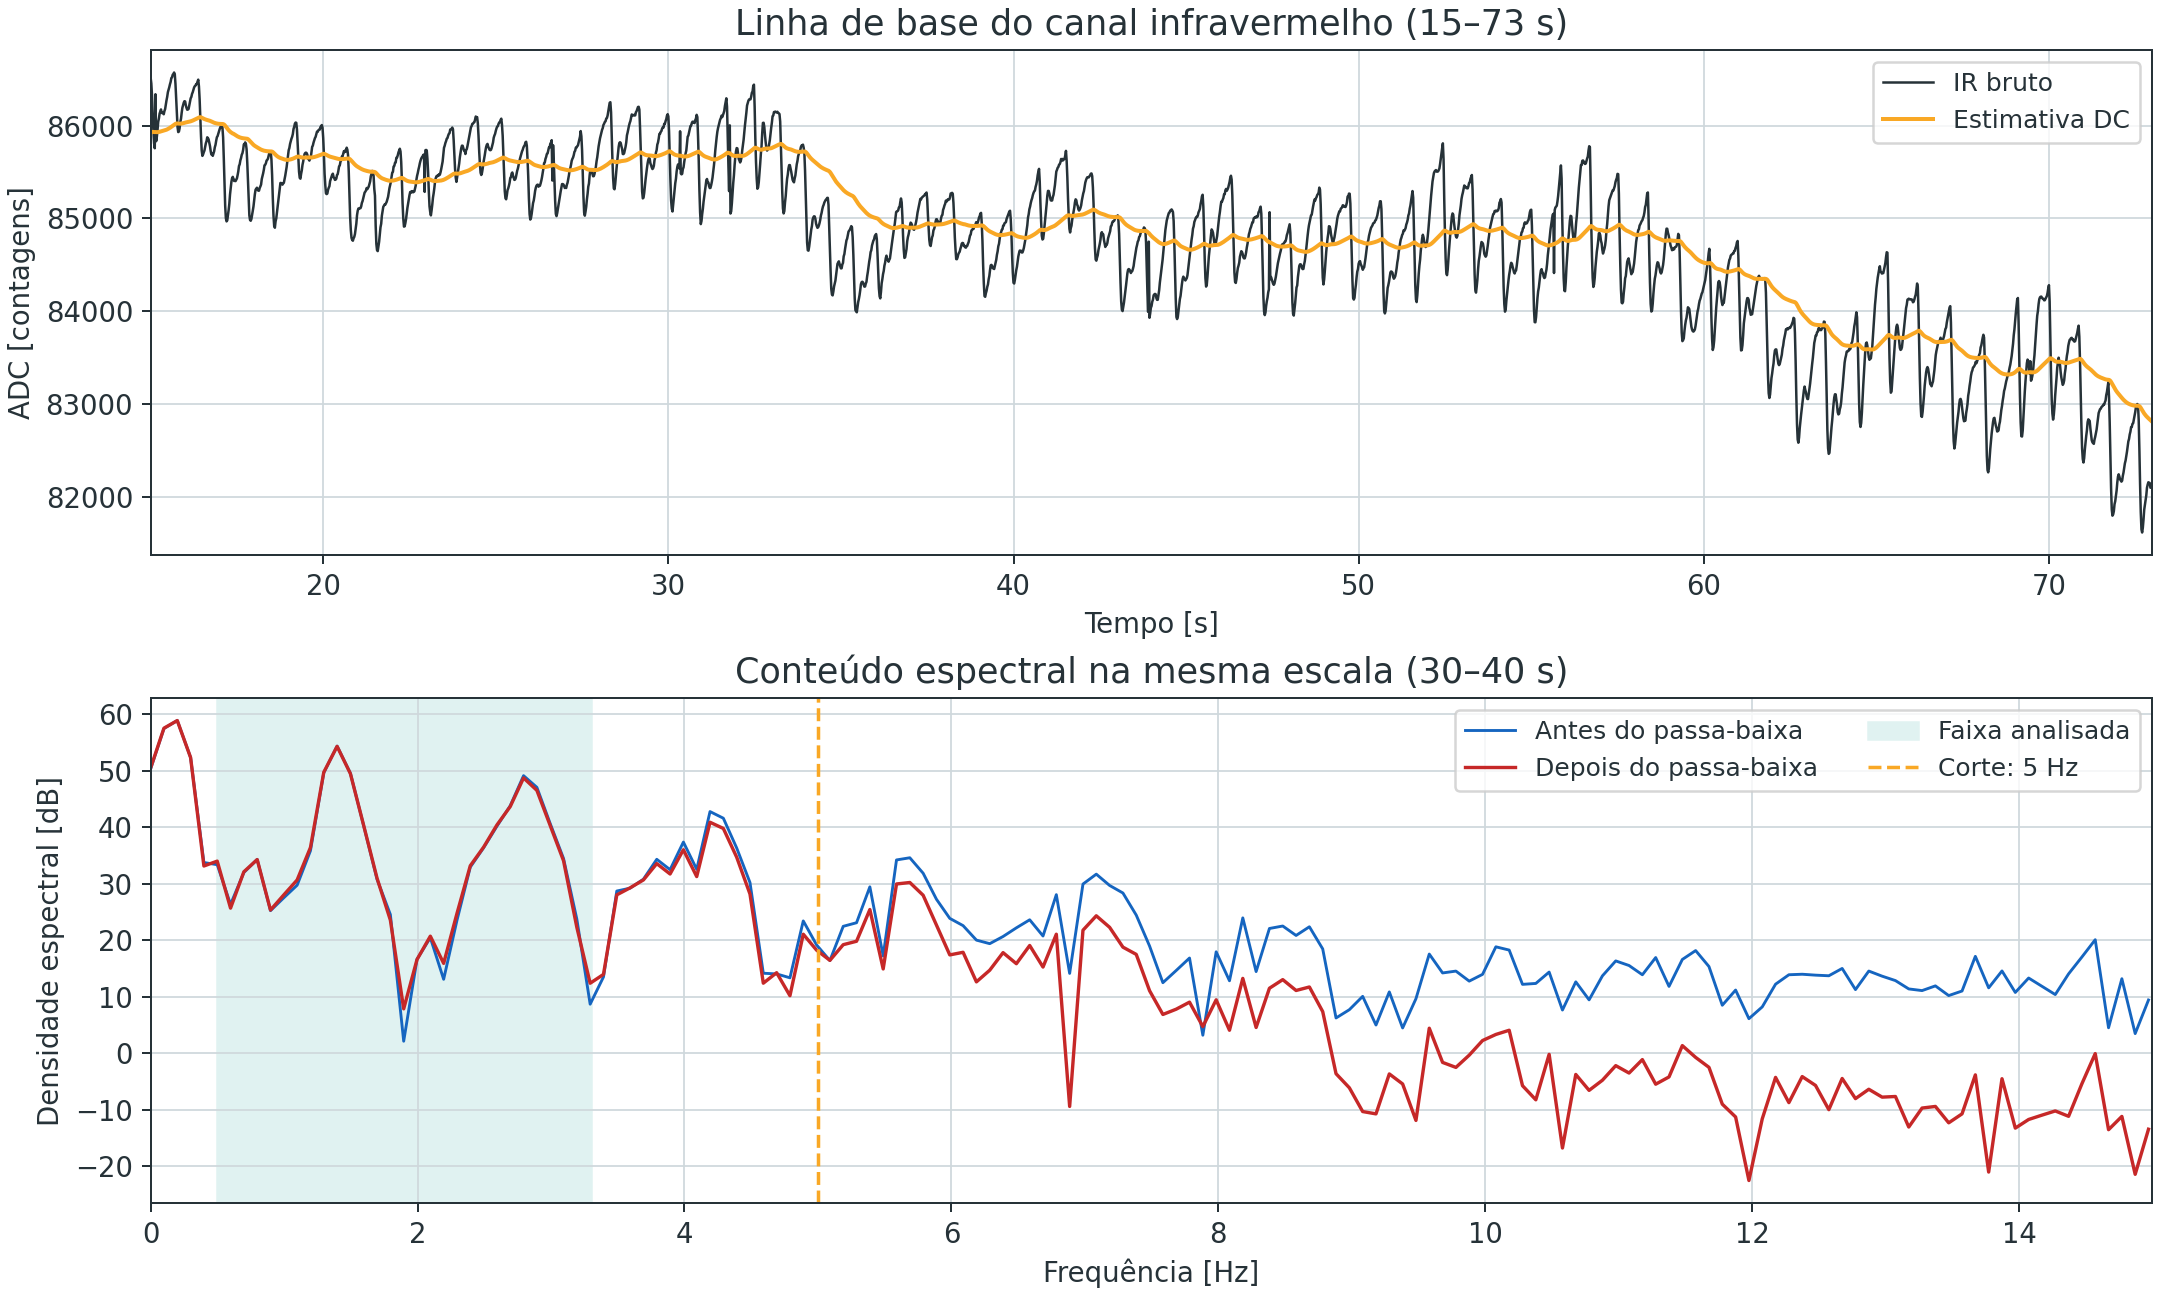
\includegraphics[width=0.98\textwidth]{Diagramas/max30102/max30102_ppg_condicionamento_15_73s.png}
\fonteelemento{Elaborado pelo autor a partir do CSV do ensaio standalone}
\end{figure}

O painel superior mostra a estimativa DC acompanhando a linha de base dominante do canal IR. O painel inferior confirma que a resposta antes e depois do passa-baixa permanece semelhante na faixa analisada e se separa progressivamente acima do corte de 5 Hz. N\~ao foi calculada rela\c{c}\~ao sinal-ru\'ido porque n\~ao havia trecho rotulado contendo somente ru\'ido sob a mesma condi\c{c}\~ao de contato. Tamb\'em n\~ao foi executada uma abla\c{c}\~ao do detector de batimentos com e sem o passa-baixa. Assim, os dados sustentam estima\c{c}\~ao de linha de base e limita\c{c}\~ao de banda, mas n\~ao demonstram que o passa-baixa tenha melhorado a exatid\~ao da frequ\^encia card\'iaca ou da SpO$_2$.


\subsubsection{Frequ\^encia card\'iaca e estimativa de SpO$_2$}

O teste standalone foi executado durante aproximadamente 65 s, com o ox\'imetro de dedo ECH e o Amazfit Active 2 operando simultaneamente. O ox\'imetro foi adotado como comparador principal. No primeiro trecho, ambos indicaram 81 BPM. Nas mudan\c{c}as seguintes, o MAX30102 acompanhou a dire\c{c}\~ao das cinco varia\c{c}\~oes observadas, mas apresentou subestima\c{c}\~ao em torno de 5 BPM nos patamares superiores, valores transit\'orios de 62 e 86 BPM e intervalos em estado de c\'alculo.

A SpO$_2$ do ox\'imetro permaneceu em 97\%, enquanto o MAX30102 indicou 98\% a 99\%. A diferen\c{c}a de 1 a 2 pontos percentuais e a estabilidade da indica\c{c}\~ao s\~ao compat\'iveis com um teste de plausibilidade, mas n\~ao constituem valida\c{c}\~ao cl\'inica. O ensaio foi realizado com um participante, instrumento de consumo sem certificado de calibra\c{c}\~ao e configura\c{c}\~ao standalone distinta da integra\c{c}\~ao final. A Figura~\ref{fig:fc-comparacao} sintetiza as indica\c{c}\~oes de frequ\^encia card\'iaca.

\begin{figure}[H]
\centering
\caption{Frequ\^encia card\'iaca indicada pelo MAX30102 e faixa observada no ox\'imetro}
\label{fig:fc-comparacao}
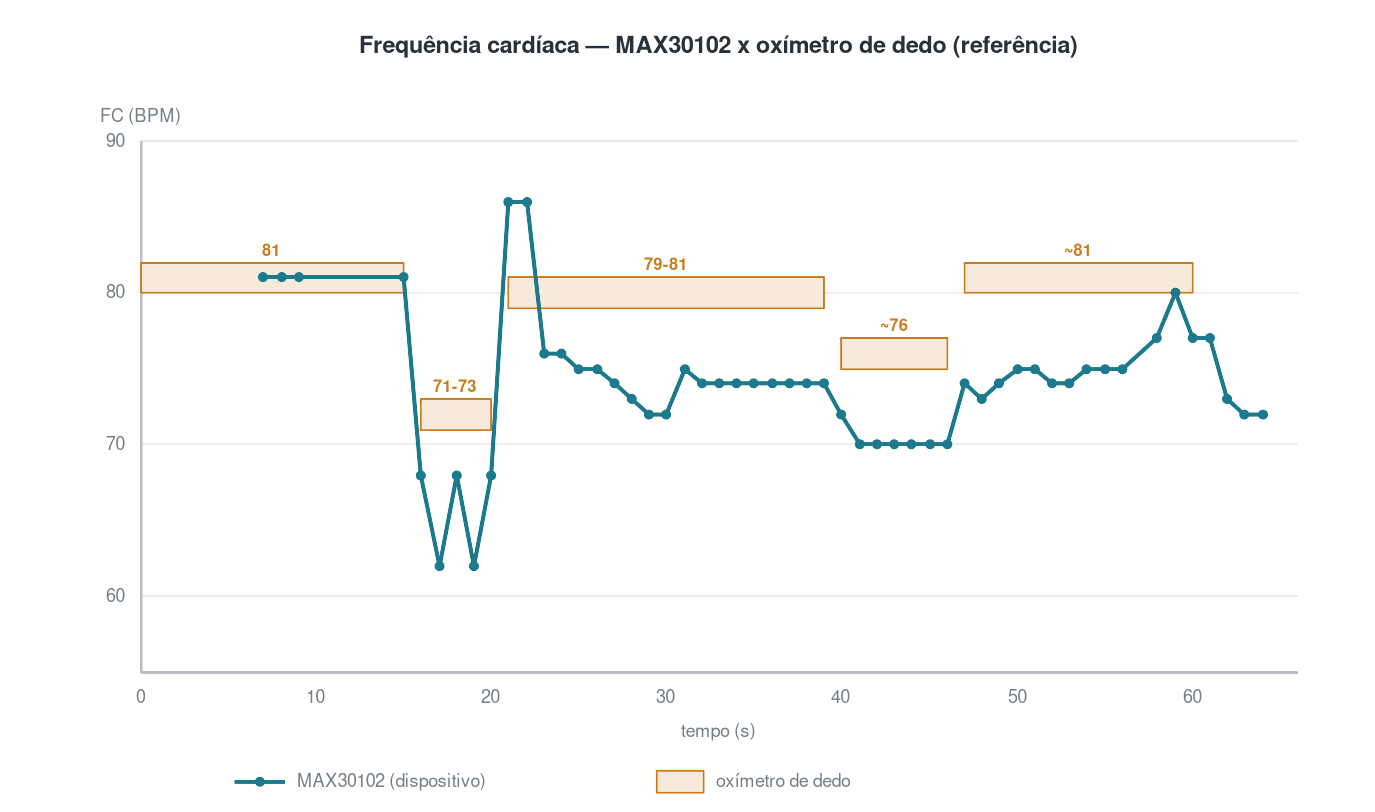
\includegraphics[width=0.95\textwidth]{Diagramas/max30102/max30102_fc_vs_referencia.png}
\fonteelemento{Elaborado pelo autor a partir do caderno de ensaios}
\end{figure}


A frequ\^encia card\'iaca e a SpO$_2$ permanecem resultados funcionais do pipeline. Movimento, contato, perfus\~ao, luz ambiente e posi\c{c}\~ao alteram a qualidade do PPG, e a calibra\c{c}\~ao emp\'irica empregada n\~ao transforma o prot\'otipo em instrumento cl\'inico.


\subsubsection{Evolu\c{c}\~ao das corre\c{c}\~oes}


A contribui\c{c}\~ao mais bem documentada do m\'odulo \'e a evolu\c{c}\~ao do processamento. A vers\~ao inicial produzia estimativas pr\'oximas de 70\%. A reorganiza\c{c}\~ao incluiu remo\c{c}\~ao de DC mais lenta, filtragem passa-baixa, detec\c{c}\~ao por batimento, per\'iodo refrat\'ario, raz\~ao calculada por ciclo e crit\'erios de qualidade.


Outro registro associa valores pr\'oximos de 28\% \`a troca dos canais vermelho e infravermelho em determinadas placas de conex\~ao; ap\'os corrigir a atribui\c{c}\~ao, foi observado valor pr\'oximo de 96\%. Essa observa\c{c}\~ao n\~ao deve ser generalizada ao MAX30102, mas evidencia a necessidade de conferir a ordem efetiva dos dados no m\'odulo utilizado.


As faixas de 70\%, 28\% e 95\%--99\% descrevem etapas de depura\c{c}\~ao, n\~ao um estudo comparativo. Como condi\c{c}\~oes e sinais correspondentes n\~ao est\~ao dispon\'iveis, elas n\~ao permitem separar o efeito individual de cada corre\c{c}\~ao.


\subsubsection{Limita\c{c}\~oes}


O per\'iodo refrat\'ario fixo de 400 ms imp\~oe limite te\'orico de 150 batimentos por minuto. O processamento n\~ao utiliza o aceler\^ometro para cancelar artefatos de movimento e emprega crit\'erios fixos de qualidade. A montagem em protoboard tamb\'em apresentou sensibilidade da alimenta\c{c}\~ao aos pulsos de corrente dos emissores.


\subsection{DS18B20}


\subsubsection{Estabilidade}

Durante aproximadamente 5 min, o DS18B20 permaneceu em 22,5 $^\circ$C e o termo-higr\^ometro MFL Embutir indicou 23,4 $^\circ$C. A diferen\c{c}a foi de $-0,9$ $^\circ$C. A toler\^ancia de $\pm0,5$ $^\circ$C informada para o DS18B20 n\~ao foi combinada a uma faixa do comparador, pois seu certificado e sua especifica\c{c}\~ao n\~ao estavam dispon\'iveis. Como a compara\c{c}\~ao ocorreu em um \`unico ponto, o resultado demonstra estabilidade de curto prazo e plausibilidade, n\~ao exatid\~ao metrol\'ogica. A figura anteriormente produzida com uma toler\^ancia ``t\'ipica'' assumida para o termo-higr\^ometro foi exclu\'ida desta vers\~ao.


\subsubsection{Resposta t\'ermica}

Partindo de 23 $^\circ$C, a leitura no freezer atingiu 13,4 $^\circ$C ap\'os 1 min e 3,3 $^\circ$C ap\'os 2 min. No aquecimento pr\'oximo \`a chama, a leitura atingiu 70 $^\circ$C em 30 s, quando o ensaio foi interrompido para preservar o probe. O intervalo observado foi de aproximadamente 67 $^\circ$C, sem travamento ou satura\c{c}\~ao. Como os est\'imulos n\~ao foram acompanhados por refer\^encia calibrada, os valores da Figura~\ref{fig:ds18b20-transientes} caracterizam resposta funcional e n\~ao acur\'acia din\^amica.

\begin{figure}[H]
\centering
\caption{Resposta do DS18B20 aos transientes de resfriamento e aquecimento}
\label{fig:ds18b20-transientes}
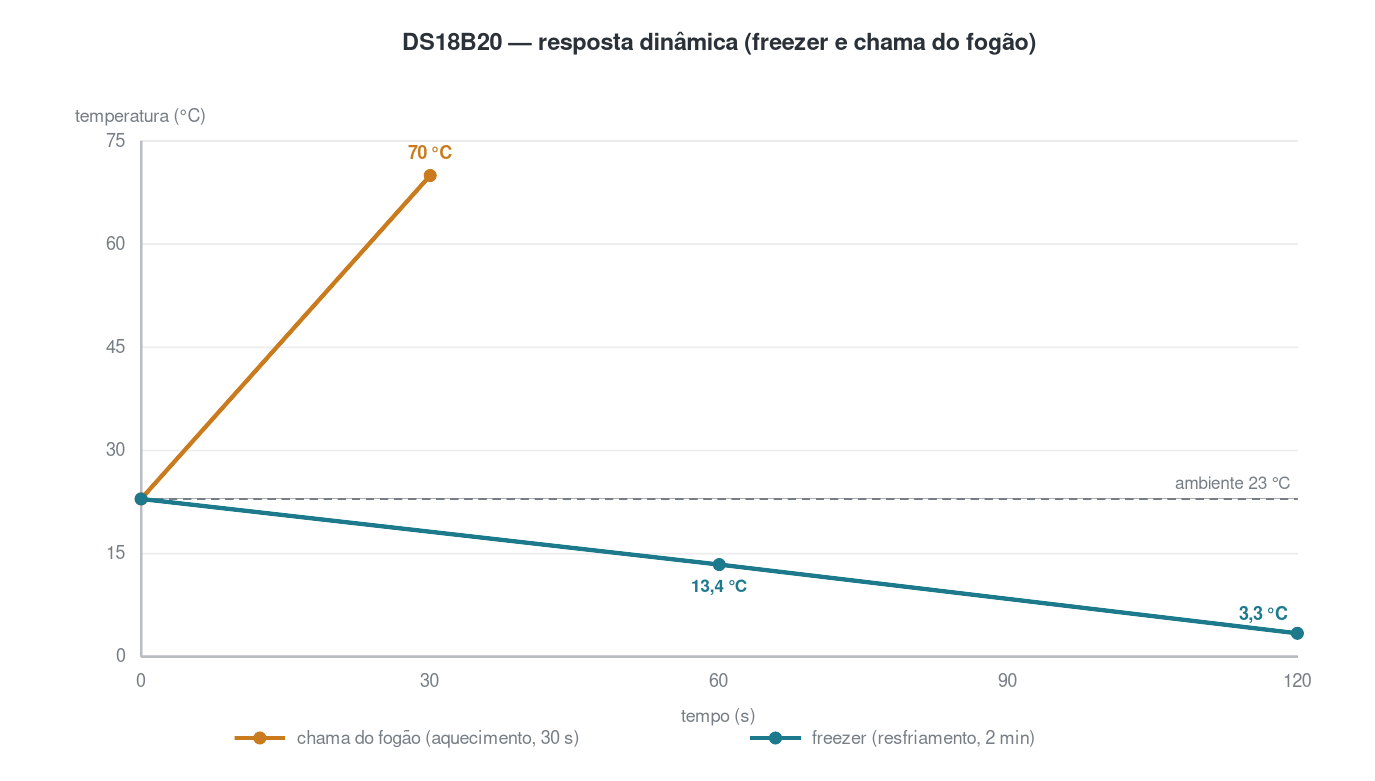
\includegraphics[width=0.85\textwidth]{Diagramas/ds18b20/ds18b20_resposta_dinamica.png}
\fonteelemento{Elaborado pelo autor a partir do caderno de ensaios}
\end{figure}


\subsubsection{Limita\c{c}\~oes}


A leitura depende da posi\c{c}\~ao, da transfer\^encia t\'ermica pela montagem e das fontes de calor pr\'oximas. Repeti\c{c}\~ao de um valor digital n\~ao deve ser interpretada como exatid\~ao.


\subsection{LTR390}


\subsubsection{Ambiente interno}


O compilado registra contagens entre 185 e 188 no canal ALS, correspondentes a aproximadamente 37,0--37,6 lux pela convers\~ao adotada. No mesmo ambiente, com ilumina\c{c}\~ao LED e janelas fechadas, o canal UVS permaneceu em zero.


A baixa varia\c{c}\~ao demonstra repetibilidade de curto prazo das contagens naquele cen\'ario, mas n\~ao exatid\~ao em lux. O valor nulo no canal UV \'e fisicamente plaus\'ivel em ambiente sem fonte ultravioleta relevante, embora n\~ao demonstre sensibilidade do canal a uma exposi\c{c}\~ao conhecida.


\subsubsection{Ensaio externo de UVI}


O resumo consolidado cita ensaio ao ar livre em Florian\'opolis no qual a estimativa variou entre UVI 3 e 6, com pico 6, enquanto uma refer\^encia meteorol\'ogica indicava UVI 5.


O registro indica resposta do sensor \`a radia\c{c}\~ao solar e compatibilidade de ordem de grandeza com a refer\^encia. N\~ao constitui calibra\c{c}\~ao, pois a refer\^encia meteorol\'ogica n\~ao foi medida junto ao sensor e pode representar intervalo espacial e temporal diferente.


O ensaio ocorreu em 25 de julho de 2026, em Florian\'opolis, sob c\'eu limpo. A aus\^encia de difusor cosseno e a movimenta\c{c}\~ao manual do prot\'otipo limitaram o controle angular. Em teste standalone adicional, uma lanterna UV gen\'erica elevou a indica\c{c}\~ao de 0 at\'e aproximadamente 4,0 conforme foi aproximada de 20 cm at\'e muito perto do sensor. Esse segundo ensaio confirma resposta qualitativa do canal, mas a fonte n\~ao caracterizada n\~ao fornece refer\^encia de UVI. A Figura~\ref{fig:ltr390-uvi} posiciona a faixa observada apenas para compara\c{c}\~ao qualitativa.

\begin{figure}[H]
\centering
\caption{Faixa de UVI indicada pelo LTR390 e valor meteorol\'ogico de refer\^encia}
\label{fig:ltr390-uvi}
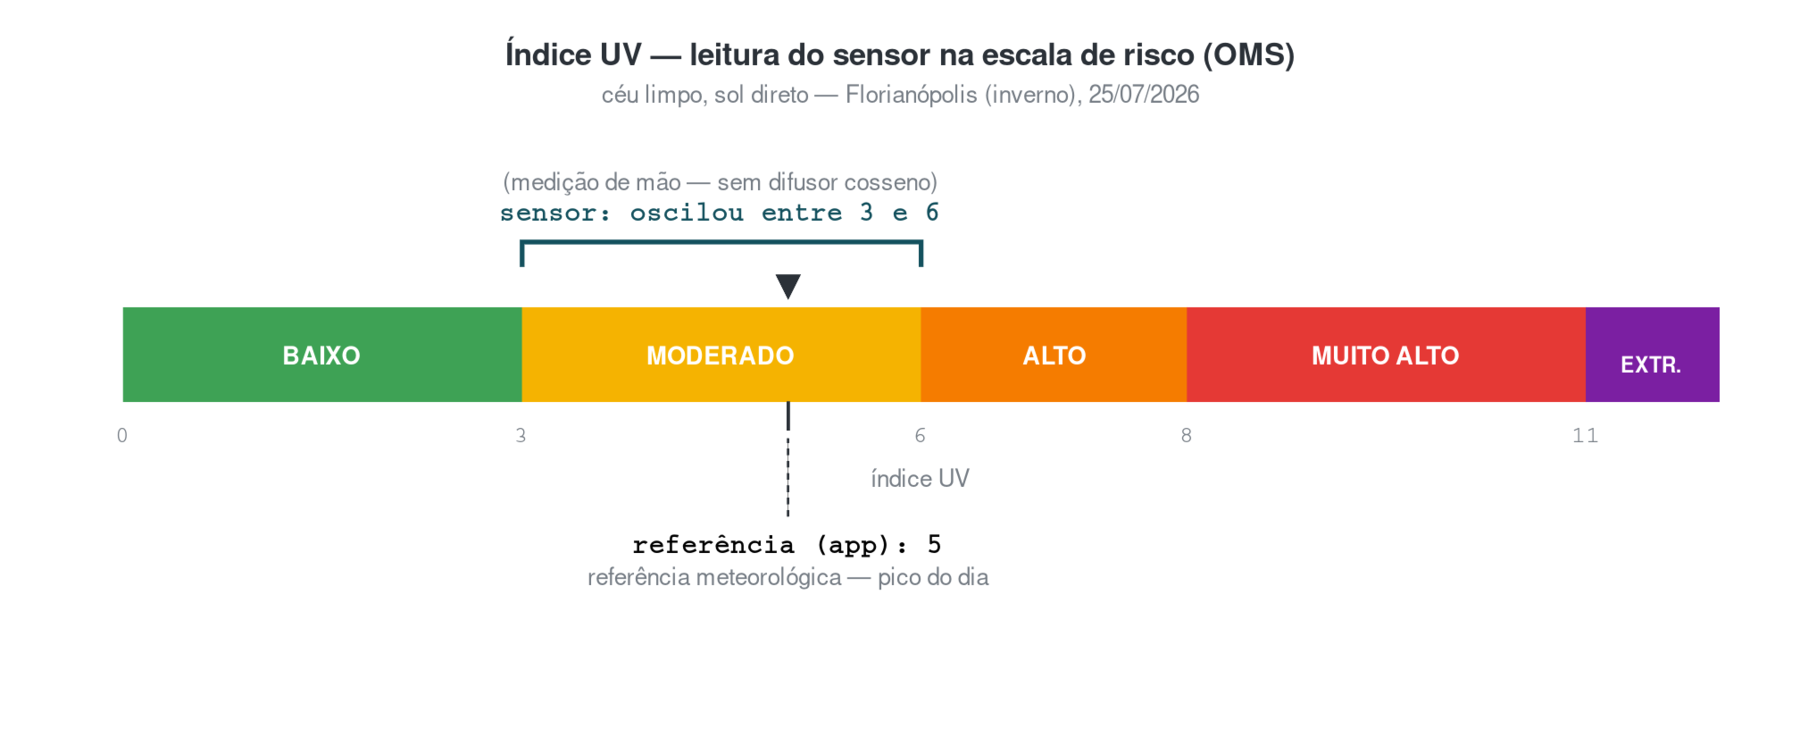
\includegraphics[width=0.8\textwidth]{Diagramas/ltr390/ltr390_uv_escala_risco.png}
\fonteelemento{Elaborado pelo autor a partir do caderno de ensaios e da refer\^encia meteorol\'ogica consultada}
\end{figure}


\subsubsection{Faixa e satura\c{c}\~ao de ilumin\^ancia}


O mesmo resumo informa resposta desde obstru\c{c}\~ao at\'e aproximadamente 52 klux e satura\c{c}\~ao pr\'oxima desse valor na configura\c{c}\~ao de ganho 3$\times$ e 18 bits. A satura\c{c}\~ao deve ser atribu\'ida \`a configura\c{c}\~ao usada, n\~ao ao limite absoluto do LTR390.


Foram observados 0 lux no escuro, aproximadamente 10--30 lux sob ilumina\c{c}\~ao urbana noturna, 100--150 lux em ambiente interno, cerca de 4000 lux em sombra externa e 51--52 klux sob sol direto. O \`ultimo valor coincide com o teto calculado de aproximadamente 52,4 klux para ganho 3$\times$ e resolu\c{c}\~ao de 18 bits, indicando satura\c{c}\~ao da configura\c{c}\~ao, n\~ao necessariamente da faixa absoluta do sensor. A Figura~\ref{fig:ltr390-lux} usa escala logar\'itmica para reunir essas ordens de grandeza.

\begin{figure}[H]
\centering
\caption{Ilumin\^ancia observada e teto da configura\c{c}\~ao utilizada}
\label{fig:ltr390-lux}
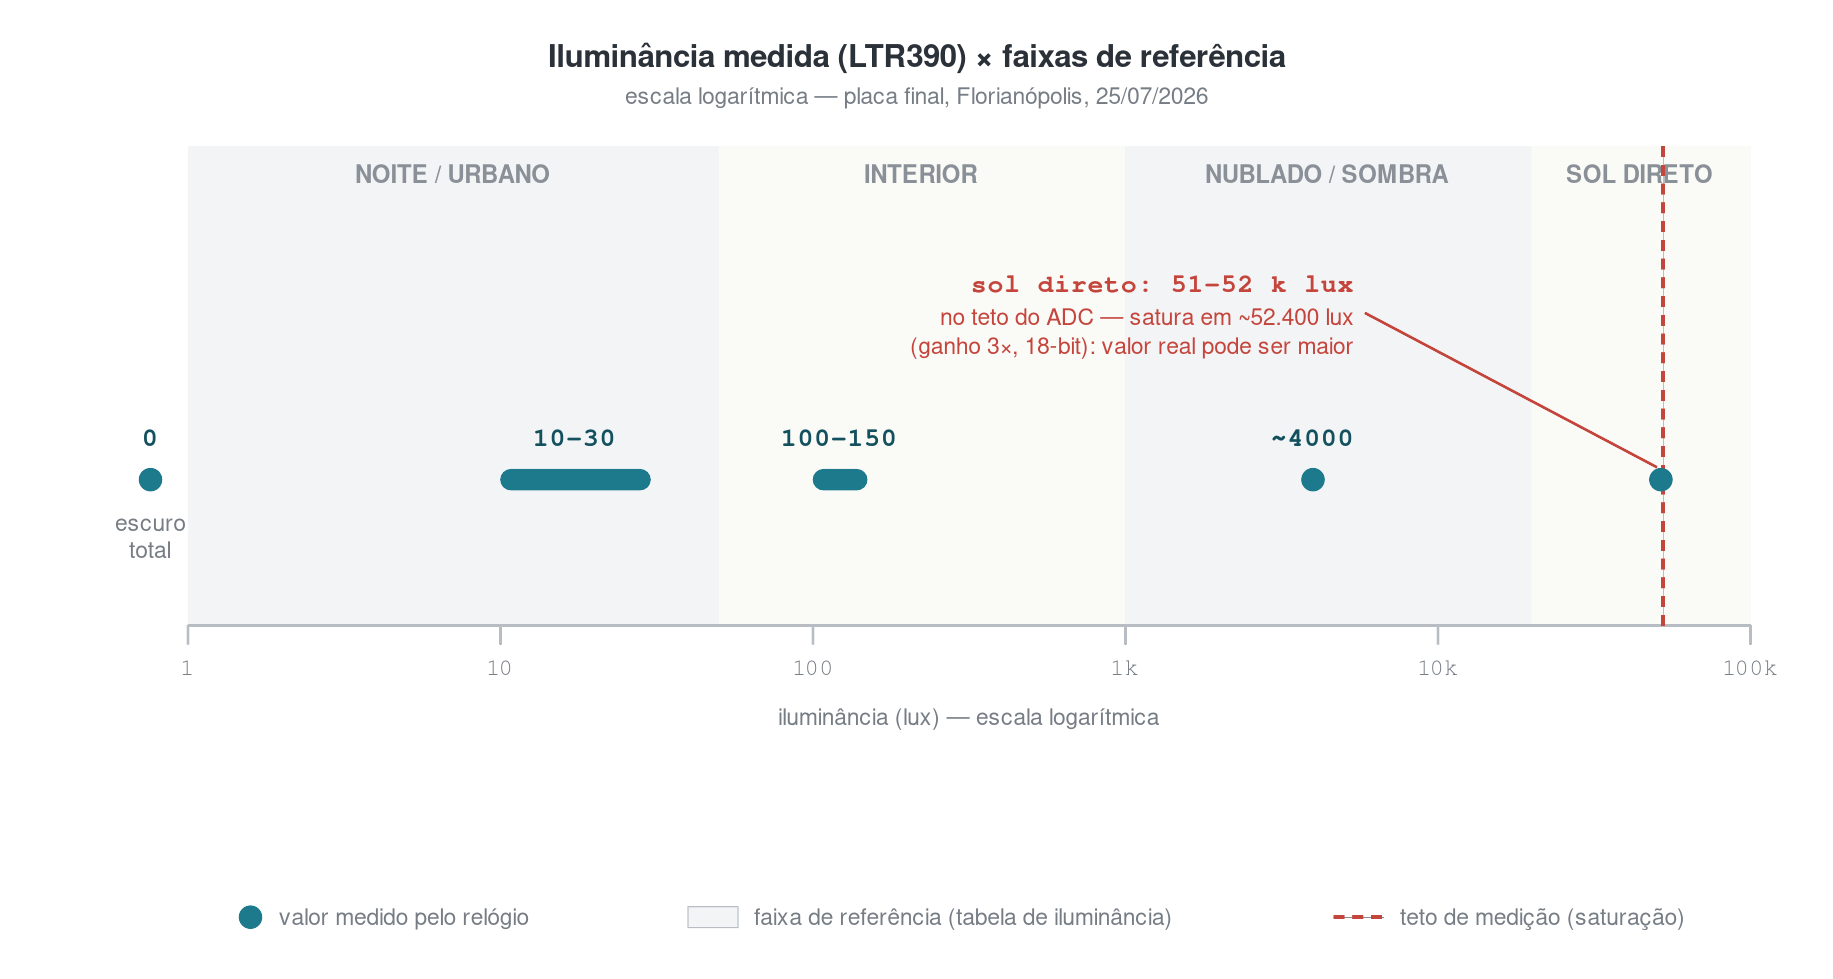
\includegraphics[width=0.85\textwidth]{Diagramas/ltr390/ltr390_lux_escala_log.png}
\fonteelemento{Elaborado pelo autor a partir do caderno de ensaios}
\end{figure}


\subsubsection{Limita\c{c}\~oes}


ALS e UVS n\~ao s\~ao medidos simultaneamente. A altern\^ancia introduz intervalo de estabiliza\c{c}\~ao e mant\'em cada valor at\'e a pr\'oxima ativa\c{c}\~ao do canal. Janela \'optica, orienta\c{c}\~ao, sombra e espectro da fonte afetam as leituras.


\subsection{B\'ussola}


\subsubsection{Calibra\c{c}\~ao}


A calibra\c{c}\~ao no pr\'oprio dispositivo, dividida em 12 setores e persistida em NVS, substituiu o fluxo anterior de exporta\c{c}\~ao CSV. A divis\~ao em setores orienta a coleta, mas a calibra\c{c}\~ao diagonal n\~ao corrige termos cruzados de \emph{soft iron}.


N\~ao foi preservada uma nuvem de pontos antes e depois da calibra\c{c}\~ao nem o conjunto final de par\^ametros usado no ensaio. Assim, a centraliza\c{c}\~ao, as diferen\c{c}\~as de escala e a cobertura tridimensional n\~ao foram quantificadas. A figura conceitual apresentada na Fundamenta\c{c}\~ao explica o m\'etodo, mas n\~ao foi reutilizada aqui como se fosse resultado do prot\'otipo.


\subsubsection{Heading}

Com o prot\'otipo e a b\'ussola Norvix DC45-2 nivelados no mesmo plano, foram comparadas duas orienta\c{c}\~oes na vers\~ao de ensaio, que n\~ao aplicava ajuste de declina\c{c}\~ao. Na ida, a Norvix indicou 320$^\circ$ e o prot\'otipo 336$^\circ$, diferen\c{c}a de +16$^\circ$. Na volta, as indica\c{c}\~oes foram 130$^\circ$ e 152$^\circ$, diferen\c{c}a de +22$^\circ$. A diferen\c{c}a m\'edia assinada foi +19$^\circ$.

Como ambos os instrumentos indicavam norte magn\'etico, o deslocamento n\~ao pode ser atribu\'ido \`a declina\c{c}\~ao. Calibra\c{c}\~ao residual, alinhamento visual, interfer\^encia da montagem e diferen\c{c}a entre os instrumentos s\~ao explica\c{c}\~oes poss\'iveis, mas n\~ao separadas pelo procedimento. O ensaio confirma resposta direcional, mas n\~ao sustenta alega\c{c}\~ao de precis\~ao. A Figura~\ref{fig:bussola-comparacao} identifica explicitamente a vers\~ao magn\'etica avaliada.


\begin{figure}[H]
\centering
\caption{Compara\c{c}\~ao magn\'etica entre o prot\'otipo e a b\'ussola de consumo}
\label{fig:bussola-comparacao}
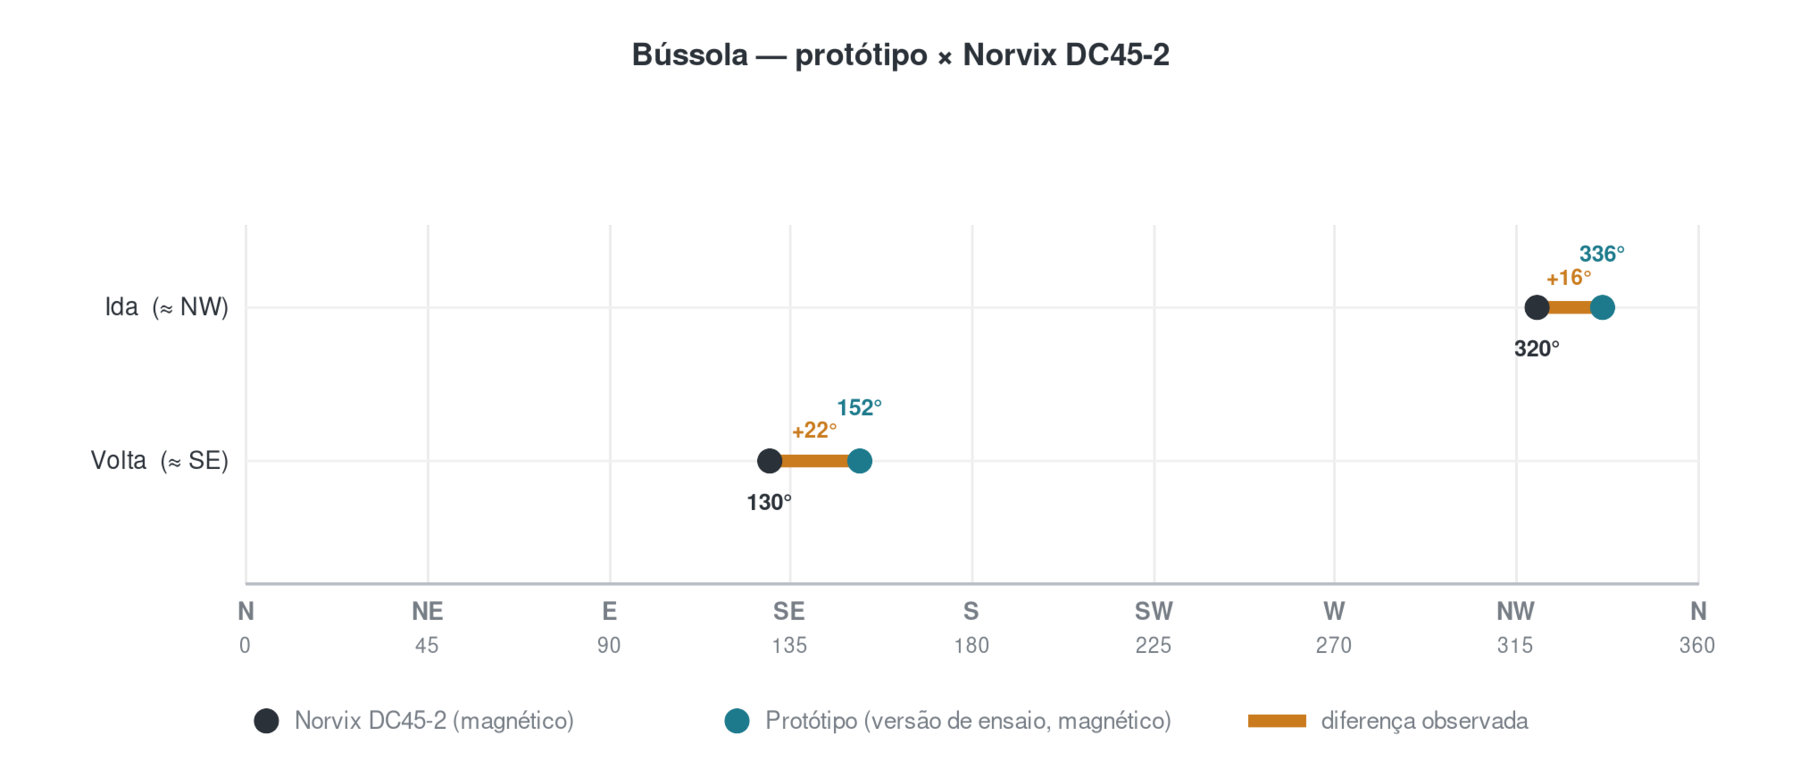
\includegraphics[width=0.95\textwidth]{Diagramas/mpu9250/mpu9250_bussola_declinacao.png}
\fonteelemento{Elaborado pelo autor a partir do caderno de ensaios}
\end{figure}


\subsubsection{Limita\c{c}\~oes}


Os valores do ensaio referem-se ao norte magn\'etico porque a vers\~ao avaliada n\~ao aplicava declina\c{c}\~ao. O firmware corrente acrescenta um valor fixo de $-21^\circ$; essa altera\c{c}\~ao posterior n\~ao deve ser usada para reinterpretar retroativamente as medidas. Inclina\c{c}\~ao do dispositivo projeta a componente vertical do campo nos eixos do c\'alculo, e a compensa\c{c}\~ao correspondente n\~ao foi implementada. Materiais ferromagn\'eticos e correntes do prot\'otipo podem alterar a calibra\c{c}\~ao.


\subsection{Ped\^ometro}


\subsubsection{Teste qualitativo}


O compilado descreve balan\c{c}o manual da protoboard e uma simula\c{c}\~ao com o sensor preso \`a perna. Foram relatadas detec\c{c}\~oes durante movimento, aus\^encia de falsos positivos em repouso e correspond\^encia considerada razo\'avel com os passos executados.


N\~ao foram informados n\'umero de passos, dura\c{c}\~ao do repouso, ritmo, posi\c{c}\~ao exata, repeti\c{c}\~oes nem erros. O registro confirma que o algoritmo responde a oscila\c{c}\~oes, mas n\~ao caracteriza seu desempenho como ped\^ometro.


\subsubsection{Ensaio controlado}

Em percurso de 100 m delimitado no Google Maps, a contagem manual foi de 140 passos tanto na ida quanto na volta. O prot\'otipo registrou 131 e 133 passos, correspondentes a erros de $-6,4$\% e $-5,0$\%, com m\'edia de $-5,7$\%. O Amazfit Active 2 registrou 175 e 167 passos, erros de +25,0\% e +19,3\%. A diferen\c{c}a entre as duas repeti\c{c}\~oes foi de 2 passos no prot\'otipo e 8 no comparador comercial. A Tabela~\ref{tab:pedometro-100m} organiza os valores observados.

\begin{table}[H]
\centering
\caption{Contagens e erros observados no percurso de 100 m}
\label{tab:pedometro-100m}
\begin{tabular}{lrrrrr}
\toprule
Percurso & Manual & Prot\'otipo & Erro (\%) & Amazfit & Erro (\%) \\
\midrule
Ida   & 140 & 131 & $-6,4$ & 175 & $+25,0$ \\
Volta & 140 & 133 & $-5,0$ & 167 & $+19,3$ \\
\bottomrule
\end{tabular}
\fonteelemento{Elaborado pelo autor a partir do caderno de ensaios}
\end{table}

O resultado indica subestima\c{c}\~ao moderada e pequena varia\c{c}\~ao entre os dois percursos nas condi\c{c}\~oes observadas. Entretanto, limita-se a um participante, um ritmo e duas repeti\c{c}\~oes. A dist\^ancia m\'edia por passo calculada pela refer\^encia foi 0,714 m, pr\'oxima do valor fixo de 0,70 m empregado pelo firmware. A Figura~\ref{fig:pedometro-ensaio} preserva as contagens de cada percurso.

\begin{figure}[H]
\centering
\caption{Contagem manual, prot\'otipo e Amazfit Active 2 no percurso de 100 m}
\label{fig:pedometro-ensaio}
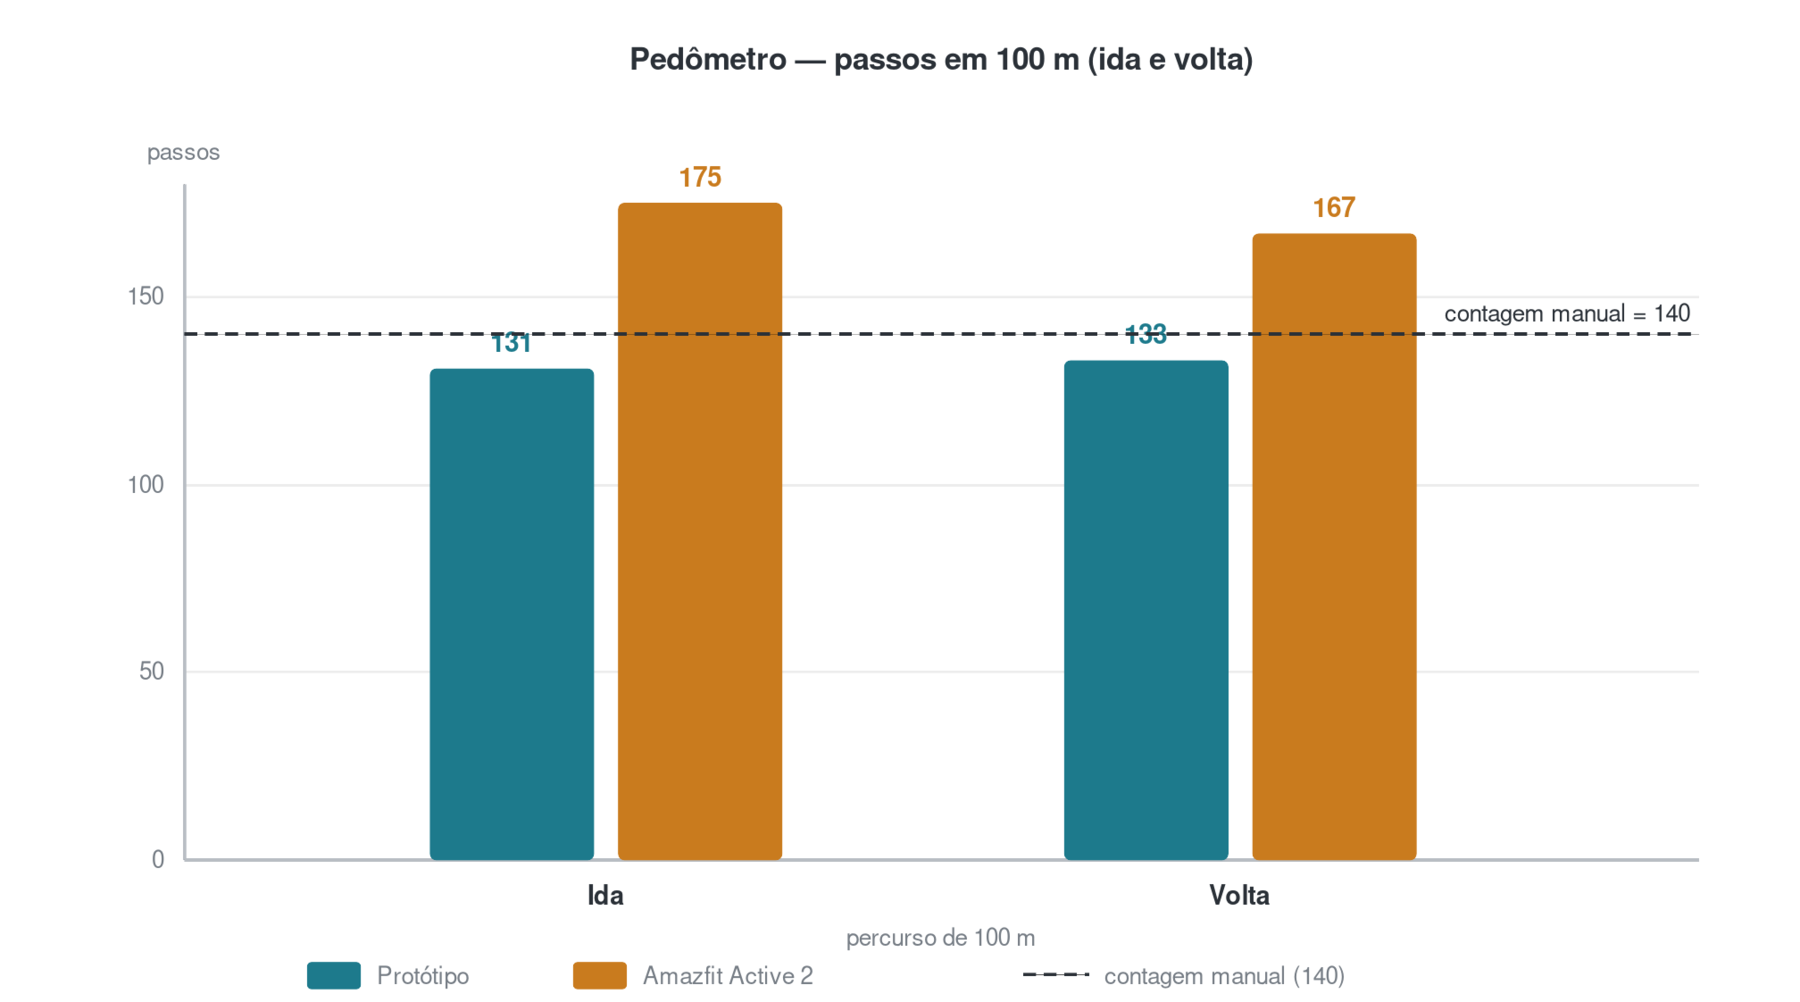
\includegraphics[width=0.85\textwidth]{Diagramas/mpu9250/mpu9250_pedometro_passos.png}
\fonteelemento{Elaborado pelo autor a partir do caderno de ensaios}
\end{figure}


\subsubsection{Limita\c{c}\~oes}


Limiar, histerese e intervalo m\'inimo s\~ao fixos. Movimentos do bra\c{c}o ou do dispositivo podem produzir cruzamentos semelhantes aos da marcha, enquanto passos suaves podem n\~ao atingir o limiar. A dist\^ancia usa comprimento fixo de 0,70 m e n\~ao foi individualizada. O contador retorna a zero ap\'os reinicializa\c{c}\~ao.


\subsection{Interface gr\'afica}


Os compilados registram funcionamento da exibi\c{c}\~ao de hora e data, anel de segundos, edi\c{c}\~ao por toque, grava\c{c}\~ao no PCF8563 e navega\c{c}\~ao entre as fun\c{c}\~oes. A calibra\c{c}\~ao da b\'ussola e o in\'icio da aquisi\c{c}\~ao PPG tamb\'em utilizam controles gr\'aficos.


A identifica\c{c}\~ao do CHSC6X por varredura em 0x2E permitiu substituir o driver inicialmente escolhido com base na documenta\c{c}\~ao de outra revis\~ao. A fonte restrita a 11 glifos reduziu armazenamento e exigiu que o feedback da edi\c{c}\~ao fosse implementado por opacidade.


Esses resultados demonstram integra\c{c}\~ao funcional entre toque, RTC, LVGL e m\'odulos. As capturas da Figura~\ref{fig:interface-final} pertencem \`a mesma sequ\^encia registrada no firmware corrente e documentam a tela principal, as quatro p\'aginas de menu por meio de exemplos representativos e telas funcionais.


\begin{figure}[H]
\centering
\caption{Capturas da interface execut\'avel da plataforma}
\label{fig:interface-final}
\begin{subfigure}[t]{0.26\textwidth}
\centering
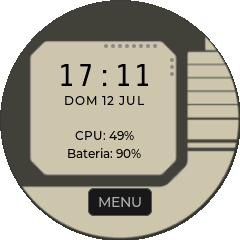
\includegraphics[width=\linewidth]{Telas Display/tela_230002_01_MenuPrincipal.png}
\caption{Tela principal}
\end{subfigure}
\hfill
\begin{subfigure}[t]{0.26\textwidth}
\centering
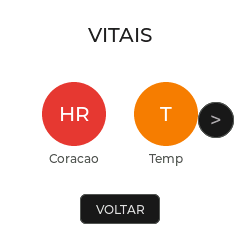
\includegraphics[width=\linewidth]{Telas Display/tela_230024_02_VitaisMenu.png}
\caption{Sinais vitais}
\end{subfigure}
\hfill
\begin{subfigure}[t]{0.26\textwidth}
\centering
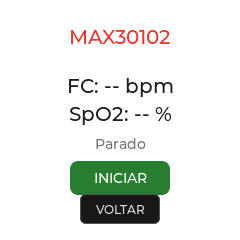
\includegraphics[width=\linewidth]{Telas Display/tela_230056_03_MaxScreen.png}
\caption{PPG}
\end{subfigure}

\medskip
\begin{subfigure}[t]{0.26\textwidth}
\centering
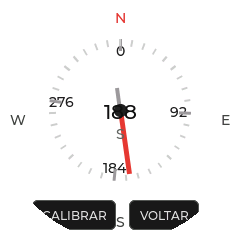
\includegraphics[width=\linewidth]{Telas Display/tela_230333_09_CompScreen.png}
\caption{B\'ussola}
\end{subfigure}
\hfill
\begin{subfigure}[t]{0.26\textwidth}
\centering
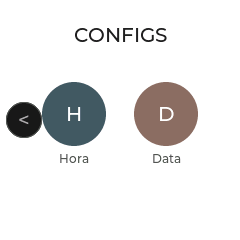
\includegraphics[width=\linewidth]{Telas Display/tela_230412_11_ConfigMenu.png}
\caption{Configura\c{c}\~oes}
\end{subfigure}
\hfill
\begin{subfigure}[t]{0.26\textwidth}
\centering
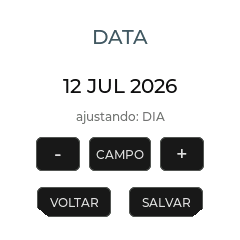
\includegraphics[width=\linewidth]{Telas Display/tela_230505_13_DataScreen.png}
\caption{Ajuste de data}
\end{subfigure}
\begin{minipage}{0.92\textwidth}
\fonteelemento{Capturas do firmware integrado produzidas pelo autor}
\end{minipage}
\end{figure}

No ensaio do RTC, a hora foi ajustada na troca de minuto da refer\^encia oficial de Bras\'ilia. Depois de 1 h com o sistema ligado, n\~ao foi observado desvio na resolu\c{c}\~ao do procedimento. Em seguida, o sistema permaneceu desligado por 24 h; ao religar, o PCF8563 apresentou atraso de aproximadamente 2 s. O resultado demonstra que a bateria CR927 preservou a contagem durante o desligamento. A observa\c{c}\~ao de um \`unico intervalo de 24 h corresponde a cerca de 2 s/dia ou 23 ppm, mas n\~ao substitui caracteriza\c{c}\~ao de deriva por v\'arios dias. A sequ\^encia \'e sintetizada na Figura~\ref{fig:rtc-sequencia}.

\begin{figure}[H]
\centering
\caption{Sequ\^encia do ensaio de manuten\c{c}\~ao da hora com o sistema desligado}
\label{fig:rtc-sequencia}
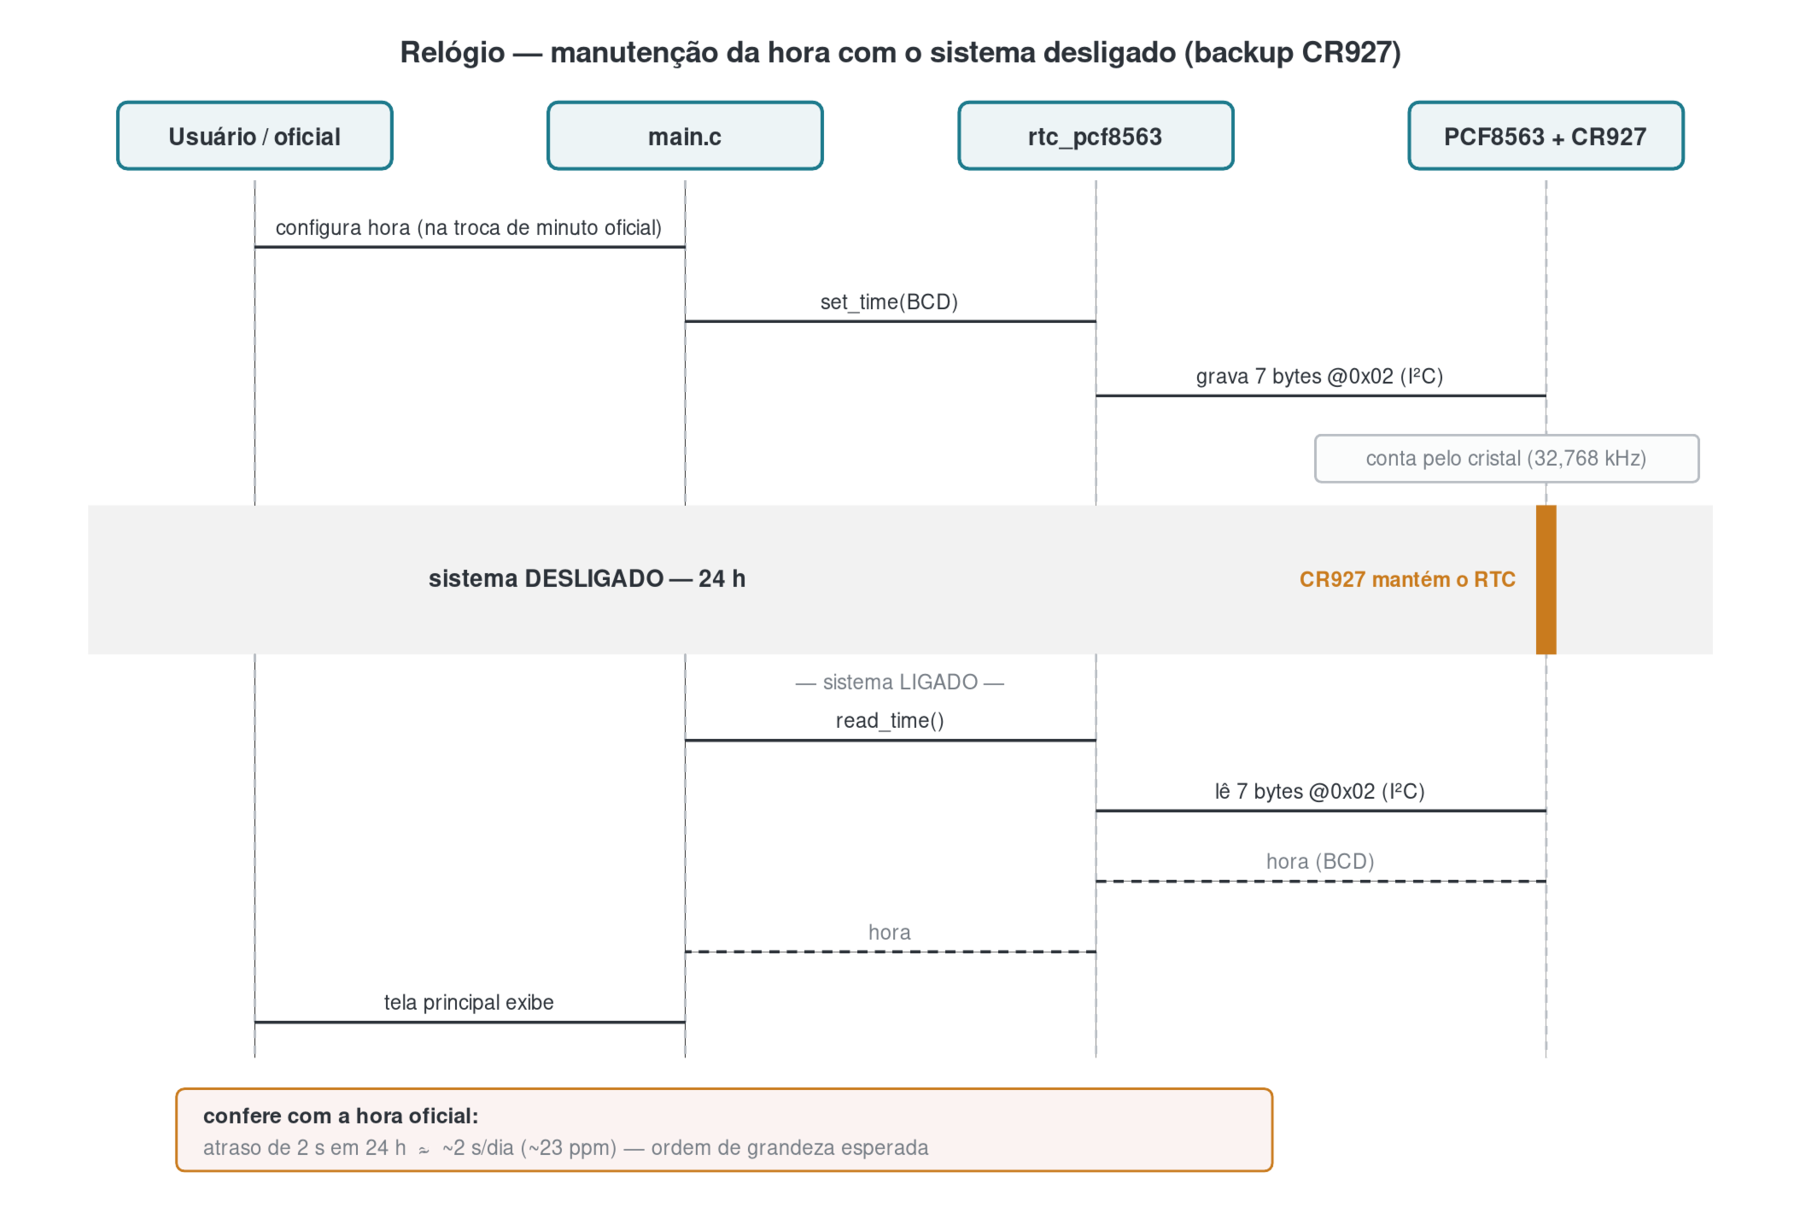
\includegraphics[width=0.95\textwidth]{Diagramas/round_display/relogio_rtc_sequencia.png}
\fonteelemento{Elaborado pelo autor a partir do caderno de ensaios}
\end{figure}


As capturas confirmam composi\c{c}\~ao e navegabilidade das telas mostradas, mas n\~ao medem lat\^encia nem taxa de falhas de toque. Essas m\'etricas n\~ao foram coletadas.


\subsection{Alimenta\c{c}\~ao e bateria}


O resumo consolidado registra leituras pontuais de aproximadamente 4,04 V com USB conectado e 3,84 V somente com bateria, associadas pelo firmware a 88\% e 56\%. Com USB, a tens\~ao observada pertence ao estado de carga e n\~ao representa a curva de descarga da c\'elula.


Essas leituras n\~ao sustentam autonomia, capacidade efetiva ou estado de carga com a exatid\~ao indicada pelos percentuais. O backlight permanece ligado e o gerenciamento avan\c{c}ado de energia n\~ao foi implementado.

O mult\'imetro foi ligado em s\'erie com a bateria para medir nove cen\'arios. A tela principal consumiu 110 mA; menu, 120 mA; temperatura, 150 mA; luz/UV, 130 mA; b\'ussola, 180 mA; calibra\c{c}\~ao da b\'ussola, 130 mA; ped\^ometro, 120 mA; tela PPG parada, 90 mA; e PPG medindo, 210 mA. As associa\c{c}\~oes entre essas diferen\c{c}as e atividades espec\'ificas de CPU, interface ou sensores s\~ao hip\'oteses a confirmar, pois o ensaio mediu somente a corrente total.

N\~ao foi executada descarga completa. Com capacidade \`util assumida de aproximadamente 1000 mAh, a raz\~ao entre capacidade e corrente fornece estimativas de autonomia dependentes do cen\'ario; elas n\~ao constituem autonomia medida. O backlight permaneceu ligado e os modos de baixo consumo foram tratados como proje\c{c}\~ao de trabalho futuro. A Figura~\ref{fig:consumo-cenarios} apresenta apenas as correntes totais observadas.

\begin{figure}[H]
\centering
\caption{Corrente total medida nos cen\'arios funcionais da plataforma}
\label{fig:consumo-cenarios}
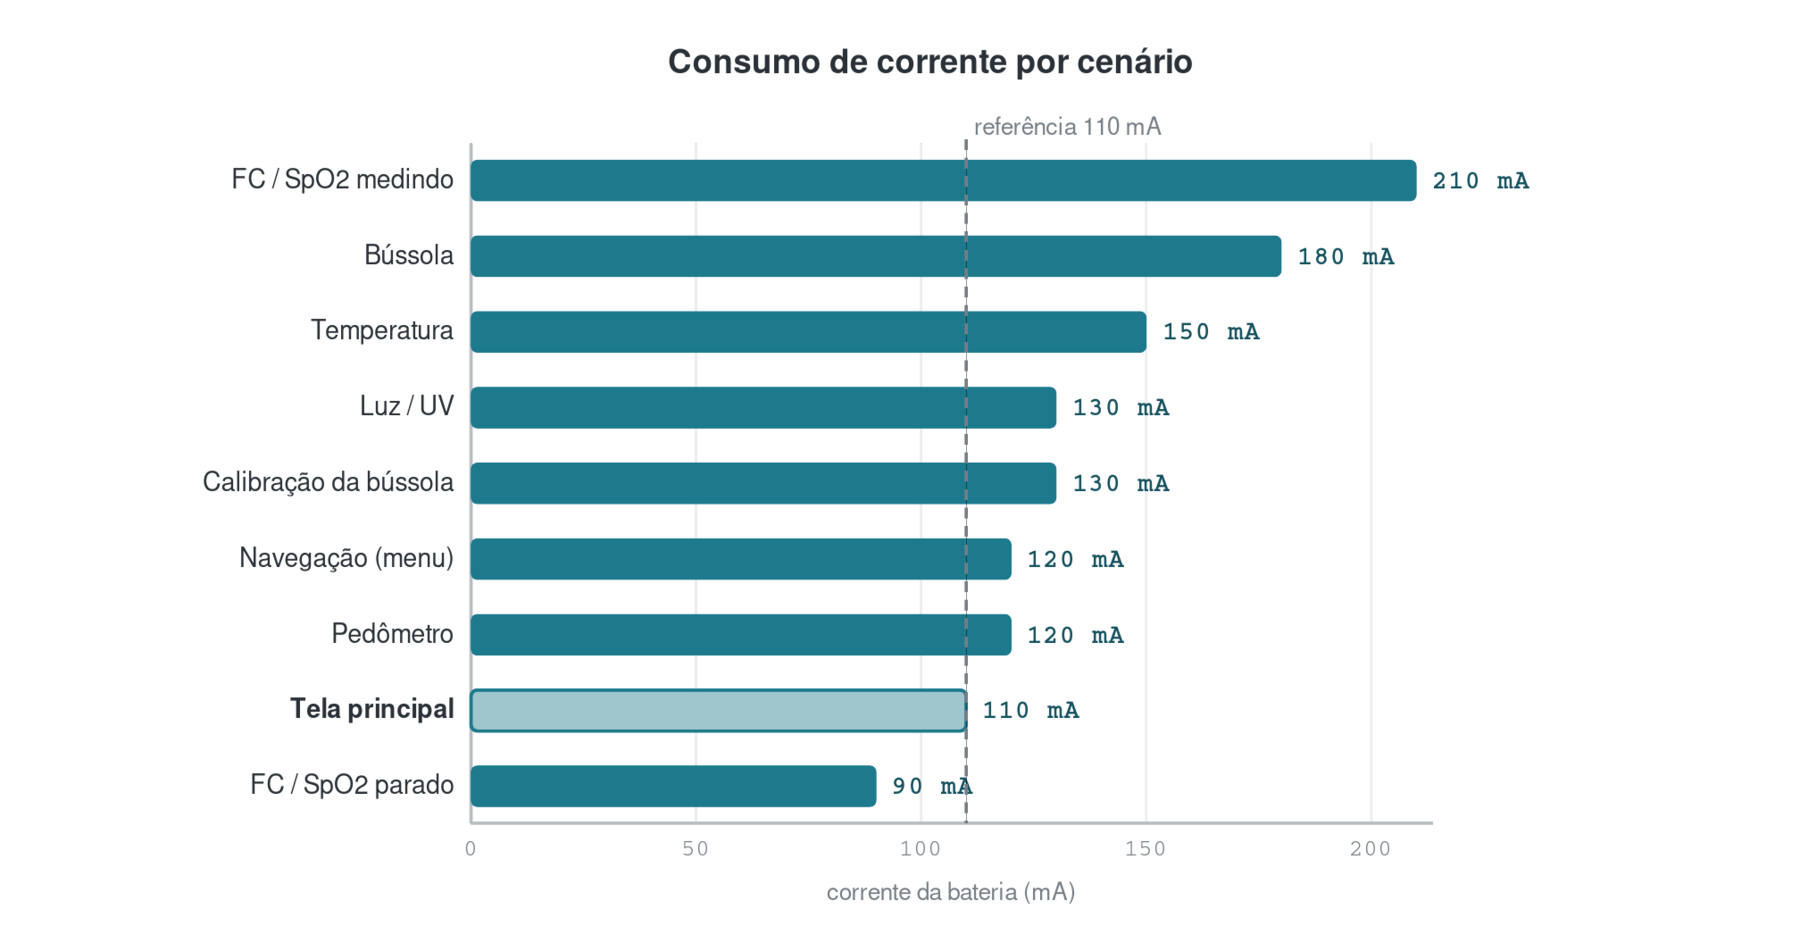
\includegraphics[width=0.85\textwidth]{Diagramas/bateria/bateria_consumo_por_cenario.png}
\fonteelemento{Elaborado pelo autor a partir do caderno de ensaios}
\end{figure}


\subsection{Discuss\~ao integrada}


A integra\c{c}\~ao funcional \'e a evid\^encia mais consistente do estado atual. O mesmo n\'ucleo organiza interface, RTC e quatro unidades sensoriais, apesar de diferen\c{c}as de transporte, per\'iodo e processamento. O contrato de m\'odulos, o registro de telas e as tarefas independentes materializam as caracter\'isticas de modularidade e extensibilidade descritas no projeto.


O barramento I$^2$C concentrou os principais efeitos sist\^emicos. \emph{Polling} excessivo do toque, NACK do LTR390 durante reset e verbosidade dos logs deixaram de ser problemas confinados aos respectivos drivers porque disputavam controlador, CPU e tempo de execu\c{c}\~ao. As corre\c{c}\~oes --- interrup\c{c}\~ao do toque, remo\c{c}\~ao do reset desnecess\'ario, mutex e recupera\c{c}\~ao --- mostram que a robustez depende da coordena\c{c}\~ao dos servi\c{c}os compartilhados.


Os ensaios com sensores ausentes complementam a an\'alise estrutural: a remo\c{c}\~ao individual de cada sensor e os diferentes arranjos de remo\c{c}\~ao n\~ao impediram a opera\c{c}\~ao do sistema principal nem dos m\'odulos independentes. Como a falha din\^amica do barramento n\~ao foi induzida e n\~ao se estabeleceu um protocolo estat\'istico de repeti\c{c}\~oes, essa rela\c{c}\~ao comprova a conten\c{c}\~ao funcional nas condi\c{c}\~oes testadas, mas n\~ao define uma taxa de confiabilidade.


Nos m\'odulos sensoriais, as evid\^encias possuem car\'ater funcional. O PPG foi comparado com ox\'imetro de consumo sem valida\c{c}\~ao cl\'inica; o DS18B20 foi comparado em um ponto com refer\^encia n\~ao calibrada; a compara\c{c}\~ao meteorol\'ogica do LTR390 n\~ao \'e calibra\c{c}\~ao; a b\'ussola apresentou diferen\c{c}as de 16$^\circ$ e 22$^\circ$ em apenas duas orienta\c{c}\~oes; e o ped\^ometro foi ensaiado com um participante, um ritmo e duas repeti\c{c}\~oes. Essa delimita\c{c}\~ao evita converter plausibilidade em valida\c{c}\~ao.


\subsection{Compara\c{c}\~ao com trabalhos relacionados}


O Amulet avalia uma plataforma para m\'ultiplas aplica\c{c}\~oes com \^enfase em energia, isolamento e acesso a recursos (HESTER et al., 2016). A WMP concentra-se na aquisi\c{c}\~ao sincronizada de sinais fisiol\'ogicos e em processamento remoto (BALDINI et al., 2023). O WEARDA prioriza coleta aberta e reprodut\'ivel de dados em um smartwatch comercial (VAN DIJK; GAWEHNS; VAN LEEUWEN, 2023).


O presente trabalho concentra-se no firmware de uma plataforma vest\'ivel modular multissensor constru\'ida sobre microcontrolador e sensores heterog\^eneos. Seu diferencial proposto est\'a no contrato de m\'odulos, na coordena\c{c}\~ao expl\'icita do I$^2$C compartilhado e na continuidade das fun\c{c}\~oes independentes quando um sensor est\'a ausente. Amulet e WMP apresentam avalia\c{c}\~oes experimentais mais estruturadas em seus respectivos objetivos.


A compara\c{c}\~ao n\~ao estabelece superioridade geral. Cada plataforma adota escopo, hardware e unidade de an\'alise diferentes, e as m\'etricas dispon\'iveis n\~ao permitem uma classifica\c{c}\~ao \'unica.


\subsection{Limita\c{c}\~oes gerais}


A placa prot\'otipo e o inv\'olucro impresso em 3D foram realizados, mas n\~ao passaram por caracteriza\c{c}\~ao mec\^anica, ambiental ou de uso prolongado. O backlight sempre ligado e a aus\^encia de gerenciamento avan\c{c}ado de energia limitam a autonomia; como n\~ao houve descarga completa, somente estimativas derivadas do consumo medido podem ser apresentadas.


N\~ao houve valida\c{c}\~ao cl\'inica do MAX30102, calibra\c{c}\~ao metrol\'ogica do LTR390, caracteriza\c{c}\~ao t\'ermica com refer\^encia rastre\'avel, compensa\c{c}\~ao de inclina\c{c}\~ao da b\'ussola nem caracteriza\c{c}\~ao estat\'istica do ped\^ometro para diferentes usu\'arios e ritmos.


Tamb\'em permaneceram fora do escopo a carga de CPU e o heap por cen\'ario, a mem\'oria incremental por m\'odulo, uma s\'erie controlada de tempo de boot, a recupera\c{c}\~ao I$^2$C sob falhas induzidas e um ensaio prolongado com navega\c{c}\~ao repet\'ivel.

\clearpage
\section{Conclus\~oes}


Este trabalho desenvolveu uma plataforma vest\'ivel modular multissensor baseada no XIAO ESP32-C6, no ESP-IDF e no FreeRTOS. O problema tratado foi a integra\c{c}\~ao de sensores heterog\^eneos, interface gr\'afica e servi\c{c}os compartilhados sem concentrar o processamento no n\'ucleo e sem interromper deliberadamente as fun\c{c}\~oes independentes quando um sensor n\~ao est\'a dispon\'ivel.


\subsection{Atendimento aos objetivos}


A vers\~ao implementada separa n\'ucleo, servi\c{c}os, drivers, processamento e telas. MAX30102, DS18B20, LTR390, b\'ussola e ped\^ometro seguem o ciclo comum de inicializa\c{c}\~ao, cria\c{c}\~ao e exibi\c{c}\~ao de tela, respeitadas as diferen\c{c}as de transporte. O despacho gr\'afico atua sobre a tela ativa, enquanto tarefas pr\'oprias executam as aquisi\c{c}\~oes. A navega\c{c}\~ao, as quatro p\'aginas de menu, o RTC e as telas funcionais foram confirmados pelo firmware e pelas capturas da interface.


O barramento I$^2$C foi centralizado em um servi\c{c}o comum com mutex, heran\c{c}a de prioridade, limites de espera, varredura no boot e recupera\c{c}\~ao p\'os-NACK. A an\'alise est\'atica confirmou esses caminhos, e os ensaios com remo\c{c}\~ao individual e combinada dos sensores mostraram que a aus\^encia de um ou mais componentes n\~ao impediu o uso do sistema principal nem dos m\'odulos independentes. Como n\~ao foram induzidas falhas durante a opera\c{c}\~ao nem executadas repeti\c{c}\~oes sob um protocolo estat\'istico, a evid\^encia sustenta a presen\c{c}a dos mecanismos e comprova a conten\c{c}\~ao funcional nas condi\c{c}\~oes testadas, mas n\~ao uma taxa de recupera\c{c}\~ao ou confiabilidade.


A extensibilidade e o acoplamento foram avaliados estruturalmente. No estudo retrospectivo do MAX30102, seis arquivos de processamento, com 678 linhas, foram reutilizados sem altera\c{c}\~ao; a integra\c{c}\~ao exigiu seis pontos expl\'icitos fora da pasta do m\'odulo e n\~ao modificou os demais m\'odulos sensoriais. Esse resultado demonstra localiza\c{c}\~ao das altera\c{c}\~oes no caso estudado, mas n\~ao mede o tempo necess\'ario para integrar um componente arbitr\'ario.


A compila\c{c}\~ao limpa produziu uma imagem grav\'avel de 784.240 bytes, correspondente a 74,79\% da parti\c{c}\~ao de 1 MiB. O resultado confirma o enquadramento global do firmware integrado. N\~ao foram obtidos incrementos por m\'odulo nem medidas compar\'aveis de CPU e heap por cen\'ario, de modo que a caracteriza\c{c}\~ao de recursos permanece parcial.


\subsection{Contribui\c{c}\~oes e alcance dos resultados}


A contribui\c{c}\~ao principal \'e a organiza\c{c}\~ao concreta de uma plataforma multissensor em contratos e servi\c{c}os compartilhados. A implementa\c{c}\~ao concentra em cada m\'odulo o acesso ao dispositivo, o processamento, o estado e a apresenta\c{c}\~ao, enquanto o n\'ucleo coordena inicializa\c{c}\~ao, registro e navega\c{c}\~ao. A placa prot\'otipo autoral e o inv\'olucro impresso em 3D tamb\'em foram realizados e integram o resultado de implementa\c{c}\~ao.


Os ensaios sensoriais demonstraram funcionamento, n\~ao valida\c{c}\~ao cl\'inica ou metrol\'ogica. O PPG apresentou componente puls\'atil coerente entre os canais e indica\c{c}\~oes pr\'oximas \`as do ox\'imetro no ensaio limitado; o DS18B20 respondeu aos est\'imulos t\'ermicos e diferiu $-0{,}9\,^\circ$C do comparador em um ponto; o LTR390 respondeu \`a luz e ao ultravioleta, com satura\c{c}\~ao da configura\c{c}\~ao em torno de 52 klux; a b\'ussola respondeu \`a mudan\c{c}a de dire\c{c}\~ao, com diferen\c{c}as de 16$^\circ$ e 22$^\circ$ nas duas orienta\c{c}\~oes ensaiadas; e o ped\^ometro registrou 131 e 133 passos para uma contagem manual de 140. O consumo total variou de 90 a 210 mA entre os nove cen\'arios observados, mas n\~ao foi realizada uma curva completa de descarga.


\subsection{Limita\c{c}\~oes}


As restri\c{c}\~oes de prazo delimitaram o escopo experimental desta vers\~ao. Permaneceram sem caracteriza\c{c}\~ao: CPU e heap por cen\'ario, mem\'oria incremental por m\'odulo, s\'erie controlada de tempo de boot, recupera\c{c}\~ao I$^2$C sob falhas induzidas, ensaio prolongado com roteiro completo e curva de descarga. A placa e o inv\'olucro n\~ao passaram por ensaios mec\^anicos ou ambientais, e o backlight permaneceu ligado.


As estimativas de frequ\^encia card\'iaca e SpO$_2$ n\~ao foram validadas clinicamente e permanecem suscet\'iveis a movimento, contato e condi\c{c}\~oes \'opticas. Temperatura, ilumin\^ancia, UVI e \emph{heading} n\~ao foram comparados com refer\^encias rastre\'aveis. A b\'ussola n\~ao compensa a inclina\c{c}\~ao nem aplica uma corre\c{c}\~ao magn\'etica matricial completa. O ped\^ometro foi avaliado com um participante, um ritmo e duas repeti\c{c}\~oes, usa par\^ametros fixos e perde a contagem ap\'os reinicializa\c{c}\~ao.


\subsection{Trabalhos futuros}


Os trabalhos futuros s\~ao priorizados pelas limita\c{c}\~oes observadas e por expans\~oes compat\'iveis com a arquitetura.


\subsubsection{Caracteriza\c{c}\~ao e robustez}


\begin{itemize}
    \item medir carga de CPU, heap livre e menor heap observado em cada cen\'ario funcional;
    \item quantificar o incremento de c\'odigo, dados e mem\'oria din\^amica associado a cada m\'odulo;
    \item induzir falhas I$^2$C controladas e medir detec\c{c}\~ao, recupera\c{c}\~ao, continuidade dos demais endere\c{c}os, resets e watchdogs;
    \item executar ensaio prolongado com roteiro repet\'ivel de navega\c{c}\~ao e m\'odulos ativos; e
    \item realizar uma curva completa de descarga em cen\'ario funcional definido.
\end{itemize}


\subsubsection{Energia}


\begin{itemize}
    \item avaliar o controle efetivo do backlight em uma revis\~ao de hardware compat\'ivel;
    \item implementar desligamento seletivo de sensores, modos de baixo consumo e despertar pelo RTC; e
    \item considerar um contador de coulombs para estimar a carga com base em corrente acumulada, comparando-o com a indica\c{c}\~ao baseada somente em tens\~ao.
\end{itemize}


\subsubsection{Armazenamento, conectividade e localiza\c{c}\~ao}


\begin{itemize}
    \item integrar o cart\~ao microSD para armazenar hist\'oricos, dados de ensaio e recursos gr\'aficos hoje mantidos na flash, quando o acesso externo for tecnicamente apropriado;
    \item coordenar o SPI compartilhado entre cart\~ao e display por sinais CS independentes e exclus\~ao m\'utua, e medir quanto da flash interna \'e efetivamente liberado; a migra\c{c}\~ao de arquivos n\~ao desloca automaticamente o c\'odigo execut\'avel;
    \item integrar Wi-Fi e Bluetooth do ESP32-C6 para transfer\^encia de dados, configura\c{c}\~ao e sincroniza\c{c}\~ao, avaliando consumo, seguran\c{c}a e impacto sobre a concorr\^encia; e
    \item investigar um m\'odulo GNSS com suporte a RTK para rastreamento de trajet\'orias. A avalia\c{c}\~ao deve considerar antena, interface, consumo, fonte das corre\c{c}\~oes, opera\c{c}\~ao em c\'eu aberto e compara\c{c}\~ao com refer\^encia apropriada, sem antecipar precis\~ao antes do ensaio.
\end{itemize}


\subsubsection{Algoritmos e evolu\c{c}\~ao modular}


\begin{itemize}
    \item implementar compensa\c{c}\~ao de inclina\c{c}\~ao da b\'ussola e avaliar calibra\c{c}\~ao magn\'etica matricial;
    \item persistir o ped\^ometro, reinici\'a-lo diariamente pelo RTC, investigar par\^ametros adaptativos e ampliar os ensaios para mais participantes, ritmos e posi\c{c}\~oes;
    \item acrescentar \'indice de qualidade do PPG, detec\c{c}\~ao de movimento e rejei\c{c}\~ao de artefatos; e
    \item avaliar um registro declarativo ou din\^amico de m\'odulos para reduzir os pontos de altera\c{c}\~ao no n\'ucleo, medindo o custo da abstra\c{c}\~ao.
\end{itemize}


Conclui-se que a plataforma vest\'ivel modular multissensor foi implementada e integrada com os mecanismos arquiteturais propostos. A continuidade do trabalho deve priorizar a caracteriza\c{c}\~ao quantitativa desses mecanismos e, em seguida, as expans\~oes de energia, armazenamento, conectividade, localiza\c{c}\~ao e algoritmos.

\clearpage
\phantomsection
\section*{Referências}
\addcontentsline{toc}{section}{Referências}

\noindent AKM. \textbf{AK8963: 3-axis electronic compass}. Tokyo: Asahi Kasei Microdevices, 2013. Disponível em: \url{https://www.akm.com/content/dam/documents/products/electronic-compass/ak8963c/ak8963c-en-datasheet.pdf}. Acesso em: 1 jul. 2026.\par\medskip

\noindent ALLEN, John. Photoplethysmography and its application in clinical physiological measurement. \emph{Physiological Measurement}, Bristol, v. 28, n. 3, p. R1-R39, 2007. DOI: 10.1088/0967-3334/28/3/R01.\par\medskip

\noindent ANALOG DEVICES. \textbf{Battery fuel gauges: accurately measuring charge level}. Wilmington, 22 dez. 2006. Disponível em: \url{https://www.analog.com/en/resources/technical-articles/2022/07/16/09/50/battery-fuel-gauges-accurately-measuring-charge-level.html}. Acesso em: 1 jul. 2026.\par\medskip

\noindent ANALOG DEVICES. \textbf{How to power the extended features of 1-Wire devices}. Wilmington, 17 jun. 2008. Disponível em: \url{https://www.analog.com/en/resources/technical-articles/how-to-power-the-extended-features-of-1wire-devices.html}. Acesso em: 1 jul. 2026.\par\medskip

\noindent ANALOG DEVICES. \textbf{MAX30102: high-sensitivity pulse oximeter and heart-rate sensor for wearable health}. Rev. 1. Wilmington, 2018. Disponível em: \url{https://www.analog.com/media/en/technical-documentation/data-sheets/MAX30102.pdf}. Acesso em: 1 jul. 2026.\par\medskip

\noindent ANALOG DEVICES. \textbf{DS18B20: programmable resolution 1-Wire digital thermometer}. Rev. 6. Wilmington, 2019. Disponível em: \url{https://www.analog.com/media/en/technical-documentation/data-sheets/ds18b20.pdf}. Acesso em: 1 jul. 2026.\par\medskip

\noindent ANALOG DEVICES. \textbf{Guidelines for SpO2 measurement using the MAX30102}. Application Note 6409. Wilmington, 2018. Disponível em: \url{https://www.analog.com/en/resources/app-notes/an6409.html}. Acesso em: 1 jul. 2026.\par\medskip

\noindent ANALOG DEVICES. Enhancing the performance of pedometers using a single accelerometer. \emph{Analog Dialogue}, Wilmington, v. 44, 2010. Disponível em: \url{https://www.analog.com/en/resources/analog-dialogue/articles/pedometer-design-3-axis-digital-acceler.html}. Acesso em: 1 jul. 2026.\par\medskip

\noindent AVIZIENIS, Algirdas et al. Basic concepts and taxonomy of dependable and secure computing. \emph{IEEE Transactions on Dependable and Secure Computing}, Piscataway, v. 1, n. 1, p. 11-33, 2004. DOI: 10.1109/TDSC.2004.2.\par\medskip

\noindent BALDINI, Andrea et al. A real-time, open-source, IoT-like, wearable monitoring platform. \emph{Electronics}, Basel, v. 12, n. 6, art. 1498, 2023. DOI: 10.3390/electronics12061498.\par\medskip

\noindent BASS, Len; CLEMENTS, Paul; KAZMAN, Rick. \textbf{Software architecture in practice}. 4. ed. Boston: Addison-Wesley, 2021.\par\medskip

\noindent BRAJDIC, Agata; HARLE, Robert. Walk detection and step counting on unconstrained smartphones. In: ACM INTERNATIONAL JOINT CONFERENCE ON PERVASIVE AND UBIQUITOUS COMPUTING, 2013, Zurich. \emph{Proceedings [...]}. New York: ACM, 2013. p. 225-234. DOI: 10.1145/2493432.2493449.\par\medskip

\noindent CARUSO, Michael J. \textbf{Applications of magnetic sensors for low cost compass systems}. Plymouth: Honeywell, 2000.\par\medskip

\noindent CIE. \textbf{CIE 018:2019: the basis of physical photometry}. Vienna: International Commission on Illumination, 2019.\par\medskip

\noindent ESPRESSIF SYSTEMS. \textbf{ESP32-C6 series datasheet}. Version 1.5. Shanghai, 2025a. Disponível em: \url{https://documentation.espressif.com/esp32-c6_datasheet_en.pdf}. Acesso em: 1 jul. 2026.\par\medskip

\noindent ESPRESSIF SYSTEMS. \textbf{ESP32-C6 technical reference manual}. Version 1.2. Shanghai, 2025b. Disponível em: \url{https://documentation.espressif.com/esp32-c6_technical_reference_manual_en.pdf}. Acesso em: 1 jul. 2026.\par\medskip

\noindent ESPRESSIF SYSTEMS. \textbf{ADC calibration driver: ESP32-C6: ESP-IDF Programming Guide v5.5.1}. Shanghai, 2025c. Disponível em: \url{https://docs.espressif.com/projects/esp-idf/en/v5.5.1/esp32c6/api-reference/peripherals/adc_calibration.html}. Acesso em: 1 jul. 2026.\par\medskip

\noindent ESPRESSIF SYSTEMS. \textbf{Watchdogs: ESP32-C6: ESP-IDF Programming Guide v5.5.1}. Shanghai, 2025d. Disponível em: \url{https://docs.espressif.com/projects/esp-idf/en/v5.5.1/esp32c6/api-reference/system/wdts.html}. Acesso em: 1 jul. 2026.\par\medskip

\noindent ESPRESSIF SYSTEMS. \textbf{SPI master driver: ESP32-C6: ESP-IDF Programming Guide v5.5.1}. Shanghai, 2025e. Disponível em: \url{https://docs.espressif.com/projects/esp-idf/en/v5.5.1/esp32c6/api-reference/peripherals/spi_master.html}. Acesso em: 1 jul. 2026.\par\medskip

\noindent ESPRESSIF SYSTEMS. \textbf{Remote control transceiver: ESP32-C6: ESP-IDF Programming Guide v5.5.1}. Shanghai, 2025f. Disponível em: \url{https://docs.espressif.com/projects/esp-idf/en/v5.5.1/esp32c6/api-reference/peripherals/rmt.html}. Acesso em: 1 jul. 2026.\par\medskip

\noindent ESPRESSIF SYSTEMS. \textbf{I2C driver: ESP32-C6: ESP-IDF Programming Guide v5.5.1}. Shanghai, 2025g. Disponível em: \url{https://docs.espressif.com/projects/esp-idf/en/v5.5.1/esp32c6/api-reference/peripherals/i2c.html}. Acesso em: 1 jul. 2026.\par\medskip

\noindent ESPRESSIF SYSTEMS. \textbf{Non-volatile storage library: ESP32-C6: ESP-IDF Programming Guide v5.5.1}. Shanghai, 2025h. Disponível em: \url{https://docs.espressif.com/projects/esp-idf/en/v5.5.1/esp32c6/api-reference/storage/nvs_flash.html}. Acesso em: 1 jul. 2026.\par\medskip

\noindent FREERTOS. \textbf{vTaskDelayUntil()}. [S. l.], 2026a. Disponível em: \url{https://www.freertos.org/vtaskdelayuntil.html}. Acesso em: 1 jul. 2026.\par\medskip

\noindent FREERTOS. \textbf{FreeRTOS binary semaphores}. [S. l.], 2026b. Disponível em: \url{https://www.freertos.org/Documentation/02-Kernel/02-Kernel-features/02-Queues-mutexes-and-semaphores/02-Binary-semaphores}. Acesso em: 1 jul. 2026.\par\medskip

\noindent FREERTOS. \textbf{The FreeRTOS kernel book}. [S. l.], 2026c. Disponível em: \url{https://www.freertos.org/Documentation/02-Kernel/07-Books-and-manual/01-Mastering-the-FreeRTOS-real-time-kernel}. Acesso em: 1 jul. 2026.\par\medskip

\noindent GALAXYCORE. \textbf{GC9A01A TFT LCD driver IC datasheet}. Version 1.0. Shenzhen, 2022.\par\medskip

\noindent HESTER, Josiah et al. Amulet: an energy-efficient, multi-application wearable platform. In: ACM CONFERENCE ON EMBEDDED NETWORKED SENSOR SYSTEMS, 14., 2016, Stanford. \emph{Proceedings [...]}. New York: ACM, 2016. p. 216-229. DOI: 10.1145/2994551.2994554.\par\medskip

\noindent ISO. \textbf{ISO 80601-2-61:2017: medical electrical equipment: particular requirements for basic safety and essential performance of pulse oximeter equipment}. Geneva: International Organization for Standardization, 2017.\par\medskip

\noindent LITE-ON TECHNOLOGY. \textbf{LTR-390UV-01: UV/ambient light sensor with I2C interface}. Rev. C. New Taipei City, 2024. Disponível em: \url{https://optoelectronics.liteon.com/upload/download/DS86-2015-0004/LTR-390UV-01_Final_%20DS_V1.7.PDF}. Acesso em: 1 jul. 2026.\par\medskip

\noindent LIU, Chung Laung; LAYLAND, James W. Scheduling algorithms for multiprogramming in a hard-real-time environment. \emph{Journal of the ACM}, New York, v. 20, n. 1, p. 46-61, 1973. DOI: 10.1145/321738.321743.\par\medskip

\noindent LVGL. \textbf{Objects: LVGL documentation v8.3}. 2023a. Disponível em: \url{https://docs.lvgl.io/8.3/overview/object.html}. Acesso em: 1 jul. 2026.\par\medskip

\noindent LVGL. \textbf{Drawing: LVGL documentation v8.3}. 2023b. Disponível em: \url{https://docs.lvgl.io/8.3/overview/drawing.html}. Acesso em: 1 jul. 2026.\par\medskip

\noindent MEYER, Bertrand. Applying design by contract. \emph{Computer}, Los Alamitos, v. 25, n. 10, p. 40-51, 1992. DOI: 10.1109/2.161279.\par\medskip

\noindent NITZAN, Meir; ROMEM, Ayal; KOPPEL, Robert. Pulse oximetry: fundamentals and technology update. \emph{Medical Devices: Evidence and Research}, Auckland, v. 7, p. 231-239, 2014. DOI: 10.2147/MDER.S47319.\par\medskip

\noindent NXP SEMICONDUCTORS. \textbf{UM10204: I2C-bus specification and user manual}. Rev. 7.0. Eindhoven, 2021. Disponível em: \url{https://www.nxp.com/docs/en/user-guide/UM10204.pdf}. Acesso em: 1 jul. 2026.\par\medskip

\noindent NXP SEMICONDUCTORS. \textbf{PCF8563: real-time clock/calendar}. Rev. 11.1. Eindhoven, 2026. Disponível em: \url{https://www.nxp.com/docs/en/data-sheet/PCF8563.pdf}. Acesso em: 1 jul. 2026.\par\medskip

\noindent PARNAS, David L. On the criteria to be used in decomposing systems into modules. \emph{Communications of the ACM}, New York, v. 15, n. 12, p. 1053-1058, 1972. DOI: 10.1145/361598.361623.\par\medskip

\noindent RENAUDIN, Valérie; AFZAL, Muhammad Haris; LACHAPELLE, Gérard. Complete triaxis magnetometer calibration in the magnetic domain. \emph{Journal of Sensors}, London, v. 2010, art. 967245, 2010. DOI: 10.1155/2010/967245.\par\medskip

\noindent SENEVIRATNE, Suranga et al. A survey of wearable devices and challenges. \emph{IEEE Communications Surveys \& Tutorials}, Piscataway, v. 19, n. 4, p. 2573-2620, 2017. DOI: 10.1109/COMST.2017.2731979.\par\medskip

\noindent SEEED STUDIO. \textbf{Getting started with Seeed Studio XIAO ESP32C6}. Shenzhen, 2024. Disponível em: \url{https://wiki.seeedstudio.com/xiao_esp32c6_getting_started/}. Acesso em: 1 jul. 2026.\par\medskip

\noindent SEEED STUDIO. \textbf{Round Display for XIAO}. Shenzhen, [s.d.]. Disponível em: \url{https://wiki.seeedstudio.com/get_start_round_display/}. Acesso em: 1 jul. 2026.\par\medskip

\noindent SHA, Lui; RAJKUMAR, Ragunathan; LEHOCZKY, John P. Priority inheritance protocols: an approach to real-time synchronization. \emph{IEEE Transactions on Computers}, Piscataway, v. 39, n. 9, p. 1175-1185, 1990. DOI: 10.1109/12.57058.\par\medskip

\noindent SPRAGER, Sebastijan; JURIC, Matjaz B. Inertial sensor-based gait recognition: a review. \emph{Sensors}, Basel, v. 15, n. 9, p. 22089-22127, 2015. DOI: 10.3390/s150922089.\par\medskip

\noindent STEVENS, Wayne P.; MYERS, Glenford J.; CONSTANTINE, Larry L. Structured design. \emph{IBM Systems Journal}, Armonk, v. 13, n. 2, p. 115-139, 1974. DOI: 10.1147/sj.132.0115.\par\medskip

\noindent TAMURA, Toshiyo et al. Wearable photoplethysmographic sensors: past and present. \emph{Electronics}, Basel, v. 3, n. 2, p. 282-302, 2014. DOI: 10.3390/electronics3020282.\par\medskip

\noindent TDK INVENSENSE. \textbf{MPU-9250 product specification}. Rev. 1.1. San Jose, 2016. Disponível em: \url{https://invensense.tdk.com/wp-content/uploads/2015/02/PS-MPU-9250A-01-v1.1.pdf}. Acesso em: 1 jul. 2026.\par\medskip

\noindent TDK INVENSENSE. \textbf{MPU-9250 register map and descriptions}. Rev. 1.6. San Jose, 2017. Disponível em: \url{https://invensense.tdk.com/wp-content/uploads/2017/11/RM-MPU-9250A-00-v1.6.pdf}. Acesso em: 1 jul. 2026.\par\medskip

\noindent VAN DIJK, Richard M. K.; GAWEHNS, Daniela; VAN LEEUWEN, Matthijs. WEARDA: recording wearable sensor data for human activity monitoring. \emph{Journal of Open Research Software}, London, v. 11, art. 13, 2023. DOI: 10.5334/jors.454.\par\medskip

\noindent WEBSTER, John G. \textbf{Design of pulse oximeters}. Boca Raton: CRC Press, 1997.\par\medskip

\noindent WHITTLE, Michael W. \textbf{Gait analysis: an introduction}. 4. ed. Edinburgh: Butterworth-Heinemann, 2007.\par\medskip

\noindent WORLD HEALTH ORGANIZATION; WORLD METEOROLOGICAL ORGANIZATION; UNITED NATIONS ENVIRONMENT PROGRAMME; INTERNATIONAL COMMISSION ON NON-IONIZING RADIATION PROTECTION. \textbf{Global solar UV index: a practical guide}. Geneva: WHO, 2002. \par\medskip

\end{document}
